\chapter{Разработка методики оценки остаточных напряжений в~деталях собранных электростатическим соединением}

Для планирования процесса соединения стекла с кремнием,
обеспечивающего минимальные остаточные напряжения или же
выдерживающего их~в~определённых пределах, необходимо иметь доступные
способы расчётной оценки таких напряжений. В этой главе описано
несколько моделей оценки. Приведены примеры применения этих моделей
на~исходных данных, полученных в~предшествующей главе. В~завершении даны
рекомендации по~проведению оценки напряжений.

\section{Оценка остаточных напряжений, вызванных неоднородностью теплового расширения}
Прежде, чем приступать к описанию моделей, следует отметить терминологический нюанс. Истинным коэффициентом теплового линейного расширения  $\alpha $, 1/${}^\circ$С, называется отношение изменения линейного размера тела  $\mathrm{d}l$, м, делённого на его начальный размер  $l_0$, м, к малому изменению температуры  $\mathrm{d}T$,~{\textdegree}C, вызвавшему изменение размера тела~\cites[6]{Mazurin1969_Tepl_rassh_stekla}.
\begin{equation*}
    \alpha =\frac 1{l_0} \cdot \frac{\mathrm{d}l}{\mathrm{d}T}
\end{equation*}

\subsection{Упрощённая оценка остаточных напряжений}
В литературе по электронной технике~\cite{zemen2010impact}, посвящённой соединению материалов,
напряжения в материалах вызванные разницей их коэффициентов расширения предлагается оценивать по
формуле:
\[
\sigma =E\left(\alpha_1-\alpha_2\right)\Delta T,
\]
где $\sigma$ "--- напряжения в детали, вызванные разницей между коэффициентами теплового расширения материалов, Па;
$E$ "--- модуль упругости первого рода материала, в котором исследуются напряжения, Па;
$\alpha_1$, $\alpha_2$ "--- средние коэффициенты теплового линейного расширения каждого из пары соединяемых материалов, 1/${}^\circ$C;
$\Delta T$ "--- разница между температурой соединения материалов и температурой, при которой исследуются остаточные напряжения,~{\textdegree}C.

При этом коэффициенты теплового расширения на практике берутся средние для рассматриваемого интервала температур. В формуле используется модуль Юнга того материала, в котором рассчитывают напряжения.

В этой оценке не приняты во внимание влияние толщины материалов и~нелинейность
температурной зависимости ТКЛР материалов.

\subsection{Двухосное напряжённое состояние в осаждённой плёнке}
Двухосное напряжённое состояние в плёнке, осаждённой на подложку~\cite{Adams_Elasticity_ppt} рассчитывается по следующей формуле в предположении, что плёнка не оказывает влияния на подложку.
\begin{equation}
    \label{eq_sigma_film}
    \sigma _f=\frac{E_f}{1-\mu _f}\left(\alpha _f-\alpha _s\right)(T_d-T_r),
\end{equation}
где $ E_f $ "---модуль упругости первого рода осаждённой плёнки, Па; $\mu_f$ "--- коэффициент Пуассона осаждённой плёнки; $ T_d $ "--- температура осаждения плёнки,~{\textdegree}C; $ T_r $ "--- температура, для которой определяются напряжения,~{\textdegree}C; $\alpha_f$, $\alpha_s$ "--- средние коэффициенты теплового линейного расширения плёнки и подложки в рассматриваемом интервале температур, соответственно, 1/${}^\circ$C.

Формула~\eqref{eq_sigma_film} является фактически упрощённой версией расчёта,
полученного на основе формулы для определения относительных деформаций в~плёнке,
которая учитывает нелинейный характер ТКЛР
материалов~\cite{gleskova2009mechanical}:
\[
    \epsilon_f
    =
    \frac{1}{1-\mu_f}
    \int\limits_{T_r}^{T_d}
    (\alpha_f-\alpha_s)\:\mathrm{d}T,
\]
где $\epsilon_f$ "--- относительная деформация плёнки, вызванная разницей коэффициентов теплового расширения плёнки и подложки; $\alpha_f$, $\alpha_s$ "--- истинные коэффициенты теплового линейного расширения плёнки и подложки, 1/${}^\circ$C.

\subsection{Двухслойный материал под тепловой нагрузкой}

По следующей формуле в работе~\cite{li2007stress} предлагается оценивать
напряжения, возникающие на свободной поверхности кремния после сборки с
текстолитовым основанием методом перевёрнутого кристалла (flip\nb-chip).
Данная оценка основана на модели двухслойного материала, где каждый слой
изотропен, находящегося под тепловой нагрузкой:
\[
\sigma = \frac{\epsilon_{m} M_1 h m (2 + 3 h + h^3 m) }{1 + h m (4 + 6 h + 4 h^2 )},
\]
\[
M_1=\frac{E_1}{1-\mu_1},
\]
\[
M_2=\frac{E_2}{1-\mu_2},
\]
\[
m = \frac{M_2}{M_1},
\]
\[
h = \frac{h_2}{h_1},
\]
\[
\epsilon_{m} = (T_{w} - T_{b})(\alpha_{1} - \alpha_{2}),
\]
где $h_1$, $h_2$ "--- толщины верхней и~нижней пластин, соответственно,~м;
$E_1$, $E_2$ "--- модули упругости первого рода верхней пластины и~нижней пластины, соответственно,~Па;
$\mu_1$, $\mu_2$ "--- коэффициенты Пуассона верхней пластины и~нижней пластины, соответственно;
$T_{b}$ "--- температура соединения пластин,~{\textdegree}C;
$T_{w}$ "--- температура определения напряжений,~{\textdegree}C;
$\alpha_{1}$, $\alpha_{2}$ "--- средние ТКЛР верхней пластины и~нижней пластины в~рассматриваемом интервале температур, соответственно,~1/${}^\circ$C;
$\epsilon_{m}$ "--- относительная деформация вызванная разницей ТКЛР соединённых пластин.

\subsection{Модель двух тонких слоёв}

В данной модели приняты следующие допущения:
\begin{itemize}
    \item обе соединяемых детали сплошные, однородные,
    изотропны и непрерывны, представляют по форме прямоугольные
    параллелепипеды;
    \item нагрев деталей равномерен и источник тепла расположен
    вне области соединения;
    \item область соединения представляет собой плоскость;
    \item удлинения и напряжения в области соединения равны удлинениям
    и~напряжениям во всей детали;
    \item влияние краевых эффектов и разницы в коэффициентах теплопроводности материалов
    исключены из рассмотрения;
    \item толщина кремниевой детали примерно в 10 раз меньше каждого
    из~двух других её размеров, и в 5"--~10 раз меньше толщины стеклянной детали;
    \item изгиб деталей под действием возникающих деформаций пренебрежимо
    мал.
\end{itemize}

Изменения размеров в этой модели оценивают в плоскости перпендикулярной плоскости
соединения.

Поскольку детали соединены, то в каждый момент времени изменения длины должны быть равны:
\begin{equation*}
    \mathrm{d}l_g=\mathrm{d}l_{si}
\end{equation*}
где  $ \mathrm{d}l_g $ "--- изменение длины стеклянной детали, м;
$ \mathrm{d}l_{si} $ "--- изменение длины кремниевой детали, м.

Изменения длины, определяются как тепловым расширением самой детали, так и влиянием присоединённой детали:
\[
    \mathrm{d}l_{si}
    =
    \alpha_{si}(T) \cdot l_0 \mathrm{d}T
    -
    \frac{\mathrm{d}Z \cdot l_0}{E_{si} (T) A_{si}},
\]
\[
    \mathrm{d}l_g
    =
    \alpha_g(T) \cdot l_0\mathrm{d}T
    +
    \frac{\mathrm{d}Z \cdot l_0}{E_g (T) A_g},
\]
\[
    \mathrm{d}Z
    =
    \frac{E_g(T) A_g E_{si}(T) A_{si}}{E_{si}(T) A_{si} + E_g(T) A_g}
    (
        \alpha_{si}(T) - \alpha_g(T)
    )
    \:\mathrm{d}T,
\]
\[
    A_{si}
    =
    b h_{si},
\]
\[
    A_g
    =
    b h_g,
\]
где
$\alpha_g(T)$,  $\alpha_{si}(T)$ "--- ТКЛР стекла и~кремния, соответственно, 1/${}^\circ$C;
$l_0$ "--- начальная длина кремниевой и стеклянной деталей, м;
$E_g(T)$,  $E_{si}(T)$ "--- модули упругости первого рода стекла и кремния, соответственно, Па;
$A_g$,  $A_{si}$ "--- площади сечений, расположенных поперёк оси удлинения стекла и кремния,~м\textsuperscript{2};
$b$ "--- общая ширина соединяемых стекла и кремния, если смотреть поперёк оси удлинения стекла и кремния,~м;
$h_g$,  $h_{si}$ "--- толщины соединяемых стекла и кремния, соответственно,~м;
$\mathrm{d}Z$ "--- изменение растягивающей силы в стекле из-за изменения температуры, Н.

Учитывая, что поперечные сечения деталей имеют общую линию соединения, то от площадей поперечных сечений можно перейти к толщинам соединяемых деталей.
\begin{equation}
    \label{eq:sigma_g}
    \sigma_g(T)
    =
    \int\limits_{T_b}^{T_w}
    \frac{\mathrm{d}Z}{A_g}
    \mathrm{d}T
    =
    \int\limits_{T_b}^{T_w}
    \frac{E_g(T)\, E_{si}(T) h_{si}}{E_{si}(T) h_{si} + E_g(T) h_g}
    (
        \alpha_{si}(T) - \alpha_g(T)
    )
    \:\mathrm{d}T,
\end{equation}
\begin{equation}
    \label{eq:sigma_si}
    \sigma_{si}(T)
    =
    \int\limits_{T_b}^{T_w}
    \frac{\mathrm{d}Z}{A_{si}}
    \mathrm{d}T
    =
    \int\limits_{T_b}^{T_w}
    \frac{E_g(T) h_{g}\, E_{si}(T)}{E_{si}(T) h_{si} + E_g(T) h_g}
    (
        \alpha_{si}(T) - \alpha_g(T)
    )
    \:\mathrm{d}T,
\end{equation}
где  $T_b$ "--- температура соединения,~{\textdegree}C;  $T_w$ "--- температура, при которой оценивают напряжения, рабочая температура прибора,~{\textdegree}C;
$\sigma_g$,  $\sigma_{si}$ "--- напряжения в~деталях из стекла и кремния, соответственно, соединённых при температуре  $T_b$, возникающие при температуре  $T_w$, Па.

Интеграл в формулах~\eqref{eq:sigma_g} и~\eqref{eq:sigma_si} представляет собой разницу между относительными удлинениями кремния и стекла, если бы они не были соединены. Также видно, что соотношение напряжений в кремнии и стекле обратно пропорционально толщинам соединяемых деталей.

Преобразуем формулы~\eqref{eq:sigma_g} и~\eqref{eq:sigma_si}, чтобы упростить запись и положительными напряжениями в стекле и кремнии считались растягивающие напряжения:%
\[
    \sigma_g(T)
    =
    \int\limits_{T_b}^{T_w}
    \frac{E_g(T)}%
        {1 +
            \left(
                \dfrac{E_g(T)}{E_{si}(T)}
            \right)
        \cdot
            \left(
                \dfrac{h_g}{h_{si}}
            \right)
        }
    (
        \alpha_{si}(T) - \alpha_g(T)
    )
    \:\mathrm{d}T,
\]
\begin{equation}
    \label{eq:sigma_siupdated}
    \sigma_{si}(T)
    =
    \int\limits_{T_b}^{T_w}
    \frac{E_{si}(T)}%
        {1 +
            \left(
                \dfrac{E_{si}(T)}{E_g(T)}
            \right)
        \cdot
            \left(
                \dfrac{h_{si}}{h_g}
            \right)
        }
    (
         \alpha_g(T) - \alpha_{si}(T)
    )
    \:\mathrm{d}T.
\end{equation}

\subsection{Модель многослойного композиционного материала}

Для оценки распределения остаточных напряжений по~толщине соединяемых
кремния и стекла, воспользуемся теорией слоистых
композитов~\cite{gigliotti2007assessment}.%

Соединённые детали рассматриваем как многослойный композиционный материал
под тепловой нагрузкой.
В качестве координатной плоскости $xy$ принимаем плоскость,
лежащую до нагружения сборки посередине между её верхней и нижней поверхностями, то есть срединную
плоскость многослойной пластины.
В данной модели приняты следующие допущения:
\begin{itemize}
    \item срединная плоскость не меняет своего положения в процессе нагружения;
    \item пластина состоит из произвольного числа слоёв, соединённых друг с~другом;
    \item закон Гука справедлив для каждого слоя;
    \item слои не оказывают сдавливающего воздействия один на другой;
    \item толщина пластины не изменяется;
    \item нагрев пластины равномерен;
    \item длина и ширина пластины значительно превышают её толщину;
    \item изменение жёсткости рассматриваемых материалов от температуры незначительно;
    \item влияние краевых эффектов и разницы в коэффициентах теплопроводности
    материалов исключены из рассмотрения;
    \item изменение свойств стекла, связанное с переносом ионов в
    результате проведения процесса электростатического соединения
    \cite{Rogers1992considerations, Cozma_Puers_1995, Sadaba2006CompositionalGradients} не~учитываем.
\end{itemize}

Рисунок~\ref{fig:sloisty_kompozit} иллюстрирует модель многослойного композиционного материала.
Положительным направлением оси $z$ будем считать направление вниз.

Напряжения в~каждом слое при механическом и~тепловом нагружении можно выразить
следующим уравнением:
\begin{equation}\label{eq:form_sigma_Q}
    \boldsymbol{\sigma}
    =
    \mathbf{Q} (\boldsymbol{\epsilon} - \boldsymbol{\epsilon}^{T}),
\end{equation}
\[
    \boldsymbol{\epsilon}^{T} = \int\limits_{T_{b}}^{T_{w}} \boldsymbol{\alpha}(T)\mathrm{d}T,
\]
\[
    \boldsymbol{\epsilon} = \boldsymbol{\epsilon^0} + z \boldsymbol{\kappa},
\]
где $\boldsymbol{\sigma}$ "--- вектор напряжений,~Па;
$\mathbf{Q}$ "--- преобразованная матрица жёсткости каждого слоя,~Па;
$\boldsymbol{\epsilon}$ "--- вектор индуцированных деформаций (растяжения), вызванных механической нагрузкой;
$\boldsymbol{\epsilon}^{T}$ "--- вектор индуцированных деформаций (растяжения), вызванных тепловой нагрузкой;
$T_{b}$ "--- температура соединения,~{\textdegree}C;
$T_{w}$~---~рабочая температура,~{\textdegree}C;
\(\boldsymbol{\alpha}(T)\) "--- вектор ТКЛР материала, 1/K;
$\boldsymbol{\epsilon^0}$ "--- относительное удлинение срединной поверхности многослойной композитной пластины (по~осям);
$\boldsymbol{\kappa}$ "--- радиус кривизны
срединной поверхности
многослойной композитной пластины (по~осям),~1/м;
$z$~---~расстояние, измеряемое от~срединной поверхности,~м.
Матрицы $\mathbf{Q}$~получены из~матриц жёсткости в~соответствии с~формулами
поворота системы координат \cites[С.~18,~215,~224]{Alfutov1984_povorot_matric} так,
чтобы они отражали упругие свойства слоёв в~исследуемых направлениях
координатных осей.
\begin{figure}[!htbp]
    \centering
    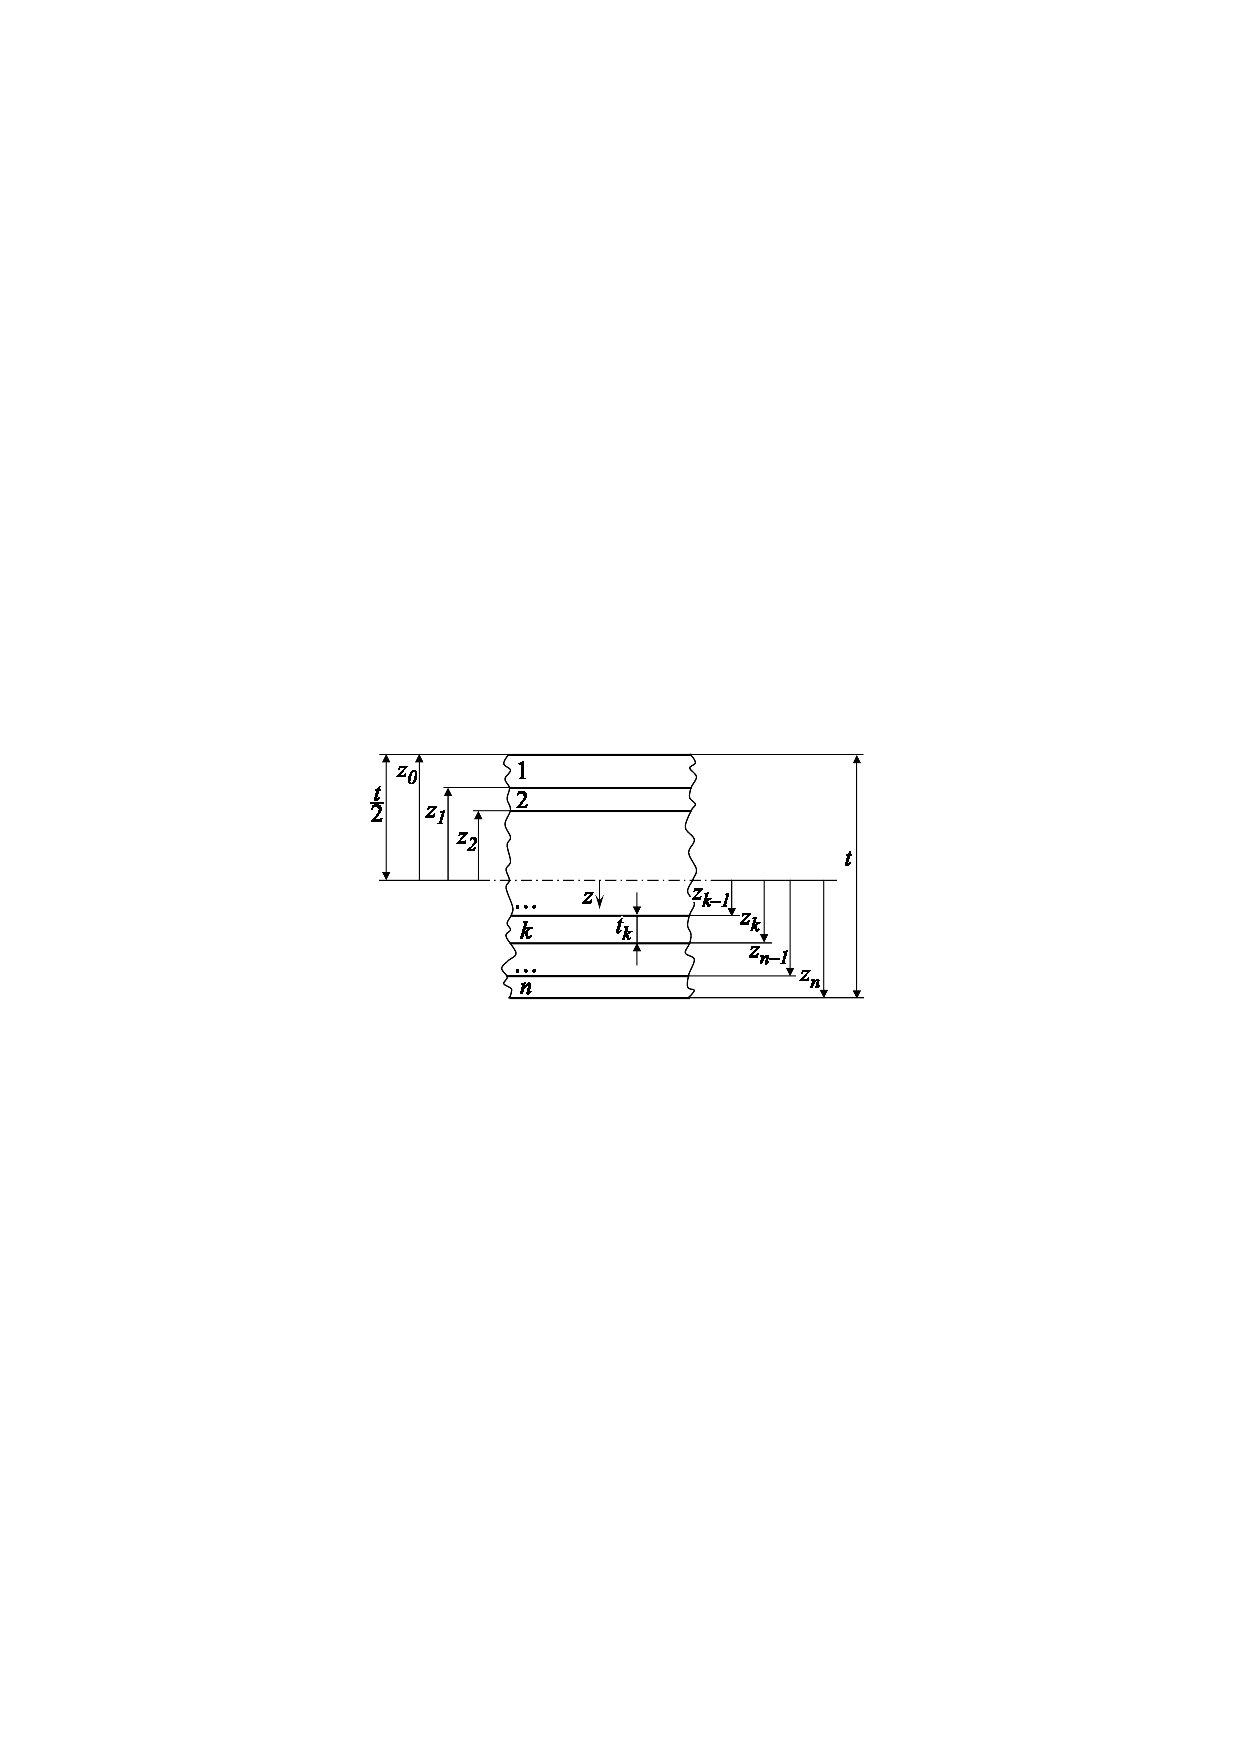
\includegraphics[width=85.0mm, height=42.0mm]{composite_layers}

    \caption{Иллюстрация модели многослойного композиционного материала (слоистого композита):}
    \label{fig:sloisty_kompozit}
    $t$ "--- толщина многослойной пластины; 1, 2, \dots, $k$, \dots, $n$ "--- номер слоя
\end{figure}

\begingroup
Напряжённое состояние многослойной пластины будет рассмотрено как плоское
напряжённое состояние \cites[14]{Alfutov1984_povorot_matric}, поскольку ранее
было принято допущение, что размеры пластины много больше её толщины.
Векторы и~матрицы в~уравнениях будут представлены в~сокращённой форме за~счёт
отбрасывания незадействованных компонентов
(сокращения до~размерности 3\(\,\times\,\)3).\russianpar
\endgroup

Поэтому уравнение~\eqref{eq:form_sigma_Q} может быть записано в~матричном
представлении следующим образом:
\[
\begin{pmatrix}
\sigma_{x}\\
\sigma_{y}\\
\tau_{xy}
\end{pmatrix}
=
\begin{pmatrix}
Q_{11} & Q_{12} & Q_{16}\\
Q_{12} & Q_{22} & Q_{26}\\
Q_{16} & Q_{26} & Q_{66}
\end{pmatrix}
\left(
    \begin{pmatrix}
    \epsilon_{x}^0\\
    \epsilon_{y}^0\\
    \gamma_{xy}^0
    \end{pmatrix}
+ z
    \begin{pmatrix}
    \kappa_{x}\\
    \kappa_{y}\\
    \kappa_{xy}
    \end{pmatrix}
-
    \begin{pmatrix}
    \epsilon_{x}^T\\
    \epsilon_{y}^T\\
    \gamma_{xy}^T
    \end{pmatrix}
\right)\!\!,
\]
где $\sigma_{x}$,  $\sigma_{y}$,  $\tau_{xy}$ "--- элементы вектора напряжений,~Па;
$Q_{ij}$ "--- элементы преобразованной матрицы жёсткости каждого слоя,~Па;
$\epsilon_{x}^0$, $\epsilon_{y}^0$, $\gamma_{xy}^0$ "--- элементы вектора относительного удлинения срединной поверхности многослойной композитной пластины;
$\kappa_{x}$, $\kappa_{y}$, $\kappa_{xy}$ "--- элементы векторного представления радиуса кривизны срединной поверхности многослойной композитной пластины,~1/м;
$\epsilon_{x}^T$, $\epsilon_{y}^T$, $\gamma_{xy}^T$~---~элементы вектора индуцированных деформаций, вызванных тепловой нагрузкой.

\begingroup%
Обобщённые силовые факторы, воздействующие на~пластину, определяются посредством интегрирования уравнения~\eqref{eq:form_sigma_Q} по~всей толщине пластины:\russianpar
\endgroup%
\[
\mathbf{N} = \int\limits_t \boldsymbol{\sigma} \mathrm{d}z,
\]
\[
\mathbf{M} = \int\limits_t \boldsymbol{\sigma} z \mathrm{d}z,
\]
где $t$ "--- толщина многослойной пластины, м;
$ \mathbf{N} $ "--- результирующая нагрузка, отнесённая к~единице длины линий, ограничивающих элемент рассматриваемой поверхности \cites[69]{Vasiljev1988_Meh_konstr_kompozit}, \mbox{Н/м};
$ \mathbf{M} $ "--- результирующий момент, отнесённый к~единице длины линий, ограничивающих элемент рассматриваемой поверхности, Н.

Жёсткость каждого слоя $\mathbf{Q}$~неизменна по~толщине слоя, поэтому можно записать:
\[
A_{ij} = \sum\limits_{k=1}^n (Q_{ij})_k (z_k - z_{k-1}),
\]
\[
B_{ij} = \frac{1}{2} \sum\limits_{k=1}^n (Q_{ij})_k (z_k^2 - z_{k-1}^2),
\]
\[
D_{ij} = \frac{1}{3} \sum\limits_{k=1}^n (Q_{ij})_k (z_k^3 - z_{k-1}^3),
\]
где $ A_{ij} $ "--- элементы матрицы жёсткости при растяжении (мембранной жёсткости) \cites[157]{kristensen1982_per_Vved_v_kompozit}[С.~70,~79]{Vasiljev1988_Meh_konstr_kompozit},~Н/м;
$ B_{ij} $ "--- элементы матрицы жёсткости изгиб\nb-растяжение (смешанной жёсткости), Н;
$ D_{ij} $ "--- элементы матрицы жёсткости при изгибе (изгибной жёсткости), Н$\cdot$м;
$ z_k $ "--- расстояние до~текущего слоя, измеряемое от~срединной поверхности (см.~Рисунок~\ref{fig:sloisty_kompozit}).

Тогда взаимосвязь нагрузок и~деформаций может быть представлена в~уравнениях в~матричной форме:
\begin{equation}\label{eq:n_m_eps_kap_simp_matrix_comb}
\left(
    \begin{array}{@{}c@{}}
        \mathbf{N} \\
        \mathbf{M}
    \end{array}
\right)
=
\left(
    \begin{array}{@{}cc@{}}
        \mathbf{A} & \mathbf{B} \\
        \mathbf{B} & \mathbf{D}
    \end{array}
\right)
\left(
    \begin{array}{@{}c@{}}
        \boldsymbol{\epsilon^0} \\
        \boldsymbol{\kappa}
    \end{array}
\right)
-
\left(
    \begin{array}{@{}c@{}}
        \mathbf{N}^T \\
        \mathbf{M}^T
    \end{array}
\right)\!\!,
\end{equation}
где вызванные тепловым воздействием:
$ \mathbf{N}^T $ "--- усилие, отнесённое к~единице длины линий,
ограничивающих элемент рассматриваемой поверхности, Н/м;
$ \mathbf{M}^T $ "--- момент силы, отнесённый к~единице длины линий,
ограничивающих элемент рассматриваемой поверхности, Н.

Преобразовав запись, получим:
\begin{equation}\label{eq:N_matrix}%
%\advance\thickmuskip -2mu%Only do this as a last resort http://tex.stackexchange.com/a/85091/79756
%\advance\medmuskip -1mu minus -1mu%Only do this as a last resort http://tex.stackexchange.com/a/85091/79756
\hspace{-1em}%
    \begin{pmatrix}
    N_{x}\\
    N_{y}\\
    N_{xy}
    \end{pmatrix}
    =
    \begin{pmatrix}
    A_{11} & A_{12} & A_{16}\\
    A_{12} & A_{22} & A_{26}\\
    A_{16} & A_{26} & A_{66}
    \end{pmatrix}
    \begin{pmatrix}
    \epsilon_{x}^0\\
    \epsilon_{y}^0\\
    \epsilon_{xy}^0
    \end{pmatrix}
    +
    \begin{pmatrix}
    B_{11} & B_{12} & B_{16}\\
    B_{12} & B_{22} & B_{26}\\
    B_{16} & B_{26} & B_{66}
    \end{pmatrix}
    \begin{pmatrix}
    \kappa_{x}\\
    \kappa_{y}\\
    \kappa_{xy}
    \end{pmatrix}
    -
    \begin{pmatrix}
    N_{x}^T\\
    N_{y}^T\\
    N_{xy}^T
    \end{pmatrix}\!\!,%
\end{equation}%
\begin{equation}\label{eq:M_matrix}%
%\advance\thickmuskip -3mu %Only do this as a last resort http://tex.stackexchange.com/a/85091/79756
%\advance\medmuskip -2mu minus -1mu%Only do this as a last resort http://tex.stackexchange.com/a/85091/79756
\hspace{-1em}%
    \begin{pmatrix}
    M_{x}\\
    M_{y}\\
    M_{xy}
    \end{pmatrix}
    =
    \begin{pmatrix}
    B_{11} & B_{12} & B_{16}\\
    B_{12} & B_{22} & B_{26}\\
    B_{16} & B_{26} & B_{66}
    \end{pmatrix}
    \begin{pmatrix}
    \epsilon_{x}^0\\
    \epsilon_{y}^0\\
    \epsilon_{xy}^0
    \end{pmatrix}
    +
    \begin{pmatrix}
    D_{11} & D_{12} & D_{16}\\
    D_{12} & D_{22} & D_{26}\\
    D_{16} & D_{26} & D_{66}
    \end{pmatrix}
    \begin{pmatrix}
    \kappa_{x}\\
    \kappa_{y}\\
    \kappa_{xy}
    \end{pmatrix}
    -
    \begin{pmatrix}
    M_{x}^T\\
    M_{y}^T\\
    M_{xy}^T
    \end{pmatrix}\!\!,
\end{equation}
где $ N_{ij} $ "--- элементы вектора результирующей нагрузки, отнесённой к~единице длины линий, ограничивающих элемент рассматриваемой поверхности, Н/м;
$ M_{ij} $ "--- элементы вектора результирующего момента, отнесённого к~единице длины линий, ограничивающих элемент рассматриваемой поверхности, Н;
$ N_{ij}^T $~---~элементы векторной записи усилия, вызванного тепловым воздействием, отнесённого к~единице длины линий, ограничивающих элемент рассматриваемой поверхности, \mbox{Н/м};
$ M_{ij}^T $ "--- элементы векторной записи момента силы, вызванного тепловым воздействием, отнесённого к~единице длины линий, ограничивающих элемент рассматриваемой поверхности, Н.

Силы и~моменты, вызванные тепловым воздействием, определяются следующими уравнениями:
\begin{equation}\label{eq:NT_integral}
\mathbf{N}^T = \int\limits_t \mathbf{Q} \boldsymbol{\epsilon}^T \mathrm{d}z,
\end{equation}
\begin{equation}\label{eq:MT_integral}
\mathbf{M}^T = \int\limits_t \mathbf{Q} \boldsymbol{\epsilon}^T z \mathrm{d}z.
\end{equation}

Уравнение~\eqref{eq:n_m_eps_kap_simp_matrix_comb} можно переписать следующим
образом, так как внешняя механическая нагрузка не приложена:
\[
\left(
    \begin{array}{c}
        \mathbf{N}^T \\
        \mathbf{M}^T
    \end{array}
\right)
=
\left(
    \begin{array}{cc}
        \mathbf{A} & \mathbf{B} \\
        \mathbf{B} & \mathbf{D}
    \end{array}
\right)
\left(
    \begin{array}{c}
        \boldsymbol{\epsilon^0} \\
        \boldsymbol{\kappa}
    \end{array}
\right)\!\!.
\]
Уравнения (\ref{eq:N_matrix},~\ref{eq:M_matrix}) можно переписать: %NEEDFIX Большой косяк, вызванный включением showonlyrefs из пакета mathtools проявившийся из-за использования \ref (нужно при showonlyrefs пользовать \refeq), но залитый в ВАК диссер изменять нельзя, так что это не подлежит исправлению в исходниках моей диссертации
\[
    \begin{pmatrix}
    N_{x}^T\\
    N_{y}^T\\
    N_{xy}^T
    \end{pmatrix}
    =
    \begin{pmatrix}
    A_{11} & A_{12} & A_{16}\\
    A_{12} & A_{22} & A_{26}\\
    A_{16} & A_{26} & A_{66}
    \end{pmatrix}
    \begin{pmatrix}
    \epsilon_{x}^0\\
    \epsilon_{y}^0\\
    \epsilon_{xy}^0
    \end{pmatrix}
    +
    \begin{pmatrix}
    B_{11} & B_{12} & B_{16}\\
    B_{12} & B_{22} & B_{26}\\
    B_{16} & B_{26} & B_{66}
    \end{pmatrix}
    \begin{pmatrix}
    \kappa_{x}\\
    \kappa_{y}\\
    \kappa_{xy}
    \end{pmatrix}\!\!,
\]
\[
    \begin{pmatrix}
    M_{x}^T\\
    M_{y}^T\\
    M_{xy}^T
    \end{pmatrix}
    =
    \begin{pmatrix}
    B_{11} & B_{12} & B_{16}\\
    B_{12} & B_{22} & B_{26}\\
    B_{16} & B_{26} & B_{66}
    \end{pmatrix}
    \begin{pmatrix}
    \epsilon_{x}^0\\
    \epsilon_{y}^0\\
    \epsilon_{xy}^0
    \end{pmatrix}
    +
    \begin{pmatrix}
    D_{11} & D_{12} & D_{16}\\
    D_{12} & D_{22} & D_{26}\\
    D_{16} & D_{26} & D_{66}
    \end{pmatrix}
    \begin{pmatrix}
    \kappa_{x}\\
    \kappa_{y}\\
    \kappa_{xy}
    \end{pmatrix}\!\!.
\]
Преобразуем эту систему уравнений:
\begin{multline}\label{eq:eps0_simpmatrix}
\boldsymbol{\epsilon^0} =
\left(
\mathbf{A^{\!\!-1}} %притягиваем показатель обратности матрицы
+
(\mathbf{A^{\!\!-1}B}) %притягиваем показатель обратности матрицы
(\mathbf{D} - \mathbf{B A^{\!\!-1}B})\mathbf{{}^{\!-1}} %\! притягиваем показатель обратности матрицы
(\mathbf{B A^{\!\!-1}})
\right)
\mathbf{N}^T
- \\ - %перенос формулы
(\mathbf{A^{\!\!-1}B}) %притягиваем показатель обратности матрицы
(\mathbf{D} - \mathbf{B A^{\!\!-1}B})\mathbf{{}^{\!-1}} %притягиваем показатель обратности матрицы
\mathbf{M}^T,
\end{multline}
\begin{equation}\label{eq:kappa_simpmatrix}
\boldsymbol{\kappa} =
-
(\mathbf{D} - \mathbf{B A^{\!\!-1}B})\mathbf{{}^{\!-1}}
(\mathbf{B A^{\!\!-1}})
\mathbf{N}^T
+
(\mathbf{D} - \mathbf{B A^{\!\!-1}B})\mathbf{{}^{\!-1}}
\mathbf{M}^T,
\end{equation}
где $ \mathbf{A} $ "--- матрица жёсткости при растяжении (мембранная жёсткость), Н/м;
$ \mathbf{B} $~---~матрица жёсткости изгиб\nb-растяжение (смешанная жёсткость), Н;
$ \mathbf{D} $~---~матрица жёсткости при изгибе (изгибная жёсткость), Н$\cdot$м.

Подстановкой уравнений (\ref{eq:NT_integral}---\ref{eq:kappa_simpmatrix}) %NEEDFIX Большой косяк, вызванный включением showonlyrefs из пакета mathtools проявившийся из-за использования \ref (нужно при showonlyrefs пользовать \refeq), но залитый в ВАК диссер изменять нельзя, так что это не подлежит исправлению в исходниках моей диссертации
в~уравнение~\eqref{eq:form_sigma_Q} получаем зависимость для определения
остаточных напряжений в~любой плоскости внутри рассматриваемой сборки
параллельной срединной поверхности:
\begin{multline*}
    \boldsymbol{\sigma}
    =
    \mathbf{Q}
    \left(
        \boldsymbol{\epsilon^0}
        +
        z
        \left(
            -
            (\mathbf{D} - \mathbf{B A^{\!\!-1}B})\mathbf{{}^{\!-1}} %притягиваем показатель обратности матрицы
            (\mathbf{B A^{\!\!-1}}) %притягиваем показатель обратности матрицы
            \mathbf{N}^T
            \right.\right. % фейк ради переноса
            + \\ +
            \left. % фейк ради переноса
            (\mathbf{D} - \mathbf{B A^{\!\!-1}B})\mathbf{{}^{\!-1}} %притягиваем показатель обратности матрицы
            \mathbf{M}^T
        \right)
        -
        \int\limits_{T_{b}}^{T_{w}}
        \left. % фейк ради переноса
        \boldsymbol{\alpha}(T)\:\mathrm{d}T
    \right).
\end{multline*}

Напряжения в~любых направлениях можно определять зная расположение главных осей
кремния, преобразуя значения элементов матриц жёсткости в~элементы матрицы
$\mathbf{Q}$~в~соответствии с~формулами поворота системы координат \cites[С.~18,~215,~224]{Alfutov1984_povorot_matric}.

Описанные модели, в частности модель двух тонких слоёв и модель
многослойного композиционного материала, позволяют, последовательно
увеличивая вычислительную сложность, оценивать остаточные напряжения
в~сплошных соединённых пластинах кремния и стекла. Уменьшение числа допущений
приводит к усложнению и дальнейшему развитию методов расчёта
напряжённо\nb-деформированного состояния многослойных
пластин~\cites[С.~165,~170]{kristensen1982_per_Vved_v_kompozit}{bitkina2013_avtoref}.
Однако, для наиболее точной оценки
остаточных напряжений в приборах с объёмной микрообработкой кремния
следует применять конечно-элементное
моделирование. Предварительное использование простых моделей, описанных
ранее в этой главе облегчает поиск оптимальных макроскопических параметров
моделей в~комплексах численного конечно-элементного моделирования.

\section{Результаты применения моделей}

\subsection{Исходные данные (характеристики применяемых материалов)}\label{chap_source_data}

Зависимости ТКЛР от температуры для стёкол марок Borofloat 33, ЛК5,
7740 и SD\nb-2 были получены автором экспериментально
термомеханическим анализатором TMA7100 с относительной погрешностью
${\pm}$5~\% (см.~подраздел~\ref{chap_cte_measure}). Данные
производителя по температурной зависимости ТКЛР стекла марки SW\nb-YY
приведены в~подразделе~\ref{GlassInfoOffic}. Для тех диапазонов
температур, которые выходили за границы, рассмотренные производителем,
использовались зависимости ТКЛР подобные имеющимся в известном
диапазоне температур. Упругие свойства вышеназванных стёкол также
приведены в~подразделе~\ref{GlassInfoOffic}.

На Рисунке~\ref{fig:cte}
приведены графики зависимостей ТКЛР от температуры для стёкол нескольких марок и кремния, использованные для расчётов в~этой главе.

\begin{figure}[!hb]%Порядок, в котором заданы опции, позволяющие регулировать положение рисунка на странице, не важен — они всегда будут применяться в порядке h (здесь) — t (вверху) — b (внизу) — p (на отдельной странице). Важно только то, какие именно опции заданы. По умолчанию — [tbp]. Задавать опции по одной (например, просто [t] или просто [b]) не рекомендуется — в некоторых случаях это может приводить к проблемным ситуациям.
    \centering
    \begingroup%
      \makeatletter%
      \providecommand\color[2][]{%
        \errmessage{(Inkscape) Color is used for the text in Inkscape, but the package 'color.sty' is not loaded}%
        \renewcommand\color[2][]{}%
      }%
      \providecommand\transparent[1]{%
        \errmessage{(Inkscape) Transparency is used (non-zero) for the text in Inkscape, but the package 'transparent.sty' is not loaded}%
        \renewcommand\transparent[1]{}%
      }%
      \providecommand\rotatebox[2]{#2}%
      \ifx\svgwidth\undefined%
        \setlength{\unitlength}{0.7\textwidth}%
        \ifx\svgscale\undefined%
          \relax%
        \else%
          \setlength{\unitlength}{\unitlength * \real{\svgscale}}%
        \fi%
      \else%
        \setlength{\unitlength}{\svgwidth}%
      \fi%
      \global\let\svgwidth\undefined%
      \global\let\svgscale\undefined%
      \makeatother%
      \begin{picture}(1,0.91078009)%
        \put(0,0){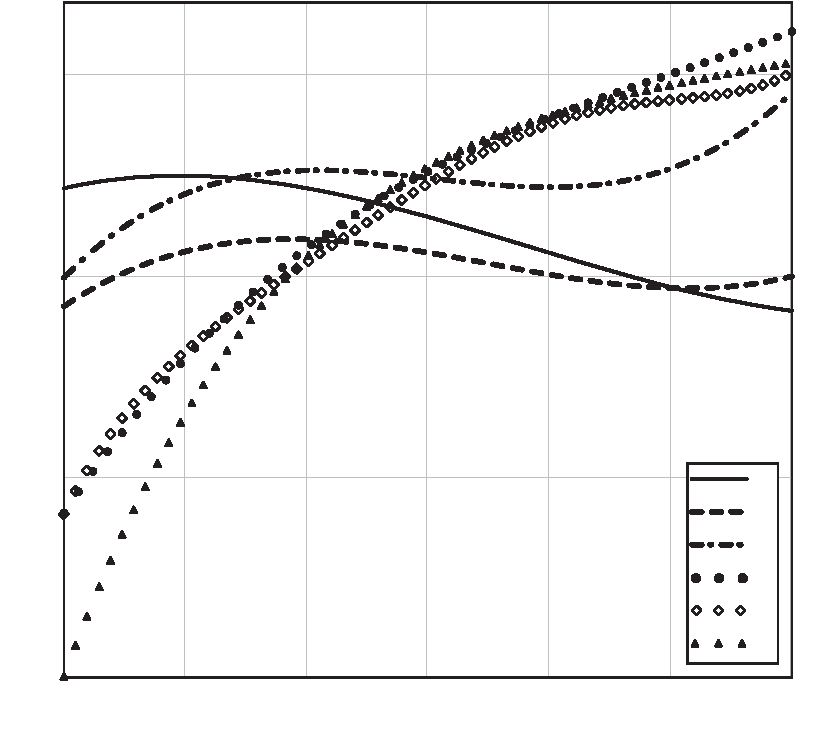
\includegraphics[width=\unitlength]{cte.pdf}}%
        \put(0.04942721,0.05233306){\color[named]{black}\makebox(0,0)[lb]{\smash{$-$100}}}%
        \put(0.22365626,0.05233304){\color[named]{black}\makebox(0,0)[lb]{\smash{0}}}%
        \put(0.35645273,0.05233304){\color[named]{black}\makebox(0,0)[lb]{\smash{100}}}%
        \put(0.50245295,0.05233304){\color[named]{black}\makebox(0,0)[lb]{\smash{200}}}%
        \put(0.65042616,0.05233304){\color[named]{black}\makebox(0,0)[lb]{\smash{300}}}%
        \put(0.79839936,0.05233304){\color[named]{black}\makebox(0,0)[lb]{\smash{400}}}%
        \put(0.0542787,0.3197472){\color[named]{black}\makebox(0,0)[lb]{\smash{2}}}%
        \put(0.05360435,0.56454799){\color[named]{black}\makebox(0,0)[lb]{\smash{3}}}%
        \put(0.0544862,0.80919695){\color[named]{black}\makebox(0,0)[lb]{\smash{4}}}%
        \put(0.92608635,0.32172017){\color[named]{black}\makebox(0,0)[b]{\smash{\textsl{1}}}}%
        \put(0.92608635,0.28180535){\color[named]{black}\makebox(0,0)[b]{\smash{\textsl{2}}}}%
        \put(0.92608635,0.24204229){\color[named]{black}\makebox(0,0)[b]{\smash{\textsl{3}}}}%
        \put(0.92608635,0.20212747){\color[named]{black}\makebox(0,0)[b]{\smash{\textsl{4}}}}%
        \put(0.92608635,0.16236441){\color[named]{black}\makebox(0,0)[b]{\smash{\textsl{5}}}}%
        \put(0.92608635,0.12244959){\color[named]{black}\makebox(0,0)[b]{\smash{\textsl{6}}}}%
        \put(0.02458804,0.38804245){\color[named]{black}\rotatebox{90}{\makebox(0,0)[lb]{\smash{$\alpha$, 10\textsuperscript{$-$6}~{\textdegree}C\textsuperscript{$-$1}}}}}%
        \put(0.94814375,0.05233306){\color[named]{black}\makebox(0,0)[lb]{\smash{500}}}%
        \put(0.05088963,0.0809656){\color[named]{black}\makebox(0,0)[lb]{\smash{1}}}%
        \put(0.48230067,0.00589629){\color[named]{black}\makebox(0,0)[lb]{\smash{$T$,~{\textdegree}C}}}%
      \end{picture}%
    \endgroup%

    \caption{Зависимости коэффициентов теплового линейного расширения от~температуры для нескольких марок стекла и кремния:}
    \label{fig:cte}
    \textsl{1} "--- Corning 7740,  \textsl{2} "--- Schott Borofloat 33,  \textsl{3} "--- ЛК5,  \textsl{4} "--- Hoya~SD-2,  \textsl{5}~---~Asahi~SW\nb-YY,  \textsl{6} "--- кремний%
\end{figure}

Упругие свойства пластины кремния ориентации \{100\} взяты из
\cites[42]{Bao_part_Mech_Beam_Diaphragm_Structures}.
Зависимость ТКЛР кремния от температуры приведена в~\cite{OkadaTokumaru_precise_silicon1984}. Для удобства использования в расчётах, она была переведена в полиномиальную форму:
\begin{multline}
    \alpha_{si}(T) = -3,268 \cdot 10^{-6} + 3,469 \cdot 10^{-8} \cdot T - 6,889 \cdot 10^{-11} \cdot T^2
    + \\  %перенос формулы
   + 6,991 \cdot 10^{-14} \cdot T^3 - 3,51 \cdot 10^{-17} \cdot T^4 + 6,916 \cdot 10^{-21} \cdot T^5,
\end{multline}

Во всех материалах с кубической кристаллической решёткой, в том числе и в кремнии, ТКЛР не зависит от направления измерения~\cite{slack1975thermal}.

\subsection{Методика определения температуры соединения из~анализа кривых зависимостей температурных коэффициентов линейного расширения}
Рассмотрим  простой способ определения оптимальной температуры соединения с
помощью модели двух тонких слоёв. Для примера возьмём случай, когда в одном
диапазоне температур коэффициент теплового расширения стекла больше коэффициента
теплового расширения кремния, а в другом диапазоне меньше. Таким образом, график
зависимости ТКЛР стекла от~температуры пересекает график зависимости ТКЛР
кремния. Иллюстрацией данной ситуации послужат графики для стекла ЛК5 и кремния
(см.~Рисунок~\ref{graphic_integ}).

\begin{figure}[!htb]%Порядок, в котором заданы опции, позволяющие регулировать положение рисунка на странице, не важен — они всегда будут применяться в порядке h (здесь) — t (вверху) — b (внизу) — p (на отдельной странице). Важно только то, какие именно опции заданы. По умолчанию — [tbp]. Задавать опции по одной (например, просто [t] или просто [b]) не рекомендуется — в некоторых случаях это может приводить к проблемным ситуациям.
    \centering
    \noindent%
    \begingroup%
      \makeatletter%
      \ifx\svgwidth\undefined%
        \setlength{\unitlength}{0.54\textwidth}%
        \ifx\svgscale\undefined%
          \relax%
        \else%
          \setlength{\unitlength}{\unitlength * \real{\svgscale}}%
        \fi%
      \else%
        \setlength{\unitlength}{\svgwidth}%
      \fi%
      \global\let\svgwidth\undefined%
      \global\let\svgscale\undefined%
      \makeatother%
      \begin{picture}(1,0.75870968)%
        \put(0,0){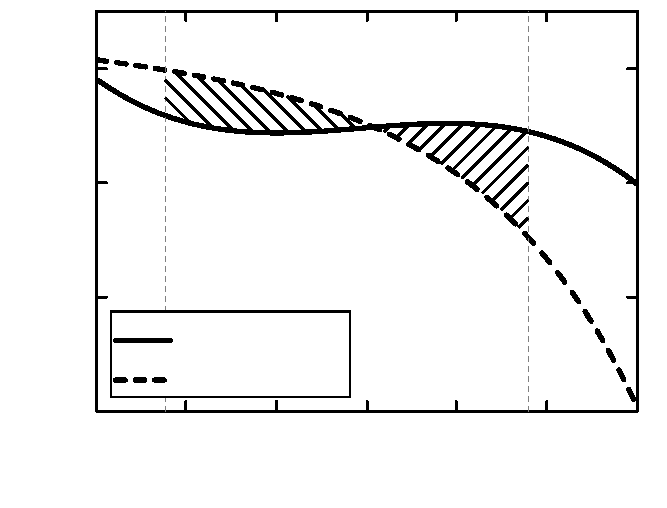
\includegraphics[width=\unitlength]{graphic_integ_lk5_mirror}}%
        \put(0.13379818,0.13843943){\color[named]{black}\makebox(0,0)[rb]{\smash{1}}}%
        \put(0.13198206,0.30434553){\color[named]{black}\makebox(0,0)[rb]{\smash{2}}}%
        \put(0.13243075,0.47250155){\color[named]{black}\makebox(0,0)[rb]{\smash{3}}}%
        \put(0.13125561,0.64322094){\color[named]{black}\makebox(0,0)[rb]{\smash{4}}}%
        \put(0.14691889,0.08513952){\color[named]{black}\makebox(0,0)[b]{\smash{500}}}%
        \put(0.28063032,0.08513952){\color[named]{black}\makebox(0,0)[b]{\smash{400}}}%
        \put(0.41659216,0.08513952){\color[named]{black}\makebox(0,0)[b]{\smash{300}}}%
        \put(0.552554,0.08513952){\color[named]{black}\makebox(0,0)[b]{\smash{200}}}%
        \put(0.68607791,0.08513952){\color[named]{black}\makebox(0,0)[b]{\smash{100}}}%
        \put(0.82078945,0.08513952){\color[named]{black}\makebox(0,0)[b]{\smash{0}}}%
        \put(0.94206112,0.08513952){\color[named]{black}\makebox(0,0)[b]{\smash{$-$100}}}%
        \put(0.06309799,0.44107293){\color[named]{black}\rotatebox{90}{\makebox(0,0)[b]{\smash{ТКЛР, 10\textsuperscript{$-$6}{\textdegree}C\textsuperscript{$-$1}}}}}%
        \put(0.26708896,0.23391665){\color[named]{black}\makebox(0,0)[lb]{\smash{ЛК5}}}%
        \put(0.26447009,0.17756749){\color[named]{black}\makebox(0,0)[lb]{\smash{Кремний}}}%
        \put(0.79069249,0.685){\color[named]{black}\makebox(0,0)[b]{\smash{20}}}%
        \put(0.24981493,0.685){\color[named]{black}\makebox(0,0)[b]{\smash{422}}}%
      \end{picture}%
    \endgroup%

    \noindent%
    \begingroup%
      \makeatletter%
      \ifx\svgwidth\undefined%
        \setlength{\unitlength}{0.54\textwidth}%
        \ifx\svgscale\undefined%
          \relax%
        \else%
          \setlength{\unitlength}{\unitlength * \real{\svgscale}}%
        \fi%
      \else%
        \setlength{\unitlength}{\svgwidth}%
      \fi%
      \global\let\svgwidth\undefined%
      \global\let\svgscale\undefined%
      \makeatother%
      \begin{picture}(1,0.77746311)%
        \put(0,0){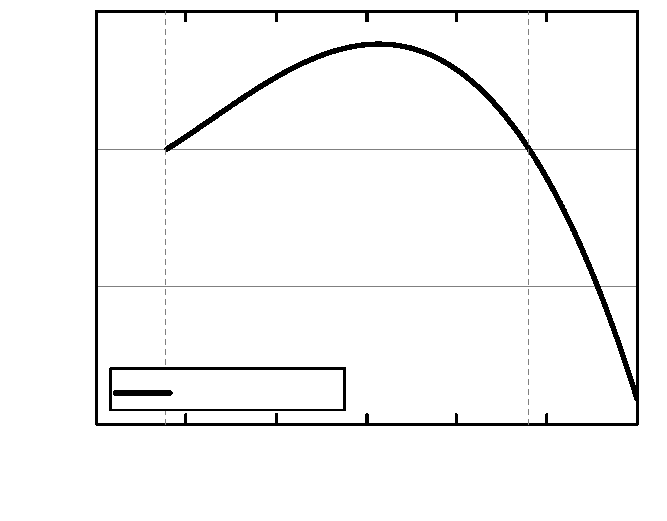
\includegraphics[width=\unitlength]{graphic_integ_lk5_sigma}}%
        \put(0.1330892,0.12928924){\color[named]{black}\makebox(0,0)[rb]{\smash{$-$10}}}%
        \put(0.13274734,0.33651364){\color[named]{black}\makebox(0,0)[rb]{\smash{$-$5}}}%
        \put(0.1330892,0.54117533){\color[named]{black}\makebox(0,0)[rb]{\smash{0}}}%
        \put(0.13274734,0.74564893){\color[named]{black}\makebox(0,0)[rb]{\smash{5}}}%
        \put(0.03769707,0.46873699){\color[named]{black}\rotatebox{90}{\makebox(0,0)[b]{\smash{Напряжения, МПа}}}}%
        \put(0.55242838,0.01292082){\color[named]{black}\makebox(0,0)[b]{\smash{Температура,{\textdegree}C}}}%
        \put(0.14705445,0.08375692){\color[named]{black}\makebox(0,0)[b]{\smash{500}}}%
        \put(0.28076591,0.08375692){\color[named]{black}\makebox(0,0)[b]{\smash{400}}}%
        \put(0.41672777,0.08375692){\color[named]{black}\makebox(0,0)[b]{\smash{300}}}%
        \put(0.55268964,0.08375692){\color[named]{black}\makebox(0,0)[b]{\smash{200}}}%
        \put(0.68621509,0.08375692){\color[named]{black}\makebox(0,0)[b]{\smash{100}}}%
        \put(0.82092923,0.08375692){\color[named]{black}\makebox(0,0)[b]{\smash{0}}}%
        \put(0.94720432,0.08375692){\color[named]{black}\makebox(0,0)[b]{\smash{$-$100}}}%
        \put(0.2457595,0.69886941){\color[named]{black}\makebox(0,0)[b]{\smash{422}}}%
        \put(0.79085926,0.69886941){\color[named]{black}\makebox(0,0)[b]{\smash{20}}}%
        \put(0.26933091,0.17707933){\color[named]{black}\makebox(0,0)[lb]{\smash{Кремний}}}%
      \end{picture}%
    \endgroup%

    \caption{Иллюстрация графического интегрирования на примере соединения стекла ЛК5 с кремнием}
    \label{graphic_integ}
\end{figure}

При температуре соединения, в данном примере 422~{\textdegree}C,
в соединённых пластинах не возникает остаточных напряжений.
Несоединённые кремний и~стекло имеют одинаковую длину.

В процессе дальнейшего охлаждения, пока $\alpha_{si} > \alpha_{g}$
(кремний сжимается быстрее стекла до температуры примерно 190~{\textdegree}C в случае стекла ЛК5, см.~Рисунок~\ref{graphic_integ}), увеличивается прогиб пластин (вогнутостью
в сторону пластины кремния). Также увеличиваются растягивающие напряжения внутри
пластины кремния.

Когда при дальнейшем охлаждении приходим к точке совпадения значений истинных
коэффциентов теплового расширения кремния и стекла $\alpha_{si} = \alpha_{g}$ %NEEDFIX здесь опечатка в слове «коэффИциентов», но залитый в ВАК диссер изменять нельзя, так что это не подлежит исправлению в исходниках моей диссертации
(примерно около температуры 190~{\textdegree}C для стекла ЛК5), прогиб перестаёт увеличиваться,
достигнув максимального значения. Перестают увеличиваться и~растягивающие
напряжения в кремнии.
Несоединённый кремний был бы всё ещё короче стекла.

При продолжении охлаждения кремний сжимается медленнее стекла
\mbox{($\alpha_{si} < \alpha_{g}$)}. Величина прогиба начинает уменьшаться.
Растягивающие напряжения в кремнии так же пропорционально снижаются.

При достижении комнатной температуры (для данного примера, см.
Рисунок~\ref{graphic_integ}), совокупная накопленная деформация становится
нулевой. Отсутствует прогиб пластин и остаточные напряжения в кремнии и стекле
равны нулю.
Если бы кремний и стекло не были соединены, они снова были бы~одинаковой длины.

Если продолжить охлаждать, то за счёт того, что кремний сжимается медленнее
стекла ($\alpha_{si} < \alpha_{g}$), пластины продолжат изгибаться. Теперь
вогнутость будет в сторону пластины стекла. При этом в кремнии будут формироваться
остаточные сжимающие напряжения.

Определить температуру проведения процесса электростатического соединения,
обеспечивающую отсутствие напряжений при заданной рабочей температуре, можно
графически. Области, отсечённые линиями температур и графиков ТКЛР стекла и
кремния по обе стороны от точки пересечения графиков ТКЛР, должны быть равными
(см. Рисунок~\ref{graphic_integ}). Это утверждение также вытекает
из~формулы~\eqref{eq:sigma_siupdated}. Для ЛК5 и рабочей температуры
20~{\textdegree}C температура соединения, обеспечивающая отсутствие остаточных
напряжений, составляет 422~{\textdegree}C.

Для рассматриваемых марок боросиликатных стёкол (ЛК5, 7740, Borofloat~33) точка
пересечения кривых температурных зависимостей ТКЛР располагается при
температурах ниже типичных температур проведения анодной посадки. Таким образом,
для определения температуры ненапряжённого соединения можно заключить, что
интеграл разности температурных зависимостей ТКЛР стекла и кремния от рабочей
температуры до температуры в~момент подачи высокого напряжения должен равняться
нулю.

Расчётные значения накапливаемой относительной деформации приведены на
Рисунке~\ref{fig:nakop_deform}.
Графики построены на основе следующей формулы:
\begin{equation}
    \label{eq:nakop_deform}
    \frac {\Delta l}{l_0}
    =
    \int\limits_{T_b}^{T_w}
    (
         \alpha_g(T) - \alpha_{si}(T)
    )
    \:\mathrm{d}T.
\end{equation}

Из Рисунка~\ref{fig:nakop_deform} видно, что каждое стекло влияет по-разному
на напряжения в кремнии в рабочем диапазоне температур. Увеличение температуры
сращивания кремния со стеклом \(T_b\) увеличивает растягивающие напряжения
в~стекле для четырёх из пяти рассматриваемых марок стёкол (исключая Hoya SD-2).
Из-за различий в ТКЛР (главным образом из-за разной температуры пересечения
с ТКЛР кремния, см. Рисунок~\ref{fig:cte}) остаточные напряжения, вызываемые
стеклом ЛК5, более сжимающие и, в то же время, меньше зависят от выбора
температуры сращивания, чем напряжения, вызываемые стёклами Borofloat~33 и
Corning 7740. Изменение температуры сращивания с алюмосиликатными стёклами (SD-2
и SW-YY) оказывает заметно меньшее влияние на остаточные напряжения, чем с
боросиликатными стёклами (Borofloat~33, Corning 7740 и ЛК5). Также
Рисунок~\ref{fig:nakop_deform} иллюстрирует, что идея «снижение температуры
сращивания снижает остаточные напряжения» верна лишь для определённых марок
стекла или даже для определённых партий стекла, поскольку зависимость ТКЛР от
температуры может отличаться от~партии к~партии. Например, снижение температуры
соединения кремния со стеклом ЛК5 лишь повышает сжимающие напряжения в кремнии
(согласно модели двух тонких слоёв). Видно, что утверждение о наличии
температуры ненапряжённого сращивания~\cite{Cozma_Puers_1995} верно лишь для
конкретной заданной рабочей температуры \(T_w\). В~диапазоне температур
остаточные напряжения будут изменяться.

\begin{figure}[!htb]%Порядок, в котором заданы опции, позволяющие регулировать положение рисунка на странице, не важен — они всегда будут применяться в порядке h (здесь) — t (вверху) — b (внизу) — p (на отдельной странице). Важно только то, какие именно опции заданы. По умолчанию — [tbp]. Задавать опции по одной (например, просто [t] или просто [b]) не рекомендуется — в некоторых случаях это может приводить к проблемным ситуациям.
    \centering
    \ifdefmacro{\tikzsetnextfilename}{\tikzsetnextfilename{nakop_deform}}{}%
    \begin{tikzpicture}[x=1pt,y=1pt]
\definecolor{fillColor}{RGB}{255,255,255}
\path[use as bounding box,fill=fillColor] (0,0) rectangle (497.92,398.34);
\begin{scope}
\path[clip] (  0.00,  0.00) rectangle (497.92,398.34);
\definecolor{drawColor}{RGB}{255,255,255}

\path[draw=drawColor,line width= 0.6pt,line join=round,line cap=round,fill=fillColor] (  0.00,  0.00) rectangle (497.92,398.34);
\end{scope}
\begin{scope}
\path[clip] ( 38.21,217.69) rectangle (186.04,376.42);
\definecolor{fillColor}{RGB}{255,255,255}

\path[fill=fillColor] ( 38.21,217.69) rectangle (186.04,376.42);
\definecolor{drawColor}{gray}{0.98}

\path[draw=drawColor,line width= 0.6pt,line join=round] ( 38.21,224.93) --
	(186.04,224.93);

\path[draw=drawColor,line width= 0.6pt,line join=round] ( 38.21,263.86) --
	(186.04,263.86);

\path[draw=drawColor,line width= 0.6pt,line join=round] ( 38.21,302.79) --
	(186.04,302.79);

\path[draw=drawColor,line width= 0.6pt,line join=round] ( 38.21,341.72) --
	(186.04,341.72);

\path[draw=drawColor,line width= 0.6pt,line join=round] ( 72.74,217.69) --
	( 72.74,376.42);

\path[draw=drawColor,line width= 0.6pt,line join=round] (109.81,217.69) --
	(109.81,376.42);

\path[draw=drawColor,line width= 0.6pt,line join=round] (137.62,217.69) --
	(137.62,376.42);

\path[draw=drawColor,line width= 0.6pt,line join=round] (167.74,217.69) --
	(167.74,376.42);
\definecolor{drawColor}{gray}{0.90}

\path[draw=drawColor,line width= 0.2pt,line join=round] ( 38.21,244.39) --
	(186.04,244.39);

\path[draw=drawColor,line width= 0.2pt,line join=round] ( 38.21,283.32) --
	(186.04,283.32);

\path[draw=drawColor,line width= 0.2pt,line join=round] ( 38.21,322.25) --
	(186.04,322.25);

\path[draw=drawColor,line width= 0.2pt,line join=round] ( 38.21,361.19) --
	(186.04,361.19);

\path[draw=drawColor,line width= 0.2pt,line join=round] ( 44.93,217.69) --
	( 44.93,376.42);

\path[draw=drawColor,line width= 0.2pt,line join=round] (100.54,217.69) --
	(100.54,376.42);

\path[draw=drawColor,line width= 0.2pt,line join=round] (119.08,217.69) --
	(119.08,376.42);

\path[draw=drawColor,line width= 0.2pt,line join=round] (156.15,217.69) --
	(156.15,376.42);

\path[draw=drawColor,line width= 0.2pt,line join=round] (179.32,217.69) --
	(179.32,376.42);
\definecolor{drawColor}{RGB}{0,0,0}

\path[draw=drawColor,line width= 1.4pt,line join=round] ( 44.93,236.47) --
	( 45.39,236.84) --
	( 45.86,237.20) --
	( 46.32,237.56) --
	( 46.78,237.92) --
	( 47.25,238.28) --
	( 47.71,238.63) --
	( 48.18,238.99) --
	( 48.64,239.34) --
	( 49.10,239.70) --
	( 49.57,240.05) --
	( 50.03,240.40) --
	( 50.49,240.75) --
	( 50.96,241.10) --
	( 51.42,241.44) --
	( 51.88,241.79) --
	( 52.35,242.13) --
	( 52.81,242.48) --
	( 53.27,242.82) --
	( 53.74,243.16) --
	( 54.20,243.50) --
	( 54.66,243.84) --
	( 55.13,244.17) --
	( 55.59,244.51) --
	( 56.05,244.84) --
	( 56.52,245.18) --
	( 56.98,245.51) --
	( 57.44,245.84) --
	( 57.91,246.17) --
	( 58.37,246.50) --
	( 58.83,246.83) --
	( 59.30,247.16) --
	( 59.76,247.48) --
	( 60.22,247.81) --
	( 60.69,248.13) --
	( 61.15,248.45) --
	( 61.61,248.77) --
	( 62.08,249.09) --
	( 62.54,249.41) --
	( 63.00,249.73) --
	( 63.47,250.04) --
	( 63.93,250.36) --
	( 64.40,250.67) --
	( 64.86,250.98) --
	( 65.32,251.30) --
	( 65.79,251.61) --
	( 66.25,251.92) --
	( 66.71,252.22) --
	( 67.18,252.53) --
	( 67.64,252.84) --
	( 68.10,253.14) --
	( 68.57,253.44) --
	( 69.03,253.75) --
	( 69.49,254.05) --
	( 69.96,254.35) --
	( 70.42,254.65) --
	( 70.88,254.95) --
	( 71.35,255.24) --
	( 71.81,255.54) --
	( 72.27,255.83) --
	( 72.74,256.13) --
	( 73.20,256.42) --
	( 73.66,256.71) --
	( 74.13,257.00) --
	( 74.59,257.29) --
	( 75.05,257.58) --
	( 75.52,257.86) --
	( 75.98,258.15) --
	( 76.44,258.44) --
	( 76.91,258.72) --
	( 77.37,259.00) --
	( 77.83,259.28) --
	( 78.30,259.56) --
	( 78.76,259.84) --
	( 79.22,260.12) --
	( 79.69,260.40) --
	( 80.15,260.67) --
	( 80.61,260.95) --
	( 81.08,261.22) --
	( 81.54,261.50) --
	( 82.01,261.77) --
	( 82.47,262.04) --
	( 82.93,262.31) --
	( 83.40,262.58) --
	( 83.86,262.84) --
	( 84.32,263.11) --
	( 84.79,263.38) --
	( 85.25,263.64) --
	( 85.71,263.90) --
	( 86.18,264.17) --
	( 86.64,264.43) --
	( 87.10,264.69) --
	( 87.57,264.95) --
	( 88.03,265.21) --
	( 88.49,265.46) --
	( 88.96,265.72) --
	( 89.42,265.97) --
	( 89.88,266.23) --
	( 90.35,266.48) --
	( 90.81,266.73) --
	( 91.27,266.98) --
	( 91.74,267.23) --
	( 92.20,267.48) --
	( 92.66,267.73) --
	( 93.13,267.98) --
	( 93.59,268.22) --
	( 94.05,268.47) --
	( 94.52,268.71) --
	( 94.98,268.96) --
	( 95.44,269.20) --
	( 95.91,269.44) --
	( 96.37,269.68) --
	( 96.83,269.92) --
	( 97.30,270.15) --
	( 97.76,270.39) --
	( 98.22,270.63) --
	( 98.69,270.86) --
	( 99.15,271.10) --
	( 99.62,271.33) --
	(100.08,271.56) --
	(100.54,271.79) --
	(101.01,272.02) --
	(101.47,272.25) --
	(101.93,272.48) --
	(102.40,272.70) --
	(102.86,272.93) --
	(103.32,273.16) --
	(103.79,273.38) --
	(104.25,273.60) --
	(104.71,273.83) --
	(105.18,274.05) --
	(105.64,274.27) --
	(106.10,274.49) --
	(106.57,274.70) --
	(107.03,274.92) --
	(107.49,275.14) --
	(107.96,275.35) --
	(108.42,275.57) --
	(108.88,275.78) --
	(109.35,275.99) --
	(109.81,276.20) --
	(110.27,276.42) --
	(110.74,276.63) --
	(111.20,276.83) --
	(111.66,277.04) --
	(112.13,277.25) --
	(112.59,277.45) --
	(113.05,277.66) --
	(113.52,277.86) --
	(113.98,278.07) --
	(114.44,278.27) --
	(114.91,278.47) --
	(115.37,278.67) --
	(115.84,278.87) --
	(116.30,279.07) --
	(116.76,279.27) --
	(117.23,279.46) --
	(117.69,279.66) --
	(118.15,279.85) --
	(118.62,280.05) --
	(119.08,280.24) --
	(119.54,280.43) --
	(120.01,280.62) --
	(120.47,280.81) --
	(120.93,281.00) --
	(121.40,281.19) --
	(121.86,281.38) --
	(122.32,281.57) --
	(122.79,281.75) --
	(123.25,281.94) --
	(123.71,282.12) --
	(124.18,282.30) --
	(124.64,282.49) --
	(125.10,282.67) --
	(125.57,282.85) --
	(126.03,283.03) --
	(126.49,283.21) --
	(126.96,283.38) --
	(127.42,283.56) --
	(127.88,283.74) --
	(128.35,283.91) --
	(128.81,284.09) --
	(129.27,284.26) --
	(129.74,284.43) --
	(130.20,284.60) --
	(130.66,284.77) --
	(131.13,284.94) --
	(131.59,285.11) --
	(132.05,285.28) --
	(132.52,285.45) --
	(132.98,285.61) --
	(133.45,285.78) --
	(133.91,285.95) --
	(134.37,286.11) --
	(134.84,286.27) --
	(135.30,286.43) --
	(135.76,286.60) --
	(136.23,286.76) --
	(136.69,286.92) --
	(137.15,287.07) --
	(137.62,287.23) --
	(138.08,287.39) --
	(138.54,287.55) --
	(139.01,287.70) --
	(139.47,287.86) --
	(139.93,288.01) --
	(140.40,288.16) --
	(140.86,288.31) --
	(141.32,288.47) --
	(141.79,288.62) --
	(142.25,288.77) --
	(142.71,288.91) --
	(143.18,289.06) --
	(143.64,289.21) --
	(144.10,289.36) --
	(144.57,289.50) --
	(145.03,289.65) --
	(145.49,289.79) --
	(145.96,289.93) --
	(146.42,290.07) --
	(146.88,290.22) --
	(147.35,290.36) --
	(147.81,290.50) --
	(148.27,290.63) --
	(148.74,290.77) --
	(149.20,290.91) --
	(149.66,291.05) --
	(150.13,291.18) --
	(150.59,291.32) --
	(151.06,291.45) --
	(151.52,291.58) --
	(151.98,291.72) --
	(152.45,291.85) --
	(152.91,291.98) --
	(153.37,292.11) --
	(153.84,292.24) --
	(154.30,292.37) --
	(154.76,292.50) --
	(155.23,292.62) --
	(155.69,292.75) --
	(156.15,292.87) --
	(156.62,293.00) --
	(157.08,293.12) --
	(157.54,293.25) --
	(158.01,293.37) --
	(158.47,293.49) --
	(158.93,293.61) --
	(159.40,293.73) --
	(159.86,293.85) --
	(160.32,293.97) --
	(160.79,294.09) --
	(161.25,294.20) --
	(161.71,294.32) --
	(162.18,294.43) --
	(162.64,294.55) --
	(163.10,294.66) --
	(163.57,294.77) --
	(164.03,294.89) --
	(164.49,295.00) --
	(164.96,295.11) --
	(165.42,295.22) --
	(165.88,295.33) --
	(166.35,295.44) --
	(166.81,295.54) --
	(167.27,295.65) --
	(167.74,295.76) --
	(168.20,295.86) --
	(168.67,295.97) --
	(169.13,296.07) --
	(169.59,296.18) --
	(170.06,296.28) --
	(170.52,296.38) --
	(170.98,296.48) --
	(171.45,296.58) --
	(171.91,296.68) --
	(172.37,296.78) --
	(172.84,296.88) --
	(173.30,296.98) --
	(173.76,297.07) --
	(174.23,297.17) --
	(174.69,297.26) --
	(175.15,297.36) --
	(175.62,297.45) --
	(176.08,297.54) --
	(176.54,297.64) --
	(177.01,297.73) --
	(177.47,297.82) --
	(177.93,297.91) --
	(178.40,298.00) --
	(178.86,298.09) --
	(179.32,298.18);

\path[draw=drawColor,line width= 1.4pt,dash pattern=on 7pt off 3pt ,line join=round] ( 44.93,260.10) --
	( 45.39,260.46) --
	( 45.86,260.83) --
	( 46.32,261.19) --
	( 46.78,261.55) --
	( 47.25,261.90) --
	( 47.71,262.26) --
	( 48.18,262.62) --
	( 48.64,262.97) --
	( 49.10,263.32) --
	( 49.57,263.67) --
	( 50.03,264.03) --
	( 50.49,264.37) --
	( 50.96,264.72) --
	( 51.42,265.07) --
	( 51.88,265.42) --
	( 52.35,265.76) --
	( 52.81,266.10) --
	( 53.27,266.44) --
	( 53.74,266.79) --
	( 54.20,267.13) --
	( 54.66,267.46) --
	( 55.13,267.80) --
	( 55.59,268.14) --
	( 56.05,268.47) --
	( 56.52,268.81) --
	( 56.98,269.14) --
	( 57.44,269.47) --
	( 57.91,269.80) --
	( 58.37,270.13) --
	( 58.83,270.46) --
	( 59.30,270.78) --
	( 59.76,271.11) --
	( 60.22,271.43) --
	( 60.69,271.76) --
	( 61.15,272.08) --
	( 61.61,272.40) --
	( 62.08,272.72) --
	( 62.54,273.04) --
	( 63.00,273.35) --
	( 63.47,273.67) --
	( 63.93,273.98) --
	( 64.40,274.30) --
	( 64.86,274.61) --
	( 65.32,274.92) --
	( 65.79,275.23) --
	( 66.25,275.54) --
	( 66.71,275.85) --
	( 67.18,276.16) --
	( 67.64,276.46) --
	( 68.10,276.77) --
	( 68.57,277.07) --
	( 69.03,277.37) --
	( 69.49,277.68) --
	( 69.96,277.98) --
	( 70.42,278.28) --
	( 70.88,278.57) --
	( 71.35,278.87) --
	( 71.81,279.17) --
	( 72.27,279.46) --
	( 72.74,279.75) --
	( 73.20,280.05) --
	( 73.66,280.34) --
	( 74.13,280.63) --
	( 74.59,280.92) --
	( 75.05,281.21) --
	( 75.52,281.49) --
	( 75.98,281.78) --
	( 76.44,282.06) --
	( 76.91,282.35) --
	( 77.37,282.63) --
	( 77.83,282.91) --
	( 78.30,283.19) --
	( 78.76,283.47) --
	( 79.22,283.75) --
	( 79.69,284.03) --
	( 80.15,284.30) --
	( 80.61,284.58) --
	( 81.08,284.85) --
	( 81.54,285.12) --
	( 82.01,285.40) --
	( 82.47,285.67) --
	( 82.93,285.94) --
	( 83.40,286.20) --
	( 83.86,286.47) --
	( 84.32,286.74) --
	( 84.79,287.00) --
	( 85.25,287.27) --
	( 85.71,287.53) --
	( 86.18,287.79) --
	( 86.64,288.06) --
	( 87.10,288.32) --
	( 87.57,288.58) --
	( 88.03,288.83) --
	( 88.49,289.09) --
	( 88.96,289.35) --
	( 89.42,289.60) --
	( 89.88,289.86) --
	( 90.35,290.11) --
	( 90.81,290.36) --
	( 91.27,290.61) --
	( 91.74,290.86) --
	( 92.20,291.11) --
	( 92.66,291.36) --
	( 93.13,291.61) --
	( 93.59,291.85) --
	( 94.05,292.10) --
	( 94.52,292.34) --
	( 94.98,292.58) --
	( 95.44,292.82) --
	( 95.91,293.07) --
	( 96.37,293.31) --
	( 96.83,293.54) --
	( 97.30,293.78) --
	( 97.76,294.02) --
	( 98.22,294.25) --
	( 98.69,294.49) --
	( 99.15,294.72) --
	( 99.62,294.96) --
	(100.08,295.19) --
	(100.54,295.42) --
	(101.01,295.65) --
	(101.47,295.88) --
	(101.93,296.11) --
	(102.40,296.33) --
	(102.86,296.56) --
	(103.32,296.78) --
	(103.79,297.01) --
	(104.25,297.23) --
	(104.71,297.45) --
	(105.18,297.67) --
	(105.64,297.89) --
	(106.10,298.11) --
	(106.57,298.33) --
	(107.03,298.55) --
	(107.49,298.76) --
	(107.96,298.98) --
	(108.42,299.19) --
	(108.88,299.41) --
	(109.35,299.62) --
	(109.81,299.83) --
	(110.27,300.04) --
	(110.74,300.25) --
	(111.20,300.46) --
	(111.66,300.67) --
	(112.13,300.88) --
	(112.59,301.08) --
	(113.05,301.29) --
	(113.52,301.49) --
	(113.98,301.69) --
	(114.44,301.90) --
	(114.91,302.10) --
	(115.37,302.30) --
	(115.84,302.50) --
	(116.30,302.70) --
	(116.76,302.89) --
	(117.23,303.09) --
	(117.69,303.29) --
	(118.15,303.48) --
	(118.62,303.67) --
	(119.08,303.87) --
	(119.54,304.06) --
	(120.01,304.25) --
	(120.47,304.44) --
	(120.93,304.63) --
	(121.40,304.82) --
	(121.86,305.01) --
	(122.32,305.19) --
	(122.79,305.38) --
	(123.25,305.56) --
	(123.71,305.75) --
	(124.18,305.93) --
	(124.64,306.11) --
	(125.10,306.29) --
	(125.57,306.47) --
	(126.03,306.65) --
	(126.49,306.83) --
	(126.96,307.01) --
	(127.42,307.19) --
	(127.88,307.36) --
	(128.35,307.54) --
	(128.81,307.71) --
	(129.27,307.89) --
	(129.74,308.06) --
	(130.20,308.23) --
	(130.66,308.40) --
	(131.13,308.57) --
	(131.59,308.74) --
	(132.05,308.91) --
	(132.52,309.08) --
	(132.98,309.24) --
	(133.45,309.41) --
	(133.91,309.57) --
	(134.37,309.74) --
	(134.84,309.90) --
	(135.30,310.06) --
	(135.76,310.22) --
	(136.23,310.38) --
	(136.69,310.54) --
	(137.15,310.70) --
	(137.62,310.86) --
	(138.08,311.02) --
	(138.54,311.17) --
	(139.01,311.33) --
	(139.47,311.48) --
	(139.93,311.64) --
	(140.40,311.79) --
	(140.86,311.94) --
	(141.32,312.09) --
	(141.79,312.24) --
	(142.25,312.39) --
	(142.71,312.54) --
	(143.18,312.69) --
	(143.64,312.84) --
	(144.10,312.98) --
	(144.57,313.13) --
	(145.03,313.27) --
	(145.49,313.42) --
	(145.96,313.56) --
	(146.42,313.70) --
	(146.88,313.84) --
	(147.35,313.98) --
	(147.81,314.12) --
	(148.27,314.26) --
	(148.74,314.40) --
	(149.20,314.54) --
	(149.66,314.67) --
	(150.13,314.81) --
	(150.59,314.94) --
	(151.06,315.08) --
	(151.52,315.21) --
	(151.98,315.34) --
	(152.45,315.48) --
	(152.91,315.61) --
	(153.37,315.74) --
	(153.84,315.87) --
	(154.30,316.00) --
	(154.76,316.12) --
	(155.23,316.25) --
	(155.69,316.38) --
	(156.15,316.50) --
	(156.62,316.63) --
	(157.08,316.75) --
	(157.54,316.87) --
	(158.01,317.00) --
	(158.47,317.12) --
	(158.93,317.24) --
	(159.40,317.36) --
	(159.86,317.48) --
	(160.32,317.59) --
	(160.79,317.71) --
	(161.25,317.83) --
	(161.71,317.95) --
	(162.18,318.06) --
	(162.64,318.18) --
	(163.10,318.29) --
	(163.57,318.40) --
	(164.03,318.51) --
	(164.49,318.63) --
	(164.96,318.74) --
	(165.42,318.85) --
	(165.88,318.96) --
	(166.35,319.06) --
	(166.81,319.17) --
	(167.27,319.28) --
	(167.74,319.39) --
	(168.20,319.49) --
	(168.67,319.60) --
	(169.13,319.70) --
	(169.59,319.80) --
	(170.06,319.91) --
	(170.52,320.01) --
	(170.98,320.11) --
	(171.45,320.21) --
	(171.91,320.31) --
	(172.37,320.41) --
	(172.84,320.51) --
	(173.30,320.60) --
	(173.76,320.70) --
	(174.23,320.80) --
	(174.69,320.89) --
	(175.15,320.98) --
	(175.62,321.08) --
	(176.08,321.17) --
	(176.54,321.26) --
	(177.01,321.36) --
	(177.47,321.45) --
	(177.93,321.54) --
	(178.40,321.63) --
	(178.86,321.71) --
	(179.32,321.80);

\path[draw=drawColor,line width= 1.4pt,dash pattern=on 1pt off 3pt ,line join=round] ( 44.93,290.30) --
	( 45.39,290.67) --
	( 45.86,291.03) --
	( 46.32,291.39) --
	( 46.78,291.75) --
	( 47.25,292.10) --
	( 47.71,292.46) --
	( 48.18,292.82) --
	( 48.64,293.17) --
	( 49.10,293.52) --
	( 49.57,293.88) --
	( 50.03,294.23) --
	( 50.49,294.58) --
	( 50.96,294.92) --
	( 51.42,295.27) --
	( 51.88,295.62) --
	( 52.35,295.96) --
	( 52.81,296.30) --
	( 53.27,296.65) --
	( 53.74,296.99) --
	( 54.20,297.33) --
	( 54.66,297.66) --
	( 55.13,298.00) --
	( 55.59,298.34) --
	( 56.05,298.67) --
	( 56.52,299.01) --
	( 56.98,299.34) --
	( 57.44,299.67) --
	( 57.91,300.00) --
	( 58.37,300.33) --
	( 58.83,300.66) --
	( 59.30,300.98) --
	( 59.76,301.31) --
	( 60.22,301.63) --
	( 60.69,301.96) --
	( 61.15,302.28) --
	( 61.61,302.60) --
	( 62.08,302.92) --
	( 62.54,303.24) --
	( 63.00,303.55) --
	( 63.47,303.87) --
	( 63.93,304.19) --
	( 64.40,304.50) --
	( 64.86,304.81) --
	( 65.32,305.12) --
	( 65.79,305.43) --
	( 66.25,305.74) --
	( 66.71,306.05) --
	( 67.18,306.36) --
	( 67.64,306.66) --
	( 68.10,306.97) --
	( 68.57,307.27) --
	( 69.03,307.58) --
	( 69.49,307.88) --
	( 69.96,308.18) --
	( 70.42,308.48) --
	( 70.88,308.77) --
	( 71.35,309.07) --
	( 71.81,309.37) --
	( 72.27,309.66) --
	( 72.74,309.95) --
	( 73.20,310.25) --
	( 73.66,310.54) --
	( 74.13,310.83) --
	( 74.59,311.12) --
	( 75.05,311.41) --
	( 75.52,311.69) --
	( 75.98,311.98) --
	( 76.44,312.26) --
	( 76.91,312.55) --
	( 77.37,312.83) --
	( 77.83,313.11) --
	( 78.30,313.39) --
	( 78.76,313.67) --
	( 79.22,313.95) --
	( 79.69,314.23) --
	( 80.15,314.50) --
	( 80.61,314.78) --
	( 81.08,315.05) --
	( 81.54,315.32) --
	( 82.01,315.60) --
	( 82.47,315.87) --
	( 82.93,316.14) --
	( 83.40,316.41) --
	( 83.86,316.67) --
	( 84.32,316.94) --
	( 84.79,317.20) --
	( 85.25,317.47) --
	( 85.71,317.73) --
	( 86.18,318.00) --
	( 86.64,318.26) --
	( 87.10,318.52) --
	( 87.57,318.78) --
	( 88.03,319.03) --
	( 88.49,319.29) --
	( 88.96,319.55) --
	( 89.42,319.80) --
	( 89.88,320.06) --
	( 90.35,320.31) --
	( 90.81,320.56) --
	( 91.27,320.81) --
	( 91.74,321.06) --
	( 92.20,321.31) --
	( 92.66,321.56) --
	( 93.13,321.81) --
	( 93.59,322.05) --
	( 94.05,322.30) --
	( 94.52,322.54) --
	( 94.98,322.78) --
	( 95.44,323.03) --
	( 95.91,323.27) --
	( 96.37,323.51) --
	( 96.83,323.74) --
	( 97.30,323.98) --
	( 97.76,324.22) --
	( 98.22,324.46) --
	( 98.69,324.69) --
	( 99.15,324.92) --
	( 99.62,325.16) --
	(100.08,325.39) --
	(100.54,325.62) --
	(101.01,325.85) --
	(101.47,326.08) --
	(101.93,326.31) --
	(102.40,326.53) --
	(102.86,326.76) --
	(103.32,326.98) --
	(103.79,327.21) --
	(104.25,327.43) --
	(104.71,327.65) --
	(105.18,327.87) --
	(105.64,328.09) --
	(106.10,328.31) --
	(106.57,328.53) --
	(107.03,328.75) --
	(107.49,328.97) --
	(107.96,329.18) --
	(108.42,329.40) --
	(108.88,329.61) --
	(109.35,329.82) --
	(109.81,330.03) --
	(110.27,330.24) --
	(110.74,330.45) --
	(111.20,330.66) --
	(111.66,330.87) --
	(112.13,331.08) --
	(112.59,331.28) --
	(113.05,331.49) --
	(113.52,331.69) --
	(113.98,331.90) --
	(114.44,332.10) --
	(114.91,332.30) --
	(115.37,332.50) --
	(115.84,332.70) --
	(116.30,332.90) --
	(116.76,333.09) --
	(117.23,333.29) --
	(117.69,333.49) --
	(118.15,333.68) --
	(118.62,333.88) --
	(119.08,334.07) --
	(119.54,334.26) --
	(120.01,334.45) --
	(120.47,334.64) --
	(120.93,334.83) --
	(121.40,335.02) --
	(121.86,335.21) --
	(122.32,335.39) --
	(122.79,335.58) --
	(123.25,335.76) --
	(123.71,335.95) --
	(124.18,336.13) --
	(124.64,336.31) --
	(125.10,336.50) --
	(125.57,336.68) --
	(126.03,336.86) --
	(126.49,337.03) --
	(126.96,337.21) --
	(127.42,337.39) --
	(127.88,337.56) --
	(128.35,337.74) --
	(128.81,337.91) --
	(129.27,338.09) --
	(129.74,338.26) --
	(130.20,338.43) --
	(130.66,338.60) --
	(131.13,338.77) --
	(131.59,338.94) --
	(132.05,339.11) --
	(132.52,339.28) --
	(132.98,339.44) --
	(133.45,339.61) --
	(133.91,339.77) --
	(134.37,339.94) --
	(134.84,340.10) --
	(135.30,340.26) --
	(135.76,340.42) --
	(136.23,340.58) --
	(136.69,340.74) --
	(137.15,340.90) --
	(137.62,341.06) --
	(138.08,341.22) --
	(138.54,341.37) --
	(139.01,341.53) --
	(139.47,341.68) --
	(139.93,341.84) --
	(140.40,341.99) --
	(140.86,342.14) --
	(141.32,342.29) --
	(141.79,342.44) --
	(142.25,342.59) --
	(142.71,342.74) --
	(143.18,342.89) --
	(143.64,343.04) --
	(144.10,343.18) --
	(144.57,343.33) --
	(145.03,343.47) --
	(145.49,343.62) --
	(145.96,343.76) --
	(146.42,343.90) --
	(146.88,344.04) --
	(147.35,344.18) --
	(147.81,344.32) --
	(148.27,344.46) --
	(148.74,344.60) --
	(149.20,344.74) --
	(149.66,344.87) --
	(150.13,345.01) --
	(150.59,345.15) --
	(151.06,345.28) --
	(151.52,345.41) --
	(151.98,345.55) --
	(152.45,345.68) --
	(152.91,345.81) --
	(153.37,345.94) --
	(153.84,346.07) --
	(154.30,346.20) --
	(154.76,346.32) --
	(155.23,346.45) --
	(155.69,346.58) --
	(156.15,346.70) --
	(156.62,346.83) --
	(157.08,346.95) --
	(157.54,347.07) --
	(158.01,347.20) --
	(158.47,347.32) --
	(158.93,347.44) --
	(159.40,347.56) --
	(159.86,347.68) --
	(160.32,347.80) --
	(160.79,347.91) --
	(161.25,348.03) --
	(161.71,348.15) --
	(162.18,348.26) --
	(162.64,348.38) --
	(163.10,348.49) --
	(163.57,348.60) --
	(164.03,348.72) --
	(164.49,348.83) --
	(164.96,348.94) --
	(165.42,349.05) --
	(165.88,349.16) --
	(166.35,349.27) --
	(166.81,349.37) --
	(167.27,349.48) --
	(167.74,349.59) --
	(168.20,349.69) --
	(168.67,349.80) --
	(169.13,349.90) --
	(169.59,350.00) --
	(170.06,350.11) --
	(170.52,350.21) --
	(170.98,350.31) --
	(171.45,350.41) --
	(171.91,350.51) --
	(172.37,350.61) --
	(172.84,350.71) --
	(173.30,350.80) --
	(173.76,350.90) --
	(174.23,351.00) --
	(174.69,351.09) --
	(175.15,351.19) --
	(175.62,351.28) --
	(176.08,351.37) --
	(176.54,351.46) --
	(177.01,351.56) --
	(177.47,351.65) --
	(177.93,351.74) --
	(178.40,351.83) --
	(178.86,351.92) --
	(179.32,352.00);

\path[draw=drawColor,line width= 0.9pt,line join=round,line cap=round] ( 38.21,217.69) rectangle (186.04,376.42);
\end{scope}
\begin{scope}
\path[clip] (192.04,217.69) rectangle (339.88,376.42);
\definecolor{fillColor}{RGB}{255,255,255}

\path[fill=fillColor] (192.04,217.69) rectangle (339.88,376.42);
\definecolor{drawColor}{gray}{0.98}

\path[draw=drawColor,line width= 0.6pt,line join=round] (192.04,224.93) --
	(339.88,224.93);

\path[draw=drawColor,line width= 0.6pt,line join=round] (192.04,263.86) --
	(339.88,263.86);

\path[draw=drawColor,line width= 0.6pt,line join=round] (192.04,302.79) --
	(339.88,302.79);

\path[draw=drawColor,line width= 0.6pt,line join=round] (192.04,341.72) --
	(339.88,341.72);

\path[draw=drawColor,line width= 0.6pt,line join=round] (226.57,217.69) --
	(226.57,376.42);

\path[draw=drawColor,line width= 0.6pt,line join=round] (263.64,217.69) --
	(263.64,376.42);

\path[draw=drawColor,line width= 0.6pt,line join=round] (291.45,217.69) --
	(291.45,376.42);

\path[draw=drawColor,line width= 0.6pt,line join=round] (321.57,217.69) --
	(321.57,376.42);
\definecolor{drawColor}{gray}{0.90}

\path[draw=drawColor,line width= 0.2pt,line join=round] (192.04,244.39) --
	(339.88,244.39);

\path[draw=drawColor,line width= 0.2pt,line join=round] (192.04,283.32) --
	(339.88,283.32);

\path[draw=drawColor,line width= 0.2pt,line join=round] (192.04,322.25) --
	(339.88,322.25);

\path[draw=drawColor,line width= 0.2pt,line join=round] (192.04,361.19) --
	(339.88,361.19);

\path[draw=drawColor,line width= 0.2pt,line join=round] (198.76,217.69) --
	(198.76,376.42);

\path[draw=drawColor,line width= 0.2pt,line join=round] (254.37,217.69) --
	(254.37,376.42);

\path[draw=drawColor,line width= 0.2pt,line join=round] (272.91,217.69) --
	(272.91,376.42);

\path[draw=drawColor,line width= 0.2pt,line join=round] (309.98,217.69) --
	(309.98,376.42);

\path[draw=drawColor,line width= 0.2pt,line join=round] (333.16,217.69) --
	(333.16,376.42);
\definecolor{drawColor}{RGB}{0,0,0}

\path[draw=drawColor,line width= 1.4pt,line join=round] (198.76,224.91) --
	(199.23,225.22) --
	(199.69,225.52) --
	(200.15,225.83) --
	(200.62,226.14) --
	(201.08,226.45) --
	(201.54,226.75) --
	(202.01,227.05) --
	(202.47,227.36) --
	(202.93,227.66) --
	(203.40,227.96) --
	(203.86,228.26) --
	(204.32,228.56) --
	(204.79,228.86) --
	(205.25,229.16) --
	(205.71,229.46) --
	(206.18,229.75) --
	(206.64,230.05) --
	(207.10,230.34) --
	(207.57,230.64) --
	(208.03,230.93) --
	(208.50,231.22) --
	(208.96,231.51) --
	(209.42,231.80) --
	(209.89,232.09) --
	(210.35,232.38) --
	(210.81,232.67) --
	(211.28,232.96) --
	(211.74,233.24) --
	(212.20,233.53) --
	(212.67,233.81) --
	(213.13,234.09) --
	(213.59,234.38) --
	(214.06,234.66) --
	(214.52,234.94) --
	(214.98,235.22) --
	(215.45,235.50) --
	(215.91,235.78) --
	(216.37,236.06) --
	(216.84,236.33) --
	(217.30,236.61) --
	(217.76,236.88) --
	(218.23,237.16) --
	(218.69,237.43) --
	(219.15,237.70) --
	(219.62,237.98) --
	(220.08,238.25) --
	(220.54,238.52) --
	(221.01,238.79) --
	(221.47,239.06) --
	(221.93,239.32) --
	(222.40,239.59) --
	(222.86,239.86) --
	(223.32,240.12) --
	(223.79,240.39) --
	(224.25,240.65) --
	(224.71,240.91) --
	(225.18,241.17) --
	(225.64,241.44) --
	(226.11,241.70) --
	(226.57,241.96) --
	(227.03,242.21) --
	(227.50,242.47) --
	(227.96,242.73) --
	(228.42,242.99) --
	(228.89,243.24) --
	(229.35,243.50) --
	(229.81,243.75) --
	(230.28,244.00) --
	(230.74,244.26) --
	(231.20,244.51) --
	(231.67,244.76) --
	(232.13,245.01) --
	(232.59,245.26) --
	(233.06,245.51) --
	(233.52,245.75) --
	(233.98,246.00) --
	(234.45,246.25) --
	(234.91,246.49) --
	(235.37,246.74) --
	(235.84,246.98) --
	(236.30,247.22) --
	(236.76,247.46) --
	(237.23,247.70) --
	(237.69,247.95) --
	(238.15,248.19) --
	(238.62,248.42) --
	(239.08,248.66) --
	(239.54,248.90) --
	(240.01,249.14) --
	(240.47,249.37) --
	(240.93,249.61) --
	(241.40,249.84) --
	(241.86,250.07) --
	(242.33,250.31) --
	(242.79,250.54) --
	(243.25,250.77) --
	(243.72,251.00) --
	(244.18,251.23) --
	(244.64,251.46) --
	(245.11,251.69) --
	(245.57,251.92) --
	(246.03,252.14) --
	(246.50,252.37) --
	(246.96,252.59) --
	(247.42,252.82) --
	(247.89,253.04) --
	(248.35,253.26) --
	(248.81,253.49) --
	(249.28,253.71) --
	(249.74,253.93) --
	(250.20,254.15) --
	(250.67,254.37) --
	(251.13,254.58) --
	(251.59,254.80) --
	(252.06,255.02) --
	(252.52,255.24) --
	(252.98,255.45) --
	(253.45,255.67) --
	(253.91,255.88) --
	(254.37,256.09) --
	(254.84,256.30) --
	(255.30,256.52) --
	(255.76,256.73) --
	(256.23,256.94) --
	(256.69,257.15) --
	(257.15,257.36) --
	(257.62,257.56) --
	(258.08,257.77) --
	(258.54,257.98) --
	(259.01,258.18) --
	(259.47,258.39) --
	(259.94,258.59) --
	(260.40,258.80) --
	(260.86,259.00) --
	(261.33,259.20) --
	(261.79,259.40) --
	(262.25,259.60) --
	(262.72,259.80) --
	(263.18,260.00) --
	(263.64,260.20) --
	(264.11,260.40) --
	(264.57,260.59) --
	(265.03,260.79) --
	(265.50,260.99) --
	(265.96,261.18) --
	(266.42,261.38) --
	(266.89,261.57) --
	(267.35,261.76) --
	(267.81,261.95) --
	(268.28,262.15) --
	(268.74,262.34) --
	(269.20,262.53) --
	(269.67,262.72) --
	(270.13,262.90) --
	(270.59,263.09) --
	(271.06,263.28) --
	(271.52,263.46) --
	(271.98,263.65) --
	(272.45,263.84) --
	(272.91,264.02) --
	(273.37,264.20) --
	(273.84,264.39) --
	(274.30,264.57) --
	(274.76,264.75) --
	(275.23,264.93) --
	(275.69,265.11) --
	(276.15,265.29) --
	(276.62,265.47) --
	(277.08,265.65) --
	(277.55,265.82) --
	(278.01,266.00) --
	(278.47,266.18) --
	(278.94,266.35) --
	(279.40,266.53) --
	(279.86,266.70) --
	(280.33,266.87) --
	(280.79,267.05) --
	(281.25,267.22) --
	(281.72,267.39) --
	(282.18,267.56) --
	(282.64,267.73) --
	(283.11,267.90) --
	(283.57,268.07) --
	(284.03,268.23) --
	(284.50,268.40) --
	(284.96,268.57) --
	(285.42,268.73) --
	(285.89,268.90) --
	(286.35,269.06) --
	(286.81,269.23) --
	(287.28,269.39) --
	(287.74,269.55) --
	(288.20,269.71) --
	(288.67,269.88) --
	(289.13,270.04) --
	(289.59,270.20) --
	(290.06,270.35) --
	(290.52,270.51) --
	(290.98,270.67) --
	(291.45,270.83) --
	(291.91,270.98) --
	(292.37,271.14) --
	(292.84,271.29) --
	(293.30,271.45) --
	(293.76,271.60) --
	(294.23,271.76) --
	(294.69,271.91) --
	(295.16,272.06) --
	(295.62,272.21) --
	(296.08,272.36) --
	(296.55,272.51) --
	(297.01,272.66) --
	(297.47,272.81) --
	(297.94,272.96) --
	(298.40,273.10) --
	(298.86,273.25) --
	(299.33,273.40) --
	(299.79,273.54) --
	(300.25,273.69) --
	(300.72,273.83) --
	(301.18,273.97) --
	(301.64,274.12) --
	(302.11,274.26) --
	(302.57,274.40) --
	(303.03,274.54) --
	(303.50,274.68) --
	(303.96,274.82) --
	(304.42,274.96) --
	(304.89,275.10) --
	(305.35,275.24) --
	(305.81,275.37) --
	(306.28,275.51) --
	(306.74,275.64) --
	(307.20,275.78) --
	(307.67,275.91) --
	(308.13,276.05) --
	(308.59,276.18) --
	(309.06,276.31) --
	(309.52,276.45) --
	(309.98,276.58) --
	(310.45,276.71) --
	(310.91,276.84) --
	(311.38,276.97) --
	(311.84,277.10) --
	(312.30,277.22) --
	(312.77,277.35) --
	(313.23,277.48) --
	(313.69,277.60) --
	(314.16,277.73) --
	(314.62,277.86) --
	(315.08,277.98) --
	(315.55,278.10) --
	(316.01,278.23) --
	(316.47,278.35) --
	(316.94,278.47) --
	(317.40,278.59) --
	(317.86,278.71) --
	(318.33,278.83) --
	(318.79,278.95) --
	(319.25,279.07) --
	(319.72,279.19) --
	(320.18,279.31) --
	(320.64,279.43) --
	(321.11,279.54) --
	(321.57,279.66) --
	(322.03,279.77) --
	(322.50,279.89) --
	(322.96,280.00) --
	(323.42,280.12) --
	(323.89,280.23) --
	(324.35,280.34) --
	(324.81,280.45) --
	(325.28,280.56) --
	(325.74,280.68) --
	(326.20,280.79) --
	(326.67,280.89) --
	(327.13,281.00) --
	(327.59,281.11) --
	(328.06,281.22) --
	(328.52,281.33) --
	(328.99,281.43) --
	(329.45,281.54) --
	(329.91,281.64) --
	(330.38,281.75) --
	(330.84,281.85) --
	(331.30,281.96) --
	(331.77,282.06) --
	(332.23,282.16) --
	(332.69,282.26) --
	(333.16,282.36);

\path[draw=drawColor,line width= 1.4pt,dash pattern=on 7pt off 3pt ,line join=round] (198.76,236.64) --
	(199.23,236.95) --
	(199.69,237.26) --
	(200.15,237.56) --
	(200.62,237.87) --
	(201.08,238.18) --
	(201.54,238.48) --
	(202.01,238.79) --
	(202.47,239.09) --
	(202.93,239.39) --
	(203.40,239.69) --
	(203.86,239.99) --
	(204.32,240.29) --
	(204.79,240.59) --
	(205.25,240.89) --
	(205.71,241.19) --
	(206.18,241.48) --
	(206.64,241.78) --
	(207.10,242.07) --
	(207.57,242.37) --
	(208.03,242.66) --
	(208.50,242.95) --
	(208.96,243.24) --
	(209.42,243.53) --
	(209.89,243.82) --
	(210.35,244.11) --
	(210.81,244.40) --
	(211.28,244.69) --
	(211.74,244.97) --
	(212.20,245.26) --
	(212.67,245.54) --
	(213.13,245.83) --
	(213.59,246.11) --
	(214.06,246.39) --
	(214.52,246.67) --
	(214.98,246.95) --
	(215.45,247.23) --
	(215.91,247.51) --
	(216.37,247.79) --
	(216.84,248.06) --
	(217.30,248.34) --
	(217.76,248.61) --
	(218.23,248.89) --
	(218.69,249.16) --
	(219.15,249.44) --
	(219.62,249.71) --
	(220.08,249.98) --
	(220.54,250.25) --
	(221.01,250.52) --
	(221.47,250.79) --
	(221.93,251.05) --
	(222.40,251.32) --
	(222.86,251.59) --
	(223.32,251.85) --
	(223.79,252.12) --
	(224.25,252.38) --
	(224.71,252.64) --
	(225.18,252.91) --
	(225.64,253.17) --
	(226.11,253.43) --
	(226.57,253.69) --
	(227.03,253.95) --
	(227.50,254.20) --
	(227.96,254.46) --
	(228.42,254.72) --
	(228.89,254.97) --
	(229.35,255.23) --
	(229.81,255.48) --
	(230.28,255.73) --
	(230.74,255.99) --
	(231.20,256.24) --
	(231.67,256.49) --
	(232.13,256.74) --
	(232.59,256.99) --
	(233.06,257.24) --
	(233.52,257.48) --
	(233.98,257.73) --
	(234.45,257.98) --
	(234.91,258.22) --
	(235.37,258.47) --
	(235.84,258.71) --
	(236.30,258.95) --
	(236.76,259.19) --
	(237.23,259.44) --
	(237.69,259.68) --
	(238.15,259.92) --
	(238.62,260.15) --
	(239.08,260.39) --
	(239.54,260.63) --
	(240.01,260.87) --
	(240.47,261.10) --
	(240.93,261.34) --
	(241.40,261.57) --
	(241.86,261.81) --
	(242.33,262.04) --
	(242.79,262.27) --
	(243.25,262.50) --
	(243.72,262.73) --
	(244.18,262.96) --
	(244.64,263.19) --
	(245.11,263.42) --
	(245.57,263.65) --
	(246.03,263.87) --
	(246.50,264.10) --
	(246.96,264.32) --
	(247.42,264.55) --
	(247.89,264.77) --
	(248.35,264.99) --
	(248.81,265.22) --
	(249.28,265.44) --
	(249.74,265.66) --
	(250.20,265.88) --
	(250.67,266.10) --
	(251.13,266.32) --
	(251.59,266.53) --
	(252.06,266.75) --
	(252.52,266.97) --
	(252.98,267.18) --
	(253.45,267.40) --
	(253.91,267.61) --
	(254.37,267.82) --
	(254.84,268.04) --
	(255.30,268.25) --
	(255.76,268.46) --
	(256.23,268.67) --
	(256.69,268.88) --
	(257.15,269.09) --
	(257.62,269.29) --
	(258.08,269.50) --
	(258.54,269.71) --
	(259.01,269.91) --
	(259.47,270.12) --
	(259.94,270.32) --
	(260.40,270.53) --
	(260.86,270.73) --
	(261.33,270.93) --
	(261.79,271.13) --
	(262.25,271.33) --
	(262.72,271.53) --
	(263.18,271.73) --
	(263.64,271.93) --
	(264.11,272.13) --
	(264.57,272.33) --
	(265.03,272.52) --
	(265.50,272.72) --
	(265.96,272.91) --
	(266.42,273.11) --
	(266.89,273.30) --
	(267.35,273.49) --
	(267.81,273.69) --
	(268.28,273.88) --
	(268.74,274.07) --
	(269.20,274.26) --
	(269.67,274.45) --
	(270.13,274.63) --
	(270.59,274.82) --
	(271.06,275.01) --
	(271.52,275.20) --
	(271.98,275.38) --
	(272.45,275.57) --
	(272.91,275.75) --
	(273.37,275.93) --
	(273.84,276.12) --
	(274.30,276.30) --
	(274.76,276.48) --
	(275.23,276.66) --
	(275.69,276.84) --
	(276.15,277.02) --
	(276.62,277.20) --
	(277.08,277.38) --
	(277.55,277.56) --
	(278.01,277.73) --
	(278.47,277.91) --
	(278.94,278.08) --
	(279.40,278.26) --
	(279.86,278.43) --
	(280.33,278.60) --
	(280.79,278.78) --
	(281.25,278.95) --
	(281.72,279.12) --
	(282.18,279.29) --
	(282.64,279.46) --
	(283.11,279.63) --
	(283.57,279.80) --
	(284.03,279.97) --
	(284.50,280.13) --
	(284.96,280.30) --
	(285.42,280.46) --
	(285.89,280.63) --
	(286.35,280.79) --
	(286.81,280.96) --
	(287.28,281.12) --
	(287.74,281.28) --
	(288.20,281.44) --
	(288.67,281.61) --
	(289.13,281.77) --
	(289.59,281.93) --
	(290.06,282.09) --
	(290.52,282.24) --
	(290.98,282.40) --
	(291.45,282.56) --
	(291.91,282.71) --
	(292.37,282.87) --
	(292.84,283.03) --
	(293.30,283.18) --
	(293.76,283.33) --
	(294.23,283.49) --
	(294.69,283.64) --
	(295.16,283.79) --
	(295.62,283.94) --
	(296.08,284.09) --
	(296.55,284.24) --
	(297.01,284.39) --
	(297.47,284.54) --
	(297.94,284.69) --
	(298.40,284.83) --
	(298.86,284.98) --
	(299.33,285.13) --
	(299.79,285.27) --
	(300.25,285.42) --
	(300.72,285.56) --
	(301.18,285.70) --
	(301.64,285.85) --
	(302.11,285.99) --
	(302.57,286.13) --
	(303.03,286.27) --
	(303.50,286.41) --
	(303.96,286.55) --
	(304.42,286.69) --
	(304.89,286.83) --
	(305.35,286.97) --
	(305.81,287.10) --
	(306.28,287.24) --
	(306.74,287.38) --
	(307.20,287.51) --
	(307.67,287.64) --
	(308.13,287.78) --
	(308.59,287.91) --
	(309.06,288.04) --
	(309.52,288.18) --
	(309.98,288.31) --
	(310.45,288.44) --
	(310.91,288.57) --
	(311.38,288.70) --
	(311.84,288.83) --
	(312.30,288.95) --
	(312.77,289.08) --
	(313.23,289.21) --
	(313.69,289.34) --
	(314.16,289.46) --
	(314.62,289.59) --
	(315.08,289.71) --
	(315.55,289.83) --
	(316.01,289.96) --
	(316.47,290.08) --
	(316.94,290.20) --
	(317.40,290.32) --
	(317.86,290.44) --
	(318.33,290.57) --
	(318.79,290.68) --
	(319.25,290.80) --
	(319.72,290.92) --
	(320.18,291.04) --
	(320.64,291.16) --
	(321.11,291.27) --
	(321.57,291.39) --
	(322.03,291.50) --
	(322.50,291.62) --
	(322.96,291.73) --
	(323.42,291.85) --
	(323.89,291.96) --
	(324.35,292.07) --
	(324.81,292.18) --
	(325.28,292.30) --
	(325.74,292.41) --
	(326.20,292.52) --
	(326.67,292.63) --
	(327.13,292.73) --
	(327.59,292.84) --
	(328.06,292.95) --
	(328.52,293.06) --
	(328.99,293.16) --
	(329.45,293.27) --
	(329.91,293.37) --
	(330.38,293.48) --
	(330.84,293.58) --
	(331.30,293.69) --
	(331.77,293.79) --
	(332.23,293.89) --
	(332.69,293.99) --
	(333.16,294.10);

\path[draw=drawColor,line width= 1.4pt,dash pattern=on 1pt off 3pt ,line join=round] (198.76,248.11) --
	(199.23,248.42) --
	(199.69,248.73) --
	(200.15,249.04) --
	(200.62,249.35) --
	(201.08,249.65) --
	(201.54,249.96) --
	(202.01,250.26) --
	(202.47,250.56) --
	(202.93,250.87) --
	(203.40,251.17) --
	(203.86,251.47) --
	(204.32,251.77) --
	(204.79,252.07) --
	(205.25,252.37) --
	(205.71,252.66) --
	(206.18,252.96) --
	(206.64,253.25) --
	(207.10,253.55) --
	(207.57,253.84) --
	(208.03,254.14) --
	(208.50,254.43) --
	(208.96,254.72) --
	(209.42,255.01) --
	(209.89,255.30) --
	(210.35,255.59) --
	(210.81,255.87) --
	(211.28,256.16) --
	(211.74,256.45) --
	(212.20,256.73) --
	(212.67,257.02) --
	(213.13,257.30) --
	(213.59,257.58) --
	(214.06,257.87) --
	(214.52,258.15) --
	(214.98,258.43) --
	(215.45,258.71) --
	(215.91,258.98) --
	(216.37,259.26) --
	(216.84,259.54) --
	(217.30,259.81) --
	(217.76,260.09) --
	(218.23,260.36) --
	(218.69,260.64) --
	(219.15,260.91) --
	(219.62,261.18) --
	(220.08,261.45) --
	(220.54,261.72) --
	(221.01,261.99) --
	(221.47,262.26) --
	(221.93,262.53) --
	(222.40,262.80) --
	(222.86,263.06) --
	(223.32,263.33) --
	(223.79,263.59) --
	(224.25,263.86) --
	(224.71,264.12) --
	(225.18,264.38) --
	(225.64,264.64) --
	(226.11,264.90) --
	(226.57,265.16) --
	(227.03,265.42) --
	(227.50,265.68) --
	(227.96,265.94) --
	(228.42,266.19) --
	(228.89,266.45) --
	(229.35,266.70) --
	(229.81,266.96) --
	(230.28,267.21) --
	(230.74,267.46) --
	(231.20,267.71) --
	(231.67,267.96) --
	(232.13,268.21) --
	(232.59,268.46) --
	(233.06,268.71) --
	(233.52,268.96) --
	(233.98,269.21) --
	(234.45,269.45) --
	(234.91,269.70) --
	(235.37,269.94) --
	(235.84,270.18) --
	(236.30,270.43) --
	(236.76,270.67) --
	(237.23,270.91) --
	(237.69,271.15) --
	(238.15,271.39) --
	(238.62,271.63) --
	(239.08,271.87) --
	(239.54,272.11) --
	(240.01,272.34) --
	(240.47,272.58) --
	(240.93,272.81) --
	(241.40,273.05) --
	(241.86,273.28) --
	(242.33,273.51) --
	(242.79,273.75) --
	(243.25,273.98) --
	(243.72,274.21) --
	(244.18,274.44) --
	(244.64,274.67) --
	(245.11,274.89) --
	(245.57,275.12) --
	(246.03,275.35) --
	(246.50,275.57) --
	(246.96,275.80) --
	(247.42,276.02) --
	(247.89,276.25) --
	(248.35,276.47) --
	(248.81,276.69) --
	(249.28,276.91) --
	(249.74,277.13) --
	(250.20,277.35) --
	(250.67,277.57) --
	(251.13,277.79) --
	(251.59,278.01) --
	(252.06,278.23) --
	(252.52,278.44) --
	(252.98,278.66) --
	(253.45,278.87) --
	(253.91,279.09) --
	(254.37,279.30) --
	(254.84,279.51) --
	(255.30,279.72) --
	(255.76,279.93) --
	(256.23,280.14) --
	(256.69,280.35) --
	(257.15,280.56) --
	(257.62,280.77) --
	(258.08,280.98) --
	(258.54,281.18) --
	(259.01,281.39) --
	(259.47,281.59) --
	(259.94,281.80) --
	(260.40,282.00) --
	(260.86,282.20) --
	(261.33,282.41) --
	(261.79,282.61) --
	(262.25,282.81) --
	(262.72,283.01) --
	(263.18,283.21) --
	(263.64,283.41) --
	(264.11,283.60) --
	(264.57,283.80) --
	(265.03,284.00) --
	(265.50,284.19) --
	(265.96,284.39) --
	(266.42,284.58) --
	(266.89,284.78) --
	(267.35,284.97) --
	(267.81,285.16) --
	(268.28,285.35) --
	(268.74,285.54) --
	(269.20,285.73) --
	(269.67,285.92) --
	(270.13,286.11) --
	(270.59,286.30) --
	(271.06,286.48) --
	(271.52,286.67) --
	(271.98,286.86) --
	(272.45,287.04) --
	(272.91,287.23) --
	(273.37,287.41) --
	(273.84,287.59) --
	(274.30,287.77) --
	(274.76,287.96) --
	(275.23,288.14) --
	(275.69,288.32) --
	(276.15,288.50) --
	(276.62,288.68) --
	(277.08,288.85) --
	(277.55,289.03) --
	(278.01,289.21) --
	(278.47,289.38) --
	(278.94,289.56) --
	(279.40,289.73) --
	(279.86,289.91) --
	(280.33,290.08) --
	(280.79,290.25) --
	(281.25,290.42) --
	(281.72,290.60) --
	(282.18,290.77) --
	(282.64,290.94) --
	(283.11,291.10) --
	(283.57,291.27) --
	(284.03,291.44) --
	(284.50,291.61) --
	(284.96,291.77) --
	(285.42,291.94) --
	(285.89,292.11) --
	(286.35,292.27) --
	(286.81,292.43) --
	(287.28,292.60) --
	(287.74,292.76) --
	(288.20,292.92) --
	(288.67,293.08) --
	(289.13,293.24) --
	(289.59,293.40) --
	(290.06,293.56) --
	(290.52,293.72) --
	(290.98,293.88) --
	(291.45,294.03) --
	(291.91,294.19) --
	(292.37,294.35) --
	(292.84,294.50) --
	(293.30,294.66) --
	(293.76,294.81) --
	(294.23,294.96) --
	(294.69,295.11) --
	(295.16,295.27) --
	(295.62,295.42) --
	(296.08,295.57) --
	(296.55,295.72) --
	(297.01,295.87) --
	(297.47,296.02) --
	(297.94,296.16) --
	(298.40,296.31) --
	(298.86,296.46) --
	(299.33,296.60) --
	(299.79,296.75) --
	(300.25,296.89) --
	(300.72,297.04) --
	(301.18,297.18) --
	(301.64,297.32) --
	(302.11,297.46) --
	(302.57,297.61) --
	(303.03,297.75) --
	(303.50,297.89) --
	(303.96,298.03) --
	(304.42,298.17) --
	(304.89,298.30) --
	(305.35,298.44) --
	(305.81,298.58) --
	(306.28,298.71) --
	(306.74,298.85) --
	(307.20,298.99) --
	(307.67,299.12) --
	(308.13,299.25) --
	(308.59,299.39) --
	(309.06,299.52) --
	(309.52,299.65) --
	(309.98,299.78) --
	(310.45,299.91) --
	(310.91,300.04) --
	(311.38,300.17) --
	(311.84,300.30) --
	(312.30,300.43) --
	(312.77,300.56) --
	(313.23,300.68) --
	(313.69,300.81) --
	(314.16,300.94) --
	(314.62,301.06) --
	(315.08,301.19) --
	(315.55,301.31) --
	(316.01,301.43) --
	(316.47,301.56) --
	(316.94,301.68) --
	(317.40,301.80) --
	(317.86,301.92) --
	(318.33,302.04) --
	(318.79,302.16) --
	(319.25,302.28) --
	(319.72,302.40) --
	(320.18,302.52) --
	(320.64,302.63) --
	(321.11,302.75) --
	(321.57,302.86) --
	(322.03,302.98) --
	(322.50,303.09) --
	(322.96,303.21) --
	(323.42,303.32) --
	(323.89,303.44) --
	(324.35,303.55) --
	(324.81,303.66) --
	(325.28,303.77) --
	(325.74,303.88) --
	(326.20,303.99) --
	(326.67,304.10) --
	(327.13,304.21) --
	(327.59,304.32) --
	(328.06,304.43) --
	(328.52,304.53) --
	(328.99,304.64) --
	(329.45,304.74) --
	(329.91,304.85) --
	(330.38,304.95) --
	(330.84,305.06) --
	(331.30,305.16) --
	(331.77,305.27) --
	(332.23,305.37) --
	(332.69,305.47) --
	(333.16,305.57);

\path[draw=drawColor,line width= 0.9pt,line join=round,line cap=round] (192.04,217.69) rectangle (339.88,376.42);
\end{scope}
\begin{scope}
\path[clip] (345.88,217.69) rectangle (493.71,376.42);
\definecolor{fillColor}{RGB}{255,255,255}

\path[fill=fillColor] (345.88,217.69) rectangle (493.71,376.42);
\definecolor{drawColor}{gray}{0.98}

\path[draw=drawColor,line width= 0.6pt,line join=round] (345.88,224.93) --
	(493.71,224.93);

\path[draw=drawColor,line width= 0.6pt,line join=round] (345.88,263.86) --
	(493.71,263.86);

\path[draw=drawColor,line width= 0.6pt,line join=round] (345.88,302.79) --
	(493.71,302.79);

\path[draw=drawColor,line width= 0.6pt,line join=round] (345.88,341.72) --
	(493.71,341.72);

\path[draw=drawColor,line width= 0.6pt,line join=round] (380.40,217.69) --
	(380.40,376.42);

\path[draw=drawColor,line width= 0.6pt,line join=round] (417.47,217.69) --
	(417.47,376.42);

\path[draw=drawColor,line width= 0.6pt,line join=round] (445.28,217.69) --
	(445.28,376.42);

\path[draw=drawColor,line width= 0.6pt,line join=round] (475.40,217.69) --
	(475.40,376.42);
\definecolor{drawColor}{gray}{0.90}

\path[draw=drawColor,line width= 0.2pt,line join=round] (345.88,244.39) --
	(493.71,244.39);

\path[draw=drawColor,line width= 0.2pt,line join=round] (345.88,283.32) --
	(493.71,283.32);

\path[draw=drawColor,line width= 0.2pt,line join=round] (345.88,322.25) --
	(493.71,322.25);

\path[draw=drawColor,line width= 0.2pt,line join=round] (345.88,361.19) --
	(493.71,361.19);

\path[draw=drawColor,line width= 0.2pt,line join=round] (352.60,217.69) --
	(352.60,376.42);

\path[draw=drawColor,line width= 0.2pt,line join=round] (408.21,217.69) --
	(408.21,376.42);

\path[draw=drawColor,line width= 0.2pt,line join=round] (426.74,217.69) --
	(426.74,376.42);

\path[draw=drawColor,line width= 0.2pt,line join=round] (463.82,217.69) --
	(463.82,376.42);

\path[draw=drawColor,line width= 0.2pt,line join=round] (486.99,217.69) --
	(486.99,376.42);
\definecolor{drawColor}{RGB}{0,0,0}

\path[draw=drawColor,line width= 1.4pt,line join=round] (352.60,272.55) --
	(353.06,272.82) --
	(353.52,273.09) --
	(353.99,273.35) --
	(354.45,273.62) --
	(354.91,273.88) --
	(355.38,274.14) --
	(355.84,274.40) --
	(356.30,274.66) --
	(356.77,274.92) --
	(357.23,275.18) --
	(357.69,275.44) --
	(358.16,275.70) --
	(358.62,275.95) --
	(359.08,276.21) --
	(359.55,276.46) --
	(360.01,276.71) --
	(360.47,276.96) --
	(360.94,277.21) --
	(361.40,277.46) --
	(361.86,277.71) --
	(362.33,277.96) --
	(362.79,278.20) --
	(363.25,278.45) --
	(363.72,278.69) --
	(364.18,278.94) --
	(364.64,279.18) --
	(365.11,279.42) --
	(365.57,279.66) --
	(366.03,279.90) --
	(366.50,280.14) --
	(366.96,280.38) --
	(367.42,280.61) --
	(367.89,280.85) --
	(368.35,281.08) --
	(368.81,281.32) --
	(369.28,281.55) --
	(369.74,281.78) --
	(370.21,282.01) --
	(370.67,282.24) --
	(371.13,282.47) --
	(371.60,282.70) --
	(372.06,282.93) --
	(372.52,283.15) --
	(372.99,283.38) --
	(373.45,283.60) --
	(373.91,283.82) --
	(374.38,284.05) --
	(374.84,284.27) --
	(375.30,284.49) --
	(375.77,284.71) --
	(376.23,284.93) --
	(376.69,285.14) --
	(377.16,285.36) --
	(377.62,285.57) --
	(378.08,285.79) --
	(378.55,286.00) --
	(379.01,286.22) --
	(379.47,286.43) --
	(379.94,286.64) --
	(380.40,286.85) --
	(380.86,287.06) --
	(381.33,287.27) --
	(381.79,287.47) --
	(382.25,287.68) --
	(382.72,287.88) --
	(383.18,288.09) --
	(383.64,288.29) --
	(384.11,288.49) --
	(384.57,288.70) --
	(385.03,288.90) --
	(385.50,289.10) --
	(385.96,289.30) --
	(386.43,289.49) --
	(386.89,289.69) --
	(387.35,289.89) --
	(387.82,290.08) --
	(388.28,290.28) --
	(388.74,290.47) --
	(389.21,290.66) --
	(389.67,290.85) --
	(390.13,291.05) --
	(390.60,291.24) --
	(391.06,291.42) --
	(391.52,291.61) --
	(391.99,291.80) --
	(392.45,291.99) --
	(392.91,292.17) --
	(393.38,292.36) --
	(393.84,292.54) --
	(394.30,292.72) --
	(394.77,292.91) --
	(395.23,293.09) --
	(395.69,293.27) --
	(396.16,293.45) --
	(396.62,293.63) --
	(397.08,293.80) --
	(397.55,293.98) --
	(398.01,294.16) --
	(398.47,294.33) --
	(398.94,294.51) --
	(399.40,294.68) --
	(399.86,294.85) --
	(400.33,295.02) --
	(400.79,295.19) --
	(401.25,295.36) --
	(401.72,295.53) --
	(402.18,295.70) --
	(402.64,295.87) --
	(403.11,296.03) --
	(403.57,296.20) --
	(404.04,296.37) --
	(404.50,296.53) --
	(404.96,296.69) --
	(405.43,296.85) --
	(405.89,297.02) --
	(406.35,297.18) --
	(406.82,297.34) --
	(407.28,297.50) --
	(407.74,297.65) --
	(408.21,297.81) --
	(408.67,297.97) --
	(409.13,298.12) --
	(409.60,298.28) --
	(410.06,298.43) --
	(410.52,298.59) --
	(410.99,298.74) --
	(411.45,298.89) --
	(411.91,299.04) --
	(412.38,299.19) --
	(412.84,299.34) --
	(413.30,299.49) --
	(413.77,299.64) --
	(414.23,299.78) --
	(414.69,299.93) --
	(415.16,300.07) --
	(415.62,300.22) --
	(416.08,300.36) --
	(416.55,300.50) --
	(417.01,300.65) --
	(417.47,300.79) --
	(417.94,300.93) --
	(418.40,301.07) --
	(418.86,301.20) --
	(419.33,301.34) --
	(419.79,301.48) --
	(420.25,301.62) --
	(420.72,301.75) --
	(421.18,301.89) --
	(421.65,302.02) --
	(422.11,302.15) --
	(422.57,302.29) --
	(423.04,302.42) --
	(423.50,302.55) --
	(423.96,302.68) --
	(424.43,302.81) --
	(424.89,302.94) --
	(425.35,303.06) --
	(425.82,303.19) --
	(426.28,303.32) --
	(426.74,303.44) --
	(427.21,303.57) --
	(427.67,303.69) --
	(428.13,303.81) --
	(428.60,303.94) --
	(429.06,304.06) --
	(429.52,304.18) --
	(429.99,304.30) --
	(430.45,304.42) --
	(430.91,304.54) --
	(431.38,304.65) --
	(431.84,304.77) --
	(432.30,304.89) --
	(432.77,305.00) --
	(433.23,305.12) --
	(433.69,305.23) --
	(434.16,305.34) --
	(434.62,305.46) --
	(435.08,305.57) --
	(435.55,305.68) --
	(436.01,305.79) --
	(436.47,305.90) --
	(436.94,306.01) --
	(437.40,306.11) --
	(437.87,306.22) --
	(438.33,306.33) --
	(438.79,306.43) --
	(439.26,306.54) --
	(439.72,306.64) --
	(440.18,306.75) --
	(440.65,306.85) --
	(441.11,306.95) --
	(441.57,307.05) --
	(442.04,307.15) --
	(442.50,307.25) --
	(442.96,307.35) --
	(443.43,307.45) --
	(443.89,307.55) --
	(444.35,307.65) --
	(444.82,307.74) --
	(445.28,307.84) --
	(445.74,307.93) --
	(446.21,308.03) --
	(446.67,308.12) --
	(447.13,308.21) --
	(447.60,308.30) --
	(448.06,308.40) --
	(448.52,308.49) --
	(448.99,308.58) --
	(449.45,308.66) --
	(449.91,308.75) --
	(450.38,308.84) --
	(450.84,308.93) --
	(451.30,309.01) --
	(451.77,309.10) --
	(452.23,309.18) --
	(452.69,309.27) --
	(453.16,309.35) --
	(453.62,309.43) --
	(454.08,309.52) --
	(454.55,309.60) --
	(455.01,309.68) --
	(455.48,309.76) --
	(455.94,309.84) --
	(456.40,309.92) --
	(456.87,309.99) --
	(457.33,310.07) --
	(457.79,310.15) --
	(458.26,310.22) --
	(458.72,310.30) --
	(459.18,310.37) --
	(459.65,310.45) --
	(460.11,310.52) --
	(460.57,310.59) --
	(461.04,310.67) --
	(461.50,310.74) --
	(461.96,310.81) --
	(462.43,310.88) --
	(462.89,310.95) --
	(463.35,311.01) --
	(463.82,311.08) --
	(464.28,311.15) --
	(464.74,311.22) --
	(465.21,311.28) --
	(465.67,311.35) --
	(466.13,311.41) --
	(466.60,311.47) --
	(467.06,311.54) --
	(467.52,311.60) --
	(467.99,311.66) --
	(468.45,311.72) --
	(468.91,311.78) --
	(469.38,311.84) --
	(469.84,311.90) --
	(470.30,311.96) --
	(470.77,312.02) --
	(471.23,312.07) --
	(471.69,312.13) --
	(472.16,312.19) --
	(472.62,312.24) --
	(473.09,312.30) --
	(473.55,312.35) --
	(474.01,312.40) --
	(474.48,312.46) --
	(474.94,312.51) --
	(475.40,312.56) --
	(475.87,312.61) --
	(476.33,312.66) --
	(476.79,312.71) --
	(477.26,312.76) --
	(477.72,312.81) --
	(478.18,312.85) --
	(478.65,312.90) --
	(479.11,312.95) --
	(479.57,312.99) --
	(480.04,313.04) --
	(480.50,313.08) --
	(480.96,313.13) --
	(481.43,313.17) --
	(481.89,313.21) --
	(482.35,313.25) --
	(482.82,313.29) --
	(483.28,313.33) --
	(483.74,313.37) --
	(484.21,313.41) --
	(484.67,313.45) --
	(485.13,313.49) --
	(485.60,313.53) --
	(486.06,313.56) --
	(486.52,313.60) --
	(486.99,313.64);

\path[draw=drawColor,line width= 1.4pt,dash pattern=on 7pt off 3pt ,line join=round] (352.60,298.34) --
	(353.06,298.61) --
	(353.52,298.87) --
	(353.99,299.14) --
	(354.45,299.40) --
	(354.91,299.67) --
	(355.38,299.93) --
	(355.84,300.19) --
	(356.30,300.45) --
	(356.77,300.71) --
	(357.23,300.97) --
	(357.69,301.23) --
	(358.16,301.48) --
	(358.62,301.74) --
	(359.08,301.99) --
	(359.55,302.25) --
	(360.01,302.50) --
	(360.47,302.75) --
	(360.94,303.00) --
	(361.40,303.25) --
	(361.86,303.50) --
	(362.33,303.74) --
	(362.79,303.99) --
	(363.25,304.24) --
	(363.72,304.48) --
	(364.18,304.72) --
	(364.64,304.97) --
	(365.11,305.21) --
	(365.57,305.45) --
	(366.03,305.69) --
	(366.50,305.93) --
	(366.96,306.16) --
	(367.42,306.40) --
	(367.89,306.64) --
	(368.35,306.87) --
	(368.81,307.10) --
	(369.28,307.34) --
	(369.74,307.57) --
	(370.21,307.80) --
	(370.67,308.03) --
	(371.13,308.26) --
	(371.60,308.49) --
	(372.06,308.71) --
	(372.52,308.94) --
	(372.99,309.16) --
	(373.45,309.39) --
	(373.91,309.61) --
	(374.38,309.83) --
	(374.84,310.05) --
	(375.30,310.27) --
	(375.77,310.49) --
	(376.23,310.71) --
	(376.69,310.93) --
	(377.16,311.15) --
	(377.62,311.36) --
	(378.08,311.58) --
	(378.55,311.79) --
	(379.01,312.00) --
	(379.47,312.21) --
	(379.94,312.42) --
	(380.40,312.63) --
	(380.86,312.84) --
	(381.33,313.05) --
	(381.79,313.26) --
	(382.25,313.46) --
	(382.72,313.67) --
	(383.18,313.87) --
	(383.64,314.08) --
	(384.11,314.28) --
	(384.57,314.48) --
	(385.03,314.68) --
	(385.50,314.88) --
	(385.96,315.08) --
	(386.43,315.28) --
	(386.89,315.48) --
	(387.35,315.67) --
	(387.82,315.87) --
	(388.28,316.06) --
	(388.74,316.26) --
	(389.21,316.45) --
	(389.67,316.64) --
	(390.13,316.83) --
	(390.60,317.02) --
	(391.06,317.21) --
	(391.52,317.40) --
	(391.99,317.59) --
	(392.45,317.77) --
	(392.91,317.96) --
	(393.38,318.14) --
	(393.84,318.33) --
	(394.30,318.51) --
	(394.77,318.69) --
	(395.23,318.87) --
	(395.69,319.05) --
	(396.16,319.23) --
	(396.62,319.41) --
	(397.08,319.59) --
	(397.55,319.77) --
	(398.01,319.94) --
	(398.47,320.12) --
	(398.94,320.29) --
	(399.40,320.46) --
	(399.86,320.64) --
	(400.33,320.81) --
	(400.79,320.98) --
	(401.25,321.15) --
	(401.72,321.32) --
	(402.18,321.49) --
	(402.64,321.65) --
	(403.11,321.82) --
	(403.57,321.99) --
	(404.04,322.15) --
	(404.50,322.32) --
	(404.96,322.48) --
	(405.43,322.64) --
	(405.89,322.80) --
	(406.35,322.96) --
	(406.82,323.12) --
	(407.28,323.28) --
	(407.74,323.44) --
	(408.21,323.60) --
	(408.67,323.75) --
	(409.13,323.91) --
	(409.60,324.06) --
	(410.06,324.22) --
	(410.52,324.37) --
	(410.99,324.52) --
	(411.45,324.68) --
	(411.91,324.83) --
	(412.38,324.98) --
	(412.84,325.13) --
	(413.30,325.27) --
	(413.77,325.42) --
	(414.23,325.57) --
	(414.69,325.71) --
	(415.16,325.86) --
	(415.62,326.00) --
	(416.08,326.15) --
	(416.55,326.29) --
	(417.01,326.43) --
	(417.47,326.57) --
	(417.94,326.71) --
	(418.40,326.85) --
	(418.86,326.99) --
	(419.33,327.13) --
	(419.79,327.27) --
	(420.25,327.40) --
	(420.72,327.54) --
	(421.18,327.67) --
	(421.65,327.81) --
	(422.11,327.94) --
	(422.57,328.07) --
	(423.04,328.20) --
	(423.50,328.33) --
	(423.96,328.46) --
	(424.43,328.59) --
	(424.89,328.72) --
	(425.35,328.85) --
	(425.82,328.98) --
	(426.28,329.10) --
	(426.74,329.23) --
	(427.21,329.35) --
	(427.67,329.48) --
	(428.13,329.60) --
	(428.60,329.72) --
	(429.06,329.84) --
	(429.52,329.96) --
	(429.99,330.08) --
	(430.45,330.20) --
	(430.91,330.32) --
	(431.38,330.44) --
	(431.84,330.56) --
	(432.30,330.67) --
	(432.77,330.79) --
	(433.23,330.90) --
	(433.69,331.02) --
	(434.16,331.13) --
	(434.62,331.24) --
	(435.08,331.35) --
	(435.55,331.46) --
	(436.01,331.57) --
	(436.47,331.68) --
	(436.94,331.79) --
	(437.40,331.90) --
	(437.87,332.01) --
	(438.33,332.11) --
	(438.79,332.22) --
	(439.26,332.32) --
	(439.72,332.43) --
	(440.18,332.53) --
	(440.65,332.64) --
	(441.11,332.74) --
	(441.57,332.84) --
	(442.04,332.94) --
	(442.50,333.04) --
	(442.96,333.14) --
	(443.43,333.24) --
	(443.89,333.33) --
	(444.35,333.43) --
	(444.82,333.53) --
	(445.28,333.62) --
	(445.74,333.72) --
	(446.21,333.81) --
	(446.67,333.91) --
	(447.13,334.00) --
	(447.60,334.09) --
	(448.06,334.18) --
	(448.52,334.27) --
	(448.99,334.36) --
	(449.45,334.45) --
	(449.91,334.54) --
	(450.38,334.63) --
	(450.84,334.71) --
	(451.30,334.80) --
	(451.77,334.89) --
	(452.23,334.97) --
	(452.69,335.05) --
	(453.16,335.14) --
	(453.62,335.22) --
	(454.08,335.30) --
	(454.55,335.38) --
	(455.01,335.47) --
	(455.48,335.55) --
	(455.94,335.62) --
	(456.40,335.70) --
	(456.87,335.78) --
	(457.33,335.86) --
	(457.79,335.93) --
	(458.26,336.01) --
	(458.72,336.09) --
	(459.18,336.16) --
	(459.65,336.23) --
	(460.11,336.31) --
	(460.57,336.38) --
	(461.04,336.45) --
	(461.50,336.52) --
	(461.96,336.59) --
	(462.43,336.66) --
	(462.89,336.73) --
	(463.35,336.80) --
	(463.82,336.87) --
	(464.28,336.94) --
	(464.74,337.00) --
	(465.21,337.07) --
	(465.67,337.13) --
	(466.13,337.20) --
	(466.60,337.26) --
	(467.06,337.32) --
	(467.52,337.39) --
	(467.99,337.45) --
	(468.45,337.51) --
	(468.91,337.57) --
	(469.38,337.63) --
	(469.84,337.69) --
	(470.30,337.75) --
	(470.77,337.80) --
	(471.23,337.86) --
	(471.69,337.92) --
	(472.16,337.97) --
	(472.62,338.03) --
	(473.09,338.08) --
	(473.55,338.14) --
	(474.01,338.19) --
	(474.48,338.24) --
	(474.94,338.29) --
	(475.40,338.35) --
	(475.87,338.40) --
	(476.33,338.45) --
	(476.79,338.50) --
	(477.26,338.54) --
	(477.72,338.59) --
	(478.18,338.64) --
	(478.65,338.69) --
	(479.11,338.73) --
	(479.57,338.78) --
	(480.04,338.82) --
	(480.50,338.87) --
	(480.96,338.91) --
	(481.43,338.95) --
	(481.89,339.00) --
	(482.35,339.04) --
	(482.82,339.08) --
	(483.28,339.12) --
	(483.74,339.16) --
	(484.21,339.20) --
	(484.67,339.24) --
	(485.13,339.28) --
	(485.60,339.31) --
	(486.06,339.35) --
	(486.52,339.39) --
	(486.99,339.42);

\path[draw=drawColor,line width= 1.4pt,dash pattern=on 1pt off 3pt ,line join=round] (352.60,328.12) --
	(353.06,328.39) --
	(353.52,328.66) --
	(353.99,328.92) --
	(354.45,329.19) --
	(354.91,329.45) --
	(355.38,329.71) --
	(355.84,329.97) --
	(356.30,330.24) --
	(356.77,330.49) --
	(357.23,330.75) --
	(357.69,331.01) --
	(358.16,331.27) --
	(358.62,331.52) --
	(359.08,331.78) --
	(359.55,332.03) --
	(360.01,332.28) --
	(360.47,332.53) --
	(360.94,332.78) --
	(361.40,333.03) --
	(361.86,333.28) --
	(362.33,333.53) --
	(362.79,333.78) --
	(363.25,334.02) --
	(363.72,334.27) --
	(364.18,334.51) --
	(364.64,334.75) --
	(365.11,334.99) --
	(365.57,335.23) --
	(366.03,335.47) --
	(366.50,335.71) --
	(366.96,335.95) --
	(367.42,336.18) --
	(367.89,336.42) --
	(368.35,336.66) --
	(368.81,336.89) --
	(369.28,337.12) --
	(369.74,337.35) --
	(370.21,337.58) --
	(370.67,337.81) --
	(371.13,338.04) --
	(371.60,338.27) --
	(372.06,338.50) --
	(372.52,338.72) --
	(372.99,338.95) --
	(373.45,339.17) --
	(373.91,339.39) --
	(374.38,339.62) --
	(374.84,339.84) --
	(375.30,340.06) --
	(375.77,340.28) --
	(376.23,340.50) --
	(376.69,340.71) --
	(377.16,340.93) --
	(377.62,341.15) --
	(378.08,341.36) --
	(378.55,341.57) --
	(379.01,341.79) --
	(379.47,342.00) --
	(379.94,342.21) --
	(380.40,342.42) --
	(380.86,342.63) --
	(381.33,342.84) --
	(381.79,343.04) --
	(382.25,343.25) --
	(382.72,343.45) --
	(383.18,343.66) --
	(383.64,343.86) --
	(384.11,344.07) --
	(384.57,344.27) --
	(385.03,344.47) --
	(385.50,344.67) --
	(385.96,344.87) --
	(386.43,345.06) --
	(386.89,345.26) --
	(387.35,345.46) --
	(387.82,345.65) --
	(388.28,345.85) --
	(388.74,346.04) --
	(389.21,346.23) --
	(389.67,346.43) --
	(390.13,346.62) --
	(390.60,346.81) --
	(391.06,347.00) --
	(391.52,347.18) --
	(391.99,347.37) --
	(392.45,347.56) --
	(392.91,347.74) --
	(393.38,347.93) --
	(393.84,348.11) --
	(394.30,348.29) --
	(394.77,348.48) --
	(395.23,348.66) --
	(395.69,348.84) --
	(396.16,349.02) --
	(396.62,349.20) --
	(397.08,349.37) --
	(397.55,349.55) --
	(398.01,349.73) --
	(398.47,349.90) --
	(398.94,350.08) --
	(399.40,350.25) --
	(399.86,350.42) --
	(400.33,350.59) --
	(400.79,350.76) --
	(401.25,350.93) --
	(401.72,351.10) --
	(402.18,351.27) --
	(402.64,351.44) --
	(403.11,351.61) --
	(403.57,351.77) --
	(404.04,351.94) --
	(404.50,352.10) --
	(404.96,352.26) --
	(405.43,352.43) --
	(405.89,352.59) --
	(406.35,352.75) --
	(406.82,352.91) --
	(407.28,353.07) --
	(407.74,353.22) --
	(408.21,353.38) --
	(408.67,353.54) --
	(409.13,353.69) --
	(409.60,353.85) --
	(410.06,354.00) --
	(410.52,354.16) --
	(410.99,354.31) --
	(411.45,354.46) --
	(411.91,354.61) --
	(412.38,354.76) --
	(412.84,354.91) --
	(413.30,355.06) --
	(413.77,355.21) --
	(414.23,355.35) --
	(414.69,355.50) --
	(415.16,355.64) --
	(415.62,355.79) --
	(416.08,355.93) --
	(416.55,356.07) --
	(417.01,356.22) --
	(417.47,356.36) --
	(417.94,356.50) --
	(418.40,356.64) --
	(418.86,356.78) --
	(419.33,356.91) --
	(419.79,357.05) --
	(420.25,357.19) --
	(420.72,357.32) --
	(421.18,357.46) --
	(421.65,357.59) --
	(422.11,357.72) --
	(422.57,357.86) --
	(423.04,357.99) --
	(423.50,358.12) --
	(423.96,358.25) --
	(424.43,358.38) --
	(424.89,358.51) --
	(425.35,358.63) --
	(425.82,358.76) --
	(426.28,358.89) --
	(426.74,359.01) --
	(427.21,359.14) --
	(427.67,359.26) --
	(428.13,359.38) --
	(428.60,359.51) --
	(429.06,359.63) --
	(429.52,359.75) --
	(429.99,359.87) --
	(430.45,359.99) --
	(430.91,360.11) --
	(431.38,360.22) --
	(431.84,360.34) --
	(432.30,360.46) --
	(432.77,360.57) --
	(433.23,360.69) --
	(433.69,360.80) --
	(434.16,360.91) --
	(434.62,361.03) --
	(435.08,361.14) --
	(435.55,361.25) --
	(436.01,361.36) --
	(436.47,361.47) --
	(436.94,361.58) --
	(437.40,361.68) --
	(437.87,361.79) --
	(438.33,361.90) --
	(438.79,362.00) --
	(439.26,362.11) --
	(439.72,362.21) --
	(440.18,362.32) --
	(440.65,362.42) --
	(441.11,362.52) --
	(441.57,362.62) --
	(442.04,362.72) --
	(442.50,362.82) --
	(442.96,362.92) --
	(443.43,363.02) --
	(443.89,363.12) --
	(444.35,363.22) --
	(444.82,363.31) --
	(445.28,363.41) --
	(445.74,363.50) --
	(446.21,363.60) --
	(446.67,363.69) --
	(447.13,363.78) --
	(447.60,363.87) --
	(448.06,363.97) --
	(448.52,364.06) --
	(448.99,364.15) --
	(449.45,364.24) --
	(449.91,364.32) --
	(450.38,364.41) --
	(450.84,364.50) --
	(451.30,364.58) --
	(451.77,364.67) --
	(452.23,364.75) --
	(452.69,364.84) --
	(453.16,364.92) --
	(453.62,365.01) --
	(454.08,365.09) --
	(454.55,365.17) --
	(455.01,365.25) --
	(455.48,365.33) --
	(455.94,365.41) --
	(456.40,365.49) --
	(456.87,365.57) --
	(457.33,365.64) --
	(457.79,365.72) --
	(458.26,365.79) --
	(458.72,365.87) --
	(459.18,365.94) --
	(459.65,366.02) --
	(460.11,366.09) --
	(460.57,366.16) --
	(461.04,366.24) --
	(461.50,366.31) --
	(461.96,366.38) --
	(462.43,366.45) --
	(462.89,366.52) --
	(463.35,366.58) --
	(463.82,366.65) --
	(464.28,366.72) --
	(464.74,366.79) --
	(465.21,366.85) --
	(465.67,366.92) --
	(466.13,366.98) --
	(466.60,367.04) --
	(467.06,367.11) --
	(467.52,367.17) --
	(467.99,367.23) --
	(468.45,367.29) --
	(468.91,367.35) --
	(469.38,367.41) --
	(469.84,367.47) --
	(470.30,367.53) --
	(470.77,367.59) --
	(471.23,367.65) --
	(471.69,367.70) --
	(472.16,367.76) --
	(472.62,367.81) --
	(473.09,367.87) --
	(473.55,367.92) --
	(474.01,367.97) --
	(474.48,368.03) --
	(474.94,368.08) --
	(475.40,368.13) --
	(475.87,368.18) --
	(476.33,368.23) --
	(476.79,368.28) --
	(477.26,368.33) --
	(477.72,368.38) --
	(478.18,368.42) --
	(478.65,368.47) --
	(479.11,368.52) --
	(479.57,368.56) --
	(480.04,368.61) --
	(480.50,368.65) --
	(480.96,368.70) --
	(481.43,368.74) --
	(481.89,368.78) --
	(482.35,368.82) --
	(482.82,368.86) --
	(483.28,368.91) --
	(483.74,368.94) --
	(484.21,368.98) --
	(484.67,369.02) --
	(485.13,369.06) --
	(485.60,369.10) --
	(486.06,369.14) --
	(486.52,369.17) --
	(486.99,369.21);

\path[draw=drawColor,line width= 0.9pt,line join=round,line cap=round] (345.88,217.69) rectangle (493.71,376.42);
\end{scope}
\begin{scope}
\path[clip] ( 38.21, 31.05) rectangle (186.04,189.78);
\definecolor{fillColor}{RGB}{255,255,255}

\path[fill=fillColor] ( 38.21, 31.05) rectangle (186.04,189.78);
\definecolor{drawColor}{gray}{0.98}

\path[draw=drawColor,line width= 0.6pt,line join=round] ( 38.21, 38.28) --
	(186.04, 38.28);

\path[draw=drawColor,line width= 0.6pt,line join=round] ( 38.21, 77.21) --
	(186.04, 77.21);

\path[draw=drawColor,line width= 0.6pt,line join=round] ( 38.21,116.14) --
	(186.04,116.14);

\path[draw=drawColor,line width= 0.6pt,line join=round] ( 38.21,155.07) --
	(186.04,155.07);

\path[draw=drawColor,line width= 0.6pt,line join=round] ( 72.74, 31.05) --
	( 72.74,189.78);

\path[draw=drawColor,line width= 0.6pt,line join=round] (109.81, 31.05) --
	(109.81,189.78);

\path[draw=drawColor,line width= 0.6pt,line join=round] (137.62, 31.05) --
	(137.62,189.78);

\path[draw=drawColor,line width= 0.6pt,line join=round] (167.74, 31.05) --
	(167.74,189.78);
\definecolor{drawColor}{gray}{0.90}

\path[draw=drawColor,line width= 0.2pt,line join=round] ( 38.21, 57.75) --
	(186.04, 57.75);

\path[draw=drawColor,line width= 0.2pt,line join=round] ( 38.21, 96.68) --
	(186.04, 96.68);

\path[draw=drawColor,line width= 0.2pt,line join=round] ( 38.21,135.61) --
	(186.04,135.61);

\path[draw=drawColor,line width= 0.2pt,line join=round] ( 38.21,174.54) --
	(186.04,174.54);

\path[draw=drawColor,line width= 0.2pt,line join=round] ( 44.93, 31.05) --
	( 44.93,189.78);

\path[draw=drawColor,line width= 0.2pt,line join=round] (100.54, 31.05) --
	(100.54,189.78);

\path[draw=drawColor,line width= 0.2pt,line join=round] (119.08, 31.05) --
	(119.08,189.78);

\path[draw=drawColor,line width= 0.2pt,line join=round] (156.15, 31.05) --
	(156.15,189.78);

\path[draw=drawColor,line width= 0.2pt,line join=round] (179.32, 31.05) --
	(179.32,189.78);
\definecolor{drawColor}{RGB}{0,0,0}

\path[draw=drawColor,line width= 1.4pt,dash pattern=on 4pt off 2pt on 1pt off 2pt on 1pt off 2pt ,line join=round] ( 44.93, 82.20) --
	( 45.39, 82.30) --
	( 45.86, 82.41) --
	( 46.32, 82.52) --
	( 46.78, 82.62) --
	( 47.25, 82.73) --
	( 47.71, 82.83) --
	( 48.18, 82.93) --
	( 48.64, 83.04) --
	( 49.10, 83.14) --
	( 49.57, 83.24) --
	( 50.03, 83.34) --
	( 50.49, 83.44) --
	( 50.96, 83.54) --
	( 51.42, 83.64) --
	( 51.88, 83.74) --
	( 52.35, 83.84) --
	( 52.81, 83.94) --
	( 53.27, 84.03) --
	( 53.74, 84.13) --
	( 54.20, 84.23) --
	( 54.66, 84.32) --
	( 55.13, 84.42) --
	( 55.59, 84.51) --
	( 56.05, 84.61) --
	( 56.52, 84.70) --
	( 56.98, 84.80) --
	( 57.44, 84.89) --
	( 57.91, 84.98) --
	( 58.37, 85.07) --
	( 58.83, 85.17) --
	( 59.30, 85.26) --
	( 59.76, 85.35) --
	( 60.22, 85.44) --
	( 60.69, 85.53) --
	( 61.15, 85.62) --
	( 61.61, 85.70) --
	( 62.08, 85.79) --
	( 62.54, 85.88) --
	( 63.00, 85.97) --
	( 63.47, 86.05) --
	( 63.93, 86.14) --
	( 64.40, 86.23) --
	( 64.86, 86.31) --
	( 65.32, 86.40) --
	( 65.79, 86.48) --
	( 66.25, 86.56) --
	( 66.71, 86.65) --
	( 67.18, 86.73) --
	( 67.64, 86.81) --
	( 68.10, 86.89) --
	( 68.57, 86.98) --
	( 69.03, 87.06) --
	( 69.49, 87.14) --
	( 69.96, 87.22) --
	( 70.42, 87.30) --
	( 70.88, 87.38) --
	( 71.35, 87.45) --
	( 71.81, 87.53) --
	( 72.27, 87.61) --
	( 72.74, 87.69) --
	( 73.20, 87.77) --
	( 73.66, 87.84) --
	( 74.13, 87.92) --
	( 74.59, 87.99) --
	( 75.05, 88.07) --
	( 75.52, 88.14) --
	( 75.98, 88.22) --
	( 76.44, 88.29) --
	( 76.91, 88.37) --
	( 77.37, 88.44) --
	( 77.83, 88.51) --
	( 78.30, 88.58) --
	( 78.76, 88.66) --
	( 79.22, 88.73) --
	( 79.69, 88.80) --
	( 80.15, 88.87) --
	( 80.61, 88.94) --
	( 81.08, 89.01) --
	( 81.54, 89.08) --
	( 82.01, 89.15) --
	( 82.47, 89.22) --
	( 82.93, 89.28) --
	( 83.40, 89.35) --
	( 83.86, 89.42) --
	( 84.32, 89.49) --
	( 84.79, 89.55) --
	( 85.25, 89.62) --
	( 85.71, 89.68) --
	( 86.18, 89.75) --
	( 86.64, 89.81) --
	( 87.10, 89.88) --
	( 87.57, 89.94) --
	( 88.03, 90.01) --
	( 88.49, 90.07) --
	( 88.96, 90.13) --
	( 89.42, 90.20) --
	( 89.88, 90.26) --
	( 90.35, 90.32) --
	( 90.81, 90.38) --
	( 91.27, 90.44) --
	( 91.74, 90.50) --
	( 92.20, 90.56) --
	( 92.66, 90.62) --
	( 93.13, 90.68) --
	( 93.59, 90.74) --
	( 94.05, 90.80) --
	( 94.52, 90.86) --
	( 94.98, 90.92) --
	( 95.44, 90.97) --
	( 95.91, 91.03) --
	( 96.37, 91.09) --
	( 96.83, 91.15) --
	( 97.30, 91.20) --
	( 97.76, 91.26) --
	( 98.22, 91.31) --
	( 98.69, 91.37) --
	( 99.15, 91.42) --
	( 99.62, 91.48) --
	(100.08, 91.53) --
	(100.54, 91.59) --
	(101.01, 91.64) --
	(101.47, 91.69) --
	(101.93, 91.75) --
	(102.40, 91.80) --
	(102.86, 91.85) --
	(103.32, 91.90) --
	(103.79, 91.95) --
	(104.25, 92.01) --
	(104.71, 92.06) --
	(105.18, 92.11) --
	(105.64, 92.16) --
	(106.10, 92.21) --
	(106.57, 92.26) --
	(107.03, 92.30) --
	(107.49, 92.35) --
	(107.96, 92.40) --
	(108.42, 92.45) --
	(108.88, 92.50) --
	(109.35, 92.55) --
	(109.81, 92.59) --
	(110.27, 92.64) --
	(110.74, 92.69) --
	(111.20, 92.73) --
	(111.66, 92.78) --
	(112.13, 92.82) --
	(112.59, 92.87) --
	(113.05, 92.91) --
	(113.52, 92.96) --
	(113.98, 93.00) --
	(114.44, 93.05) --
	(114.91, 93.09) --
	(115.37, 93.13) --
	(115.84, 93.18) --
	(116.30, 93.22) --
	(116.76, 93.26) --
	(117.23, 93.31) --
	(117.69, 93.35) --
	(118.15, 93.39) --
	(118.62, 93.43) --
	(119.08, 93.47) --
	(119.54, 93.51) --
	(120.01, 93.55) --
	(120.47, 93.59) --
	(120.93, 93.63) --
	(121.40, 93.67) --
	(121.86, 93.71) --
	(122.32, 93.75) --
	(122.79, 93.79) --
	(123.25, 93.83) --
	(123.71, 93.87) --
	(124.18, 93.90) --
	(124.64, 93.94) --
	(125.10, 93.98) --
	(125.57, 94.02) --
	(126.03, 94.05) --
	(126.49, 94.09) --
	(126.96, 94.13) --
	(127.42, 94.16) --
	(127.88, 94.20) --
	(128.35, 94.23) --
	(128.81, 94.27) --
	(129.27, 94.30) --
	(129.74, 94.34) --
	(130.20, 94.37) --
	(130.66, 94.41) --
	(131.13, 94.44) --
	(131.59, 94.47) --
	(132.05, 94.51) --
	(132.52, 94.54) --
	(132.98, 94.57) --
	(133.45, 94.61) --
	(133.91, 94.64) --
	(134.37, 94.67) --
	(134.84, 94.70) --
	(135.30, 94.74) --
	(135.76, 94.77) --
	(136.23, 94.80) --
	(136.69, 94.83) --
	(137.15, 94.86) --
	(137.62, 94.89) --
	(138.08, 94.92) --
	(138.54, 94.95) --
	(139.01, 94.98) --
	(139.47, 95.01) --
	(139.93, 95.04) --
	(140.40, 95.07) --
	(140.86, 95.10) --
	(141.32, 95.12) --
	(141.79, 95.15) --
	(142.25, 95.18) --
	(142.71, 95.21) --
	(143.18, 95.24) --
	(143.64, 95.26) --
	(144.10, 95.29) --
	(144.57, 95.32) --
	(145.03, 95.34) --
	(145.49, 95.37) --
	(145.96, 95.40) --
	(146.42, 95.42) --
	(146.88, 95.45) --
	(147.35, 95.47) --
	(147.81, 95.50) --
	(148.27, 95.52) --
	(148.74, 95.55) --
	(149.20, 95.57) --
	(149.66, 95.60) --
	(150.13, 95.62) --
	(150.59, 95.65) --
	(151.06, 95.67) --
	(151.52, 95.69) --
	(151.98, 95.72) --
	(152.45, 95.74) --
	(152.91, 95.76) --
	(153.37, 95.79) --
	(153.84, 95.81) --
	(154.30, 95.83) --
	(154.76, 95.85) --
	(155.23, 95.88) --
	(155.69, 95.90) --
	(156.15, 95.92) --
	(156.62, 95.94) --
	(157.08, 95.96) --
	(157.54, 95.98) --
	(158.01, 96.00) --
	(158.47, 96.02) --
	(158.93, 96.04) --
	(159.40, 96.06) --
	(159.86, 96.08) --
	(160.32, 96.10) --
	(160.79, 96.12) --
	(161.25, 96.14) --
	(161.71, 96.16) --
	(162.18, 96.18) --
	(162.64, 96.20) --
	(163.10, 96.22) --
	(163.57, 96.24) --
	(164.03, 96.26) --
	(164.49, 96.27) --
	(164.96, 96.29) --
	(165.42, 96.31) --
	(165.88, 96.33) --
	(166.35, 96.34) --
	(166.81, 96.36) --
	(167.27, 96.38) --
	(167.74, 96.40) --
	(168.20, 96.41) --
	(168.67, 96.43) --
	(169.13, 96.45) --
	(169.59, 96.46) --
	(170.06, 96.48) --
	(170.52, 96.49) --
	(170.98, 96.51) --
	(171.45, 96.52) --
	(171.91, 96.54) --
	(172.37, 96.55) --
	(172.84, 96.57) --
	(173.30, 96.58) --
	(173.76, 96.60) --
	(174.23, 96.61) --
	(174.69, 96.63) --
	(175.15, 96.64) --
	(175.62, 96.66) --
	(176.08, 96.67) --
	(176.54, 96.68) --
	(177.01, 96.70) --
	(177.47, 96.71) --
	(177.93, 96.72) --
	(178.40, 96.74) --
	(178.86, 96.75) --
	(179.32, 96.76);

\path[draw=drawColor,line width= 1.4pt,dash pattern=on 3pt off 3pt on 1pt off 3pt ,line join=round] ( 44.93, 82.37) --
	( 45.39, 82.47) --
	( 45.86, 82.58) --
	( 46.32, 82.68) --
	( 46.78, 82.79) --
	( 47.25, 82.89) --
	( 47.71, 83.00) --
	( 48.18, 83.10) --
	( 48.64, 83.20) --
	( 49.10, 83.31) --
	( 49.57, 83.41) --
	( 50.03, 83.51) --
	( 50.49, 83.61) --
	( 50.96, 83.71) --
	( 51.42, 83.81) --
	( 51.88, 83.91) --
	( 52.35, 84.01) --
	( 52.81, 84.11) --
	( 53.27, 84.20) --
	( 53.74, 84.30) --
	( 54.20, 84.40) --
	( 54.66, 84.49) --
	( 55.13, 84.59) --
	( 55.59, 84.68) --
	( 56.05, 84.78) --
	( 56.52, 84.87) --
	( 56.98, 84.97) --
	( 57.44, 85.06) --
	( 57.91, 85.15) --
	( 58.37, 85.24) --
	( 58.83, 85.33) --
	( 59.30, 85.43) --
	( 59.76, 85.52) --
	( 60.22, 85.61) --
	( 60.69, 85.70) --
	( 61.15, 85.78) --
	( 61.61, 85.87) --
	( 62.08, 85.96) --
	( 62.54, 86.05) --
	( 63.00, 86.14) --
	( 63.47, 86.22) --
	( 63.93, 86.31) --
	( 64.40, 86.39) --
	( 64.86, 86.48) --
	( 65.32, 86.56) --
	( 65.79, 86.65) --
	( 66.25, 86.73) --
	( 66.71, 86.81) --
	( 67.18, 86.90) --
	( 67.64, 86.98) --
	( 68.10, 87.06) --
	( 68.57, 87.14) --
	( 69.03, 87.22) --
	( 69.49, 87.31) --
	( 69.96, 87.39) --
	( 70.42, 87.46) --
	( 70.88, 87.54) --
	( 71.35, 87.62) --
	( 71.81, 87.70) --
	( 72.27, 87.78) --
	( 72.74, 87.86) --
	( 73.20, 87.93) --
	( 73.66, 88.01) --
	( 74.13, 88.09) --
	( 74.59, 88.16) --
	( 75.05, 88.24) --
	( 75.52, 88.31) --
	( 75.98, 88.39) --
	( 76.44, 88.46) --
	( 76.91, 88.53) --
	( 77.37, 88.61) --
	( 77.83, 88.68) --
	( 78.30, 88.75) --
	( 78.76, 88.82) --
	( 79.22, 88.90) --
	( 79.69, 88.97) --
	( 80.15, 89.04) --
	( 80.61, 89.11) --
	( 81.08, 89.18) --
	( 81.54, 89.25) --
	( 82.01, 89.31) --
	( 82.47, 89.38) --
	( 82.93, 89.45) --
	( 83.40, 89.52) --
	( 83.86, 89.59) --
	( 84.32, 89.65) --
	( 84.79, 89.72) --
	( 85.25, 89.79) --
	( 85.71, 89.85) --
	( 86.18, 89.92) --
	( 86.64, 89.98) --
	( 87.10, 90.05) --
	( 87.57, 90.11) --
	( 88.03, 90.17) --
	( 88.49, 90.24) --
	( 88.96, 90.30) --
	( 89.42, 90.36) --
	( 89.88, 90.43) --
	( 90.35, 90.49) --
	( 90.81, 90.55) --
	( 91.27, 90.61) --
	( 91.74, 90.67) --
	( 92.20, 90.73) --
	( 92.66, 90.79) --
	( 93.13, 90.85) --
	( 93.59, 90.91) --
	( 94.05, 90.97) --
	( 94.52, 91.03) --
	( 94.98, 91.09) --
	( 95.44, 91.14) --
	( 95.91, 91.20) --
	( 96.37, 91.26) --
	( 96.83, 91.31) --
	( 97.30, 91.37) --
	( 97.76, 91.43) --
	( 98.22, 91.48) --
	( 98.69, 91.54) --
	( 99.15, 91.59) --
	( 99.62, 91.65) --
	(100.08, 91.70) --
	(100.54, 91.75) --
	(101.01, 91.81) --
	(101.47, 91.86) --
	(101.93, 91.91) --
	(102.40, 91.97) --
	(102.86, 92.02) --
	(103.32, 92.07) --
	(103.79, 92.12) --
	(104.25, 92.17) --
	(104.71, 92.22) --
	(105.18, 92.27) --
	(105.64, 92.32) --
	(106.10, 92.37) --
	(106.57, 92.42) --
	(107.03, 92.47) --
	(107.49, 92.52) --
	(107.96, 92.57) --
	(108.42, 92.62) --
	(108.88, 92.67) --
	(109.35, 92.71) --
	(109.81, 92.76) --
	(110.27, 92.81) --
	(110.74, 92.85) --
	(111.20, 92.90) --
	(111.66, 92.95) --
	(112.13, 92.99) --
	(112.59, 93.04) --
	(113.05, 93.08) --
	(113.52, 93.13) --
	(113.98, 93.17) --
	(114.44, 93.22) --
	(114.91, 93.26) --
	(115.37, 93.30) --
	(115.84, 93.35) --
	(116.30, 93.39) --
	(116.76, 93.43) --
	(117.23, 93.47) --
	(117.69, 93.52) --
	(118.15, 93.56) --
	(118.62, 93.60) --
	(119.08, 93.64) --
	(119.54, 93.68) --
	(120.01, 93.72) --
	(120.47, 93.76) --
	(120.93, 93.80) --
	(121.40, 93.84) --
	(121.86, 93.88) --
	(122.32, 93.92) --
	(122.79, 93.96) --
	(123.25, 94.00) --
	(123.71, 94.04) --
	(124.18, 94.07) --
	(124.64, 94.11) --
	(125.10, 94.15) --
	(125.57, 94.19) --
	(126.03, 94.22) --
	(126.49, 94.26) --
	(126.96, 94.29) --
	(127.42, 94.33) --
	(127.88, 94.37) --
	(128.35, 94.40) --
	(128.81, 94.44) --
	(129.27, 94.47) --
	(129.74, 94.51) --
	(130.20, 94.54) --
	(130.66, 94.58) --
	(131.13, 94.61) --
	(131.59, 94.64) --
	(132.05, 94.68) --
	(132.52, 94.71) --
	(132.98, 94.74) --
	(133.45, 94.78) --
	(133.91, 94.81) --
	(134.37, 94.84) --
	(134.84, 94.87) --
	(135.30, 94.90) --
	(135.76, 94.93) --
	(136.23, 94.97) --
	(136.69, 95.00) --
	(137.15, 95.03) --
	(137.62, 95.06) --
	(138.08, 95.09) --
	(138.54, 95.12) --
	(139.01, 95.15) --
	(139.47, 95.18) --
	(139.93, 95.21) --
	(140.40, 95.24) --
	(140.86, 95.26) --
	(141.32, 95.29) --
	(141.79, 95.32) --
	(142.25, 95.35) --
	(142.71, 95.38) --
	(143.18, 95.40) --
	(143.64, 95.43) --
	(144.10, 95.46) --
	(144.57, 95.49) --
	(145.03, 95.51) --
	(145.49, 95.54) --
	(145.96, 95.56) --
	(146.42, 95.59) --
	(146.88, 95.62) --
	(147.35, 95.64) --
	(147.81, 95.67) --
	(148.27, 95.69) --
	(148.74, 95.72) --
	(149.20, 95.74) --
	(149.66, 95.77) --
	(150.13, 95.79) --
	(150.59, 95.81) --
	(151.06, 95.84) --
	(151.52, 95.86) --
	(151.98, 95.89) --
	(152.45, 95.91) --
	(152.91, 95.93) --
	(153.37, 95.95) --
	(153.84, 95.98) --
	(154.30, 96.00) --
	(154.76, 96.02) --
	(155.23, 96.04) --
	(155.69, 96.07) --
	(156.15, 96.09) --
	(156.62, 96.11) --
	(157.08, 96.13) --
	(157.54, 96.15) --
	(158.01, 96.17) --
	(158.47, 96.19) --
	(158.93, 96.21) --
	(159.40, 96.23) --
	(159.86, 96.25) --
	(160.32, 96.27) --
	(160.79, 96.29) --
	(161.25, 96.31) --
	(161.71, 96.33) --
	(162.18, 96.35) --
	(162.64, 96.37) --
	(163.10, 96.39) --
	(163.57, 96.41) --
	(164.03, 96.42) --
	(164.49, 96.44) --
	(164.96, 96.46) --
	(165.42, 96.48) --
	(165.88, 96.50) --
	(166.35, 96.51) --
	(166.81, 96.53) --
	(167.27, 96.55) --
	(167.74, 96.56) --
	(168.20, 96.58) --
	(168.67, 96.60) --
	(169.13, 96.61) --
	(169.59, 96.63) --
	(170.06, 96.65) --
	(170.52, 96.66) --
	(170.98, 96.68) --
	(171.45, 96.69) --
	(171.91, 96.71) --
	(172.37, 96.72) --
	(172.84, 96.74) --
	(173.30, 96.75) --
	(173.76, 96.77) --
	(174.23, 96.78) --
	(174.69, 96.80) --
	(175.15, 96.81) --
	(175.62, 96.82) --
	(176.08, 96.84) --
	(176.54, 96.85) --
	(177.01, 96.87) --
	(177.47, 96.88) --
	(177.93, 96.89) --
	(178.40, 96.91) --
	(178.86, 96.92) --
	(179.32, 96.93);

\path[draw=drawColor,line width= 1.4pt,dash pattern=on 1pt off 3pt ,line join=round] ( 44.93, 80.21) --
	( 45.39, 80.32) --
	( 45.86, 80.43) --
	( 46.32, 80.53) --
	( 46.78, 80.64) --
	( 47.25, 80.74) --
	( 47.71, 80.84) --
	( 48.18, 80.95) --
	( 48.64, 81.05) --
	( 49.10, 81.15) --
	( 49.57, 81.25) --
	( 50.03, 81.36) --
	( 50.49, 81.46) --
	( 50.96, 81.56) --
	( 51.42, 81.66) --
	( 51.88, 81.76) --
	( 52.35, 81.85) --
	( 52.81, 81.95) --
	( 53.27, 82.05) --
	( 53.74, 82.15) --
	( 54.20, 82.24) --
	( 54.66, 82.34) --
	( 55.13, 82.43) --
	( 55.59, 82.53) --
	( 56.05, 82.62) --
	( 56.52, 82.72) --
	( 56.98, 82.81) --
	( 57.44, 82.90) --
	( 57.91, 83.00) --
	( 58.37, 83.09) --
	( 58.83, 83.18) --
	( 59.30, 83.27) --
	( 59.76, 83.36) --
	( 60.22, 83.45) --
	( 60.69, 83.54) --
	( 61.15, 83.63) --
	( 61.61, 83.72) --
	( 62.08, 83.81) --
	( 62.54, 83.89) --
	( 63.00, 83.98) --
	( 63.47, 84.07) --
	( 63.93, 84.15) --
	( 64.40, 84.24) --
	( 64.86, 84.33) --
	( 65.32, 84.41) --
	( 65.79, 84.49) --
	( 66.25, 84.58) --
	( 66.71, 84.66) --
	( 67.18, 84.74) --
	( 67.64, 84.83) --
	( 68.10, 84.91) --
	( 68.57, 84.99) --
	( 69.03, 85.07) --
	( 69.49, 85.15) --
	( 69.96, 85.23) --
	( 70.42, 85.31) --
	( 70.88, 85.39) --
	( 71.35, 85.47) --
	( 71.81, 85.55) --
	( 72.27, 85.63) --
	( 72.74, 85.70) --
	( 73.20, 85.78) --
	( 73.66, 85.86) --
	( 74.13, 85.93) --
	( 74.59, 86.01) --
	( 75.05, 86.08) --
	( 75.52, 86.16) --
	( 75.98, 86.23) --
	( 76.44, 86.31) --
	( 76.91, 86.38) --
	( 77.37, 86.45) --
	( 77.83, 86.53) --
	( 78.30, 86.60) --
	( 78.76, 86.67) --
	( 79.22, 86.74) --
	( 79.69, 86.81) --
	( 80.15, 86.88) --
	( 80.61, 86.95) --
	( 81.08, 87.02) --
	( 81.54, 87.09) --
	( 82.01, 87.16) --
	( 82.47, 87.23) --
	( 82.93, 87.30) --
	( 83.40, 87.37) --
	( 83.86, 87.43) --
	( 84.32, 87.50) --
	( 84.79, 87.57) --
	( 85.25, 87.63) --
	( 85.71, 87.70) --
	( 86.18, 87.76) --
	( 86.64, 87.83) --
	( 87.10, 87.89) --
	( 87.57, 87.96) --
	( 88.03, 88.02) --
	( 88.49, 88.08) --
	( 88.96, 88.15) --
	( 89.42, 88.21) --
	( 89.88, 88.27) --
	( 90.35, 88.33) --
	( 90.81, 88.40) --
	( 91.27, 88.46) --
	( 91.74, 88.52) --
	( 92.20, 88.58) --
	( 92.66, 88.64) --
	( 93.13, 88.70) --
	( 93.59, 88.76) --
	( 94.05, 88.82) --
	( 94.52, 88.87) --
	( 94.98, 88.93) --
	( 95.44, 88.99) --
	( 95.91, 89.05) --
	( 96.37, 89.10) --
	( 96.83, 89.16) --
	( 97.30, 89.22) --
	( 97.76, 89.27) --
	( 98.22, 89.33) --
	( 98.69, 89.38) --
	( 99.15, 89.44) --
	( 99.62, 89.49) --
	(100.08, 89.55) --
	(100.54, 89.60) --
	(101.01, 89.65) --
	(101.47, 89.71) --
	(101.93, 89.76) --
	(102.40, 89.81) --
	(102.86, 89.87) --
	(103.32, 89.92) --
	(103.79, 89.97) --
	(104.25, 90.02) --
	(104.71, 90.07) --
	(105.18, 90.12) --
	(105.64, 90.17) --
	(106.10, 90.22) --
	(106.57, 90.27) --
	(107.03, 90.32) --
	(107.49, 90.37) --
	(107.96, 90.42) --
	(108.42, 90.46) --
	(108.88, 90.51) --
	(109.35, 90.56) --
	(109.81, 90.61) --
	(110.27, 90.65) --
	(110.74, 90.70) --
	(111.20, 90.75) --
	(111.66, 90.79) --
	(112.13, 90.84) --
	(112.59, 90.88) --
	(113.05, 90.93) --
	(113.52, 90.97) --
	(113.98, 91.02) --
	(114.44, 91.06) --
	(114.91, 91.11) --
	(115.37, 91.15) --
	(115.84, 91.19) --
	(116.30, 91.24) --
	(116.76, 91.28) --
	(117.23, 91.32) --
	(117.69, 91.36) --
	(118.15, 91.40) --
	(118.62, 91.45) --
	(119.08, 91.49) --
	(119.54, 91.53) --
	(120.01, 91.57) --
	(120.47, 91.61) --
	(120.93, 91.65) --
	(121.40, 91.69) --
	(121.86, 91.73) --
	(122.32, 91.77) --
	(122.79, 91.80) --
	(123.25, 91.84) --
	(123.71, 91.88) --
	(124.18, 91.92) --
	(124.64, 91.96) --
	(125.10, 91.99) --
	(125.57, 92.03) --
	(126.03, 92.07) --
	(126.49, 92.11) --
	(126.96, 92.14) --
	(127.42, 92.18) --
	(127.88, 92.21) --
	(128.35, 92.25) --
	(128.81, 92.28) --
	(129.27, 92.32) --
	(129.74, 92.35) --
	(130.20, 92.39) --
	(130.66, 92.42) --
	(131.13, 92.46) --
	(131.59, 92.49) --
	(132.05, 92.52) --
	(132.52, 92.56) --
	(132.98, 92.59) --
	(133.45, 92.62) --
	(133.91, 92.65) --
	(134.37, 92.69) --
	(134.84, 92.72) --
	(135.30, 92.75) --
	(135.76, 92.78) --
	(136.23, 92.81) --
	(136.69, 92.84) --
	(137.15, 92.87) --
	(137.62, 92.90) --
	(138.08, 92.93) --
	(138.54, 92.96) --
	(139.01, 92.99) --
	(139.47, 93.02) --
	(139.93, 93.05) --
	(140.40, 93.08) --
	(140.86, 93.11) --
	(141.32, 93.14) --
	(141.79, 93.17) --
	(142.25, 93.20) --
	(142.71, 93.22) --
	(143.18, 93.25) --
	(143.64, 93.28) --
	(144.10, 93.30) --
	(144.57, 93.33) --
	(145.03, 93.36) --
	(145.49, 93.38) --
	(145.96, 93.41) --
	(146.42, 93.44) --
	(146.88, 93.46) --
	(147.35, 93.49) --
	(147.81, 93.51) --
	(148.27, 93.54) --
	(148.74, 93.56) --
	(149.20, 93.59) --
	(149.66, 93.61) --
	(150.13, 93.64) --
	(150.59, 93.66) --
	(151.06, 93.68) --
	(151.52, 93.71) --
	(151.98, 93.73) --
	(152.45, 93.76) --
	(152.91, 93.78) --
	(153.37, 93.80) --
	(153.84, 93.82) --
	(154.30, 93.85) --
	(154.76, 93.87) --
	(155.23, 93.89) --
	(155.69, 93.91) --
	(156.15, 93.93) --
	(156.62, 93.95) --
	(157.08, 93.98) --
	(157.54, 94.00) --
	(158.01, 94.02) --
	(158.47, 94.04) --
	(158.93, 94.06) --
	(159.40, 94.08) --
	(159.86, 94.10) --
	(160.32, 94.12) --
	(160.79, 94.14) --
	(161.25, 94.16) --
	(161.71, 94.18) --
	(162.18, 94.20) --
	(162.64, 94.21) --
	(163.10, 94.23) --
	(163.57, 94.25) --
	(164.03, 94.27) --
	(164.49, 94.29) --
	(164.96, 94.31) --
	(165.42, 94.32) --
	(165.88, 94.34) --
	(166.35, 94.36) --
	(166.81, 94.38) --
	(167.27, 94.39) --
	(167.74, 94.41) --
	(168.20, 94.43) --
	(168.67, 94.44) --
	(169.13, 94.46) --
	(169.59, 94.48) --
	(170.06, 94.49) --
	(170.52, 94.51) --
	(170.98, 94.52) --
	(171.45, 94.54) --
	(171.91, 94.55) --
	(172.37, 94.57) --
	(172.84, 94.58) --
	(173.30, 94.60) --
	(173.76, 94.61) --
	(174.23, 94.63) --
	(174.69, 94.64) --
	(175.15, 94.66) --
	(175.62, 94.67) --
	(176.08, 94.68) --
	(176.54, 94.70) --
	(177.01, 94.71) --
	(177.47, 94.73) --
	(177.93, 94.74) --
	(178.40, 94.75) --
	(178.86, 94.76) --
	(179.32, 94.78);

\path[draw=drawColor,line width= 0.9pt,line join=round,line cap=round] ( 38.21, 31.05) rectangle (186.04,189.78);
\end{scope}
\begin{scope}
\path[clip] (192.04, 31.05) rectangle (339.88,189.78);
\definecolor{fillColor}{RGB}{255,255,255}

\path[fill=fillColor] (192.04, 31.05) rectangle (339.88,189.78);
\definecolor{drawColor}{gray}{0.98}

\path[draw=drawColor,line width= 0.6pt,line join=round] (192.04, 38.28) --
	(339.88, 38.28);

\path[draw=drawColor,line width= 0.6pt,line join=round] (192.04, 77.21) --
	(339.88, 77.21);

\path[draw=drawColor,line width= 0.6pt,line join=round] (192.04,116.14) --
	(339.88,116.14);

\path[draw=drawColor,line width= 0.6pt,line join=round] (192.04,155.07) --
	(339.88,155.07);

\path[draw=drawColor,line width= 0.6pt,line join=round] (226.57, 31.05) --
	(226.57,189.78);

\path[draw=drawColor,line width= 0.6pt,line join=round] (263.64, 31.05) --
	(263.64,189.78);

\path[draw=drawColor,line width= 0.6pt,line join=round] (291.45, 31.05) --
	(291.45,189.78);

\path[draw=drawColor,line width= 0.6pt,line join=round] (321.57, 31.05) --
	(321.57,189.78);
\definecolor{drawColor}{gray}{0.90}

\path[draw=drawColor,line width= 0.2pt,line join=round] (192.04, 57.75) --
	(339.88, 57.75);

\path[draw=drawColor,line width= 0.2pt,line join=round] (192.04, 96.68) --
	(339.88, 96.68);

\path[draw=drawColor,line width= 0.2pt,line join=round] (192.04,135.61) --
	(339.88,135.61);

\path[draw=drawColor,line width= 0.2pt,line join=round] (192.04,174.54) --
	(339.88,174.54);

\path[draw=drawColor,line width= 0.2pt,line join=round] (198.76, 31.05) --
	(198.76,189.78);

\path[draw=drawColor,line width= 0.2pt,line join=round] (254.37, 31.05) --
	(254.37,189.78);

\path[draw=drawColor,line width= 0.2pt,line join=round] (272.91, 31.05) --
	(272.91,189.78);

\path[draw=drawColor,line width= 0.2pt,line join=round] (309.98, 31.05) --
	(309.98,189.78);

\path[draw=drawColor,line width= 0.2pt,line join=round] (333.16, 31.05) --
	(333.16,189.78);
\definecolor{drawColor}{RGB}{0,0,0}

\path[draw=drawColor,line width= 1.4pt,dash pattern=on 4pt off 2pt on 1pt off 2pt on 1pt off 2pt ,line join=round] (198.76, 85.48) --
	(199.23, 85.60) --
	(199.69, 85.72) --
	(200.15, 85.84) --
	(200.62, 85.96) --
	(201.08, 86.08) --
	(201.54, 86.20) --
	(202.01, 86.31) --
	(202.47, 86.43) --
	(202.93, 86.55) --
	(203.40, 86.66) --
	(203.86, 86.78) --
	(204.32, 86.89) --
	(204.79, 87.01) --
	(205.25, 87.12) --
	(205.71, 87.23) --
	(206.18, 87.35) --
	(206.64, 87.46) --
	(207.10, 87.57) --
	(207.57, 87.68) --
	(208.03, 87.79) --
	(208.50, 87.90) --
	(208.96, 88.01) --
	(209.42, 88.12) --
	(209.89, 88.23) --
	(210.35, 88.34) --
	(210.81, 88.44) --
	(211.28, 88.55) --
	(211.74, 88.66) --
	(212.20, 88.76) --
	(212.67, 88.87) --
	(213.13, 88.97) --
	(213.59, 89.08) --
	(214.06, 89.18) --
	(214.52, 89.29) --
	(214.98, 89.39) --
	(215.45, 89.49) --
	(215.91, 89.59) --
	(216.37, 89.69) --
	(216.84, 89.79) --
	(217.30, 89.90) --
	(217.76, 90.00) --
	(218.23, 90.09) --
	(218.69, 90.19) --
	(219.15, 90.29) --
	(219.62, 90.39) --
	(220.08, 90.49) --
	(220.54, 90.58) --
	(221.01, 90.68) --
	(221.47, 90.78) --
	(221.93, 90.87) --
	(222.40, 90.97) --
	(222.86, 91.06) --
	(223.32, 91.15) --
	(223.79, 91.25) --
	(224.25, 91.34) --
	(224.71, 91.43) --
	(225.18, 91.52) --
	(225.64, 91.61) --
	(226.11, 91.71) --
	(226.57, 91.80) --
	(227.03, 91.89) --
	(227.50, 91.97) --
	(227.96, 92.06) --
	(228.42, 92.15) --
	(228.89, 92.24) --
	(229.35, 92.33) --
	(229.81, 92.41) --
	(230.28, 92.50) --
	(230.74, 92.58) --
	(231.20, 92.67) --
	(231.67, 92.75) --
	(232.13, 92.84) --
	(232.59, 92.92) --
	(233.06, 93.00) --
	(233.52, 93.09) --
	(233.98, 93.17) --
	(234.45, 93.25) --
	(234.91, 93.33) --
	(235.37, 93.41) --
	(235.84, 93.49) --
	(236.30, 93.57) --
	(236.76, 93.65) --
	(237.23, 93.73) --
	(237.69, 93.81) --
	(238.15, 93.89) --
	(238.62, 93.96) --
	(239.08, 94.04) --
	(239.54, 94.12) --
	(240.01, 94.19) --
	(240.47, 94.27) --
	(240.93, 94.34) --
	(241.40, 94.42) --
	(241.86, 94.49) --
	(242.33, 94.56) --
	(242.79, 94.64) --
	(243.25, 94.71) --
	(243.72, 94.78) --
	(244.18, 94.85) --
	(244.64, 94.92) --
	(245.11, 94.99) --
	(245.57, 95.06) --
	(246.03, 95.13) --
	(246.50, 95.20) --
	(246.96, 95.27) --
	(247.42, 95.34) --
	(247.89, 95.40) --
	(248.35, 95.47) --
	(248.81, 95.54) --
	(249.28, 95.60) --
	(249.74, 95.67) --
	(250.20, 95.73) --
	(250.67, 95.80) --
	(251.13, 95.86) --
	(251.59, 95.93) --
	(252.06, 95.99) --
	(252.52, 96.05) --
	(252.98, 96.11) --
	(253.45, 96.18) --
	(253.91, 96.24) --
	(254.37, 96.30) --
	(254.84, 96.36) --
	(255.30, 96.42) --
	(255.76, 96.48) --
	(256.23, 96.54) --
	(256.69, 96.60) --
	(257.15, 96.65) --
	(257.62, 96.71) --
	(258.08, 96.77) --
	(258.54, 96.83) --
	(259.01, 96.88) --
	(259.47, 96.94) --
	(259.94, 96.99) --
	(260.40, 97.05) --
	(260.86, 97.10) --
	(261.33, 97.16) --
	(261.79, 97.21) --
	(262.25, 97.26) --
	(262.72, 97.31) --
	(263.18, 97.37) --
	(263.64, 97.42) --
	(264.11, 97.47) --
	(264.57, 97.52) --
	(265.03, 97.57) --
	(265.50, 97.62) --
	(265.96, 97.67) --
	(266.42, 97.72) --
	(266.89, 97.77) --
	(267.35, 97.82) --
	(267.81, 97.86) --
	(268.28, 97.91) --
	(268.74, 97.96) --
	(269.20, 98.01) --
	(269.67, 98.05) --
	(270.13, 98.10) --
	(270.59, 98.14) --
	(271.06, 98.19) --
	(271.52, 98.23) --
	(271.98, 98.28) --
	(272.45, 98.32) --
	(272.91, 98.36) --
	(273.37, 98.41) --
	(273.84, 98.45) --
	(274.30, 98.49) --
	(274.76, 98.53) --
	(275.23, 98.57) --
	(275.69, 98.61) --
	(276.15, 98.65) --
	(276.62, 98.69) --
	(277.08, 98.73) --
	(277.55, 98.77) --
	(278.01, 98.81) --
	(278.47, 98.85) --
	(278.94, 98.89) --
	(279.40, 98.92) --
	(279.86, 98.96) --
	(280.33, 99.00) --
	(280.79, 99.03) --
	(281.25, 99.07) --
	(281.72, 99.10) --
	(282.18, 99.14) --
	(282.64, 99.17) --
	(283.11, 99.21) --
	(283.57, 99.24) --
	(284.03, 99.28) --
	(284.50, 99.31) --
	(284.96, 99.34) --
	(285.42, 99.37) --
	(285.89, 99.41) --
	(286.35, 99.44) --
	(286.81, 99.47) --
	(287.28, 99.50) --
	(287.74, 99.53) --
	(288.20, 99.56) --
	(288.67, 99.59) --
	(289.13, 99.62) --
	(289.59, 99.65) --
	(290.06, 99.68) --
	(290.52, 99.70) --
	(290.98, 99.73) --
	(291.45, 99.76) --
	(291.91, 99.79) --
	(292.37, 99.81) --
	(292.84, 99.84) --
	(293.30, 99.87) --
	(293.76, 99.89) --
	(294.23, 99.92) --
	(294.69, 99.94) --
	(295.16, 99.97) --
	(295.62, 99.99) --
	(296.08,100.02) --
	(296.55,100.04) --
	(297.01,100.06) --
	(297.47,100.09) --
	(297.94,100.11) --
	(298.40,100.13) --
	(298.86,100.15) --
	(299.33,100.17) --
	(299.79,100.19) --
	(300.25,100.22) --
	(300.72,100.24) --
	(301.18,100.26) --
	(301.64,100.28) --
	(302.11,100.30) --
	(302.57,100.32) --
	(303.03,100.33) --
	(303.50,100.35) --
	(303.96,100.37) --
	(304.42,100.39) --
	(304.89,100.41) --
	(305.35,100.42) --
	(305.81,100.44) --
	(306.28,100.46) --
	(306.74,100.47) --
	(307.20,100.49) --
	(307.67,100.51) --
	(308.13,100.52) --
	(308.59,100.54) --
	(309.06,100.55) --
	(309.52,100.57) --
	(309.98,100.58) --
	(310.45,100.59) --
	(310.91,100.61) --
	(311.38,100.62) --
	(311.84,100.63) --
	(312.30,100.65) --
	(312.77,100.66) --
	(313.23,100.67) --
	(313.69,100.68) --
	(314.16,100.69) --
	(314.62,100.71) --
	(315.08,100.72) --
	(315.55,100.73) --
	(316.01,100.74) --
	(316.47,100.75) --
	(316.94,100.76) --
	(317.40,100.77) --
	(317.86,100.78) --
	(318.33,100.79) --
	(318.79,100.79) --
	(319.25,100.80) --
	(319.72,100.81) --
	(320.18,100.82) --
	(320.64,100.83) --
	(321.11,100.83) --
	(321.57,100.84) --
	(322.03,100.85) --
	(322.50,100.86) --
	(322.96,100.86) --
	(323.42,100.87) --
	(323.89,100.87) --
	(324.35,100.88) --
	(324.81,100.88) --
	(325.28,100.89) --
	(325.74,100.89) --
	(326.20,100.90) --
	(326.67,100.90) --
	(327.13,100.91) --
	(327.59,100.91) --
	(328.06,100.92) --
	(328.52,100.92) --
	(328.99,100.92) --
	(329.45,100.92) --
	(329.91,100.93) --
	(330.38,100.93) --
	(330.84,100.93) --
	(331.30,100.93) --
	(331.77,100.94) --
	(332.23,100.94) --
	(332.69,100.94) --
	(333.16,100.94);

\path[draw=drawColor,line width= 1.4pt,dash pattern=on 3pt off 3pt on 1pt off 3pt ,line join=round] (198.76, 87.19) --
	(199.23, 87.31) --
	(199.69, 87.43) --
	(200.15, 87.55) --
	(200.62, 87.67) --
	(201.08, 87.79) --
	(201.54, 87.91) --
	(202.01, 88.02) --
	(202.47, 88.14) --
	(202.93, 88.26) --
	(203.40, 88.37) --
	(203.86, 88.49) --
	(204.32, 88.60) --
	(204.79, 88.72) --
	(205.25, 88.83) --
	(205.71, 88.94) --
	(206.18, 89.06) --
	(206.64, 89.17) --
	(207.10, 89.28) --
	(207.57, 89.39) --
	(208.03, 89.50) --
	(208.50, 89.61) --
	(208.96, 89.72) --
	(209.42, 89.83) --
	(209.89, 89.94) --
	(210.35, 90.05) --
	(210.81, 90.15) --
	(211.28, 90.26) --
	(211.74, 90.37) --
	(212.20, 90.47) --
	(212.67, 90.58) --
	(213.13, 90.68) --
	(213.59, 90.79) --
	(214.06, 90.89) --
	(214.52, 91.00) --
	(214.98, 91.10) --
	(215.45, 91.20) --
	(215.91, 91.30) --
	(216.37, 91.40) --
	(216.84, 91.51) --
	(217.30, 91.61) --
	(217.76, 91.71) --
	(218.23, 91.81) --
	(218.69, 91.90) --
	(219.15, 92.00) --
	(219.62, 92.10) --
	(220.08, 92.20) --
	(220.54, 92.29) --
	(221.01, 92.39) --
	(221.47, 92.49) --
	(221.93, 92.58) --
	(222.40, 92.68) --
	(222.86, 92.77) --
	(223.32, 92.86) --
	(223.79, 92.96) --
	(224.25, 93.05) --
	(224.71, 93.14) --
	(225.18, 93.23) --
	(225.64, 93.33) --
	(226.11, 93.42) --
	(226.57, 93.51) --
	(227.03, 93.60) --
	(227.50, 93.69) --
	(227.96, 93.77) --
	(228.42, 93.86) --
	(228.89, 93.95) --
	(229.35, 94.04) --
	(229.81, 94.12) --
	(230.28, 94.21) --
	(230.74, 94.30) --
	(231.20, 94.38) --
	(231.67, 94.47) --
	(232.13, 94.55) --
	(232.59, 94.63) --
	(233.06, 94.72) --
	(233.52, 94.80) --
	(233.98, 94.88) --
	(234.45, 94.96) --
	(234.91, 95.04) --
	(235.37, 95.12) --
	(235.84, 95.20) --
	(236.30, 95.28) --
	(236.76, 95.36) --
	(237.23, 95.44) --
	(237.69, 95.52) --
	(238.15, 95.60) --
	(238.62, 95.67) --
	(239.08, 95.75) --
	(239.54, 95.83) --
	(240.01, 95.90) --
	(240.47, 95.98) --
	(240.93, 96.05) --
	(241.40, 96.13) --
	(241.86, 96.20) --
	(242.33, 96.27) --
	(242.79, 96.35) --
	(243.25, 96.42) --
	(243.72, 96.49) --
	(244.18, 96.56) --
	(244.64, 96.63) --
	(245.11, 96.70) --
	(245.57, 96.77) --
	(246.03, 96.84) --
	(246.50, 96.91) --
	(246.96, 96.98) --
	(247.42, 97.05) --
	(247.89, 97.12) --
	(248.35, 97.18) --
	(248.81, 97.25) --
	(249.28, 97.31) --
	(249.74, 97.38) --
	(250.20, 97.45) --
	(250.67, 97.51) --
	(251.13, 97.57) --
	(251.59, 97.64) --
	(252.06, 97.70) --
	(252.52, 97.76) --
	(252.98, 97.83) --
	(253.45, 97.89) --
	(253.91, 97.95) --
	(254.37, 98.01) --
	(254.84, 98.07) --
	(255.30, 98.13) --
	(255.76, 98.19) --
	(256.23, 98.25) --
	(256.69, 98.31) --
	(257.15, 98.36) --
	(257.62, 98.42) --
	(258.08, 98.48) --
	(258.54, 98.54) --
	(259.01, 98.59) --
	(259.47, 98.65) --
	(259.94, 98.70) --
	(260.40, 98.76) --
	(260.86, 98.81) --
	(261.33, 98.87) --
	(261.79, 98.92) --
	(262.25, 98.97) --
	(262.72, 99.03) --
	(263.18, 99.08) --
	(263.64, 99.13) --
	(264.11, 99.18) --
	(264.57, 99.23) --
	(265.03, 99.28) --
	(265.50, 99.33) --
	(265.96, 99.38) --
	(266.42, 99.43) --
	(266.89, 99.48) --
	(267.35, 99.53) --
	(267.81, 99.58) --
	(268.28, 99.62) --
	(268.74, 99.67) --
	(269.20, 99.72) --
	(269.67, 99.76) --
	(270.13, 99.81) --
	(270.59, 99.85) --
	(271.06, 99.90) --
	(271.52, 99.94) --
	(271.98, 99.99) --
	(272.45,100.03) --
	(272.91,100.07) --
	(273.37,100.12) --
	(273.84,100.16) --
	(274.30,100.20) --
	(274.76,100.24) --
	(275.23,100.28) --
	(275.69,100.32) --
	(276.15,100.36) --
	(276.62,100.40) --
	(277.08,100.44) --
	(277.55,100.48) --
	(278.01,100.52) --
	(278.47,100.56) --
	(278.94,100.60) --
	(279.40,100.63) --
	(279.86,100.67) --
	(280.33,100.71) --
	(280.79,100.74) --
	(281.25,100.78) --
	(281.72,100.82) --
	(282.18,100.85) --
	(282.64,100.89) --
	(283.11,100.92) --
	(283.57,100.95) --
	(284.03,100.99) --
	(284.50,101.02) --
	(284.96,101.05) --
	(285.42,101.08) --
	(285.89,101.12) --
	(286.35,101.15) --
	(286.81,101.18) --
	(287.28,101.21) --
	(287.74,101.24) --
	(288.20,101.27) --
	(288.67,101.30) --
	(289.13,101.33) --
	(289.59,101.36) --
	(290.06,101.39) --
	(290.52,101.42) --
	(290.98,101.44) --
	(291.45,101.47) --
	(291.91,101.50) --
	(292.37,101.53) --
	(292.84,101.55) --
	(293.30,101.58) --
	(293.76,101.60) --
	(294.23,101.63) --
	(294.69,101.65) --
	(295.16,101.68) --
	(295.62,101.70) --
	(296.08,101.73) --
	(296.55,101.75) --
	(297.01,101.77) --
	(297.47,101.80) --
	(297.94,101.82) --
	(298.40,101.84) --
	(298.86,101.86) --
	(299.33,101.88) --
	(299.79,101.91) --
	(300.25,101.93) --
	(300.72,101.95) --
	(301.18,101.97) --
	(301.64,101.99) --
	(302.11,102.01) --
	(302.57,102.03) --
	(303.03,102.05) --
	(303.50,102.06) --
	(303.96,102.08) --
	(304.42,102.10) --
	(304.89,102.12) --
	(305.35,102.13) --
	(305.81,102.15) --
	(306.28,102.17) --
	(306.74,102.18) --
	(307.20,102.20) --
	(307.67,102.22) --
	(308.13,102.23) --
	(308.59,102.25) --
	(309.06,102.26) --
	(309.52,102.28) --
	(309.98,102.29) --
	(310.45,102.30) --
	(310.91,102.32) --
	(311.38,102.33) --
	(311.84,102.34) --
	(312.30,102.36) --
	(312.77,102.37) --
	(313.23,102.38) --
	(313.69,102.39) --
	(314.16,102.41) --
	(314.62,102.42) --
	(315.08,102.43) --
	(315.55,102.44) --
	(316.01,102.45) --
	(316.47,102.46) --
	(316.94,102.47) --
	(317.40,102.48) --
	(317.86,102.49) --
	(318.33,102.50) --
	(318.79,102.51) --
	(319.25,102.51) --
	(319.72,102.52) --
	(320.18,102.53) --
	(320.64,102.54) --
	(321.11,102.55) --
	(321.57,102.55) --
	(322.03,102.56) --
	(322.50,102.57) --
	(322.96,102.57) --
	(323.42,102.58) --
	(323.89,102.58) --
	(324.35,102.59) --
	(324.81,102.60) --
	(325.28,102.60) --
	(325.74,102.61) --
	(326.20,102.61) --
	(326.67,102.61) --
	(327.13,102.62) --
	(327.59,102.62) --
	(328.06,102.63) --
	(328.52,102.63) --
	(328.99,102.63) --
	(329.45,102.64) --
	(329.91,102.64) --
	(330.38,102.64) --
	(330.84,102.64) --
	(331.30,102.65) --
	(331.77,102.65) --
	(332.23,102.65) --
	(332.69,102.65) --
	(333.16,102.65);

\path[draw=drawColor,line width= 1.4pt,dash pattern=on 1pt off 3pt ,line join=round] (198.76, 90.04) --
	(199.23, 90.16) --
	(199.69, 90.28) --
	(200.15, 90.40) --
	(200.62, 90.51) --
	(201.08, 90.63) --
	(201.54, 90.75) --
	(202.01, 90.87) --
	(202.47, 90.98) --
	(202.93, 91.10) --
	(203.40, 91.22) --
	(203.86, 91.33) --
	(204.32, 91.45) --
	(204.79, 91.56) --
	(205.25, 91.67) --
	(205.71, 91.79) --
	(206.18, 91.90) --
	(206.64, 92.01) --
	(207.10, 92.12) --
	(207.57, 92.23) --
	(208.03, 92.34) --
	(208.50, 92.45) --
	(208.96, 92.56) --
	(209.42, 92.67) --
	(209.89, 92.78) --
	(210.35, 92.89) --
	(210.81, 93.00) --
	(211.28, 93.10) --
	(211.74, 93.21) --
	(212.20, 93.32) --
	(212.67, 93.42) --
	(213.13, 93.53) --
	(213.59, 93.63) --
	(214.06, 93.74) --
	(214.52, 93.84) --
	(214.98, 93.94) --
	(215.45, 94.04) --
	(215.91, 94.15) --
	(216.37, 94.25) --
	(216.84, 94.35) --
	(217.30, 94.45) --
	(217.76, 94.55) --
	(218.23, 94.65) --
	(218.69, 94.75) --
	(219.15, 94.85) --
	(219.62, 94.94) --
	(220.08, 95.04) --
	(220.54, 95.14) --
	(221.01, 95.23) --
	(221.47, 95.33) --
	(221.93, 95.43) --
	(222.40, 95.52) --
	(222.86, 95.61) --
	(223.32, 95.71) --
	(223.79, 95.80) --
	(224.25, 95.89) --
	(224.71, 95.99) --
	(225.18, 96.08) --
	(225.64, 96.17) --
	(226.11, 96.26) --
	(226.57, 96.35) --
	(227.03, 96.44) --
	(227.50, 96.53) --
	(227.96, 96.62) --
	(228.42, 96.71) --
	(228.89, 96.79) --
	(229.35, 96.88) --
	(229.81, 96.97) --
	(230.28, 97.05) --
	(230.74, 97.14) --
	(231.20, 97.22) --
	(231.67, 97.31) --
	(232.13, 97.39) --
	(232.59, 97.48) --
	(233.06, 97.56) --
	(233.52, 97.64) --
	(233.98, 97.72) --
	(234.45, 97.81) --
	(234.91, 97.89) --
	(235.37, 97.97) --
	(235.84, 98.05) --
	(236.30, 98.13) --
	(236.76, 98.21) --
	(237.23, 98.28) --
	(237.69, 98.36) --
	(238.15, 98.44) --
	(238.62, 98.52) --
	(239.08, 98.59) --
	(239.54, 98.67) --
	(240.01, 98.75) --
	(240.47, 98.82) --
	(240.93, 98.90) --
	(241.40, 98.97) --
	(241.86, 99.04) --
	(242.33, 99.12) --
	(242.79, 99.19) --
	(243.25, 99.26) --
	(243.72, 99.33) --
	(244.18, 99.41) --
	(244.64, 99.48) --
	(245.11, 99.55) --
	(245.57, 99.62) --
	(246.03, 99.69) --
	(246.50, 99.75) --
	(246.96, 99.82) --
	(247.42, 99.89) --
	(247.89, 99.96) --
	(248.35,100.03) --
	(248.81,100.09) --
	(249.28,100.16) --
	(249.74,100.22) --
	(250.20,100.29) --
	(250.67,100.35) --
	(251.13,100.42) --
	(251.59,100.48) --
	(252.06,100.54) --
	(252.52,100.61) --
	(252.98,100.67) --
	(253.45,100.73) --
	(253.91,100.79) --
	(254.37,100.85) --
	(254.84,100.91) --
	(255.30,100.97) --
	(255.76,101.03) --
	(256.23,101.09) --
	(256.69,101.15) --
	(257.15,101.21) --
	(257.62,101.27) --
	(258.08,101.32) --
	(258.54,101.38) --
	(259.01,101.44) --
	(259.47,101.49) --
	(259.94,101.55) --
	(260.40,101.60) --
	(260.86,101.66) --
	(261.33,101.71) --
	(261.79,101.76) --
	(262.25,101.82) --
	(262.72,101.87) --
	(263.18,101.92) --
	(263.64,101.97) --
	(264.11,102.02) --
	(264.57,102.08) --
	(265.03,102.13) --
	(265.50,102.18) --
	(265.96,102.23) --
	(266.42,102.27) --
	(266.89,102.32) --
	(267.35,102.37) --
	(267.81,102.42) --
	(268.28,102.47) --
	(268.74,102.51) --
	(269.20,102.56) --
	(269.67,102.61) --
	(270.13,102.65) --
	(270.59,102.70) --
	(271.06,102.74) --
	(271.52,102.79) --
	(271.98,102.83) --
	(272.45,102.87) --
	(272.91,102.92) --
	(273.37,102.96) --
	(273.84,103.00) --
	(274.30,103.04) --
	(274.76,103.09) --
	(275.23,103.13) --
	(275.69,103.17) --
	(276.15,103.21) --
	(276.62,103.25) --
	(277.08,103.29) --
	(277.55,103.33) --
	(278.01,103.36) --
	(278.47,103.40) --
	(278.94,103.44) --
	(279.40,103.48) --
	(279.86,103.51) --
	(280.33,103.55) --
	(280.79,103.59) --
	(281.25,103.62) --
	(281.72,103.66) --
	(282.18,103.69) --
	(282.64,103.73) --
	(283.11,103.76) --
	(283.57,103.80) --
	(284.03,103.83) --
	(284.50,103.86) --
	(284.96,103.90) --
	(285.42,103.93) --
	(285.89,103.96) --
	(286.35,103.99) --
	(286.81,104.02) --
	(287.28,104.05) --
	(287.74,104.08) --
	(288.20,104.11) --
	(288.67,104.14) --
	(289.13,104.17) --
	(289.59,104.20) --
	(290.06,104.23) --
	(290.52,104.26) --
	(290.98,104.29) --
	(291.45,104.31) --
	(291.91,104.34) --
	(292.37,104.37) --
	(292.84,104.39) --
	(293.30,104.42) --
	(293.76,104.45) --
	(294.23,104.47) --
	(294.69,104.50) --
	(295.16,104.52) --
	(295.62,104.55) --
	(296.08,104.57) --
	(296.55,104.59) --
	(297.01,104.62) --
	(297.47,104.64) --
	(297.94,104.66) --
	(298.40,104.68) --
	(298.86,104.71) --
	(299.33,104.73) --
	(299.79,104.75) --
	(300.25,104.77) --
	(300.72,104.79) --
	(301.18,104.81) --
	(301.64,104.83) --
	(302.11,104.85) --
	(302.57,104.87) --
	(303.03,104.89) --
	(303.50,104.91) --
	(303.96,104.93) --
	(304.42,104.94) --
	(304.89,104.96) --
	(305.35,104.98) --
	(305.81,105.00) --
	(306.28,105.01) --
	(306.74,105.03) --
	(307.20,105.04) --
	(307.67,105.06) --
	(308.13,105.08) --
	(308.59,105.09) --
	(309.06,105.11) --
	(309.52,105.12) --
	(309.98,105.13) --
	(310.45,105.15) --
	(310.91,105.16) --
	(311.38,105.17) --
	(311.84,105.19) --
	(312.30,105.20) --
	(312.77,105.21) --
	(313.23,105.23) --
	(313.69,105.24) --
	(314.16,105.25) --
	(314.62,105.26) --
	(315.08,105.27) --
	(315.55,105.28) --
	(316.01,105.29) --
	(316.47,105.30) --
	(316.94,105.31) --
	(317.40,105.32) --
	(317.86,105.33) --
	(318.33,105.34) --
	(318.79,105.35) --
	(319.25,105.36) --
	(319.72,105.37) --
	(320.18,105.37) --
	(320.64,105.38) --
	(321.11,105.39) --
	(321.57,105.40) --
	(322.03,105.40) --
	(322.50,105.41) --
	(322.96,105.42) --
	(323.42,105.42) --
	(323.89,105.43) --
	(324.35,105.43) --
	(324.81,105.44) --
	(325.28,105.44) --
	(325.74,105.45) --
	(326.20,105.45) --
	(326.67,105.46) --
	(327.13,105.46) --
	(327.59,105.47) --
	(328.06,105.47) --
	(328.52,105.47) --
	(328.99,105.48) --
	(329.45,105.48) --
	(329.91,105.48) --
	(330.38,105.48) --
	(330.84,105.49) --
	(331.30,105.49) --
	(331.77,105.49) --
	(332.23,105.49) --
	(332.69,105.49) --
	(333.16,105.49);

\path[draw=drawColor,line width= 0.9pt,line join=round,line cap=round] (192.04, 31.05) rectangle (339.88,189.78);
\end{scope}
\begin{scope}
\path[clip] ( 38.21,376.42) rectangle (186.04,398.34);
\definecolor{drawColor}{gray}{0.40}
\definecolor{fillColor}{gray}{0.90}

\path[draw=drawColor,line width= 0.9pt,line join=round,line cap=round,fill=fillColor] ( 38.21,376.42) rectangle (186.04,398.34);
\definecolor{drawColor}{RGB}{0,0,0}

\node[text=drawColor,anchor=base,inner sep=0pt, outer sep=0pt, scale=  1.00] at (112.13,382.42) {Corning 7740};
\end{scope}
\begin{scope}
\path[clip] (192.04,376.42) rectangle (339.88,398.34);
\definecolor{drawColor}{gray}{0.40}
\definecolor{fillColor}{gray}{0.90}

\path[draw=drawColor,line width= 0.9pt,line join=round,line cap=round,fill=fillColor] (192.04,376.42) rectangle (339.88,398.34);
\definecolor{drawColor}{RGB}{0,0,0}

\node[text=drawColor,anchor=base,inner sep=0pt, outer sep=0pt, scale=  1.00] at (265.96,382.42) {ЛК5};
\end{scope}
\begin{scope}
\path[clip] (345.88,376.42) rectangle (493.71,398.34);
\definecolor{drawColor}{gray}{0.40}
\definecolor{fillColor}{gray}{0.90}

\path[draw=drawColor,line width= 0.9pt,line join=round,line cap=round,fill=fillColor] (345.88,376.42) rectangle (493.71,398.34);
\definecolor{drawColor}{RGB}{0,0,0}

\node[text=drawColor,anchor=base,inner sep=0pt, outer sep=0pt, scale=  1.00] at (419.79,382.42) {Borofloat 33};
\end{scope}
\begin{scope}
\path[clip] ( 38.21,189.78) rectangle (186.04,211.69);
\definecolor{drawColor}{gray}{0.40}
\definecolor{fillColor}{gray}{0.90}

\path[draw=drawColor,line width= 0.9pt,line join=round,line cap=round,fill=fillColor] ( 38.21,189.78) rectangle (186.04,211.69);
\definecolor{drawColor}{RGB}{0,0,0}

\node[text=drawColor,anchor=base,inner sep=0pt, outer sep=0pt, scale=  1.00] at (112.13,195.78) {Hoya SD-2};
\end{scope}
\begin{scope}
\path[clip] (192.04,189.78) rectangle (339.88,211.69);
\definecolor{drawColor}{gray}{0.40}
\definecolor{fillColor}{gray}{0.90}

\path[draw=drawColor,line width= 0.9pt,line join=round,line cap=round,fill=fillColor] (192.04,189.78) rectangle (339.88,211.69);
\definecolor{drawColor}{RGB}{0,0,0}

\node[text=drawColor,anchor=base,inner sep=0pt, outer sep=0pt, scale=  1.00] at (265.96,195.78) {Asahi SW-YY};
\end{scope}
\begin{scope}
\path[clip] (  0.00,  0.00) rectangle (497.92,398.34);
\definecolor{drawColor}{RGB}{0,0,0}

\node[text=drawColor,anchor=base east,inner sep=0pt, outer sep=0pt, scale=  0.86] at ( 32.81,240.13) {\(-1\)};

\node[text=drawColor,anchor=base east,inner sep=0pt, outer sep=0pt, scale=  0.86] at ( 32.81,279.06) {\(0\)};

\node[text=drawColor,anchor=base east,inner sep=0pt, outer sep=0pt, scale=  0.86] at ( 32.81,317.99) {\(1\)};

\node[text=drawColor,anchor=base east,inner sep=0pt, outer sep=0pt, scale=  0.86] at ( 32.81,356.92) {\(2\)};
\end{scope}
\begin{scope}
\path[clip] (  0.00,  0.00) rectangle (497.92,398.34);
\definecolor{drawColor}{RGB}{0,0,0}

\path[draw=drawColor,line width= 0.6pt,line join=round] ( 35.21,244.39) --
	( 38.21,244.39);

\path[draw=drawColor,line width= 0.6pt,line join=round] ( 35.21,283.32) --
	( 38.21,283.32);

\path[draw=drawColor,line width= 0.6pt,line join=round] ( 35.21,322.25) --
	( 38.21,322.25);

\path[draw=drawColor,line width= 0.6pt,line join=round] ( 35.21,361.19) --
	( 38.21,361.19);
\end{scope}
\begin{scope}
\path[clip] (  0.00,  0.00) rectangle (497.92,398.34);
\definecolor{drawColor}{RGB}{0,0,0}

\node[text=drawColor,anchor=base east,inner sep=0pt, outer sep=0pt, scale=  0.86] at ( 32.81, 53.48) {\(-1\)};

\node[text=drawColor,anchor=base east,inner sep=0pt, outer sep=0pt, scale=  0.86] at ( 32.81, 92.41) {\(0\)};

\node[text=drawColor,anchor=base east,inner sep=0pt, outer sep=0pt, scale=  0.86] at ( 32.81,131.34) {\(1\)};

\node[text=drawColor,anchor=base east,inner sep=0pt, outer sep=0pt, scale=  0.86] at ( 32.81,170.27) {\(2\)};
\end{scope}
\begin{scope}
\path[clip] (  0.00,  0.00) rectangle (497.92,398.34);
\definecolor{drawColor}{RGB}{0,0,0}

\path[draw=drawColor,line width= 0.6pt,line join=round] ( 35.21, 57.75) --
	( 38.21, 57.75);

\path[draw=drawColor,line width= 0.6pt,line join=round] ( 35.21, 96.68) --
	( 38.21, 96.68);

\path[draw=drawColor,line width= 0.6pt,line join=round] ( 35.21,135.61) --
	( 38.21,135.61);

\path[draw=drawColor,line width= 0.6pt,line join=round] ( 35.21,174.54) --
	( 38.21,174.54);
\end{scope}
\begin{scope}
\path[clip] (  0.00,  0.00) rectangle (497.92,398.34);
\definecolor{drawColor}{RGB}{0,0,0}

\path[draw=drawColor,line width= 0.6pt,line join=round] ( 44.93, 28.05) --
	( 44.93, 31.05);

\path[draw=drawColor,line width= 0.6pt,line join=round] (100.54, 28.05) --
	(100.54, 31.05);

\path[draw=drawColor,line width= 0.6pt,line join=round] (119.08, 28.05) --
	(119.08, 31.05);

\path[draw=drawColor,line width= 0.6pt,line join=round] (156.15, 28.05) --
	(156.15, 31.05);

\path[draw=drawColor,line width= 0.6pt,line join=round] (179.32, 28.05) --
	(179.32, 31.05);
\end{scope}
\begin{scope}
\path[clip] (  0.00,  0.00) rectangle (497.92,398.34);
\definecolor{drawColor}{RGB}{0,0,0}

\node[text=drawColor,anchor=base,inner sep=0pt, outer sep=0pt, scale=  0.86] at ( 44.93, 17.12) {\(-60\)};

\node[text=drawColor,anchor=base,inner sep=0pt, outer sep=0pt, scale=  0.86] at (100.54, 17.12) {\(0\)};

\node[text=drawColor,anchor=base,inner sep=0pt, outer sep=0pt, scale=  0.86] at (119.08, 17.12) {\(20\)};

\node[text=drawColor,anchor=base,inner sep=0pt, outer sep=0pt, scale=  0.86] at (156.15, 17.12) {\(60\)};

\node[text=drawColor,anchor=base,inner sep=0pt, outer sep=0pt, scale=  0.86] at (179.32, 17.12) {\(85\)};
\end{scope}
\begin{scope}
\path[clip] (  0.00,  0.00) rectangle (497.92,398.34);
\definecolor{drawColor}{RGB}{0,0,0}

\path[draw=drawColor,line width= 0.6pt,line join=round] (198.76, 28.05) --
	(198.76, 31.05);

\path[draw=drawColor,line width= 0.6pt,line join=round] (254.37, 28.05) --
	(254.37, 31.05);

\path[draw=drawColor,line width= 0.6pt,line join=round] (272.91, 28.05) --
	(272.91, 31.05);

\path[draw=drawColor,line width= 0.6pt,line join=round] (309.98, 28.05) --
	(309.98, 31.05);

\path[draw=drawColor,line width= 0.6pt,line join=round] (333.16, 28.05) --
	(333.16, 31.05);
\end{scope}
\begin{scope}
\path[clip] (  0.00,  0.00) rectangle (497.92,398.34);
\definecolor{drawColor}{RGB}{0,0,0}

\node[text=drawColor,anchor=base,inner sep=0pt, outer sep=0pt, scale=  0.86] at (198.76, 17.12) {\(-60\)};

\node[text=drawColor,anchor=base,inner sep=0pt, outer sep=0pt, scale=  0.86] at (254.37, 17.12) {\(0\)};

\node[text=drawColor,anchor=base,inner sep=0pt, outer sep=0pt, scale=  0.86] at (272.91, 17.12) {\(20\)};

\node[text=drawColor,anchor=base,inner sep=0pt, outer sep=0pt, scale=  0.86] at (309.98, 17.12) {\(60\)};

\node[text=drawColor,anchor=base,inner sep=0pt, outer sep=0pt, scale=  0.86] at (333.16, 17.12) {\(85\)};
\end{scope}
\begin{scope}
\path[clip] (  0.00,  0.00) rectangle (497.92,398.34);
\definecolor{drawColor}{RGB}{0,0,0}

\node[text=drawColor,anchor=base,inner sep=0pt, outer sep=0pt, scale=  1.00] at (265.96,  2.40) {Tемпература, \({}^\circ\)C};
\end{scope}
\begin{scope}
\path[clip] (  0.00,  0.00) rectangle (497.92,398.34);
\definecolor{drawColor}{RGB}{0,0,0}

\node[text=drawColor,rotate= 90.00,anchor=base,inner sep=0pt, outer sep=0pt, scale=  1.00] at ( 12.32,203.73) {Накапливаемая относительная деформация, 10\textsuperscript{\(-\)4}};
\end{scope}
\begin{scope}
\path[clip] (  0.00,  0.00) rectangle (497.92,398.34);
\definecolor{drawColor}{RGB}{0,0,0}
\definecolor{fillColor}{RGB}{255,255,255}

\path[draw=drawColor,line width= 0.6pt,line join=round,line cap=round,fill=fillColor] (380.21, 37.95) rectangle (484.60,128.92);
\end{scope}
\begin{scope}
\path[clip] (  0.00,  0.00) rectangle (497.92,398.34);
\definecolor{drawColor}{RGB}{0,0,0}

\node[text=drawColor,anchor=base west,inner sep=0pt, outer sep=0pt, scale=  1.00] at (384.48,114.73) {Соединено при:\hspace*{1.3em}};
\end{scope}
\begin{scope}
\path[clip] (  0.00,  0.00) rectangle (497.92,398.34);
\definecolor{drawColor}{RGB}{255,255,255}
\definecolor{fillColor}{RGB}{255,255,255}

\path[draw=drawColor,line width= 0.6pt,line join=round,line cap=round,fill=fillColor] (384.48, 96.18) rectangle (411.46,109.67);
\end{scope}
\begin{scope}
\path[clip] (  0.00,  0.00) rectangle (497.92,398.34);
\definecolor{drawColor}{RGB}{0,0,0}

\path[draw=drawColor,line width= 1.4pt,dash pattern=on 4pt off 2pt on 1pt off 2pt on 1pt off 2pt ,line join=round] (387.18,102.93) -- (408.76,102.93);
\end{scope}
\begin{scope}
\path[clip] (  0.00,  0.00) rectangle (497.92,398.34);
\definecolor{drawColor}{RGB}{255,255,255}
\definecolor{fillColor}{RGB}{255,255,255}

\path[draw=drawColor,line width= 0.6pt,line join=round,line cap=round,fill=fillColor] (384.48, 82.69) rectangle (411.46, 96.18);
\end{scope}
\begin{scope}
\path[clip] (  0.00,  0.00) rectangle (497.92,398.34);
\definecolor{drawColor}{RGB}{0,0,0}

\path[draw=drawColor,line width= 1.4pt,line join=round] (387.18, 89.44) -- (408.76, 89.44);
\end{scope}
\begin{scope}
\path[clip] (  0.00,  0.00) rectangle (497.92,398.34);
\definecolor{drawColor}{RGB}{255,255,255}
\definecolor{fillColor}{RGB}{255,255,255}

\path[draw=drawColor,line width= 0.6pt,line join=round,line cap=round,fill=fillColor] (384.48, 69.20) rectangle (411.46, 82.69);
\end{scope}
\begin{scope}
\path[clip] (  0.00,  0.00) rectangle (497.92,398.34);
\definecolor{drawColor}{RGB}{0,0,0}

\path[draw=drawColor,line width= 1.4pt,dash pattern=on 3pt off 3pt on 1pt off 3pt ,line join=round] (387.18, 75.95) -- (408.76, 75.95);
\end{scope}
\begin{scope}
\path[clip] (  0.00,  0.00) rectangle (497.92,398.34);
\definecolor{drawColor}{RGB}{255,255,255}
\definecolor{fillColor}{RGB}{255,255,255}

\path[draw=drawColor,line width= 0.6pt,line join=round,line cap=round,fill=fillColor] (384.48, 55.71) rectangle (411.46, 69.20);
\end{scope}
\begin{scope}
\path[clip] (  0.00,  0.00) rectangle (497.92,398.34);
\definecolor{drawColor}{RGB}{0,0,0}

\path[draw=drawColor,line width= 1.4pt,dash pattern=on 7pt off 3pt ,line join=round] (387.18, 62.46) -- (408.76, 62.46);
\end{scope}
\begin{scope}
\path[clip] (  0.00,  0.00) rectangle (497.92,398.34);
\definecolor{drawColor}{RGB}{255,255,255}
\definecolor{fillColor}{RGB}{255,255,255}

\path[draw=drawColor,line width= 0.6pt,line join=round,line cap=round,fill=fillColor] (384.48, 42.22) rectangle (411.46, 55.71);
\end{scope}
\begin{scope}
\path[clip] (  0.00,  0.00) rectangle (497.92,398.34);
\definecolor{drawColor}{RGB}{0,0,0}

\path[draw=drawColor,line width= 1.4pt,dash pattern=on 1pt off 3pt ,line join=round] (387.18, 48.97) -- (408.76, 48.97);
\end{scope}
\begin{scope}
\path[clip] (  0.00,  0.00) rectangle (497.92,398.34);
\definecolor{drawColor}{RGB}{0,0,0}

\node[text=drawColor,anchor=base east,inner sep=0pt, outer sep=0pt, scale=  1.00] at (454.52, 97.97) {250 \({}^\circ\)C};
\end{scope}
\begin{scope}
\path[clip] (  0.00,  0.00) rectangle (497.92,398.34);
\definecolor{drawColor}{RGB}{0,0,0}

\node[text=drawColor,anchor=base east,inner sep=0pt, outer sep=0pt, scale=  1.00] at (454.52, 84.48) {300 \({}^\circ\)C};
\end{scope}
\begin{scope}
\path[clip] (  0.00,  0.00) rectangle (497.92,398.34);
\definecolor{drawColor}{RGB}{0,0,0}

\node[text=drawColor,anchor=base east,inner sep=0pt, outer sep=0pt, scale=  1.00] at (454.52, 70.99) {350 \({}^\circ\)C};
\end{scope}
\begin{scope}
\path[clip] (  0.00,  0.00) rectangle (497.92,398.34);
\definecolor{drawColor}{RGB}{0,0,0}

\node[text=drawColor,anchor=base east,inner sep=0pt, outer sep=0pt, scale=  1.00] at (454.52, 57.50) {375 \({}^\circ\)C};
\end{scope}
\begin{scope}
\path[clip] (  0.00,  0.00) rectangle (497.92,398.34);
\definecolor{drawColor}{RGB}{0,0,0}

\node[text=drawColor,anchor=base east,inner sep=0pt, outer sep=0pt, scale=  1.00] at (454.52, 44.01) {450 \({}^\circ\)C};
\end{scope}
\end{tikzpicture}
%

    \caption{Расчётная оценка накапливаемой относительной деформации в~области рабочих температур сборки кремний"--~стекло для стёкол разных марок}
    \label{fig:nakop_deform}
\end{figure}

\subsection{Сравнение результатов применения среднего и~истинного температурных коэффициентов линейного расширения}
Рассмотрим результаты применения формулы~\eqref{eq:sigma_siupdated} для оценки напряжений в кремнии, соединённом электростатическим соединением (анодной посадкой) с несколькими марками стёкол.

На Рисунках~\ref{fig:thermal_mismatch_stress_siavg} и~\ref{fig:thermal_mismatch_stress_si} графиками показана расчётная оценка по формуле~\eqref{eq:sigma_siupdated} остаточных напряжений в кремнии при температуре 20~{\textdegree}C в зависимости от температуры соединения с разными марками стекла. Видно, что при применении для оценки среднего ТКЛР тенденции изменения напряжений в~зависимости от~температуры соединения для всех стёкол примерно похожи. Чего нельзя сказать о случае применения истинных нелинейных значений ТКЛР.

В этих расчётах использовалась толщина кремния 0,46~мм и толщина стекла 0,5~мм.
Зависимости модулей Юнга стёкол от температуры производителями не приводятся, поэтому в расчётах использовались приведённые
в~ех же~источниках, что и ТКЛР, постоянные значения. %NEEDFIX Опечатка (должно быть «в~тех же...»), но залитый в ВАК диссер изменять нельзя, так что это не подлежит исправлению в исходниках моей диссертации
Зависимость модуля Юнга кремния в направлении [100] от температуры взята из работы~\cite{swarnakar2014determination}. Учёт зависимости модуля Юнга от температуры приводит к разнице в оценке остаточных напряжений не превышающей диапазон~${\pm}$0,1~МПа.

\begin{figure}[!htb]%Порядок, в котором заданы опции, позволяющие регулировать положение рисунка на странице, не важен — они всегда будут применяться в порядке h (здесь) — t (вверху) — b (внизу) — p (на отдельной странице). Важно только то, какие именно опции заданы. По умолчанию — [tbp]. Задавать опции по одной (например, просто [t] или просто [b]) не рекомендуется — в некоторых случаях это может приводить к проблемным ситуациям.
    \centering
    \begingroup%
      \makeatletter%
      \providecommand\color[2][]{%
        \errmessage{(Inkscape) Color is used for the text in Inkscape, but the package 'color.sty' is not loaded}%
        \renewcommand\color[2][]{}%
      }%
      \providecommand\transparent[1]{%
        \errmessage{(Inkscape) Transparency is used (non-zero) for the text in Inkscape, but the package 'transparent.sty' is not loaded}%
        \renewcommand\transparent[1]{}%
      }%
      \providecommand\rotatebox[2]{#2}%
      \ifx\svgwidth\undefined%
        \setlength{\unitlength}{0.60\textwidth}%
        \ifx\svgscale\undefined%
          \relax%
        \else%
          \setlength{\unitlength}{\unitlength * \real{\svgscale}}%
        \fi%
      \else%
        \setlength{\unitlength}{\svgwidth}%
      \fi%
      \global\let\svgwidth\undefined%
      \global\let\svgscale\undefined%
      \makeatother%
      \begin{picture}(1,0.92674309)%
        \put(0,0){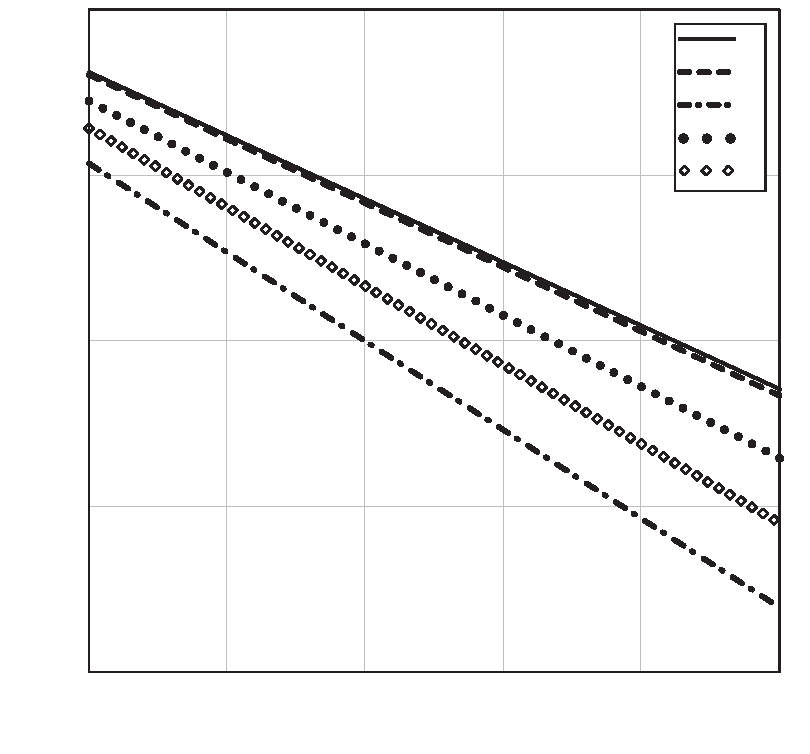
\includegraphics[width=\unitlength]{thermal_mismatch_stress_siavg}}%
        \put(0.09451188,0.05987052){\color[named]{black}\makebox(0,0)[lb]{\smash{200}}}%
        \put(0.26429042,0.05987052){\color[named]{black}\makebox(0,0)[lb]{\smash{250}}}%
        \put(0.43406896,0.05987052){\color[named]{black}\makebox(0,0)[lb]{\smash{300}}}%
        \put(0.60585397,0.05987052){\color[named]{black}\makebox(0,0)[lb]{\smash{350}}}%
        \put(0.77563251,0.05987052){\color[named]{black}\makebox(0,0)[lb]{\smash{400}}}%
        \put(0.94726318,0.05987052){\color[named]{black}\makebox(0,0)[lb]{\smash{450}}}%
        \put(0.10293962,0.28938027){\color[named]{black}\makebox(0,0)[rb]{\smash{$-$20}}}%
        \put(0.10402987,0.49388617){\color[named]{black}\makebox(0,0)[rb]{\smash{$-$15}}}%
        \put(0.10293962,0.69839215){\color[named]{black}\makebox(0,0)[rb]{\smash{$-$10}}}%
        \put(0.10402987,0.90289813){\color[named]{black}\makebox(0,0)[rb]{\smash{$-$5}}}%
        \put(0.92663254,0.870){\color[named]{black}\makebox(0,0)[b]{\smash{\textsl{1}}}}%
        \put(0.92663254,0.829){\color[named]{black}\makebox(0,0)[b]{\smash{\textsl{2}}}}%
        \put(0.92663254,0.789){\color[named]{black}\makebox(0,0)[b]{\smash{\textsl{3}}}}%
        \put(0.92663254,0.748){\color[named]{black}\makebox(0,0)[b]{\smash{\textsl{4}}}}%
        \put(0.92663254,0.708){\color[named]{black}\makebox(0,0)[b]{\smash{\textsl{5}}}}%
        \put(0.02500558,0.45122627){\color[named]{black}\rotatebox{90}{\makebox(0,0)[b]{\smash{$\sigma_{si}$, МПа}}}}%
        \put(0.10402987,0.08770316){\color[named]{black}\makebox(0,0)[rb]{\smash{$-$25}}}%
        \put(0.53641175,0.00777256){\color[named]{black}\makebox(0,0)[b]{\smash{$T_b$,~{\textdegree}C}}}%
      \end{picture}%
    \endgroup%

    \caption{Расчётная оценка остаточных напряжений по модели
    двух тонких слоёв в кремнии при температуре 20~{\textdegree}C
    в~зависимости от~температуры соединения с разными марками стекла
    (для расчёта взяты средние ТКЛР по~данным производителей):} % Этот
    % текст попадает в названия рисунков в списке рисунков
    \label{fig:thermal_mismatch_stress_siavg}
    \textsl{1} "--- Corning 7740,  \textsl{2} "--- Schott Borofloat 33,  \textsl{3} "--- ЛК5,  \textsl{4} "--- Hoya~SD\nobreakdash-2,  \textsl{5}~---~Asahi~SW\nobreakdash-YY%
\end{figure}
\begin{figure}[!htb]
    \centering
    \begingroup%
      \makeatletter%
      \providecommand\color[2][]{%
        \errmessage{(Inkscape) Color is used for the text in Inkscape, but the package 'color.sty' is not loaded}%
        \renewcommand\color[2][]{}%
      }%
      \providecommand\transparent[1]{%
        \errmessage{(Inkscape) Transparency is used (non-zero) for the text in Inkscape, but the package 'transparent.sty' is not loaded}%
        \renewcommand\transparent[1]{}%
      }%
      \providecommand\rotatebox[2]{#2}%
      \ifx\svgwidth\undefined%
        \setlength{\unitlength}{0.60\textwidth}%
        \ifx\svgscale\undefined%
          \relax%
        \else%
          \setlength{\unitlength}{\unitlength * \real{\svgscale}}%
        \fi%
      \else%
        \setlength{\unitlength}{\svgwidth}%
      \fi%
      \global\let\svgwidth\undefined%
      \global\let\svgscale\undefined%
      \makeatother%
      \begin{picture}(1,0.95586421)%
        \put(0,0){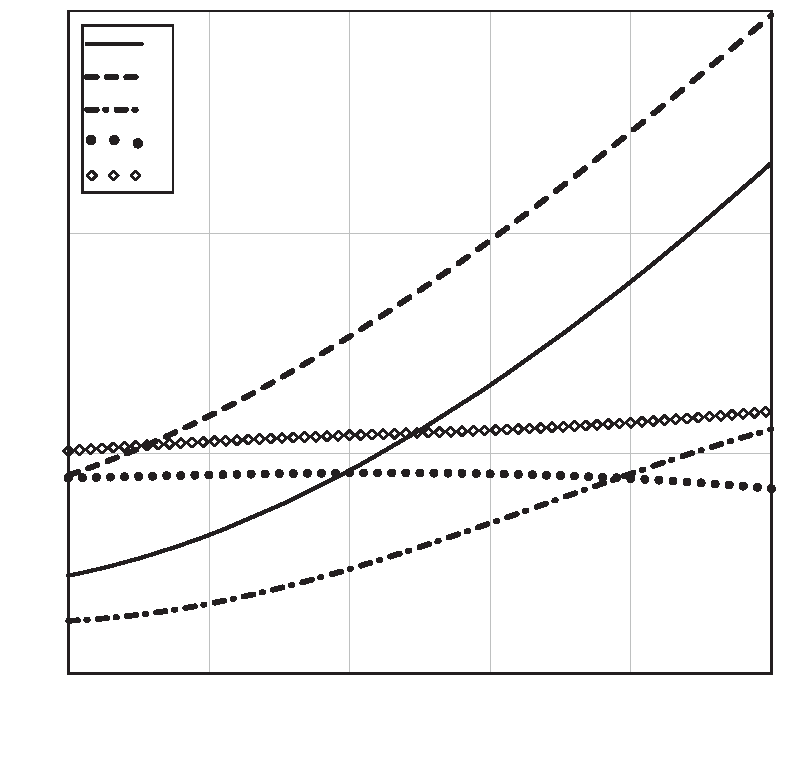
\includegraphics[width=\unitlength]{thermal_mismatch_stress_si}}%
        \put(0.07468862,0.37533739){\color[named]{black}\makebox(0,0)[rb]{\smash{0}}}%
        \put(0.07468862,0.65219154){\color[named]{black}\makebox(0,0)[rb]{\smash{5}}}%
        \put(0.07468862,0.9310884){\color[named]{black}\makebox(0,0)[rb]{\smash{10}}}%
        \put(0.19834598,0.89358804){\color[named]{black}\makebox(0,0)[b]{\smash{\textsl{1}}}}%
        \put(0.19834598,0.85226409){\color[named]{black}\makebox(0,0)[b]{\smash{\textsl{2}}}}%
        \put(0.19834598,0.81109742){\color[named]{black}\makebox(0,0)[b]{\smash{\textsl{3}}}}%
        \put(0.19834598,0.76977347){\color[named]{black}\makebox(0,0)[b]{\smash{\textsl{4}}}}%
        \put(0.19834598,0.7286068){\color[named]{black}\makebox(0,0)[b]{\smash{\textsl{5}}}}%
        \put(0.02545609,0.47127867){\color[named]{black}\rotatebox{90}{\makebox(0,0)[b]{\smash{$\sigma_{si}$, МПа}}}}%
        \put(0.07819749,0.06094908){\color[named]{black}\makebox(0,0)[lb]{\smash{200}}}%
        \put(0.25103498,0.06094908){\color[named]{black}\makebox(0,0)[lb]{\smash{250}}}%
        \put(0.42387246,0.06094908){\color[named]{black}\makebox(0,0)[lb]{\smash{300}}}%
        \put(0.59875257,0.06094908){\color[named]{black}\makebox(0,0)[lb]{\smash{350}}}%
        \put(0.77158998,0.06094908){\color[named]{black}\makebox(0,0)[lb]{\smash{400}}}%
        \put(0.94631305,0.06094908){\color[named]{black}\makebox(0,0)[lb]{\smash{450}}}%
        \put(0.52795474,0.00791253){\color[named]{black}\makebox(0,0)[b]{\smash{$T_b$,~{\textdegree}C}}}%
        \put(0.07468862,0.10330381){\color[named]{black}\makebox(0,0)[rb]{\smash{$-$5}}}%
      \end{picture}%
    \endgroup%

    \caption{Расчётная оценка остаточных напряжений по модели двух тонких слоёв в кремнии при температуре 20~{\textdegree}C в зависимости от~температуры соединения с разными марками стекла:}
    \label{fig:thermal_mismatch_stress_si}
    \textsl{1} "--- Corning 7740,  \textsl{2} "--- Schott Borofloat 33,  \textsl{3} "--- ЛК5,  \textsl{4} "--- Hoya~SD\nobreakdash-2,  \textsl{5}~---~Asahi~SW\nobreakdash-YY%
\end{figure}

Расчётная температура минимальных остаточных напряжений для Corning~7740 приведённая на Рисунке~\ref{fig:thermal_mismatch_stress_si} подтверждается экспериментальными данными из работы~\cite{LeeMC2005_gyro_siog}.

\begingroup
Иллюстрация, сравнивающая остаточные напряжения, рассчитанные по~средним значениям ТКЛР и рассчитанные по истинным значениям ТКЛР для модели многослойного композиционного материала, приведена
на~Рисунке~\ref{fig:tm_stress_si_compos_2fig_bf33_lk5}.\russianpar
\endgroup

\begin{figure}[!htbp]
    \centering
    \begingroup%
      \makeatletter%
      \providecommand\color[2][]{%
        \errmessage{(Inkscape) Color is used for the text in Inkscape, but the package 'color.sty' is not loaded}%
        \renewcommand\color[2][]{}%
      }%
      \providecommand\transparent[1]{%
        \errmessage{(Inkscape) Transparency is used (non-zero) for the text in Inkscape, but the package 'transparent.sty' is not loaded}%
        \renewcommand\transparent[1]{}%
      }%
      \providecommand\rotatebox[2]{#2}%
      \ifx\svgwidth\undefined%
        \setlength{\unitlength}{393.24069286bp}%
        \ifx\svgscale\undefined%
          \relax%
        \else%
          \setlength{\unitlength}{\unitlength * \real{\svgscale}}%
        \fi%
      \else%
        \setlength{\unitlength}{\svgwidth}%
      \fi%
      \global\let\svgwidth\undefined%
      \global\let\svgscale\undefined%
      \makeatother%
      \begin{picture}(1,0.57786925)(0,-0.04)%
        \put(0,0){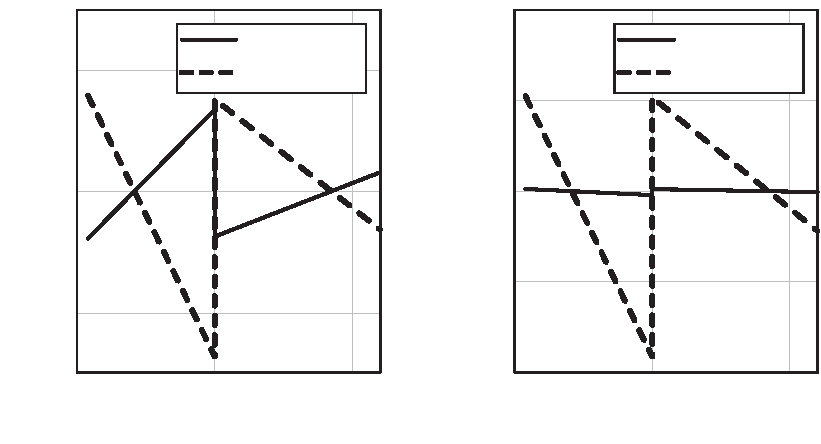
\includegraphics[width=\unitlength]{tm_stress_si_compos_2fig_bf33_lk5.pdf}}%
        \put(0.08193627,0.04661595){\color[named]{black}\makebox(0,0)[lb]{\smash{$-$0.5}}}%
        \put(0.26197873,0.04661588){\color[named]{black}\makebox(0,0)[lb]{\smash{0}}}%
        \put(0.41837149,0.04661588){\color[named]{black}\makebox(0,0)[lb]{\smash{0.5}}}%
        \put(0.08422509,0.14380795){\color[named]{black}\makebox(0,0)[rb]{\smash{$-$20}}}%
        \put(0.08422509,0.2925718){\color[named]{black}\makebox(0,0)[rb]{\smash{0}}}%
        \put(0.08422509,0.43950478){\color[named]{black}\makebox(0,0)[rb]{\smash{20}}}%
        \put(0.3001233,0.48146381){\color[named]{black}\makebox(0,0)[lb]{\smash{\small{Истинный}}}}%
        \put(0.3001233,0.44133571){\color[named]{black}\makebox(0,0)[lb]{\smash{{\small Средний}}}}%
        \put(0.27917176,0.00592778){\color[named]{black}\makebox(0,0)[b]{\smash{$z$, мм}}}%
        \put(0.02471946,0.30516171){\color[named]{black}\rotatebox{90}{\makebox(0,0)[b]{\smash{$\sigma_x^T$, МПа}}}}%
        \put(0.61596035,0.04661595){\color[named]{black}\makebox(0,0)[lb]{\smash{$-$0.5}}}%
        \put(0.79600281,0.04661588){\color[named]{black}\makebox(0,0)[lb]{\smash{0}}}%
        \put(0.95239558,0.04661588){\color[named]{black}\makebox(0,0)[lb]{\smash{0.5}}}%
        \put(0.61824917,0.18195252){\color[named]{black}\makebox(0,0)[rb]{\smash{$-$20}}}%
        \put(0.61824917,0.2925718){\color[named]{black}\makebox(0,0)[rb]{\smash{0}}}%
        \put(0.61824917,0.40319107){\color[named]{black}\makebox(0,0)[rb]{\smash{20}}}%
        \put(0.61824917,0.51381035){\color[named]{black}\makebox(0,0)[rb]{\smash{40}}}%
        \put(0.83414739,0.48146381){\color[named]{black}\makebox(0,0)[lb]{\small{Истинный}}}%
        \put(0.83414739,0.44133571){\color[named]{black}\makebox(0,0)[lb]{\smash{{\small Средний}}}}%
        \put(0.81319588,0.00592778){\color[named]{black}\makebox(0,0)[b]{\smash{$z$, мм}}}%
        \put(0.55874372,0.30516171){\color[named]{black}\rotatebox{90}{\makebox(0,0)[b]{\smash{$\sigma_x^T$, МПа}}}}%
        \put(0.61824917,0.07209782){\color[named]{black}\makebox(0,0)[rb]{\smash{$-$40}}}%
        \put(0.108,-0.04){%
        \fcolorbox{black}{siliconcolour}{\makebox[54pt]{Si}}%
        \fcolorbox{black}{glasscolour}{\makebox[74pt]{Borofloat 33}}%
        }%
        \put(0.64,-0.04){%
        \fcolorbox{black}{siliconcolour}{\makebox[55pt]{Si}}%
        \fcolorbox{black}{glasscolour}{\rule[1pt]{0pt}{7pt}\makebox[73pt]{ЛК5}}%
        }%
      \end{picture}%
    \endgroup%

    \caption{Расчётная оценка остаточных напряжений в~кремнии для двух стёкол (модель многослойного композиционного материала для истинных и~средних ТКЛР)
    при $T_w$ = 20~{\textdegree}C, $T_b$ = 400~{\textdegree}C}
    \label{fig:tm_stress_si_compos_2fig_bf33_lk5}
\end{figure}

%\clearpage
\subsection{Оценка вариации напряжений по модели двух тонких слоёв}
На Рисунке~\ref{fig:sigma_workt_bf33_lk5_simple} графиками показана расчётная
оценка по формуле~\eqref{eq:sigma_siupdated} остаточных напряжений в кремнии в
рабочем диапазоне температур (от~минус~60 до~85~{\textdegree}C) прибора при
разных фиксированных температурах $ T_b $ проведения процесса соединения со
стёклами марок Borofloat~33 и ЛК5. Расчёт проводился исходя из толщины кремния
460~мкм и толщины стекла 600~мкм.

\begin{figure}[htbp]
    \centering
    \ifdefmacro{\tikzsetnextfilename}{\tikzsetnextfilename{sigma_workt_bf33_lk5_simple}}{}%
    \begin{tikzpicture}[x=1pt,y=1pt]
\definecolor{fillColor}{RGB}{255,255,255}
\path[use as bounding box,fill=fillColor] (0,0) rectangle (483.70,227.34);
\begin{scope}
\path[clip] (  0.00,  0.00) rectangle (483.70,227.34);

\path[] (  0.00,  0.00) rectangle (483.70,227.34);
\end{scope}
\begin{scope}
\path[clip] (  0.00,  0.00) rectangle (241.85,227.34);
\definecolor{drawColor}{RGB}{255,255,255}
\definecolor{fillColor}{RGB}{255,255,255}

\path[draw=drawColor,line width= 0.6pt,line join=round,line cap=round,fill=fillColor] (  0.00,  0.00) rectangle (241.85,227.34);
\end{scope}
\begin{scope}
\path[clip] ( 40.77, 32.43) rectangle (237.63,217.40);
\definecolor{fillColor}{RGB}{255,255,255}

\path[fill=fillColor] ( 40.77, 32.43) rectangle (237.63,217.40);
\definecolor{drawColor}{gray}{0.98}

\path[draw=drawColor,line width= 0.6pt,line join=round] ( 40.77, 51.61) --
	(237.63, 51.61);

\path[draw=drawColor,line width= 0.6pt,line join=round] ( 40.77, 93.03) --
	(237.63, 93.03);

\path[draw=drawColor,line width= 0.6pt,line join=round] ( 40.77,134.44) --
	(237.63,134.44);

\path[draw=drawColor,line width= 0.6pt,line join=round] ( 40.77,175.86) --
	(237.63,175.86);

\path[draw=drawColor,line width= 0.6pt,line join=round] ( 40.77,217.28) --
	(237.63,217.28);

\path[draw=drawColor,line width= 0.6pt,line join=round] ( 74.40, 32.43) --
	( 74.40,217.40);

\path[draw=drawColor,line width= 0.6pt,line join=round] (111.43, 32.43) --
	(111.43,217.40);

\path[draw=drawColor,line width= 0.6pt,line join=round] (136.11, 32.43) --
	(136.11,217.40);

\path[draw=drawColor,line width= 0.6pt,line join=round] (173.14, 32.43) --
	(173.14,217.40);

\path[draw=drawColor,line width= 0.6pt,line join=round] (213.26, 32.43) --
	(213.26,217.40);
\definecolor{drawColor}{gray}{0.90}

\path[draw=drawColor,line width= 0.2pt,line join=round] ( 40.77, 72.32) --
	(237.63, 72.32);

\path[draw=drawColor,line width= 0.2pt,line join=round] ( 40.77,113.73) --
	(237.63,113.73);

\path[draw=drawColor,line width= 0.2pt,line join=round] ( 40.77,155.15) --
	(237.63,155.15);

\path[draw=drawColor,line width= 0.2pt,line join=round] ( 40.77,196.57) --
	(237.63,196.57);

\path[draw=drawColor,line width= 0.2pt,line join=round] ( 49.72, 32.43) --
	( 49.72,217.40);

\path[draw=drawColor,line width= 0.2pt,line join=round] ( 99.09, 32.43) --
	( 99.09,217.40);

\path[draw=drawColor,line width= 0.2pt,line join=round] (123.77, 32.43) --
	(123.77,217.40);

\path[draw=drawColor,line width= 0.2pt,line join=round] (148.46, 32.43) --
	(148.46,217.40);

\path[draw=drawColor,line width= 0.2pt,line join=round] (197.83, 32.43) --
	(197.83,217.40);

\path[draw=drawColor,line width= 0.2pt,line join=round] (228.68, 32.43) --
	(228.68,217.40);
\definecolor{drawColor}{RGB}{0,0,0}

\path[draw=drawColor,line width= 1.7pt,line join=round] ( 49.72,102.05) --
	( 51.50,102.89) --
	( 53.29,103.72) --
	( 55.08,104.54) --
	( 56.87,105.35) --
	( 58.66,106.15) --
	( 60.45,106.95) --
	( 62.24,107.73) --
	( 64.03,108.50) --
	( 65.82,109.27) --
	( 67.61,110.02) --
	( 69.40,110.77) --
	( 71.19,111.51) --
	( 72.98,112.24) --
	( 74.77,112.96) --
	( 76.56,113.67) --
	( 78.35,114.37) --
	( 80.14,115.07) --
	( 81.93,115.75) --
	( 83.72,116.43) --
	( 85.51,117.10) --
	( 87.30,117.76) --
	( 89.09,118.41) --
	( 90.88,119.06) --
	( 92.67,119.69) --
	( 94.46,120.32) --
	( 96.25,120.94) --
	( 98.04,121.55) --
	( 99.83,122.15) --
	(101.62,122.74) --
	(103.41,123.33) --
	(105.20,123.91) --
	(106.99,124.48) --
	(108.77,125.04) --
	(110.56,125.59) --
	(112.35,126.14) --
	(114.14,126.68) --
	(115.93,127.21) --
	(117.72,127.73) --
	(119.51,128.25) --
	(121.30,128.76) --
	(123.09,129.26) --
	(124.88,129.75) --
	(126.67,130.23) --
	(128.46,130.71) --
	(130.25,131.18) --
	(132.04,131.64) --
	(133.83,132.10) --
	(135.62,132.55) --
	(137.41,132.99) --
	(139.20,133.42) --
	(140.99,133.85) --
	(142.78,134.27) --
	(144.57,134.68) --
	(146.36,135.08) --
	(148.15,135.48) --
	(149.94,135.87) --
	(151.73,136.26) --
	(153.52,136.63) --
	(155.31,137.00) --
	(157.10,137.37) --
	(158.89,137.72) --
	(160.68,138.07) --
	(162.47,138.41) --
	(164.26,138.75) --
	(166.05,139.08) --
	(167.83,139.40) --
	(169.62,139.71) --
	(171.41,140.02) --
	(173.20,140.33) --
	(174.99,140.62) --
	(176.78,140.91) --
	(178.57,141.19) --
	(180.36,141.47) --
	(182.15,141.74) --
	(183.94,142.00) --
	(185.73,142.26) --
	(187.52,142.51) --
	(189.31,142.76) --
	(191.10,142.99) --
	(192.89,143.23) --
	(194.68,143.45) --
	(196.47,143.67) --
	(198.26,143.89) --
	(200.05,144.09) --
	(201.84,144.29) --
	(203.63,144.49) --
	(205.42,144.68) --
	(207.21,144.86) --
	(209.00,145.04) --
	(210.79,145.21) --
	(212.58,145.38) --
	(214.37,145.54) --
	(216.16,145.69) --
	(217.95,145.84) --
	(219.74,145.98) --
	(221.53,146.12) --
	(223.32,146.25) --
	(225.10,146.37) --
	(226.89,146.49) --
	(228.68,146.60);

\path[draw=drawColor,line width= 1.7pt,dash pattern=on 2pt off 2pt ,line join=round] ( 49.72,130.02) --
	( 51.50,130.85) --
	( 53.29,131.68) --
	( 55.08,132.50) --
	( 56.87,133.31) --
	( 58.66,134.12) --
	( 60.45,134.91) --
	( 62.24,135.69) --
	( 64.03,136.46) --
	( 65.82,137.23) --
	( 67.61,137.99) --
	( 69.40,138.73) --
	( 71.19,139.47) --
	( 72.98,140.20) --
	( 74.77,140.92) --
	( 76.56,141.63) --
	( 78.35,142.34) --
	( 80.14,143.03) --
	( 81.93,143.72) --
	( 83.72,144.39) --
	( 85.51,145.06) --
	( 87.30,145.72) --
	( 89.09,146.37) --
	( 90.88,147.02) --
	( 92.67,147.65) --
	( 94.46,148.28) --
	( 96.25,148.90) --
	( 98.04,149.51) --
	( 99.83,150.11) --
	(101.62,150.71) --
	(103.41,151.29) --
	(105.20,151.87) --
	(106.99,152.44) --
	(108.77,153.00) --
	(110.56,153.56) --
	(112.35,154.10) --
	(114.14,154.64) --
	(115.93,155.17) --
	(117.72,155.69) --
	(119.51,156.21) --
	(121.30,156.72) --
	(123.09,157.22) --
	(124.88,157.71) --
	(126.67,158.20) --
	(128.46,158.67) --
	(130.25,159.14) --
	(132.04,159.61) --
	(133.83,160.06) --
	(135.62,160.51) --
	(137.41,160.95) --
	(139.20,161.38) --
	(140.99,161.81) --
	(142.78,162.23) --
	(144.57,162.64) --
	(146.36,163.05) --
	(148.15,163.44) --
	(149.94,163.83) --
	(151.73,164.22) --
	(153.52,164.59) --
	(155.31,164.96) --
	(157.10,165.33) --
	(158.89,165.68) --
	(160.68,166.03) --
	(162.47,166.37) --
	(164.26,166.71) --
	(166.05,167.04) --
	(167.83,167.36) --
	(169.62,167.68) --
	(171.41,167.99) --
	(173.20,168.29) --
	(174.99,168.58) --
	(176.78,168.87) --
	(178.57,169.16) --
	(180.36,169.43) --
	(182.15,169.70) --
	(183.94,169.97) --
	(185.73,170.22) --
	(187.52,170.47) --
	(189.31,170.72) --
	(191.10,170.96) --
	(192.89,171.19) --
	(194.68,171.41) --
	(196.47,171.63) --
	(198.26,171.85) --
	(200.05,172.05) --
	(201.84,172.26) --
	(203.63,172.45) --
	(205.42,172.64) --
	(207.21,172.82) --
	(209.00,173.00) --
	(210.79,173.17) --
	(212.58,173.34) --
	(214.37,173.50) --
	(216.16,173.65) --
	(217.95,173.80) --
	(219.74,173.94) --
	(221.53,174.08) --
	(223.32,174.21) --
	(225.10,174.33) --
	(226.89,174.45) --
	(228.68,174.57);

\path[draw=drawColor,line width= 1.7pt,dash pattern=on 4pt off 2pt ,line join=round] ( 49.72,162.31) --
	( 51.50,163.15) --
	( 53.29,163.98) --
	( 55.08,164.80) --
	( 56.87,165.61) --
	( 58.66,166.41) --
	( 60.45,167.20) --
	( 62.24,167.99) --
	( 64.03,168.76) --
	( 65.82,169.53) --
	( 67.61,170.28) --
	( 69.40,171.03) --
	( 71.19,171.77) --
	( 72.98,172.50) --
	( 74.77,173.22) --
	( 76.56,173.93) --
	( 78.35,174.63) --
	( 80.14,175.33) --
	( 81.93,176.01) --
	( 83.72,176.69) --
	( 85.51,177.36) --
	( 87.30,178.02) --
	( 89.09,178.67) --
	( 90.88,179.31) --
	( 92.67,179.95) --
	( 94.46,180.58) --
	( 96.25,181.19) --
	( 98.04,181.81) --
	( 99.83,182.41) --
	(101.62,183.00) --
	(103.41,183.59) --
	(105.20,184.17) --
	(106.99,184.74) --
	(108.77,185.30) --
	(110.56,185.85) --
	(112.35,186.40) --
	(114.14,186.94) --
	(115.93,187.47) --
	(117.72,187.99) --
	(119.51,188.51) --
	(121.30,189.01) --
	(123.09,189.52) --
	(124.88,190.01) --
	(126.67,190.49) --
	(128.46,190.97) --
	(130.25,191.44) --
	(132.04,191.90) --
	(133.83,192.36) --
	(135.62,192.81) --
	(137.41,193.25) --
	(139.20,193.68) --
	(140.99,194.11) --
	(142.78,194.53) --
	(144.57,194.94) --
	(146.36,195.34) --
	(148.15,195.74) --
	(149.94,196.13) --
	(151.73,196.51) --
	(153.52,196.89) --
	(155.31,197.26) --
	(157.10,197.62) --
	(158.89,197.98) --
	(160.68,198.33) --
	(162.47,198.67) --
	(164.26,199.01) --
	(166.05,199.34) --
	(167.83,199.66) --
	(169.62,199.97) --
	(171.41,200.28) --
	(173.20,200.58) --
	(174.99,200.88) --
	(176.78,201.17) --
	(178.57,201.45) --
	(180.36,201.73) --
	(182.15,202.00) --
	(183.94,202.26) --
	(185.73,202.52) --
	(187.52,202.77) --
	(189.31,203.01) --
	(191.10,203.25) --
	(192.89,203.48) --
	(194.68,203.71) --
	(196.47,203.93) --
	(198.26,204.14) --
	(200.05,204.35) --
	(201.84,204.55) --
	(203.63,204.75) --
	(205.42,204.94) --
	(207.21,205.12) --
	(209.00,205.30) --
	(210.79,205.47) --
	(212.58,205.63) --
	(214.37,205.79) --
	(216.16,205.95) --
	(217.95,206.10) --
	(219.74,206.24) --
	(221.53,206.37) --
	(223.32,206.50) --
	(225.10,206.63) --
	(226.89,206.75) --
	(228.68,206.86);

\path[draw=drawColor,line width= 0.9pt,line join=round,line cap=round] ( 40.77, 32.43) rectangle (237.63,217.40);
\end{scope}
\begin{scope}
\path[clip] (  0.00,  0.00) rectangle (483.70,227.34);
\definecolor{drawColor}{RGB}{0,0,0}

\node[text=drawColor,anchor=base east,inner sep=0pt, outer sep=0pt, scale=  1.00] at ( 35.37, 67.36) {\(-5\)};

\node[text=drawColor,anchor=base east,inner sep=0pt, outer sep=0pt, scale=  1.00] at ( 35.37,108.78) {\(0\)};

\node[text=drawColor,anchor=base east,inner sep=0pt, outer sep=0pt, scale=  1.00] at ( 35.37,150.19) {\(5\)};

\node[text=drawColor,anchor=base east,inner sep=0pt, outer sep=0pt, scale=  1.00] at ( 35.37,191.61) {\(10\)};
\end{scope}
\begin{scope}
\path[clip] (  0.00,  0.00) rectangle (483.70,227.34);
\definecolor{drawColor}{RGB}{0,0,0}

\path[draw=drawColor,line width= 0.6pt,line join=round] ( 37.77, 72.32) --
	( 40.77, 72.32);

\path[draw=drawColor,line width= 0.6pt,line join=round] ( 37.77,113.73) --
	( 40.77,113.73);

\path[draw=drawColor,line width= 0.6pt,line join=round] ( 37.77,155.15) --
	( 40.77,155.15);

\path[draw=drawColor,line width= 0.6pt,line join=round] ( 37.77,196.57) --
	( 40.77,196.57);
\end{scope}
\begin{scope}
\path[clip] (  0.00,  0.00) rectangle (483.70,227.34);
\definecolor{drawColor}{RGB}{0,0,0}

\path[draw=drawColor,line width= 0.6pt,line join=round] ( 49.72, 29.43) --
	( 49.72, 32.43);

\path[draw=drawColor,line width= 0.6pt,line join=round] ( 99.09, 29.43) --
	( 99.09, 32.43);

\path[draw=drawColor,line width= 0.6pt,line join=round] (123.77, 29.43) --
	(123.77, 32.43);

\path[draw=drawColor,line width= 0.6pt,line join=round] (148.46, 29.43) --
	(148.46, 32.43);

\path[draw=drawColor,line width= 0.6pt,line join=round] (197.83, 29.43) --
	(197.83, 32.43);

\path[draw=drawColor,line width= 0.6pt,line join=round] (228.68, 29.43) --
	(228.68, 32.43);
\end{scope}
\begin{scope}
\path[clip] (  0.00,  0.00) rectangle (483.70,227.34);
\definecolor{drawColor}{RGB}{0,0,0}

\node[text=drawColor,anchor=base,inner sep=0pt, outer sep=0pt, scale=  1.00] at ( 49.72, 17.12) {\(-60\)};

\node[text=drawColor,anchor=base,inner sep=0pt, outer sep=0pt, scale=  1.00] at ( 99.09, 17.12) {\(-20\)};

\node[text=drawColor,anchor=base,inner sep=0pt, outer sep=0pt, scale=  1.00] at (123.77, 17.12) {\(0\)};

\node[text=drawColor,anchor=base,inner sep=0pt, outer sep=0pt, scale=  1.00] at (148.46, 17.12) {\(20\)};

\node[text=drawColor,anchor=base,inner sep=0pt, outer sep=0pt, scale=  1.00] at (197.83, 17.12) {\(60\)};

\node[text=drawColor,anchor=base,inner sep=0pt, outer sep=0pt, scale=  1.00] at (228.68, 17.12) {\(85\)};
\end{scope}
\begin{scope}
\path[clip] (  0.00,  0.00) rectangle (483.70,227.34);
\definecolor{drawColor}{RGB}{0,0,0}

\node[text=drawColor,anchor=base,inner sep=0pt, outer sep=0pt, scale=  1.00] at (139.20,  2.40) {Tемпература, \({}^\circ\)C};
\end{scope}
\begin{scope}
\path[clip] (  0.00,  0.00) rectangle (483.70,227.34);
\definecolor{drawColor}{RGB}{0,0,0}

\node[text=drawColor,rotate= 90.00,anchor=base,inner sep=0pt, outer sep=0pt, scale=  1.00] at ( 12.32,124.92) {\(\sigma_{si}\), МПа};
\end{scope}
\begin{scope}
\path[clip] (  0.00,  0.00) rectangle (483.70,227.34);
\definecolor{drawColor}{RGB}{0,0,0}
\definecolor{fillColor}{RGB}{255,255,255}

\path[draw=drawColor,line width= 0.6pt,line join=round,line cap=round,fill=fillColor] (129.31, 36.13) rectangle (233.70,100.12);
\end{scope}
\begin{scope}
\path[clip] (  0.00,  0.00) rectangle (483.70,227.34);
\definecolor{drawColor}{RGB}{0,0,0}

\node[text=drawColor,anchor=base west,inner sep=0pt, outer sep=0pt, scale=  1.00] at (133.58, 85.93) {Соединено при:\hspace*{1.3em}};
\end{scope}
\begin{scope}
\path[clip] (  0.00,  0.00) rectangle (483.70,227.34);
\definecolor{drawColor}{RGB}{255,255,255}
\definecolor{fillColor}{RGB}{255,255,255}

\path[draw=drawColor,line width= 0.6pt,line join=round,line cap=round,fill=fillColor] (133.58, 67.38) rectangle (160.56, 80.87);
\end{scope}
\begin{scope}
\path[clip] (  0.00,  0.00) rectangle (483.70,227.34);
\definecolor{drawColor}{RGB}{0,0,0}

\path[draw=drawColor,line width= 1.7pt,line join=round] (136.27, 74.13) -- (157.86, 74.13);
\end{scope}
\begin{scope}
\path[clip] (  0.00,  0.00) rectangle (483.70,227.34);
\definecolor{drawColor}{RGB}{0,0,0}

\path[draw=drawColor,line width= 1.7pt,line join=round] (136.27, 74.13) -- (157.86, 74.13);
\end{scope}
\begin{scope}
\path[clip] (  0.00,  0.00) rectangle (483.70,227.34);
\definecolor{drawColor}{RGB}{0,0,0}

\path[draw=drawColor,line width= 1.7pt,line join=round] (136.27, 74.13) -- (157.86, 74.13);
\end{scope}
\begin{scope}
\path[clip] (  0.00,  0.00) rectangle (483.70,227.34);
\definecolor{drawColor}{RGB}{255,255,255}
\definecolor{fillColor}{RGB}{255,255,255}

\path[draw=drawColor,line width= 0.6pt,line join=round,line cap=round,fill=fillColor] (133.58, 53.89) rectangle (160.56, 67.38);
\end{scope}
\begin{scope}
\path[clip] (  0.00,  0.00) rectangle (483.70,227.34);
\definecolor{drawColor}{RGB}{0,0,0}

\path[draw=drawColor,line width= 1.7pt,dash pattern=on 2pt off 2pt ,line join=round] (136.27, 60.64) -- (157.86, 60.64);
\end{scope}
\begin{scope}
\path[clip] (  0.00,  0.00) rectangle (483.70,227.34);
\definecolor{drawColor}{RGB}{0,0,0}

\path[draw=drawColor,line width= 1.7pt,dash pattern=on 2pt off 2pt ,line join=round] (136.27, 60.64) -- (157.86, 60.64);
\end{scope}
\begin{scope}
\path[clip] (  0.00,  0.00) rectangle (483.70,227.34);
\definecolor{drawColor}{RGB}{0,0,0}

\path[draw=drawColor,line width= 1.7pt,dash pattern=on 2pt off 2pt ,line join=round] (136.27, 60.64) -- (157.86, 60.64);
\end{scope}
\begin{scope}
\path[clip] (  0.00,  0.00) rectangle (483.70,227.34);
\definecolor{drawColor}{RGB}{255,255,255}
\definecolor{fillColor}{RGB}{255,255,255}

\path[draw=drawColor,line width= 0.6pt,line join=round,line cap=round,fill=fillColor] (133.58, 40.40) rectangle (160.56, 53.89);
\end{scope}
\begin{scope}
\path[clip] (  0.00,  0.00) rectangle (483.70,227.34);
\definecolor{drawColor}{RGB}{0,0,0}

\path[draw=drawColor,line width= 1.7pt,dash pattern=on 4pt off 2pt ,line join=round] (136.27, 47.15) -- (157.86, 47.15);
\end{scope}
\begin{scope}
\path[clip] (  0.00,  0.00) rectangle (483.70,227.34);
\definecolor{drawColor}{RGB}{0,0,0}

\path[draw=drawColor,line width= 1.7pt,dash pattern=on 4pt off 2pt ,line join=round] (136.27, 47.15) -- (157.86, 47.15);
\end{scope}
\begin{scope}
\path[clip] (  0.00,  0.00) rectangle (483.70,227.34);
\definecolor{drawColor}{RGB}{0,0,0}

\path[draw=drawColor,line width= 1.7pt,dash pattern=on 4pt off 2pt ,line join=round] (136.27, 47.15) -- (157.86, 47.15);
\end{scope}
\begin{scope}
\path[clip] (  0.00,  0.00) rectangle (483.70,227.34);
\definecolor{drawColor}{RGB}{0,0,0}

\node[text=drawColor,anchor=base east,inner sep=0pt, outer sep=0pt, scale=  1.00] at (203.62, 69.17) {300 \({}^\circ\)C};
\end{scope}
\begin{scope}
\path[clip] (  0.00,  0.00) rectangle (483.70,227.34);
\definecolor{drawColor}{RGB}{0,0,0}

\node[text=drawColor,anchor=base east,inner sep=0pt, outer sep=0pt, scale=  1.00] at (203.62, 55.68) {375 \({}^\circ\)C};
\end{scope}
\begin{scope}
\path[clip] (  0.00,  0.00) rectangle (483.70,227.34);
\definecolor{drawColor}{RGB}{0,0,0}

\node[text=drawColor,anchor=base east,inner sep=0pt, outer sep=0pt, scale=  1.00] at (203.62, 42.19) {450 \({}^\circ\)C};
\end{scope}
\begin{scope}
\path[clip] (  0.00,  0.00) rectangle (483.70,227.34);
\definecolor{drawColor}{RGB}{0,0,0}

\node[text=drawColor,anchor=base west,inner sep=0pt, outer sep=0pt, scale=  1.00] at ( 43.00,202.22) {\bfseries Borofloat 33};
\end{scope}
\begin{scope}
\path[clip] (241.85,  0.00) rectangle (483.70,227.34);
\definecolor{drawColor}{RGB}{255,255,255}
\definecolor{fillColor}{RGB}{255,255,255}

\path[draw=drawColor,line width= 0.6pt,line join=round,line cap=round,fill=fillColor] (241.85,  0.00) rectangle (483.70,227.34);
\end{scope}
\begin{scope}
\path[clip] (282.62, 32.43) rectangle (479.48,217.40);
\definecolor{fillColor}{RGB}{255,255,255}

\path[fill=fillColor] (282.62, 32.43) rectangle (479.48,217.40);
\definecolor{drawColor}{gray}{0.98}

\path[draw=drawColor,line width= 0.6pt,line join=round] (282.62, 51.61) --
	(479.48, 51.61);

\path[draw=drawColor,line width= 0.6pt,line join=round] (282.62, 93.03) --
	(479.48, 93.03);

\path[draw=drawColor,line width= 0.6pt,line join=round] (282.62,134.44) --
	(479.48,134.44);

\path[draw=drawColor,line width= 0.6pt,line join=round] (282.62,175.86) --
	(479.48,175.86);

\path[draw=drawColor,line width= 0.6pt,line join=round] (282.62,217.28) --
	(479.48,217.28);

\path[draw=drawColor,line width= 0.6pt,line join=round] (316.25, 32.43) --
	(316.25,217.40);

\path[draw=drawColor,line width= 0.6pt,line join=round] (353.28, 32.43) --
	(353.28,217.40);

\path[draw=drawColor,line width= 0.6pt,line join=round] (377.96, 32.43) --
	(377.96,217.40);

\path[draw=drawColor,line width= 0.6pt,line join=round] (414.99, 32.43) --
	(414.99,217.40);

\path[draw=drawColor,line width= 0.6pt,line join=round] (455.10, 32.43) --
	(455.10,217.40);
\definecolor{drawColor}{gray}{0.90}

\path[draw=drawColor,line width= 0.2pt,line join=round] (282.62, 72.32) --
	(479.48, 72.32);

\path[draw=drawColor,line width= 0.2pt,line join=round] (282.62,113.73) --
	(479.48,113.73);

\path[draw=drawColor,line width= 0.2pt,line join=round] (282.62,155.15) --
	(479.48,155.15);

\path[draw=drawColor,line width= 0.2pt,line join=round] (282.62,196.57) --
	(479.48,196.57);

\path[draw=drawColor,line width= 0.2pt,line join=round] (291.56, 32.43) --
	(291.56,217.40);

\path[draw=drawColor,line width= 0.2pt,line join=round] (340.93, 32.43) --
	(340.93,217.40);

\path[draw=drawColor,line width= 0.2pt,line join=round] (365.62, 32.43) --
	(365.62,217.40);

\path[draw=drawColor,line width= 0.2pt,line join=round] (390.31, 32.43) --
	(390.31,217.40);

\path[draw=drawColor,line width= 0.2pt,line join=round] (439.68, 32.43) --
	(439.68,217.40);

\path[draw=drawColor,line width= 0.2pt,line join=round] (470.53, 32.43) --
	(470.53,217.40);
\definecolor{drawColor}{RGB}{0,0,0}

\path[draw=drawColor,line width= 1.7pt,line join=round] (291.56, 47.77) --
	(293.35, 48.78) --
	(295.14, 49.78) --
	(296.93, 50.78) --
	(298.72, 51.76) --
	(300.51, 52.74) --
	(302.30, 53.71) --
	(304.09, 54.67) --
	(305.88, 55.62) --
	(307.67, 56.57) --
	(309.46, 57.51) --
	(311.25, 58.43) --
	(313.04, 59.35) --
	(314.83, 60.27) --
	(316.62, 61.17) --
	(318.41, 62.07) --
	(320.20, 62.96) --
	(321.99, 63.84) --
	(323.78, 64.71) --
	(325.57, 65.58) --
	(327.36, 66.44) --
	(329.15, 67.29) --
	(330.94, 68.13) --
	(332.73, 68.96) --
	(334.52, 69.79) --
	(336.31, 70.61) --
	(338.10, 71.42) --
	(339.89, 72.23) --
	(341.67, 73.02) --
	(343.46, 73.81) --
	(345.25, 74.60) --
	(347.04, 75.37) --
	(348.83, 76.14) --
	(350.62, 76.90) --
	(352.41, 77.65) --
	(354.20, 78.40) --
	(355.99, 79.14) --
	(357.78, 79.87) --
	(359.57, 80.59) --
	(361.36, 81.31) --
	(363.15, 82.02) --
	(364.94, 82.72) --
	(366.73, 83.42) --
	(368.52, 84.11) --
	(370.31, 84.79) --
	(372.10, 85.46) --
	(373.89, 86.13) --
	(375.68, 86.79) --
	(377.47, 87.44) --
	(379.26, 88.09) --
	(381.05, 88.73) --
	(382.84, 89.37) --
	(384.63, 89.99) --
	(386.42, 90.61) --
	(388.21, 91.23) --
	(390.00, 91.83) --
	(391.79, 92.43) --
	(393.58, 93.03) --
	(395.37, 93.61) --
	(397.16, 94.19) --
	(398.95, 94.77) --
	(400.73, 95.34) --
	(402.52, 95.90) --
	(404.31, 96.45) --
	(406.10, 97.00) --
	(407.89, 97.54) --
	(409.68, 98.07) --
	(411.47, 98.60) --
	(413.26, 99.13) --
	(415.05, 99.64) --
	(416.84,100.15) --
	(418.63,100.66) --
	(420.42,101.15) --
	(422.21,101.64) --
	(424.00,102.13) --
	(425.79,102.61) --
	(427.58,103.08) --
	(429.37,103.55) --
	(431.16,104.01) --
	(432.95,104.46) --
	(434.74,104.91) --
	(436.53,105.35) --
	(438.32,105.79) --
	(440.11,106.22) --
	(441.90,106.64) --
	(443.69,107.06) --
	(445.48,107.48) --
	(447.27,107.88) --
	(449.06,108.28) --
	(450.85,108.68) --
	(452.64,109.07) --
	(454.43,109.45) --
	(456.22,109.83) --
	(458.00,110.20) --
	(459.79,110.57) --
	(461.58,110.93) --
	(463.37,111.29) --
	(465.16,111.64) --
	(466.95,111.98) --
	(468.74,112.32) --
	(470.53,112.65);

\path[draw=drawColor,line width= 1.7pt,dash pattern=on 2pt off 2pt ,line join=round] (291.56, 61.02) --
	(293.35, 62.03) --
	(295.14, 63.03) --
	(296.93, 64.02) --
	(298.72, 65.01) --
	(300.51, 65.99) --
	(302.30, 66.96) --
	(304.09, 67.92) --
	(305.88, 68.87) --
	(307.67, 69.81) --
	(309.46, 70.75) --
	(311.25, 71.68) --
	(313.04, 72.60) --
	(314.83, 73.51) --
	(316.62, 74.42) --
	(318.41, 75.31) --
	(320.20, 76.20) --
	(321.99, 77.08) --
	(323.78, 77.96) --
	(325.57, 78.82) --
	(327.36, 79.68) --
	(329.15, 80.53) --
	(330.94, 81.37) --
	(332.73, 82.21) --
	(334.52, 83.04) --
	(336.31, 83.86) --
	(338.10, 84.67) --
	(339.89, 85.47) --
	(341.67, 86.27) --
	(343.46, 87.06) --
	(345.25, 87.84) --
	(347.04, 88.62) --
	(348.83, 89.38) --
	(350.62, 90.14) --
	(352.41, 90.90) --
	(354.20, 91.64) --
	(355.99, 92.38) --
	(357.78, 93.11) --
	(359.57, 93.84) --
	(361.36, 94.55) --
	(363.15, 95.26) --
	(364.94, 95.97) --
	(366.73, 96.66) --
	(368.52, 97.35) --
	(370.31, 98.03) --
	(372.10, 98.71) --
	(373.89, 99.38) --
	(375.68,100.04) --
	(377.47,100.69) --
	(379.26,101.34) --
	(381.05,101.98) --
	(382.84,102.61) --
	(384.63,103.24) --
	(386.42,103.86) --
	(388.21,104.47) --
	(390.00,105.08) --
	(391.79,105.68) --
	(393.58,106.27) --
	(395.37,106.86) --
	(397.16,107.44) --
	(398.95,108.01) --
	(400.73,108.58) --
	(402.52,109.14) --
	(404.31,109.70) --
	(406.10,110.24) --
	(407.89,110.79) --
	(409.68,111.32) --
	(411.47,111.85) --
	(413.26,112.37) --
	(415.05,112.89) --
	(416.84,113.40) --
	(418.63,113.90) --
	(420.42,114.40) --
	(422.21,114.89) --
	(424.00,115.37) --
	(425.79,115.85) --
	(427.58,116.33) --
	(429.37,116.79) --
	(431.16,117.25) --
	(432.95,117.71) --
	(434.74,118.16) --
	(436.53,118.60) --
	(438.32,119.04) --
	(440.11,119.47) --
	(441.90,119.89) --
	(443.69,120.31) --
	(445.48,120.72) --
	(447.27,121.13) --
	(449.06,121.53) --
	(450.85,121.92) --
	(452.64,122.31) --
	(454.43,122.70) --
	(456.22,123.08) --
	(458.00,123.45) --
	(459.79,123.82) --
	(461.58,124.18) --
	(463.37,124.53) --
	(465.16,124.88) --
	(466.95,125.23) --
	(468.74,125.56) --
	(470.53,125.90);

\path[draw=drawColor,line width= 1.7pt,dash pattern=on 4pt off 2pt ,line join=round] (291.56, 73.98) --
	(293.35, 74.99) --
	(295.14, 75.99) --
	(296.93, 76.98) --
	(298.72, 77.97) --
	(300.51, 78.94) --
	(302.30, 79.91) --
	(304.09, 80.88) --
	(305.88, 81.83) --
	(307.67, 82.77) --
	(309.46, 83.71) --
	(311.25, 84.64) --
	(313.04, 85.56) --
	(314.83, 86.47) --
	(316.62, 87.38) --
	(318.41, 88.27) --
	(320.20, 89.16) --
	(321.99, 90.04) --
	(323.78, 90.92) --
	(325.57, 91.78) --
	(327.36, 92.64) --
	(329.15, 93.49) --
	(330.94, 94.33) --
	(332.73, 95.17) --
	(334.52, 95.99) --
	(336.31, 96.81) --
	(338.10, 97.63) --
	(339.89, 98.43) --
	(341.67, 99.23) --
	(343.46,100.02) --
	(345.25,100.80) --
	(347.04,101.57) --
	(348.83,102.34) --
	(350.62,103.10) --
	(352.41,103.86) --
	(354.20,104.60) --
	(355.99,105.34) --
	(357.78,106.07) --
	(359.57,106.79) --
	(361.36,107.51) --
	(363.15,108.22) --
	(364.94,108.92) --
	(366.73,109.62) --
	(368.52,110.31) --
	(370.31,110.99) --
	(372.10,111.67) --
	(373.89,112.33) --
	(375.68,112.99) --
	(377.47,113.65) --
	(379.26,114.30) --
	(381.05,114.94) --
	(382.84,115.57) --
	(384.63,116.20) --
	(386.42,116.82) --
	(388.21,117.43) --
	(390.00,118.04) --
	(391.79,118.64) --
	(393.58,119.23) --
	(395.37,119.82) --
	(397.16,120.40) --
	(398.95,120.97) --
	(400.73,121.54) --
	(402.52,122.10) --
	(404.31,122.65) --
	(406.10,123.20) --
	(407.89,123.74) --
	(409.68,124.28) --
	(411.47,124.81) --
	(413.26,125.33) --
	(415.05,125.85) --
	(416.84,126.36) --
	(418.63,126.86) --
	(420.42,127.36) --
	(422.21,127.85) --
	(424.00,128.33) --
	(425.79,128.81) --
	(427.58,129.28) --
	(429.37,129.75) --
	(431.16,130.21) --
	(432.95,130.67) --
	(434.74,131.11) --
	(436.53,131.56) --
	(438.32,131.99) --
	(440.11,132.42) --
	(441.90,132.85) --
	(443.69,133.27) --
	(445.48,133.68) --
	(447.27,134.09) --
	(449.06,134.49) --
	(450.85,134.88) --
	(452.64,135.27) --
	(454.43,135.66) --
	(456.22,136.03) --
	(458.00,136.41) --
	(459.79,136.77) --
	(461.58,137.13) --
	(463.37,137.49) --
	(465.16,137.84) --
	(466.95,138.18) --
	(468.74,138.52) --
	(470.53,138.86);

\path[draw=drawColor,line width= 0.9pt,line join=round,line cap=round] (282.62, 32.43) rectangle (479.48,217.40);
\end{scope}
\begin{scope}
\path[clip] (  0.00,  0.00) rectangle (483.70,227.34);
\definecolor{drawColor}{RGB}{0,0,0}

\node[text=drawColor,anchor=base east,inner sep=0pt, outer sep=0pt, scale=  1.00] at (277.22, 67.36) {\(-5\)};

\node[text=drawColor,anchor=base east,inner sep=0pt, outer sep=0pt, scale=  1.00] at (277.22,108.78) {\(0\)};

\node[text=drawColor,anchor=base east,inner sep=0pt, outer sep=0pt, scale=  1.00] at (277.22,150.19) {\(5\)};

\node[text=drawColor,anchor=base east,inner sep=0pt, outer sep=0pt, scale=  1.00] at (277.22,191.61) {\(10\)};
\end{scope}
\begin{scope}
\path[clip] (  0.00,  0.00) rectangle (483.70,227.34);
\definecolor{drawColor}{RGB}{0,0,0}

\path[draw=drawColor,line width= 0.6pt,line join=round] (279.62, 72.32) --
	(282.62, 72.32);

\path[draw=drawColor,line width= 0.6pt,line join=round] (279.62,113.73) --
	(282.62,113.73);

\path[draw=drawColor,line width= 0.6pt,line join=round] (279.62,155.15) --
	(282.62,155.15);

\path[draw=drawColor,line width= 0.6pt,line join=round] (279.62,196.57) --
	(282.62,196.57);
\end{scope}
\begin{scope}
\path[clip] (  0.00,  0.00) rectangle (483.70,227.34);
\definecolor{drawColor}{RGB}{0,0,0}

\path[draw=drawColor,line width= 0.6pt,line join=round] (291.56, 29.43) --
	(291.56, 32.43);

\path[draw=drawColor,line width= 0.6pt,line join=round] (340.93, 29.43) --
	(340.93, 32.43);

\path[draw=drawColor,line width= 0.6pt,line join=round] (365.62, 29.43) --
	(365.62, 32.43);

\path[draw=drawColor,line width= 0.6pt,line join=round] (390.31, 29.43) --
	(390.31, 32.43);

\path[draw=drawColor,line width= 0.6pt,line join=round] (439.68, 29.43) --
	(439.68, 32.43);

\path[draw=drawColor,line width= 0.6pt,line join=round] (470.53, 29.43) --
	(470.53, 32.43);
\end{scope}
\begin{scope}
\path[clip] (  0.00,  0.00) rectangle (483.70,227.34);
\definecolor{drawColor}{RGB}{0,0,0}

\node[text=drawColor,anchor=base,inner sep=0pt, outer sep=0pt, scale=  1.00] at (291.56, 17.12) {\(-60\)};

\node[text=drawColor,anchor=base,inner sep=0pt, outer sep=0pt, scale=  1.00] at (340.93, 17.12) {\(-20\)};

\node[text=drawColor,anchor=base,inner sep=0pt, outer sep=0pt, scale=  1.00] at (365.62, 17.12) {\(0\)};

\node[text=drawColor,anchor=base,inner sep=0pt, outer sep=0pt, scale=  1.00] at (390.31, 17.12) {\(20\)};

\node[text=drawColor,anchor=base,inner sep=0pt, outer sep=0pt, scale=  1.00] at (439.68, 17.12) {\(60\)};

\node[text=drawColor,anchor=base,inner sep=0pt, outer sep=0pt, scale=  1.00] at (470.53, 17.12) {\(85\)};
\end{scope}
\begin{scope}
\path[clip] (  0.00,  0.00) rectangle (483.70,227.34);
\definecolor{drawColor}{RGB}{0,0,0}

\node[text=drawColor,anchor=base,inner sep=0pt, outer sep=0pt, scale=  1.00] at (381.05,  2.40) {Tемпература, \({}^\circ\)C};
\end{scope}
\begin{scope}
\path[clip] (  0.00,  0.00) rectangle (483.70,227.34);
\definecolor{drawColor}{RGB}{0,0,0}

\node[text=drawColor,rotate= 90.00,anchor=base,inner sep=0pt, outer sep=0pt, scale=  1.00] at (254.17,124.92) {\(\sigma_{si}\), МПа};
\end{scope}
\begin{scope}
\path[clip] (  0.00,  0.00) rectangle (483.70,227.34);
\definecolor{drawColor}{RGB}{0,0,0}
\definecolor{fillColor}{RGB}{255,255,255}

\path[draw=drawColor,line width= 0.6pt,line join=round,line cap=round,fill=fillColor] (371.16,149.72) rectangle (475.54,213.70);
\end{scope}
\begin{scope}
\path[clip] (  0.00,  0.00) rectangle (483.70,227.34);
\definecolor{drawColor}{RGB}{0,0,0}

\node[text=drawColor,anchor=base west,inner sep=0pt, outer sep=0pt, scale=  1.00] at (375.42,199.52) {Соединено при:\hspace*{1.3em}};
\end{scope}
\begin{scope}
\path[clip] (  0.00,  0.00) rectangle (483.70,227.34);
\definecolor{drawColor}{RGB}{255,255,255}
\definecolor{fillColor}{RGB}{255,255,255}

\path[draw=drawColor,line width= 0.6pt,line join=round,line cap=round,fill=fillColor] (375.42,180.97) rectangle (402.40,194.46);
\end{scope}
\begin{scope}
\path[clip] (  0.00,  0.00) rectangle (483.70,227.34);
\definecolor{drawColor}{RGB}{0,0,0}

\path[draw=drawColor,line width= 1.7pt,line join=round] (378.12,187.71) -- (399.71,187.71);
\end{scope}
\begin{scope}
\path[clip] (  0.00,  0.00) rectangle (483.70,227.34);
\definecolor{drawColor}{RGB}{0,0,0}

\path[draw=drawColor,line width= 1.7pt,line join=round] (378.12,187.71) -- (399.71,187.71);
\end{scope}
\begin{scope}
\path[clip] (  0.00,  0.00) rectangle (483.70,227.34);
\definecolor{drawColor}{RGB}{0,0,0}

\path[draw=drawColor,line width= 1.7pt,line join=round] (378.12,187.71) -- (399.71,187.71);
\end{scope}
\begin{scope}
\path[clip] (  0.00,  0.00) rectangle (483.70,227.34);
\definecolor{drawColor}{RGB}{255,255,255}
\definecolor{fillColor}{RGB}{255,255,255}

\path[draw=drawColor,line width= 0.6pt,line join=round,line cap=round,fill=fillColor] (375.42,167.48) rectangle (402.40,180.97);
\end{scope}
\begin{scope}
\path[clip] (  0.00,  0.00) rectangle (483.70,227.34);
\definecolor{drawColor}{RGB}{0,0,0}

\path[draw=drawColor,line width= 1.7pt,dash pattern=on 2pt off 2pt ,line join=round] (378.12,174.22) -- (399.71,174.22);
\end{scope}
\begin{scope}
\path[clip] (  0.00,  0.00) rectangle (483.70,227.34);
\definecolor{drawColor}{RGB}{0,0,0}

\path[draw=drawColor,line width= 1.7pt,dash pattern=on 2pt off 2pt ,line join=round] (378.12,174.22) -- (399.71,174.22);
\end{scope}
\begin{scope}
\path[clip] (  0.00,  0.00) rectangle (483.70,227.34);
\definecolor{drawColor}{RGB}{0,0,0}

\path[draw=drawColor,line width= 1.7pt,dash pattern=on 2pt off 2pt ,line join=round] (378.12,174.22) -- (399.71,174.22);
\end{scope}
\begin{scope}
\path[clip] (  0.00,  0.00) rectangle (483.70,227.34);
\definecolor{drawColor}{RGB}{255,255,255}
\definecolor{fillColor}{RGB}{255,255,255}

\path[draw=drawColor,line width= 0.6pt,line join=round,line cap=round,fill=fillColor] (375.42,153.99) rectangle (402.40,167.48);
\end{scope}
\begin{scope}
\path[clip] (  0.00,  0.00) rectangle (483.70,227.34);
\definecolor{drawColor}{RGB}{0,0,0}

\path[draw=drawColor,line width= 1.7pt,dash pattern=on 4pt off 2pt ,line join=round] (378.12,160.73) -- (399.71,160.73);
\end{scope}
\begin{scope}
\path[clip] (  0.00,  0.00) rectangle (483.70,227.34);
\definecolor{drawColor}{RGB}{0,0,0}

\path[draw=drawColor,line width= 1.7pt,dash pattern=on 4pt off 2pt ,line join=round] (378.12,160.73) -- (399.71,160.73);
\end{scope}
\begin{scope}
\path[clip] (  0.00,  0.00) rectangle (483.70,227.34);
\definecolor{drawColor}{RGB}{0,0,0}

\path[draw=drawColor,line width= 1.7pt,dash pattern=on 4pt off 2pt ,line join=round] (378.12,160.73) -- (399.71,160.73);
\end{scope}
\begin{scope}
\path[clip] (  0.00,  0.00) rectangle (483.70,227.34);
\definecolor{drawColor}{RGB}{0,0,0}

\node[text=drawColor,anchor=base east,inner sep=0pt, outer sep=0pt, scale=  1.00] at (445.46,182.75) {300 \({}^\circ\)C};
\end{scope}
\begin{scope}
\path[clip] (  0.00,  0.00) rectangle (483.70,227.34);
\definecolor{drawColor}{RGB}{0,0,0}

\node[text=drawColor,anchor=base east,inner sep=0pt, outer sep=0pt, scale=  1.00] at (445.46,169.26) {375 \({}^\circ\)C};
\end{scope}
\begin{scope}
\path[clip] (  0.00,  0.00) rectangle (483.70,227.34);
\definecolor{drawColor}{RGB}{0,0,0}

\node[text=drawColor,anchor=base east,inner sep=0pt, outer sep=0pt, scale=  1.00] at (445.46,155.77) {450 \({}^\circ\)C};
\end{scope}
\begin{scope}
\path[clip] (  0.00,  0.00) rectangle (483.70,227.34);
\definecolor{drawColor}{RGB}{0,0,0}

\node[text=drawColor,anchor=base west,inner sep=0pt, outer sep=0pt, scale=  1.00] at (285.98,202.22) {\bfseries ЛК5};
\end{scope}
\end{tikzpicture}
%

    \caption{Расчётные остаточные напряжения в кремнии в рабочем диапазоне
    температур (от~минус~60 до~85~{\textdegree}C) прибора при разных фиксированных температурах $ T_b $
    проведения процесса соединения со~стёклами Borofloat~33 и~ЛК5}
    \label{fig:sigma_workt_bf33_lk5_simple}
\end{figure}

Заметно различие как в разбросе (вариации) остаточных напряжений в~зависимости от рабочей температуры, так и в разбросе (вариации) остаточных напряжений в~зависимости от температуры соединения.

В Таблицу~\ref{tab_sigma_var} сведены рассчитанные разбросы для пяти марок стёкол, применяемых при проведении анодной посадки в разных странах мира.

\begin{table} [!htb]
    \centering%
	\parbox{0.7\textwidth}{% чтобы лучше смотрелось, подбирается самостоятельно
	\caption{Расчётные вариации остаточных напряжений для различных марок стёкол}%
	\label{tab_sigma_var}% label всегда желательно идти после caption
	}%
    \renewcommand{\arraystretch}{1.3}%% Увеличение расстояния между рядами, для улучшения восприятия.
	\def\tabularxcolumn#1{m{#1}}
	\begin{SingleSpace}
	\begin{tabularx}{0.7\textwidth}{@{}
	>{\raggedright}X
	S
	S
	}
        \toprule     %%% верхняя линейка
        {Марка стекла} &
        {$\sigma_w$, МПа} &
        {$\sigma_b$, МПа}\\
        \midrule%%% тонкий разделитель
        ЛК5 &
        7,5 &
        3,8\\
        Corning 7740 &
        6,5 &
        4,9\\
        Schott Borofloat 33 &
        5,1 &
        8,7\\
        Hoya SD\nobreakdash-2 &
        3,5 &
        0,3\\
        Asahi SW\nobreakdash-YY &
        2,2 &
        0,4\\
        \midrule%%% тонкий разделитель
        \multicolumn{3}{@{}p{0.7\textwidth}}{
            \hspace*{2.5em}Примечание "---
            $\sigma_w=|\sigma_{si}^{-60} - \sigma_{si}^{85}|$ "--- разброс (вариация) остаточных напряжений по модели двух тонких слоёв в рабочем диапазоне температур, МПа;  $\sigma_b=|\sigma_{si}^{250} - \sigma_{si}^{450}|$ "--- разброс (вариация) остаточных напряжений по~модели двух тонких слоёв в диапазоне допустимых температур соединения, МПа.
        }
        \\
        \bottomrule %%% нижняя линейка
	\end{tabularx}%
	\end{SingleSpace}
\end{table}

Низкие значения разброса напряжений, связанного с изменением температуры соединения,  $\sigma_b$, показывают, что изменением температуры соединения для данных марок стёкол можно очень слабо влиять на получаемые напряжения.

%\clearpage
\subsection{Оценка влияния толщины пластины стекла}\label{chap_optim_glass_thickness}
Рассмотрим влияние выбора толщины стеклянной пластины на остаточные напряжения на свободной поверхности кремния. Для этого воспользуемся моделью многослойного композиционного материала.

На Рисунках~\ref{fig:sigma_z_bf33_comp_3thickness} и~\ref{fig:sigma_z_lk5_comp_3thickness} представлены графики расчётного распределения остаточных напряжений в сборках при рабочей температуре 20~{\textdegree}C (температура соединения 270~{\textdegree}C), рассчитанные по модели многослойного композиционного материала для случаев разных толщин стеклянного слоя. Марки стёкол, использованные в расчёте: Borofloat 33 (Рисунок~\ref{fig:sigma_z_bf33_comp_3thickness}) и ЛК5 (Рисунок~\ref{fig:sigma_z_lk5_comp_3thickness}). Толщина пластины кремния в этих расчётах составляет 0,46 мм. За~плоскость отсчёта координаты по оси $ z $ взята плоскость соединения кремния со стеклом. Показательно, что напряжения, как в кремнии, так и в стекле, могут менять свой знак на протяжении толщины материала.
Из Рисунков~\ref{fig:sigma_z_bf33_comp_3thickness} и~\ref{fig:sigma_z_lk5_comp_3thickness} видно, что, варьируя толщину стекла, можно получить минимальные остаточные напряжения на поверхности сплошного кремния.

\begin{figure}[!hb]
    \centering
    \begingroup%
      \makeatletter%
      \providecommand\color[2][]{%
        \errmessage{(Inkscape) Color is used for the text in Inkscape, but the package 'color.sty' is not loaded}%
        \renewcommand\color[2][]{}%
      }%
      \providecommand\transparent[1]{%
        \errmessage{(Inkscape) Transparency is used (non-zero) for the text in Inkscape, but the package 'transparent.sty' is not loaded}%
        \renewcommand\transparent[1]{}%
      }%
      \providecommand\rotatebox[2]{#2}%
      \ifx\svgwidth\undefined%
        \setlength{\unitlength}{0.6\textwidth}%
        \ifx\svgscale\undefined%
          \relax%
        \else%
          \setlength{\unitlength}{\unitlength * \real{\svgscale}}%
        \fi%
      \else%
        \setlength{\unitlength}{\svgwidth}%
      \fi%
      \global\let\svgwidth\undefined%
      \global\let\svgscale\undefined%
      \makeatother%
      \begin{picture}(1,0.79787736)%
        \put(0,0){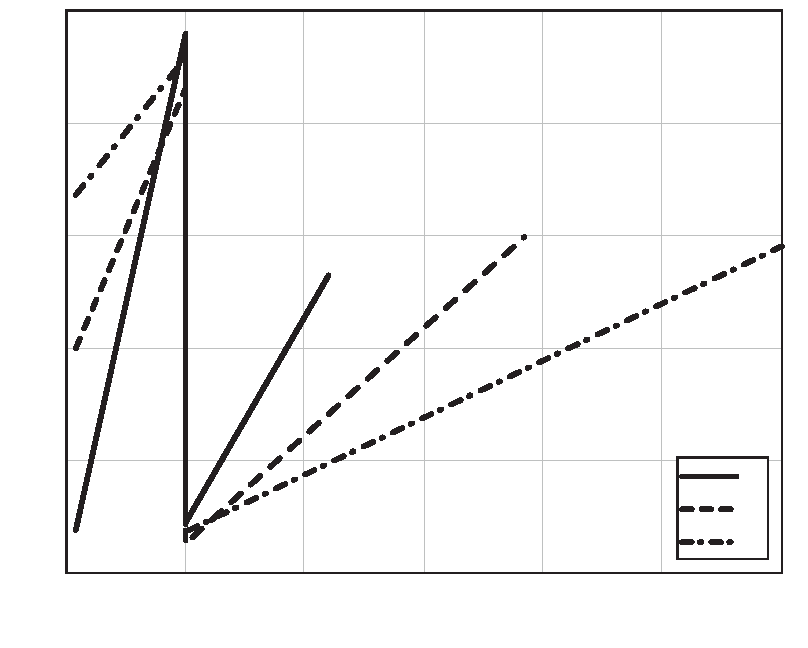
\includegraphics[width=\unitlength]{sigma_z_bf33_comp_3thickness.pdf}}%
        \put(0.06979721,0.0514458){\color[named]{black}\makebox(0,0)[lb]{\smash{$ - $0,5}}}%
        \put(0.22931495,0.05144579){\color[named]{black}\makebox(0,0)[lb]{\smash{0}}}%
        \put(0.36482755,0.05144579){\color[named]{black}\makebox(0,0)[lb]{\smash{0,5}}}%
        \put(0.52558421,0.05144579){\color[named]{black}\makebox(0,0)[lb]{\smash{1}}}%
        \put(0.6610968,0.05144579){\color[named]{black}\makebox(0,0)[lb]{\smash{1,5}}}%
        \put(0.81984013,0.05144579){\color[named]{black}\makebox(0,0)[lb]{\smash{2}}}%
        \put(0.95721119,0.05144579){\color[named]{black}\makebox(0,0)[lb]{\smash{2,5}}}%
        \put(0.07249948,0.21591931){\color[named]{black}\makebox(0,0)[rb]{\smash{$ - $1}}}%
        \put(0.06937633,0.35530369){\color[named]{black}\makebox(0,0)[rb]{\smash{0}}}%
        \put(0.07249948,0.49468808){\color[named]{black}\makebox(0,0)[rb]{\smash{1}}}%
        \put(0.06958807,0.63407247){\color[named]{black}\makebox(0,0)[rb]{\smash{2}}}%
        \put(0.07108789,0.77345685){\color[named]{black}\makebox(0,0)[rb]{\smash{3}}}%
        \put(0.92437842,0.20017409){\color[named]{black}\makebox(0,0)[lb]{\smash{\textsl{1}}}}%
        \put(0.92437842,0.15959775){\color[named]{black}\makebox(0,0)[lb]{\smash{\textsl{2}}}}%
        \put(0.92437842,0.11886654){\color[named]{black}\makebox(0,0)[lb]{\smash{\textsl{3}}}}%
        \put(0.52553513,0.00601688){\color[named]{black}\makebox(0,0)[b]{\smash{$ z $, мм}}}%
        \put(0.025091,0.43777503){\color[named]{black}\rotatebox{90}{\makebox(0,0)[b]{\smash{$\sigma_x^T$, МПа}}}}%
        \put(0.06958807,0.0837627){\color[named]{black}\makebox(0,0)[rb]{\smash{$ - $2}}}%
      \end{picture}%
    \endgroup%

    \caption{Графики расчётного распределения остаточных напряжений по~толщине сборки при $T_w =$~20~{\textdegree}C ($T_b =$~270~{\textdegree}C), для случая сборки кремния со~стеклом Borofloat 33 нескольких толщин:}
    \label{fig:sigma_z_bf33_comp_3thickness}
    \textsl{1} "--- толщина стекла 0,6 мм; \textsl{2} "--- толщина стекла 1,4 мм; \textsl{3} "--- толщина стекла~2,5~мм%
\end{figure}

\begin{figure}[!ht]
    \centering
    \begingroup%
      \makeatletter%
      \providecommand\color[2][]{%
        \errmessage{(Inkscape) Color is used for the text in Inkscape, but the package 'color.sty' is not loaded}%
        \renewcommand\color[2][]{}%
      }%
      \providecommand\transparent[1]{%
        \errmessage{(Inkscape) Transparency is used (non-zero) for the text in Inkscape, but the package 'transparent.sty' is not loaded}%
        \renewcommand\transparent[1]{}%
      }%
      \providecommand\rotatebox[2]{#2}%
      \ifx\svgwidth\undefined%
        \setlength{\unitlength}{0.6\textwidth}%
        \ifx\svgscale\undefined%
          \relax%
        \else%
          \setlength{\unitlength}{\unitlength * \real{\svgscale}}%
        \fi%
      \else%
        \setlength{\unitlength}{\svgwidth}%
      \fi%
      \global\let\svgwidth\undefined%
      \global\let\svgscale\undefined%
      \makeatother%
      \begin{picture}(1,0.79779126)%
        \put(0,0){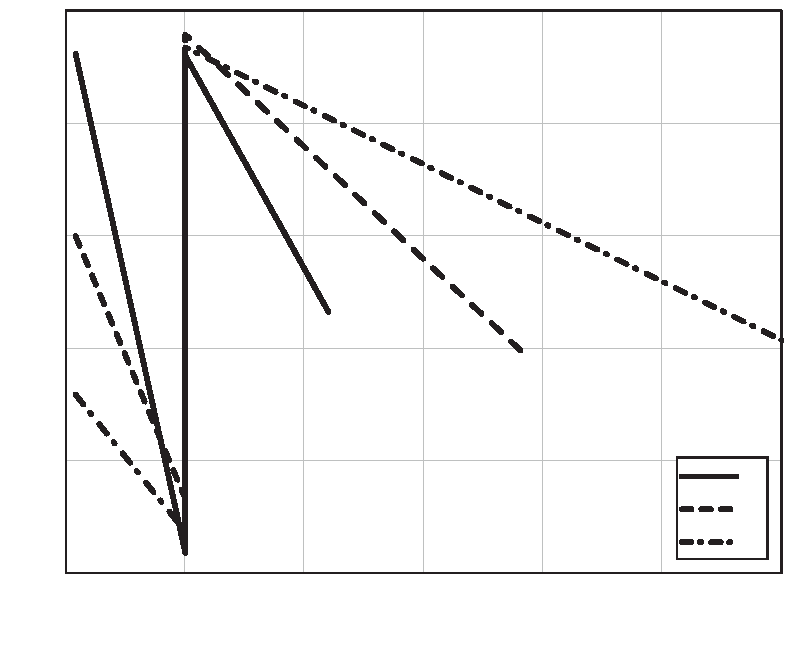
\includegraphics[width=\unitlength]{sigma_z_lk5_comp_3thickness.pdf}}%
        \put(0.06843194,0.21583314){\color[named]{black}\makebox(0,0)[rb]{\smash{$ - $4}}}%
        \put(0.06867897,0.35521754){\color[named]{black}\makebox(0,0)[rb]{\smash{$ - $2}}}%
        \put(0.06846723,0.49460195){\color[named]{black}\makebox(0,0)[rb]{\smash{0}}}%
        \put(0.06867897,0.63398635){\color[named]{black}\makebox(0,0)[rb]{\smash{2}}}%
        \put(0.06843194,0.77337075){\color[named]{black}\makebox(0,0)[rb]{\smash{4}}}%
        \put(0.06979721,0.0514458){\color[named]{black}\makebox(0,0)[lb]{\smash{$ - $0,5}}}%
        \put(0.22931493,0.0514458){\color[named]{black}\makebox(0,0)[lb]{\smash{0}}}%
        \put(0.36482762,0.0514458){\color[named]{black}\makebox(0,0)[lb]{\smash{0,5}}}%
        \put(0.52558418,0.0514458){\color[named]{black}\makebox(0,0)[lb]{\smash{1}}}%
        \put(0.66109679,0.0514458){\color[named]{black}\makebox(0,0)[lb]{\smash{1,5}}}%
        \put(0.81984014,0.0514458){\color[named]{black}\makebox(0,0)[lb]{\smash{2}}}%
        \put(0.95721122,0.0514458){\color[named]{black}\makebox(0,0)[lb]{\smash{2,5}}}%
        \put(0.92437852,0.2001741){\color[named]{black}\makebox(0,0)[lb]{\smash{\textsl{1}}}}%
        \put(0.92437852,0.15959783){\color[named]{black}\makebox(0,0)[lb]{\smash{\textsl{2}}}}%
        \put(0.92437852,0.11886654){\color[named]{black}\makebox(0,0)[lb]{\smash{\textsl{3}}}}%
        \put(0.52525113,0.00601687){\color[named]{black}\makebox(0,0)[b]{\smash{$z$, мм}}}%
        \put(0,0.40712119){\color[named]{black}\rotatebox{90}{\makebox(0,0)[b]{\smash{$\sigma_x^T$, МПа}}}}%
        \put(0.0685731,0.07622534){\color[named]{black}\makebox(0,0)[rb]{\smash{$-$6}}}%
      \end{picture}%
    \endgroup%

    \caption{Графики расчётного распределения остаточных напряжений по~толщине сборки при $T_w =$~20~{\textdegree}C ($T_b =$~270~{\textdegree}C), для случая сборки кремния со стеклом ЛК5 нескольких толщин:}
    \label{fig:sigma_z_lk5_comp_3thickness}
    \textsl{1} "--- толщина стекла 0,6 мм; \textsl{2} "--- толщина стекла 1,4 мм; \textsl{3} "--- толщина стекла~2,5~мм%
\end{figure}

Если проводить расчёт с допущением об отсутствии зависимости жёсткостей стекла и кремния  от температуры, то из Рисунков~\ref{fig:glass_stress_multilayer_ot_h_tw},~\ref{fig:glass_stress_multilayer_ot_h_tb},~\ref{fig:sigma_ot_h_rus} и~\ref{fig:sigma_ot_h85_rus} видно, что для каждой из рассматриваемых марок стекла есть такое отношение толщины стекла к толщине кремния, при котором остаточные напряжения на~несоединённой поверхности кремния будут равны нулю во всём рабочем диапазоне температур.

Это отношение зависит от жёсткости стекла и его расчётное значение приведено в Таблице~\ref{tab_h0_stekla}.

Подбирать толщину стекла с целью получения минимальных напряжений
на~некоторой глубине от~свободной поверхности кремния возможно среди
тех толщин стекла, при которых напряжения в~кремнии меняют знак
по~толщине пластины. Это приводит к следующим расчётным ограничениям
на~глубину возможного зануления напряжений:
\begin{itemize}
    \item не превышает трети от толщины пластины кремния;
    \item уменьшается с увеличением толщины стекла.
\end{itemize}%
\begingroup%
В случае
несплошного контакта соединяемых
кремния и стекла, моделирование конечными элементами показало, что
искомая толщина будет меньше пропорционально уменьшению площади
границы соединения кремния со~стеклом.\russianpar
\endgroup

\begin{figure}[!ht]%
    \centering%
    \subcaptionbox{\label{fig:glass_stress_multilayer_ot_h_tw}}
    {%
        \ifdefmacro{\tikzsetnextfilename}{\tikzsetnextfilename{glass_stress_multilayer_ot_h_tw}}{}%
        % Created by tikzDevice version 0.10.1 on 2016-10-01 21:04:21
% !TEX encoding = UTF-8 Unicode
\begin{tikzpicture}[x=1pt,y=1pt]
\definecolor{fillColor}{RGB}{255,255,255}
\path[use as bounding box,fill=fillColor] (0,0) rectangle (241.85,217.66);
\begin{scope}
\path[clip] (  0.00,  0.00) rectangle (241.85,217.66);
\definecolor{drawColor}{RGB}{255,255,255}

\path[draw=drawColor,line width= 0.6pt,line join=round,line cap=round,fill=fillColor] ( -0.00,  0.00) rectangle (241.85,217.66);
\end{scope}
\begin{scope}
\path[clip] ( 45.96, 34.42) rectangle (237.63,217.66);
\definecolor{fillColor}{RGB}{255,255,255}

\path[fill=fillColor] ( 45.96, 34.42) rectangle (237.63,217.66);
\definecolor{drawColor}{gray}{0.98}

\path[draw=drawColor,line width= 0.6pt,line join=round] ( 45.96, 64.36) --
	(237.63, 64.36);

\path[draw=drawColor,line width= 0.6pt,line join=round] ( 45.96, 96.62) --
	(237.63, 96.62);

\path[draw=drawColor,line width= 0.6pt,line join=round] ( 45.96,128.88) --
	(237.63,128.88);

\path[draw=drawColor,line width= 0.6pt,line join=round] ( 45.96,161.14) --
	(237.63,161.14);

\path[draw=drawColor,line width= 0.6pt,line join=round] ( 45.96,193.40) --
	(237.63,193.40);

\path[draw=drawColor,line width= 0.6pt,line join=round] ( 72.10, 34.42) --
	( 72.10,217.66);

\path[draw=drawColor,line width= 0.6pt,line join=round] (106.95, 34.42) --
	(106.95,217.66);

\path[draw=drawColor,line width= 0.6pt,line join=round] (141.80, 34.42) --
	(141.80,217.66);

\path[draw=drawColor,line width= 0.6pt,line join=round] (176.65, 34.42) --
	(176.65,217.66);

\path[draw=drawColor,line width= 0.6pt,line join=round] (211.50, 34.42) --
	(211.50,217.66);
\definecolor{drawColor}{gray}{0.80}

\path[draw=drawColor,line width= 0.3pt,line join=round] ( 45.96, 48.23) --
	(237.63, 48.23);

\path[draw=drawColor,line width= 0.3pt,line join=round] ( 45.96, 80.49) --
	(237.63, 80.49);

\path[draw=drawColor,line width= 0.3pt,line join=round] ( 45.96,112.75) --
	(237.63,112.75);

\path[draw=drawColor,line width= 0.3pt,line join=round] ( 45.96,145.01) --
	(237.63,145.01);

\path[draw=drawColor,line width= 0.3pt,line join=round] ( 45.96,177.27) --
	(237.63,177.27);

\path[draw=drawColor,line width= 0.3pt,line join=round] ( 45.96,209.53) --
	(237.63,209.53);

\path[draw=drawColor,line width= 0.3pt,line join=round] ( 54.67, 34.42) --
	( 54.67,217.66);

\path[draw=drawColor,line width= 0.3pt,line join=round] ( 89.52, 34.42) --
	( 89.52,217.66);

\path[draw=drawColor,line width= 0.3pt,line join=round] (124.37, 34.42) --
	(124.37,217.66);

\path[draw=drawColor,line width= 0.3pt,line join=round] (159.22, 34.42) --
	(159.22,217.66);

\path[draw=drawColor,line width= 0.3pt,line join=round] (194.07, 34.42) --
	(194.07,217.66);

\path[draw=drawColor,line width= 0.3pt,line join=round] (228.92, 34.42) --
	(228.92,217.66);
\definecolor{drawColor}{RGB}{0,0,0}

\path[draw=drawColor,line width= 1.4pt,line join=round] ( 54.67,145.01) --
	( 55.25,145.54) --
	( 55.83,146.06) --
	( 56.42,146.59) --
	( 57.00,147.10) --
	( 57.58,147.61) --
	( 58.16,148.11) --
	( 58.74,148.60) --
	( 59.32,149.08) --
	( 59.90,149.54) --
	( 60.48,149.99) --
	( 61.06,150.43) --
	( 61.64,150.85) --
	( 62.22,151.26) --
	( 62.80,151.66) --
	( 63.39,152.03) --
	( 63.97,152.39) --
	( 64.55,152.74) --
	( 65.13,153.07) --
	( 65.71,153.38) --
	( 66.29,153.67) --
	( 66.87,153.95) --
	( 67.45,154.22) --
	( 68.03,154.47) --
	( 68.61,154.70) --
	( 69.19,154.92) --
	( 69.77,155.12) --
	( 70.36,155.31) --
	( 70.94,155.49) --
	( 71.52,155.65) --
	( 72.10,155.80) --
	( 72.68,155.94) --
	( 73.26,156.06) --
	( 73.84,156.18) --
	( 74.42,156.28) --
	( 75.00,156.37) --
	( 75.58,156.46) --
	( 76.16,156.53) --
	( 76.74,156.59) --
	( 77.33,156.64) --
	( 77.91,156.69) --
	( 78.49,156.73) --
	( 79.07,156.76) --
	( 79.65,156.78) --
	( 80.23,156.79) --
	( 80.81,156.80) --
	( 81.39,156.80) --
	( 81.97,156.79) --
	( 82.55,156.78) --
	( 83.13,156.77) --
	( 83.71,156.74) --
	( 84.30,156.72) --
	( 84.88,156.69) --
	( 85.46,156.65) --
	( 86.04,156.61) --
	( 86.62,156.56) --
	( 87.20,156.52) --
	( 87.78,156.46) --
	( 88.36,156.41) --
	( 88.94,156.35) --
	( 89.52,156.29) --
	( 90.10,156.22) --
	( 90.68,156.16) --
	( 91.27,156.09) --
	( 91.85,156.01) --
	( 92.43,155.94) --
	( 93.01,155.86) --
	( 93.59,155.79) --
	( 94.17,155.70) --
	( 94.75,155.62) --
	( 95.33,155.54) --
	( 95.91,155.45) --
	( 96.49,155.37) --
	( 97.07,155.28) --
	( 97.65,155.19) --
	( 98.24,155.10) --
	( 98.82,155.01) --
	( 99.40,154.91) --
	( 99.98,154.82) --
	(100.56,154.73) --
	(101.14,154.63) --
	(101.72,154.54) --
	(102.30,154.44) --
	(102.88,154.34) --
	(103.46,154.25) --
	(104.04,154.15) --
	(104.62,154.05) --
	(105.20,153.95) --
	(105.79,153.85) --
	(106.37,153.75) --
	(106.95,153.65) --
	(107.53,153.55) --
	(108.11,153.45) --
	(108.69,153.35) --
	(109.27,153.25) --
	(109.85,153.15) --
	(110.43,153.05) --
	(111.01,152.95) --
	(111.59,152.84) --
	(112.17,152.74) --
	(112.76,152.64) --
	(113.34,152.54) --
	(113.92,152.44) --
	(114.50,152.34) --
	(115.08,152.24) --
	(115.66,152.14) --
	(116.24,152.04) --
	(116.82,151.94) --
	(117.40,151.84) --
	(117.98,151.74) --
	(118.56,151.64) --
	(119.14,151.54) --
	(119.73,151.44) --
	(120.31,151.34) --
	(120.89,151.24) --
	(121.47,151.14) --
	(122.05,151.04) --
	(122.63,150.95) --
	(123.21,150.85) --
	(123.79,150.75) --
	(124.37,150.65) --
	(124.95,150.56) --
	(125.53,150.46) --
	(126.11,150.36) --
	(126.70,150.27) --
	(127.28,150.17) --
	(127.86,150.07) --
	(128.44,149.98) --
	(129.02,149.88) --
	(129.60,149.79) --
	(130.18,149.70) --
	(130.76,149.60) --
	(131.34,149.51) --
	(131.92,149.41) --
	(132.50,149.32) --
	(133.08,149.23) --
	(133.67,149.14) --
	(134.25,149.04) --
	(134.83,148.95) --
	(135.41,148.86) --
	(135.99,148.77) --
	(136.57,148.68) --
	(137.15,148.59) --
	(137.73,148.50) --
	(138.31,148.41) --
	(138.89,148.32) --
	(139.47,148.23) --
	(140.05,148.14) --
	(140.64,148.06) --
	(141.22,147.97) --
	(141.80,147.88) --
	(142.38,147.79) --
	(142.96,147.71) --
	(143.54,147.62) --
	(144.12,147.53) --
	(144.70,147.45) --
	(145.28,147.36) --
	(145.86,147.28) --
	(146.44,147.19) --
	(147.02,147.11) --
	(147.61,147.03) --
	(148.19,146.94) --
	(148.77,146.86) --
	(149.35,146.78) --
	(149.93,146.69) --
	(150.51,146.61) --
	(151.09,146.53) --
	(151.67,146.45) --
	(152.25,146.37) --
	(152.83,146.29) --
	(153.41,146.21) --
	(153.99,146.13) --
	(154.57,146.05) --
	(155.16,145.97) --
	(155.74,145.89) --
	(156.32,145.81) --
	(156.90,145.73) --
	(157.48,145.65) --
	(158.06,145.57) --
	(158.64,145.50) --
	(159.22,145.42) --
	(159.80,145.34) --
	(160.38,145.26) --
	(160.96,145.19) --
	(161.54,145.11) --
	(162.13,145.04) --
	(162.71,144.96) --
	(163.29,144.89) --
	(163.87,144.81) --
	(164.45,144.74) --
	(165.03,144.66) --
	(165.61,144.59) --
	(166.19,144.51) --
	(166.77,144.44) --
	(167.35,144.37) --
	(167.93,144.30) --
	(168.51,144.22) --
	(169.10,144.15) --
	(169.68,144.08) --
	(170.26,144.01) --
	(170.84,143.94) --
	(171.42,143.87) --
	(172.00,143.79) --
	(172.58,143.72) --
	(173.16,143.65) --
	(173.74,143.58) --
	(174.32,143.51) --
	(174.90,143.45) --
	(175.48,143.38) --
	(176.07,143.31) --
	(176.65,143.24) --
	(177.23,143.17) --
	(177.81,143.10) --
	(178.39,143.04) --
	(178.97,142.97) --
	(179.55,142.90) --
	(180.13,142.83) --
	(180.71,142.77) --
	(181.29,142.70) --
	(181.87,142.63) --
	(182.45,142.57) --
	(183.04,142.50) --
	(183.62,142.44) --
	(184.20,142.37) --
	(184.78,142.31) --
	(185.36,142.24) --
	(185.94,142.18) --
	(186.52,142.11) --
	(187.10,142.05) --
	(187.68,141.99) --
	(188.26,141.92) --
	(188.84,141.86) --
	(189.42,141.80) --
	(190.01,141.73) --
	(190.59,141.67) --
	(191.17,141.61) --
	(191.75,141.55) --
	(192.33,141.49) --
	(192.91,141.42) --
	(193.49,141.36) --
	(194.07,141.30) --
	(194.65,141.24) --
	(195.23,141.18) --
	(195.81,141.12) --
	(196.39,141.06) --
	(196.98,141.00) --
	(197.56,140.94) --
	(198.14,140.88) --
	(198.72,140.82) --
	(199.30,140.76) --
	(199.88,140.70) --
	(200.46,140.64) --
	(201.04,140.59) --
	(201.62,140.53) --
	(202.20,140.47) --
	(202.78,140.41) --
	(203.36,140.35) --
	(203.94,140.30) --
	(204.53,140.24) --
	(205.11,140.18) --
	(205.69,140.12) --
	(206.27,140.07) --
	(206.85,140.01) --
	(207.43,139.95) --
	(208.01,139.90) --
	(208.59,139.84) --
	(209.17,139.79) --
	(209.75,139.73) --
	(210.33,139.68) --
	(210.91,139.62) --
	(211.50,139.57) --
	(212.08,139.51) --
	(212.66,139.46) --
	(213.24,139.40) --
	(213.82,139.35) --
	(214.40,139.29) --
	(214.98,139.24) --
	(215.56,139.19) --
	(216.14,139.13) --
	(216.72,139.08) --
	(217.30,139.03) --
	(217.88,138.97) --
	(218.47,138.92) --
	(219.05,138.87) --
	(219.63,138.82) --
	(220.21,138.76) --
	(220.79,138.71) --
	(221.37,138.66) --
	(221.95,138.61) --
	(222.53,138.56) --
	(223.11,138.51) --
	(223.69,138.45) --
	(224.27,138.40) --
	(224.85,138.35) --
	(225.44,138.30) --
	(226.02,138.25) --
	(226.60,138.20) --
	(227.18,138.15) --
	(227.76,138.10) --
	(228.34,138.05) --
	(228.92,138.00);

\path[draw=drawColor,line width= 1.4pt,dash pattern=on 7pt off 3pt ,line join=round] ( 54.67,145.01) --
	( 55.25,147.96) --
	( 55.83,150.88) --
	( 56.42,153.79) --
	( 57.00,156.65) --
	( 57.58,159.47) --
	( 58.16,162.23) --
	( 58.74,164.94) --
	( 59.32,167.57) --
	( 59.90,170.14) --
	( 60.48,172.63) --
	( 61.06,175.03) --
	( 61.64,177.36) --
	( 62.22,179.60) --
	( 62.80,181.74) --
	( 63.39,183.80) --
	( 63.97,185.77) --
	( 64.55,187.65) --
	( 65.13,189.43) --
	( 65.71,191.13) --
	( 66.29,192.73) --
	( 66.87,194.25) --
	( 67.45,195.67) --
	( 68.03,197.02) --
	( 68.61,198.27) --
	( 69.19,199.45) --
	( 69.77,200.54) --
	( 70.36,201.56) --
	( 70.94,202.50) --
	( 71.52,203.37) --
	( 72.10,204.17) --
	( 72.68,204.90) --
	( 73.26,205.56) --
	( 73.84,206.17) --
	( 74.42,206.71) --
	( 75.00,207.19) --
	( 75.58,207.61) --
	( 76.16,207.98) --
	( 76.74,208.31) --
	( 77.33,208.58) --
	( 77.91,208.80) --
	( 78.49,208.98) --
	( 79.07,209.12) --
	( 79.65,209.21) --
	( 80.23,209.27) --
	( 80.81,209.29) --
	( 81.39,209.28) --
	( 81.97,209.23) --
	( 82.55,209.15) --
	( 83.13,209.04) --
	( 83.71,208.91) --
	( 84.30,208.74) --
	( 84.88,208.55) --
	( 85.46,208.34) --
	( 86.04,208.10) --
	( 86.62,207.84) --
	( 87.20,207.56) --
	( 87.78,207.26) --
	( 88.36,206.95) --
	( 88.94,206.61) --
	( 89.52,206.26) --
	( 90.10,205.89) --
	( 90.68,205.51) --
	( 91.27,205.12) --
	( 91.85,204.71) --
	( 92.43,204.29) --
	( 93.01,203.86) --
	( 93.59,203.42) --
	( 94.17,202.97) --
	( 94.75,202.51) --
	( 95.33,202.05) --
	( 95.91,201.57) --
	( 96.49,201.09) --
	( 97.07,200.59) --
	( 97.65,200.10) --
	( 98.24,199.59) --
	( 98.82,199.08) --
	( 99.40,198.57) --
	( 99.98,198.05) --
	(100.56,197.53) --
	(101.14,197.00) --
	(101.72,196.47) --
	(102.30,195.93) --
	(102.88,195.39) --
	(103.46,194.85) --
	(104.04,194.31) --
	(104.62,193.76) --
	(105.20,193.21) --
	(105.79,192.66) --
	(106.37,192.11) --
	(106.95,191.56) --
	(107.53,191.01) --
	(108.11,190.45) --
	(108.69,189.89) --
	(109.27,189.34) --
	(109.85,188.78) --
	(110.43,188.22) --
	(111.01,187.67) --
	(111.59,187.11) --
	(112.17,186.55) --
	(112.76,185.99) --
	(113.34,185.44) --
	(113.92,184.88) --
	(114.50,184.32) --
	(115.08,183.77) --
	(115.66,183.21) --
	(116.24,182.66) --
	(116.82,182.10) --
	(117.40,181.55) --
	(117.98,181.00) --
	(118.56,180.45) --
	(119.14,179.90) --
	(119.73,179.35) --
	(120.31,178.81) --
	(120.89,178.26) --
	(121.47,177.72) --
	(122.05,177.18) --
	(122.63,176.64) --
	(123.21,176.10) --
	(123.79,175.56) --
	(124.37,175.02) --
	(124.95,174.49) --
	(125.53,173.95) --
	(126.11,173.42) --
	(126.70,172.89) --
	(127.28,172.37) --
	(127.86,171.84) --
	(128.44,171.32) --
	(129.02,170.79) --
	(129.60,170.27) --
	(130.18,169.75) --
	(130.76,169.24) --
	(131.34,168.72) --
	(131.92,168.21) --
	(132.50,167.70) --
	(133.08,167.19) --
	(133.67,166.68) --
	(134.25,166.17) --
	(134.83,165.67) --
	(135.41,165.17) --
	(135.99,164.67) --
	(136.57,164.17) --
	(137.15,163.67) --
	(137.73,163.18) --
	(138.31,162.69) --
	(138.89,162.20) --
	(139.47,161.71) --
	(140.05,161.22) --
	(140.64,160.74) --
	(141.22,160.26) --
	(141.80,159.78) --
	(142.38,159.30) --
	(142.96,158.82) --
	(143.54,158.35) --
	(144.12,157.87) --
	(144.70,157.40) --
	(145.28,156.93) --
	(145.86,156.47) --
	(146.44,156.00) --
	(147.02,155.54) --
	(147.61,155.08) --
	(148.19,154.62) --
	(148.77,154.16) --
	(149.35,153.71) --
	(149.93,153.25) --
	(150.51,152.80) --
	(151.09,152.35) --
	(151.67,151.90) --
	(152.25,151.46) --
	(152.83,151.01) --
	(153.41,150.57) --
	(153.99,150.13) --
	(154.57,149.69) --
	(155.16,149.25) --
	(155.74,148.82) --
	(156.32,148.39) --
	(156.90,147.95) --
	(157.48,147.52) --
	(158.06,147.10) --
	(158.64,146.67) --
	(159.22,146.25) --
	(159.80,145.82) --
	(160.38,145.40) --
	(160.96,144.98) --
	(161.54,144.57) --
	(162.13,144.15) --
	(162.71,143.74) --
	(163.29,143.32) --
	(163.87,142.91) --
	(164.45,142.50) --
	(165.03,142.10) --
	(165.61,141.69) --
	(166.19,141.29) --
	(166.77,140.88) --
	(167.35,140.48) --
	(167.93,140.08) --
	(168.51,139.69) --
	(169.10,139.29) --
	(169.68,138.90) --
	(170.26,138.50) --
	(170.84,138.11) --
	(171.42,137.72) --
	(172.00,137.33) --
	(172.58,136.95) --
	(173.16,136.56) --
	(173.74,136.18) --
	(174.32,135.80) --
	(174.90,135.42) --
	(175.48,135.04) --
	(176.07,134.66) --
	(176.65,134.29) --
	(177.23,133.91) --
	(177.81,133.54) --
	(178.39,133.17) --
	(178.97,132.80) --
	(179.55,132.43) --
	(180.13,132.06) --
	(180.71,131.70) --
	(181.29,131.33) --
	(181.87,130.97) --
	(182.45,130.61) --
	(183.04,130.25) --
	(183.62,129.89) --
	(184.20,129.53) --
	(184.78,129.17) --
	(185.36,128.82) --
	(185.94,128.47) --
	(186.52,128.11) --
	(187.10,127.76) --
	(187.68,127.41) --
	(188.26,127.07) --
	(188.84,126.72) --
	(189.42,126.38) --
	(190.01,126.03) --
	(190.59,125.69) --
	(191.17,125.35) --
	(191.75,125.01) --
	(192.33,124.67) --
	(192.91,124.33) --
	(193.49,123.99) --
	(194.07,123.66) --
	(194.65,123.32) --
	(195.23,122.99) --
	(195.81,122.66) --
	(196.39,122.33) --
	(196.98,122.00) --
	(197.56,121.67) --
	(198.14,121.35) --
	(198.72,121.02) --
	(199.30,120.70) --
	(199.88,120.37) --
	(200.46,120.05) --
	(201.04,119.73) --
	(201.62,119.41) --
	(202.20,119.09) --
	(202.78,118.78) --
	(203.36,118.46) --
	(203.94,118.15) --
	(204.53,117.83) --
	(205.11,117.52) --
	(205.69,117.21) --
	(206.27,116.90) --
	(206.85,116.59) --
	(207.43,116.28) --
	(208.01,115.97) --
	(208.59,115.67) --
	(209.17,115.36) --
	(209.75,115.06) --
	(210.33,114.75) --
	(210.91,114.45) --
	(211.50,114.15) --
	(212.08,113.85) --
	(212.66,113.55) --
	(213.24,113.25) --
	(213.82,112.96) --
	(214.40,112.66) --
	(214.98,112.37) --
	(215.56,112.07) --
	(216.14,111.78) --
	(216.72,111.49) --
	(217.30,111.20) --
	(217.88,110.91) --
	(218.47,110.62) --
	(219.05,110.33) --
	(219.63,110.04) --
	(220.21,109.76) --
	(220.79,109.47) --
	(221.37,109.19) --
	(221.95,108.91) --
	(222.53,108.62) --
	(223.11,108.34) --
	(223.69,108.06) --
	(224.27,107.78) --
	(224.85,107.50) --
	(225.44,107.23) --
	(226.02,106.95) --
	(226.60,106.67) --
	(227.18,106.40) --
	(227.76,106.13) --
	(228.34,105.85) --
	(228.92,105.58);
\definecolor{drawColor}{RGB}{149,149,149}

\path[draw=drawColor,line width= 1.4pt,line join=round] ( 54.67,145.01) --
	( 55.25,144.02) --
	( 55.83,143.04) --
	( 56.42,142.07) --
	( 57.00,141.10) --
	( 57.58,140.15) --
	( 58.16,139.22) --
	( 58.74,138.31) --
	( 59.32,137.41) --
	( 59.90,136.55) --
	( 60.48,135.70) --
	( 61.06,134.88) --
	( 61.64,134.09) --
	( 62.22,133.33) --
	( 62.80,132.60) --
	( 63.39,131.89) --
	( 63.97,131.22) --
	( 64.55,130.57) --
	( 65.13,129.96) --
	( 65.71,129.38) --
	( 66.29,128.83) --
	( 66.87,128.30) --
	( 67.45,127.81) --
	( 68.03,127.35) --
	( 68.61,126.91) --
	( 69.19,126.50) --
	( 69.77,126.12) --
	( 70.36,125.77) --
	( 70.94,125.44) --
	( 71.52,125.13) --
	( 72.10,124.85) --
	( 72.68,124.59) --
	( 73.26,124.36) --
	( 73.84,124.15) --
	( 74.42,123.95) --
	( 75.00,123.78) --
	( 75.58,123.63) --
	( 76.16,123.49) --
	( 76.74,123.38) --
	( 77.33,123.28) --
	( 77.91,123.19) --
	( 78.49,123.12) --
	( 79.07,123.07) --
	( 79.65,123.03) --
	( 80.23,123.00) --
	( 80.81,122.99) --
	( 81.39,122.99) --
	( 81.97,123.00) --
	( 82.55,123.02) --
	( 83.13,123.05) --
	( 83.71,123.09) --
	( 84.30,123.14) --
	( 84.88,123.20) --
	( 85.46,123.27) --
	( 86.04,123.34) --
	( 86.62,123.43) --
	( 87.20,123.52) --
	( 87.78,123.61) --
	( 88.36,123.72) --
	( 88.94,123.83) --
	( 89.52,123.94) --
	( 90.10,124.06) --
	( 90.68,124.19) --
	( 91.27,124.32) --
	( 91.85,124.45) --
	( 92.43,124.59) --
	( 93.01,124.73) --
	( 93.59,124.88) --
	( 94.17,125.03) --
	( 94.75,125.19) --
	( 95.33,125.34) --
	( 95.91,125.50) --
	( 96.49,125.66) --
	( 97.07,125.83) --
	( 97.65,125.99) --
	( 98.24,126.16) --
	( 98.82,126.33) --
	( 99.40,126.51) --
	( 99.98,126.68) --
	(100.56,126.86) --
	(101.14,127.04) --
	(101.72,127.21) --
	(102.30,127.39) --
	(102.88,127.58) --
	(103.46,127.76) --
	(104.04,127.94) --
	(104.62,128.13) --
	(105.20,128.31) --
	(105.79,128.50) --
	(106.37,128.68) --
	(106.95,128.87) --
	(107.53,129.06) --
	(108.11,129.24) --
	(108.69,129.43) --
	(109.27,129.62) --
	(109.85,129.81) --
	(110.43,130.00) --
	(111.01,130.18) --
	(111.59,130.37) --
	(112.17,130.56) --
	(112.76,130.75) --
	(113.34,130.94) --
	(113.92,131.13) --
	(114.50,131.32) --
	(115.08,131.50) --
	(115.66,131.69) --
	(116.24,131.88) --
	(116.82,132.07) --
	(117.40,132.25) --
	(117.98,132.44) --
	(118.56,132.63) --
	(119.14,132.81) --
	(119.73,133.00) --
	(120.31,133.18) --
	(120.89,133.37) --
	(121.47,133.55) --
	(122.05,133.74) --
	(122.63,133.92) --
	(123.21,134.10) --
	(123.79,134.29) --
	(124.37,134.47) --
	(124.95,134.65) --
	(125.53,134.83) --
	(126.11,135.01) --
	(126.70,135.19) --
	(127.28,135.37) --
	(127.86,135.55) --
	(128.44,135.73) --
	(129.02,135.90) --
	(129.60,136.08) --
	(130.18,136.26) --
	(130.76,136.43) --
	(131.34,136.61) --
	(131.92,136.78) --
	(132.50,136.95) --
	(133.08,137.13) --
	(133.67,137.30) --
	(134.25,137.47) --
	(134.83,137.64) --
	(135.41,137.81) --
	(135.99,137.98) --
	(136.57,138.15) --
	(137.15,138.32) --
	(137.73,138.49) --
	(138.31,138.66) --
	(138.89,138.82) --
	(139.47,138.99) --
	(140.05,139.15) --
	(140.64,139.32) --
	(141.22,139.48) --
	(141.80,139.65) --
	(142.38,139.81) --
	(142.96,139.97) --
	(143.54,140.13) --
	(144.12,140.29) --
	(144.70,140.45) --
	(145.28,140.61) --
	(145.86,140.77) --
	(146.44,140.93) --
	(147.02,141.08) --
	(147.61,141.24) --
	(148.19,141.40) --
	(148.77,141.55) --
	(149.35,141.71) --
	(149.93,141.86) --
	(150.51,142.02) --
	(151.09,142.17) --
	(151.67,142.32) --
	(152.25,142.47) --
	(152.83,142.62) --
	(153.41,142.77) --
	(153.99,142.92) --
	(154.57,143.07) --
	(155.16,143.22) --
	(155.74,143.37) --
	(156.32,143.52) --
	(156.90,143.66) --
	(157.48,143.81) --
	(158.06,143.96) --
	(158.64,144.10) --
	(159.22,144.24) --
	(159.80,144.39) --
	(160.38,144.53) --
	(160.96,144.67) --
	(161.54,144.82) --
	(162.13,144.96) --
	(162.71,145.10) --
	(163.29,145.24) --
	(163.87,145.38) --
	(164.45,145.52) --
	(165.03,145.66) --
	(165.61,145.79) --
	(166.19,145.93) --
	(166.77,146.07) --
	(167.35,146.21) --
	(167.93,146.34) --
	(168.51,146.48) --
	(169.10,146.61) --
	(169.68,146.75) --
	(170.26,146.88) --
	(170.84,147.01) --
	(171.42,147.14) --
	(172.00,147.28) --
	(172.58,147.41) --
	(173.16,147.54) --
	(173.74,147.67) --
	(174.32,147.80) --
	(174.90,147.93) --
	(175.48,148.06) --
	(176.07,148.19) --
	(176.65,148.31) --
	(177.23,148.44) --
	(177.81,148.57) --
	(178.39,148.70) --
	(178.97,148.82) --
	(179.55,148.95) --
	(180.13,149.07) --
	(180.71,149.20) --
	(181.29,149.32) --
	(181.87,149.44) --
	(182.45,149.57) --
	(183.04,149.69) --
	(183.62,149.81) --
	(184.20,149.93) --
	(184.78,150.06) --
	(185.36,150.18) --
	(185.94,150.30) --
	(186.52,150.42) --
	(187.10,150.54) --
	(187.68,150.65) --
	(188.26,150.77) --
	(188.84,150.89) --
	(189.42,151.01) --
	(190.01,151.13) --
	(190.59,151.24) --
	(191.17,151.36) --
	(191.75,151.47) --
	(192.33,151.59) --
	(192.91,151.71) --
	(193.49,151.82) --
	(194.07,151.93) --
	(194.65,152.05) --
	(195.23,152.16) --
	(195.81,152.27) --
	(196.39,152.39) --
	(196.98,152.50) --
	(197.56,152.61) --
	(198.14,152.72) --
	(198.72,152.83) --
	(199.30,152.94) --
	(199.88,153.05) --
	(200.46,153.16) --
	(201.04,153.27) --
	(201.62,153.38) --
	(202.20,153.49) --
	(202.78,153.60) --
	(203.36,153.71) --
	(203.94,153.81) --
	(204.53,153.92) --
	(205.11,154.03) --
	(205.69,154.13) --
	(206.27,154.24) --
	(206.85,154.34) --
	(207.43,154.45) --
	(208.01,154.55) --
	(208.59,154.66) --
	(209.17,154.76) --
	(209.75,154.87) --
	(210.33,154.97) --
	(210.91,155.07) --
	(211.50,155.18) --
	(212.08,155.28) --
	(212.66,155.38) --
	(213.24,155.48) --
	(213.82,155.58) --
	(214.40,155.68) --
	(214.98,155.78) --
	(215.56,155.88) --
	(216.14,155.98) --
	(216.72,156.08) --
	(217.30,156.18) --
	(217.88,156.28) --
	(218.47,156.38) --
	(219.05,156.48) --
	(219.63,156.58) --
	(220.21,156.67) --
	(220.79,156.77) --
	(221.37,156.87) --
	(221.95,156.96) --
	(222.53,157.06) --
	(223.11,157.16) --
	(223.69,157.25) --
	(224.27,157.35) --
	(224.85,157.44) --
	(225.44,157.54) --
	(226.02,157.63) --
	(226.60,157.73) --
	(227.18,157.82) --
	(227.76,157.91) --
	(228.34,158.01) --
	(228.92,158.10);

\path[draw=drawColor,line width= 1.4pt,dash pattern=on 7pt off 3pt ,line join=round] ( 54.67,145.01) --
	( 55.25,145.98) --
	( 55.83,146.95) --
	( 56.42,147.91) --
	( 57.00,148.86) --
	( 57.58,149.79) --
	( 58.16,150.70) --
	( 58.74,151.59) --
	( 59.32,152.47) --
	( 59.90,153.31) --
	( 60.48,154.14) --
	( 61.06,154.93) --
	( 61.64,155.70) --
	( 62.22,156.44) --
	( 62.80,157.15) --
	( 63.39,157.83) --
	( 63.97,158.48) --
	( 64.55,159.10) --
	( 65.13,159.69) --
	( 65.71,160.25) --
	( 66.29,160.78) --
	( 66.87,161.28) --
	( 67.45,161.75) --
	( 68.03,162.19) --
	( 68.61,162.61) --
	( 69.19,163.00) --
	( 69.77,163.36) --
	( 70.36,163.70) --
	( 70.94,164.01) --
	( 71.52,164.30) --
	( 72.10,164.56) --
	( 72.68,164.80) --
	( 73.26,165.02) --
	( 73.84,165.22) --
	( 74.42,165.40) --
	( 75.00,165.56) --
	( 75.58,165.70) --
	( 76.16,165.82) --
	( 76.74,165.92) --
	( 77.33,166.01) --
	( 77.91,166.09) --
	( 78.49,166.15) --
	( 79.07,166.19) --
	( 79.65,166.23) --
	( 80.23,166.24) --
	( 80.81,166.25) --
	( 81.39,166.25) --
	( 81.97,166.23) --
	( 82.55,166.20) --
	( 83.13,166.17) --
	( 83.71,166.12) --
	( 84.30,166.07) --
	( 84.88,166.01) --
	( 85.46,165.94) --
	( 86.04,165.86) --
	( 86.62,165.77) --
	( 87.20,165.68) --
	( 87.78,165.58) --
	( 88.36,165.48) --
	( 88.94,165.37) --
	( 89.52,165.25) --
	( 90.10,165.13) --
	( 90.68,165.00) --
	( 91.27,164.87) --
	( 91.85,164.74) --
	( 92.43,164.60) --
	( 93.01,164.46) --
	( 93.59,164.31) --
	( 94.17,164.16) --
	( 94.75,164.01) --
	( 95.33,163.86) --
	( 95.91,163.70) --
	( 96.49,163.54) --
	( 97.07,163.38) --
	( 97.65,163.21) --
	( 98.24,163.05) --
	( 98.82,162.88) --
	( 99.40,162.71) --
	( 99.98,162.54) --
	(100.56,162.36) --
	(101.14,162.19) --
	(101.72,162.01) --
	(102.30,161.84) --
	(102.88,161.66) --
	(103.46,161.48) --
	(104.04,161.30) --
	(104.62,161.12) --
	(105.20,160.94) --
	(105.79,160.76) --
	(106.37,160.57) --
	(106.95,160.39) --
	(107.53,160.21) --
	(108.11,160.02) --
	(108.69,159.84) --
	(109.27,159.66) --
	(109.85,159.47) --
	(110.43,159.29) --
	(111.01,159.10) --
	(111.59,158.92) --
	(112.17,158.74) --
	(112.76,158.55) --
	(113.34,158.37) --
	(113.92,158.18) --
	(114.50,158.00) --
	(115.08,157.82) --
	(115.66,157.63) --
	(116.24,157.45) --
	(116.82,157.27) --
	(117.40,157.08) --
	(117.98,156.90) --
	(118.56,156.72) --
	(119.14,156.54) --
	(119.73,156.36) --
	(120.31,156.18) --
	(120.89,156.00) --
	(121.47,155.82) --
	(122.05,155.64) --
	(122.63,155.46) --
	(123.21,155.28) --
	(123.79,155.10) --
	(124.37,154.93) --
	(124.95,154.75) --
	(125.53,154.57) --
	(126.11,154.40) --
	(126.70,154.22) --
	(127.28,154.05) --
	(127.86,153.88) --
	(128.44,153.70) --
	(129.02,153.53) --
	(129.60,153.36) --
	(130.18,153.19) --
	(130.76,153.01) --
	(131.34,152.84) --
	(131.92,152.67) --
	(132.50,152.51) --
	(133.08,152.34) --
	(133.67,152.17) --
	(134.25,152.00) --
	(134.83,151.84) --
	(135.41,151.67) --
	(135.99,151.51) --
	(136.57,151.34) --
	(137.15,151.18) --
	(137.73,151.01) --
	(138.31,150.85) --
	(138.89,150.69) --
	(139.47,150.53) --
	(140.05,150.37) --
	(140.64,150.21) --
	(141.22,150.05) --
	(141.80,149.89) --
	(142.38,149.73) --
	(142.96,149.57) --
	(143.54,149.42) --
	(144.12,149.26) --
	(144.70,149.10) --
	(145.28,148.95) --
	(145.86,148.80) --
	(146.44,148.64) --
	(147.02,148.49) --
	(147.61,148.34) --
	(148.19,148.18) --
	(148.77,148.03) --
	(149.35,147.88) --
	(149.93,147.73) --
	(150.51,147.58) --
	(151.09,147.44) --
	(151.67,147.29) --
	(152.25,147.14) --
	(152.83,146.99) --
	(153.41,146.85) --
	(153.99,146.70) --
	(154.57,146.56) --
	(155.16,146.41) --
	(155.74,146.27) --
	(156.32,146.13) --
	(156.90,145.98) --
	(157.48,145.84) --
	(158.06,145.70) --
	(158.64,145.56) --
	(159.22,145.42) --
	(159.80,145.28) --
	(160.38,145.14) --
	(160.96,145.00) --
	(161.54,144.86) --
	(162.13,144.73) --
	(162.71,144.59) --
	(163.29,144.45) --
	(163.87,144.32) --
	(164.45,144.18) --
	(165.03,144.05) --
	(165.61,143.91) --
	(166.19,143.78) --
	(166.77,143.65) --
	(167.35,143.51) --
	(167.93,143.38) --
	(168.51,143.25) --
	(169.10,143.12) --
	(169.68,142.99) --
	(170.26,142.86) --
	(170.84,142.73) --
	(171.42,142.60) --
	(172.00,142.47) --
	(172.58,142.35) --
	(173.16,142.22) --
	(173.74,142.09) --
	(174.32,141.97) --
	(174.90,141.84) --
	(175.48,141.71) --
	(176.07,141.59) --
	(176.65,141.47) --
	(177.23,141.34) --
	(177.81,141.22) --
	(178.39,141.10) --
	(178.97,140.97) --
	(179.55,140.85) --
	(180.13,140.73) --
	(180.71,140.61) --
	(181.29,140.49) --
	(181.87,140.37) --
	(182.45,140.25) --
	(183.04,140.13) --
	(183.62,140.01) --
	(184.20,139.89) --
	(184.78,139.78) --
	(185.36,139.66) --
	(185.94,139.54) --
	(186.52,139.43) --
	(187.10,139.31) --
	(187.68,139.20) --
	(188.26,139.08) --
	(188.84,138.97) --
	(189.42,138.85) --
	(190.01,138.74) --
	(190.59,138.62) --
	(191.17,138.51) --
	(191.75,138.40) --
	(192.33,138.29) --
	(192.91,138.18) --
	(193.49,138.06) --
	(194.07,137.95) --
	(194.65,137.84) --
	(195.23,137.73) --
	(195.81,137.62) --
	(196.39,137.52) --
	(196.98,137.41) --
	(197.56,137.30) --
	(198.14,137.19) --
	(198.72,137.08) --
	(199.30,136.98) --
	(199.88,136.87) --
	(200.46,136.76) --
	(201.04,136.66) --
	(201.62,136.55) --
	(202.20,136.45) --
	(202.78,136.34) --
	(203.36,136.24) --
	(203.94,136.13) --
	(204.53,136.03) --
	(205.11,135.93) --
	(205.69,135.82) --
	(206.27,135.72) --
	(206.85,135.62) --
	(207.43,135.52) --
	(208.01,135.41) --
	(208.59,135.31) --
	(209.17,135.21) --
	(209.75,135.11) --
	(210.33,135.01) --
	(210.91,134.91) --
	(211.50,134.81) --
	(212.08,134.71) --
	(212.66,134.61) --
	(213.24,134.52) --
	(213.82,134.42) --
	(214.40,134.32) --
	(214.98,134.22) --
	(215.56,134.13) --
	(216.14,134.03) --
	(216.72,133.93) --
	(217.30,133.84) --
	(217.88,133.74) --
	(218.47,133.64) --
	(219.05,133.55) --
	(219.63,133.45) --
	(220.21,133.36) --
	(220.79,133.27) --
	(221.37,133.17) --
	(221.95,133.08) --
	(222.53,132.99) --
	(223.11,132.89) --
	(223.69,132.80) --
	(224.27,132.71) --
	(224.85,132.62) --
	(225.44,132.52) --
	(226.02,132.43) --
	(226.60,132.34) --
	(227.18,132.25) --
	(227.76,132.16) --
	(228.34,132.07) --
	(228.92,131.98);
\definecolor{drawColor}{gray}{0.80}

\path[draw=drawColor,line width= 1.4pt,line join=round] ( 54.67,145.01) --
	( 55.25,143.52) --
	( 55.83,142.04) --
	( 56.42,140.57) --
	( 57.00,139.12) --
	( 57.58,137.69) --
	( 58.16,136.29) --
	( 58.74,134.91) --
	( 59.32,133.57) --
	( 59.90,132.26) --
	( 60.48,130.98) --
	( 61.06,129.75) --
	( 61.64,128.56) --
	( 62.22,127.41) --
	( 62.80,126.31) --
	( 63.39,125.24) --
	( 63.97,124.23) --
	( 64.55,123.26) --
	( 65.13,122.34) --
	( 65.71,121.46) --
	( 66.29,120.63) --
	( 66.87,119.84) --
	( 67.45,119.09) --
	( 68.03,118.40) --
	( 68.61,117.74) --
	( 69.19,117.12) --
	( 69.77,116.55) --
	( 70.36,116.01) --
	( 70.94,115.52) --
	( 71.52,115.06) --
	( 72.10,114.64) --
	( 72.68,114.25) --
	( 73.26,113.90) --
	( 73.84,113.57) --
	( 74.42,113.28) --
	( 75.00,113.02) --
	( 75.58,112.79) --
	( 76.16,112.59) --
	( 76.74,112.41) --
	( 77.33,112.26) --
	( 77.91,112.14) --
	( 78.49,112.03) --
	( 79.07,111.95) --
	( 79.65,111.89) --
	( 80.23,111.85) --
	( 80.81,111.83) --
	( 81.39,111.83) --
	( 81.97,111.84) --
	( 82.55,111.87) --
	( 83.13,111.92) --
	( 83.71,111.98) --
	( 84.30,112.06) --
	( 84.88,112.15) --
	( 85.46,112.25) --
	( 86.04,112.36) --
	( 86.62,112.49) --
	( 87.20,112.63) --
	( 87.78,112.77) --
	( 88.36,112.93) --
	( 88.94,113.09) --
	( 89.52,113.27) --
	( 90.10,113.45) --
	( 90.68,113.64) --
	( 91.27,113.83) --
	( 91.85,114.04) --
	( 92.43,114.25) --
	( 93.01,114.46) --
	( 93.59,114.68) --
	( 94.17,114.91) --
	( 94.75,115.14) --
	( 95.33,115.38) --
	( 95.91,115.62) --
	( 96.49,115.86) --
	( 97.07,116.11) --
	( 97.65,116.36) --
	( 98.24,116.61) --
	( 98.82,116.87) --
	( 99.40,117.13) --
	( 99.98,117.39) --
	(100.56,117.66) --
	(101.14,117.93) --
	(101.72,118.20) --
	(102.30,118.47) --
	(102.88,118.74) --
	(103.46,119.02) --
	(104.04,119.29) --
	(104.62,119.57) --
	(105.20,119.85) --
	(105.79,120.13) --
	(106.37,120.41) --
	(106.95,120.69) --
	(107.53,120.97) --
	(108.11,121.25) --
	(108.69,121.54) --
	(109.27,121.82) --
	(109.85,122.10) --
	(110.43,122.39) --
	(111.01,122.67) --
	(111.59,122.96) --
	(112.17,123.24) --
	(112.76,123.53) --
	(113.34,123.81) --
	(113.92,124.09) --
	(114.50,124.38) --
	(115.08,124.66) --
	(115.66,124.94) --
	(116.24,125.23) --
	(116.82,125.51) --
	(117.40,125.79) --
	(117.98,126.07) --
	(118.56,126.35) --
	(119.14,126.63) --
	(119.73,126.91) --
	(120.31,127.19) --
	(120.89,127.47) --
	(121.47,127.75) --
	(122.05,128.03) --
	(122.63,128.30) --
	(123.21,128.58) --
	(123.79,128.85) --
	(124.37,129.13) --
	(124.95,129.40) --
	(125.53,129.67) --
	(126.11,129.94) --
	(126.70,130.22) --
	(127.28,130.49) --
	(127.86,130.75) --
	(128.44,131.02) --
	(129.02,131.29) --
	(129.60,131.56) --
	(130.18,131.82) --
	(130.76,132.09) --
	(131.34,132.35) --
	(131.92,132.61) --
	(132.50,132.87) --
	(133.08,133.13) --
	(133.67,133.39) --
	(134.25,133.65) --
	(134.83,133.91) --
	(135.41,134.17) --
	(135.99,134.42) --
	(136.57,134.68) --
	(137.15,134.93) --
	(137.73,135.18) --
	(138.31,135.44) --
	(138.89,135.69) --
	(139.47,135.94) --
	(140.05,136.19) --
	(140.64,136.43) --
	(141.22,136.68) --
	(141.80,136.93) --
	(142.38,137.17) --
	(142.96,137.42) --
	(143.54,137.66) --
	(144.12,137.90) --
	(144.70,138.14) --
	(145.28,138.38) --
	(145.86,138.62) --
	(146.44,138.86) --
	(147.02,139.10) --
	(147.61,139.33) --
	(148.19,139.57) --
	(148.77,139.80) --
	(149.35,140.04) --
	(149.93,140.27) --
	(150.51,140.50) --
	(151.09,140.73) --
	(151.67,140.96) --
	(152.25,141.19) --
	(152.83,141.41) --
	(153.41,141.64) --
	(153.99,141.87) --
	(154.57,142.09) --
	(155.16,142.32) --
	(155.74,142.54) --
	(156.32,142.76) --
	(156.90,142.98) --
	(157.48,143.20) --
	(158.06,143.42) --
	(158.64,143.64) --
	(159.22,143.86) --
	(159.80,144.07) --
	(160.38,144.29) --
	(160.96,144.50) --
	(161.54,144.72) --
	(162.13,144.93) --
	(162.71,145.14) --
	(163.29,145.36) --
	(163.87,145.57) --
	(164.45,145.78) --
	(165.03,145.98) --
	(165.61,146.19) --
	(166.19,146.40) --
	(166.77,146.61) --
	(167.35,146.81) --
	(167.93,147.02) --
	(168.51,147.22) --
	(169.10,147.42) --
	(169.68,147.63) --
	(170.26,147.83) --
	(170.84,148.03) --
	(171.42,148.23) --
	(172.00,148.43) --
	(172.58,148.62) --
	(173.16,148.82) --
	(173.74,149.02) --
	(174.32,149.21) --
	(174.90,149.41) --
	(175.48,149.60) --
	(176.07,149.80) --
	(176.65,149.99) --
	(177.23,150.18) --
	(177.81,150.37) --
	(178.39,150.56) --
	(178.97,150.75) --
	(179.55,150.94) --
	(180.13,151.13) --
	(180.71,151.32) --
	(181.29,151.51) --
	(181.87,151.69) --
	(182.45,151.88) --
	(183.04,152.06) --
	(183.62,152.25) --
	(184.20,152.43) --
	(184.78,152.61) --
	(185.36,152.79) --
	(185.94,152.98) --
	(186.52,153.16) --
	(187.10,153.34) --
	(187.68,153.52) --
	(188.26,153.69) --
	(188.84,153.87) --
	(189.42,154.05) --
	(190.01,154.23) --
	(190.59,154.40) --
	(191.17,154.58) --
	(191.75,154.75) --
	(192.33,154.93) --
	(192.91,155.10) --
	(193.49,155.27) --
	(194.07,155.44) --
	(194.65,155.61) --
	(195.23,155.79) --
	(195.81,155.96) --
	(196.39,156.13) --
	(196.98,156.29) --
	(197.56,156.46) --
	(198.14,156.63) --
	(198.72,156.80) --
	(199.30,156.96) --
	(199.88,157.13) --
	(200.46,157.30) --
	(201.04,157.46) --
	(201.62,157.62) --
	(202.20,157.79) --
	(202.78,157.95) --
	(203.36,158.11) --
	(203.94,158.27) --
	(204.53,158.44) --
	(205.11,158.60) --
	(205.69,158.76) --
	(206.27,158.92) --
	(206.85,159.08) --
	(207.43,159.23) --
	(208.01,159.39) --
	(208.59,159.55) --
	(209.17,159.71) --
	(209.75,159.86) --
	(210.33,160.02) --
	(210.91,160.17) --
	(211.50,160.33) --
	(212.08,160.48) --
	(212.66,160.63) --
	(213.24,160.79) --
	(213.82,160.94) --
	(214.40,161.09) --
	(214.98,161.24) --
	(215.56,161.39) --
	(216.14,161.55) --
	(216.72,161.70) --
	(217.30,161.84) --
	(217.88,161.99) --
	(218.47,162.14) --
	(219.05,162.29) --
	(219.63,162.44) --
	(220.21,162.58) --
	(220.79,162.73) --
	(221.37,162.88) --
	(221.95,163.02) --
	(222.53,163.17) --
	(223.11,163.31) --
	(223.69,163.46) --
	(224.27,163.60) --
	(224.85,163.74) --
	(225.44,163.89) --
	(226.02,164.03) --
	(226.60,164.17) --
	(227.18,164.31) --
	(227.76,164.45) --
	(228.34,164.59) --
	(228.92,164.73);

\path[draw=drawColor,line width= 1.4pt,dash pattern=on 7pt off 3pt ,line join=round] ( 54.67,145.01) --
	( 55.25,145.06) --
	( 55.83,145.11) --
	( 56.42,145.15) --
	( 57.00,145.20) --
	( 57.58,145.25) --
	( 58.16,145.29) --
	( 58.74,145.34) --
	( 59.32,145.38) --
	( 59.90,145.42) --
	( 60.48,145.46) --
	( 61.06,145.50) --
	( 61.64,145.54) --
	( 62.22,145.58) --
	( 62.80,145.61) --
	( 63.39,145.65) --
	( 63.97,145.68) --
	( 64.55,145.71) --
	( 65.13,145.74) --
	( 65.71,145.77) --
	( 66.29,145.79) --
	( 66.87,145.82) --
	( 67.45,145.84) --
	( 68.03,145.86) --
	( 68.61,145.88) --
	( 69.19,145.90) --
	( 69.77,145.92) --
	( 70.36,145.94) --
	( 70.94,145.95) --
	( 71.52,145.97) --
	( 72.10,145.98) --
	( 72.68,145.99) --
	( 73.26,146.00) --
	( 73.84,146.01) --
	( 74.42,146.02) --
	( 75.00,146.03) --
	( 75.58,146.04) --
	( 76.16,146.04) --
	( 76.74,146.05) --
	( 77.33,146.05) --
	( 77.91,146.06) --
	( 78.49,146.06) --
	( 79.07,146.06) --
	( 79.65,146.06) --
	( 80.23,146.06) --
	( 80.81,146.06) --
	( 81.39,146.06) --
	( 81.97,146.06) --
	( 82.55,146.06) --
	( 83.13,146.06) --
	( 83.71,146.06) --
	( 84.30,146.06) --
	( 84.88,146.05) --
	( 85.46,146.05) --
	( 86.04,146.04) --
	( 86.62,146.04) --
	( 87.20,146.04) --
	( 87.78,146.03) --
	( 88.36,146.03) --
	( 88.94,146.02) --
	( 89.52,146.01) --
	( 90.10,146.01) --
	( 90.68,146.00) --
	( 91.27,146.00) --
	( 91.85,145.99) --
	( 92.43,145.98) --
	( 93.01,145.98) --
	( 93.59,145.97) --
	( 94.17,145.96) --
	( 94.75,145.95) --
	( 95.33,145.95) --
	( 95.91,145.94) --
	( 96.49,145.93) --
	( 97.07,145.92) --
	( 97.65,145.91) --
	( 98.24,145.91) --
	( 98.82,145.90) --
	( 99.40,145.89) --
	( 99.98,145.88) --
	(100.56,145.87) --
	(101.14,145.86) --
	(101.72,145.85) --
	(102.30,145.85) --
	(102.88,145.84) --
	(103.46,145.83) --
	(104.04,145.82) --
	(104.62,145.81) --
	(105.20,145.80) --
	(105.79,145.79) --
	(106.37,145.78) --
	(106.95,145.77) --
	(107.53,145.76) --
	(108.11,145.76) --
	(108.69,145.75) --
	(109.27,145.74) --
	(109.85,145.73) --
	(110.43,145.72) --
	(111.01,145.71) --
	(111.59,145.70) --
	(112.17,145.69) --
	(112.76,145.68) --
	(113.34,145.67) --
	(113.92,145.66) --
	(114.50,145.65) --
	(115.08,145.65) --
	(115.66,145.64) --
	(116.24,145.63) --
	(116.82,145.62) --
	(117.40,145.61) --
	(117.98,145.60) --
	(118.56,145.59) --
	(119.14,145.58) --
	(119.73,145.57) --
	(120.31,145.56) --
	(120.89,145.56) --
	(121.47,145.55) --
	(122.05,145.54) --
	(122.63,145.53) --
	(123.21,145.52) --
	(123.79,145.51) --
	(124.37,145.50) --
	(124.95,145.49) --
	(125.53,145.48) --
	(126.11,145.48) --
	(126.70,145.47) --
	(127.28,145.46) --
	(127.86,145.45) --
	(128.44,145.44) --
	(129.02,145.43) --
	(129.60,145.42) --
	(130.18,145.42) --
	(130.76,145.41) --
	(131.34,145.40) --
	(131.92,145.39) --
	(132.50,145.38) --
	(133.08,145.37) --
	(133.67,145.36) --
	(134.25,145.36) --
	(134.83,145.35) --
	(135.41,145.34) --
	(135.99,145.33) --
	(136.57,145.32) --
	(137.15,145.32) --
	(137.73,145.31) --
	(138.31,145.30) --
	(138.89,145.29) --
	(139.47,145.28) --
	(140.05,145.28) --
	(140.64,145.27) --
	(141.22,145.26) --
	(141.80,145.25) --
	(142.38,145.24) --
	(142.96,145.24) --
	(143.54,145.23) --
	(144.12,145.22) --
	(144.70,145.21) --
	(145.28,145.20) --
	(145.86,145.20) --
	(146.44,145.19) --
	(147.02,145.18) --
	(147.61,145.17) --
	(148.19,145.17) --
	(148.77,145.16) --
	(149.35,145.15) --
	(149.93,145.14) --
	(150.51,145.14) --
	(151.09,145.13) --
	(151.67,145.12) --
	(152.25,145.11) --
	(152.83,145.11) --
	(153.41,145.10) --
	(153.99,145.09) --
	(154.57,145.09) --
	(155.16,145.08) --
	(155.74,145.07) --
	(156.32,145.06) --
	(156.90,145.06) --
	(157.48,145.05) --
	(158.06,145.04) --
	(158.64,145.04) --
	(159.22,145.03) --
	(159.80,145.02) --
	(160.38,145.02) --
	(160.96,145.01) --
	(161.54,145.00) --
	(162.13,145.00) --
	(162.71,144.99) --
	(163.29,144.98) --
	(163.87,144.97) --
	(164.45,144.97) --
	(165.03,144.96) --
	(165.61,144.95) --
	(166.19,144.95) --
	(166.77,144.94) --
	(167.35,144.93) --
	(167.93,144.93) --
	(168.51,144.92) --
	(169.10,144.92) --
	(169.68,144.91) --
	(170.26,144.90) --
	(170.84,144.90) --
	(171.42,144.89) --
	(172.00,144.88) --
	(172.58,144.88) --
	(173.16,144.87) --
	(173.74,144.86) --
	(174.32,144.86) --
	(174.90,144.85) --
	(175.48,144.85) --
	(176.07,144.84) --
	(176.65,144.83) --
	(177.23,144.83) --
	(177.81,144.82) --
	(178.39,144.81) --
	(178.97,144.81) --
	(179.55,144.80) --
	(180.13,144.80) --
	(180.71,144.79) --
	(181.29,144.78) --
	(181.87,144.78) --
	(182.45,144.77) --
	(183.04,144.77) --
	(183.62,144.76) --
	(184.20,144.76) --
	(184.78,144.75) --
	(185.36,144.74) --
	(185.94,144.74) --
	(186.52,144.73) --
	(187.10,144.73) --
	(187.68,144.72) --
	(188.26,144.71) --
	(188.84,144.71) --
	(189.42,144.70) --
	(190.01,144.70) --
	(190.59,144.69) --
	(191.17,144.69) --
	(191.75,144.68) --
	(192.33,144.68) --
	(192.91,144.67) --
	(193.49,144.66) --
	(194.07,144.66) --
	(194.65,144.65) --
	(195.23,144.65) --
	(195.81,144.64) --
	(196.39,144.64) --
	(196.98,144.63) --
	(197.56,144.63) --
	(198.14,144.62) --
	(198.72,144.62) --
	(199.30,144.61) --
	(199.88,144.60) --
	(200.46,144.60) --
	(201.04,144.59) --
	(201.62,144.59) --
	(202.20,144.58) --
	(202.78,144.58) --
	(203.36,144.57) --
	(203.94,144.57) --
	(204.53,144.56) --
	(205.11,144.56) --
	(205.69,144.55) --
	(206.27,144.55) --
	(206.85,144.54) --
	(207.43,144.54) --
	(208.01,144.53) --
	(208.59,144.53) --
	(209.17,144.52) --
	(209.75,144.52) --
	(210.33,144.51) --
	(210.91,144.51) --
	(211.50,144.50) --
	(212.08,144.50) --
	(212.66,144.49) --
	(213.24,144.49) --
	(213.82,144.48) --
	(214.40,144.48) --
	(214.98,144.47) --
	(215.56,144.47) --
	(216.14,144.46) --
	(216.72,144.46) --
	(217.30,144.45) --
	(217.88,144.45) --
	(218.47,144.44) --
	(219.05,144.44) --
	(219.63,144.44) --
	(220.21,144.43) --
	(220.79,144.43) --
	(221.37,144.42) --
	(221.95,144.42) --
	(222.53,144.41) --
	(223.11,144.41) --
	(223.69,144.40) --
	(224.27,144.40) --
	(224.85,144.39) --
	(225.44,144.39) --
	(226.02,144.38) --
	(226.60,144.38) --
	(227.18,144.38) --
	(227.76,144.37) --
	(228.34,144.37) --
	(228.92,144.36);
\definecolor{drawColor}{RGB}{0,0,0}

\path[draw=drawColor,line width= 0.9pt,line join=round,line cap=round] ( 45.96, 34.42) rectangle (237.63,217.66);
\end{scope}
\begin{scope}
\path[clip] (  0.00,  0.00) rectangle (241.85,217.66);
\definecolor{drawColor}{RGB}{0,0,0}

\node[text=drawColor,anchor=base east,inner sep=0pt, outer sep=0pt, scale=  0.86] at ( 40.56, 43.97) {\(-15\)};

\node[text=drawColor,anchor=base east,inner sep=0pt, outer sep=0pt, scale=  0.86] at ( 40.56, 76.23) {\(-10\)};

\node[text=drawColor,anchor=base east,inner sep=0pt, outer sep=0pt, scale=  0.86] at ( 40.56,108.49) {\(-5\)};

\node[text=drawColor,anchor=base east,inner sep=0pt, outer sep=0pt, scale=  0.86] at ( 40.56,140.74) {\(0\)};

\node[text=drawColor,anchor=base east,inner sep=0pt, outer sep=0pt, scale=  0.86] at ( 40.56,173.00) {\(5\)};

\node[text=drawColor,anchor=base east,inner sep=0pt, outer sep=0pt, scale=  0.86] at ( 40.56,205.26) {\(10\)};
\end{scope}
\begin{scope}
\path[clip] (  0.00,  0.00) rectangle (241.85,217.66);
\definecolor{drawColor}{RGB}{0,0,0}

\path[draw=drawColor,line width= 0.6pt,line join=round] ( 42.96, 48.23) --
	( 45.96, 48.23);

\path[draw=drawColor,line width= 0.6pt,line join=round] ( 42.96, 80.49) --
	( 45.96, 80.49);

\path[draw=drawColor,line width= 0.6pt,line join=round] ( 42.96,112.75) --
	( 45.96,112.75);

\path[draw=drawColor,line width= 0.6pt,line join=round] ( 42.96,145.01) --
	( 45.96,145.01);

\path[draw=drawColor,line width= 0.6pt,line join=round] ( 42.96,177.27) --
	( 45.96,177.27);

\path[draw=drawColor,line width= 0.6pt,line join=round] ( 42.96,209.53) --
	( 45.96,209.53);
\end{scope}
\begin{scope}
\path[clip] (  0.00,  0.00) rectangle (241.85,217.66);
\definecolor{drawColor}{RGB}{0,0,0}

\path[draw=drawColor,line width= 0.6pt,line join=round] ( 54.67, 31.42) --
	( 54.67, 34.42);

\path[draw=drawColor,line width= 0.6pt,line join=round] ( 89.52, 31.42) --
	( 89.52, 34.42);

\path[draw=drawColor,line width= 0.6pt,line join=round] (124.37, 31.42) --
	(124.37, 34.42);

\path[draw=drawColor,line width= 0.6pt,line join=round] (159.22, 31.42) --
	(159.22, 34.42);

\path[draw=drawColor,line width= 0.6pt,line join=round] (194.07, 31.42) --
	(194.07, 34.42);

\path[draw=drawColor,line width= 0.6pt,line join=round] (228.92, 31.42) --
	(228.92, 34.42);
\end{scope}
\begin{scope}
\path[clip] (  0.00,  0.00) rectangle (241.85,217.66);
\definecolor{drawColor}{RGB}{0,0,0}

\node[text=drawColor,anchor=base,inner sep=0pt, outer sep=0pt, scale=  0.86] at ( 54.67, 20.49) {0};

\node[text=drawColor,anchor=base,inner sep=0pt, outer sep=0pt, scale=  0.86] at ( 89.52, 20.49) {1};

\node[text=drawColor,anchor=base,inner sep=0pt, outer sep=0pt, scale=  0.86] at (124.37, 20.49) {2};

\node[text=drawColor,anchor=base,inner sep=0pt, outer sep=0pt, scale=  0.86] at (159.22, 20.49) {3};

\node[text=drawColor,anchor=base,inner sep=0pt, outer sep=0pt, scale=  0.86] at (194.07, 20.49) {4};

\node[text=drawColor,anchor=base,inner sep=0pt, outer sep=0pt, scale=  0.86] at (228.92, 20.49) {5};
\end{scope}
\begin{scope}
\path[clip] (  0.00,  0.00) rectangle (241.85,217.66);
\definecolor{drawColor}{RGB}{0,0,0}

\node[text=drawColor,anchor=base,inner sep=0pt, outer sep=0pt, scale=  1.00] at (141.80,  5.77) {\(h_g\)/\(h_{si}\)};
\end{scope}
\begin{scope}
\path[clip] (  0.00,  0.00) rectangle (241.85,217.66);
\definecolor{drawColor}{RGB}{0,0,0}

\node[text=drawColor,rotate= 90.00,anchor=base,inner sep=0pt, outer sep=0pt, scale=  1.00] at ( 14.00,126.04) {\(\sigma_x^T\), МПа};
\end{scope}
\begin{scope}
\path[clip] (  0.00,  0.00) rectangle (241.85,217.66);
\definecolor{drawColor}{RGB}{0,0,0}
\definecolor{fillColor}{RGB}{255,255,255}

\path[draw=drawColor,line width= 0.6pt,line join=round,line cap=round,fill=fillColor] ( 46.99, 41.31) rectangle (123.97, 95.37);
\end{scope}
\begin{scope}
\path[clip] (  0.00,  0.00) rectangle (241.85,217.66);
\definecolor{drawColor}{RGB}{255,255,255}
\definecolor{fillColor}{RGB}{255,255,255}

\path[draw=drawColor,line width= 0.6pt,line join=round,line cap=round,fill=fillColor] ( 51.26, 72.56) rectangle ( 78.24, 86.05);
\end{scope}
\begin{scope}
\path[clip] (  0.00,  0.00) rectangle (241.85,217.66);
\definecolor{drawColor}{RGB}{0,0,0}

\path[draw=drawColor,line width= 1.4pt,line join=round] ( 53.96, 79.30) -- ( 75.54, 79.30);
\end{scope}
\begin{scope}
\path[clip] (  0.00,  0.00) rectangle (241.85,217.66);
\definecolor{drawColor}{RGB}{255,255,255}
\definecolor{fillColor}{RGB}{255,255,255}

\path[draw=drawColor,line width= 0.6pt,line join=round,line cap=round,fill=fillColor] ( 51.26, 59.07) rectangle ( 78.24, 72.56);
\end{scope}
\begin{scope}
\path[clip] (  0.00,  0.00) rectangle (241.85,217.66);
\definecolor{drawColor}{RGB}{149,149,149}

\path[draw=drawColor,line width= 1.4pt,line join=round] ( 53.96, 65.81) -- ( 75.54, 65.81);
\end{scope}
\begin{scope}
\path[clip] (  0.00,  0.00) rectangle (241.85,217.66);
\definecolor{drawColor}{RGB}{255,255,255}
\definecolor{fillColor}{RGB}{255,255,255}

\path[draw=drawColor,line width= 0.6pt,line join=round,line cap=round,fill=fillColor] ( 51.26, 45.58) rectangle ( 78.24, 59.07);
\end{scope}
\begin{scope}
\path[clip] (  0.00,  0.00) rectangle (241.85,217.66);
\definecolor{drawColor}{gray}{0.80}

\path[draw=drawColor,line width= 1.4pt,line join=round] ( 53.96, 52.32) -- ( 75.54, 52.32);
\end{scope}
\begin{scope}
\path[clip] (  0.00,  0.00) rectangle (241.85,217.66);
\definecolor{drawColor}{RGB}{0,0,0}

\node[text=drawColor,anchor=base east,inner sep=0pt, outer sep=0pt, scale=  0.86] at (119.70, 75.04) {\(-60\) \({}^\circ\)C};
\end{scope}
\begin{scope}
\path[clip] (  0.00,  0.00) rectangle (241.85,217.66);
\definecolor{drawColor}{RGB}{0,0,0}

\node[text=drawColor,anchor=base east,inner sep=0pt, outer sep=0pt, scale=  0.86] at (119.70, 61.55) {\(20\) \({}^\circ\)C};
\end{scope}
\begin{scope}
\path[clip] (  0.00,  0.00) rectangle (241.85,217.66);
\definecolor{drawColor}{RGB}{0,0,0}

\node[text=drawColor,anchor=base east,inner sep=0pt, outer sep=0pt, scale=  0.86] at (119.70, 48.06) {\(85\) \({}^\circ\)C};
\end{scope}
\begin{scope}
\path[clip] (  0.00,  0.00) rectangle (241.85,217.66);
\definecolor{drawColor}{RGB}{0,0,0}
\definecolor{fillColor}{RGB}{255,255,255}

\path[draw=drawColor,line width= 0.6pt,line join=round,line cap=round,fill=fillColor] (127.34, 48.05) rectangle (228.74, 88.63);
\end{scope}
\begin{scope}
\path[clip] (  0.00,  0.00) rectangle (241.85,217.66);
\definecolor{drawColor}{RGB}{255,255,255}
\definecolor{fillColor}{RGB}{255,255,255}

\path[draw=drawColor,line width= 0.6pt,line join=round,line cap=round,fill=fillColor] (131.61, 65.81) rectangle (158.59, 79.30);
\end{scope}
\begin{scope}
\path[clip] (  0.00,  0.00) rectangle (241.85,217.66);
\definecolor{drawColor}{RGB}{0,0,0}

\path[draw=drawColor,line width= 1.4pt,line join=round] (134.31, 72.56) -- (155.89, 72.56);
\end{scope}
\begin{scope}
\path[clip] (  0.00,  0.00) rectangle (241.85,217.66);
\definecolor{drawColor}{RGB}{255,255,255}
\definecolor{fillColor}{RGB}{255,255,255}

\path[draw=drawColor,line width= 0.6pt,line join=round,line cap=round,fill=fillColor] (131.61, 52.32) rectangle (158.59, 65.81);
\end{scope}
\begin{scope}
\path[clip] (  0.00,  0.00) rectangle (241.85,217.66);
\definecolor{drawColor}{RGB}{0,0,0}

\path[draw=drawColor,line width= 1.4pt,dash pattern=on 7pt off 3pt ,line join=round] (134.31, 59.07) -- (155.89, 59.07);
\end{scope}
\begin{scope}
\path[clip] (  0.00,  0.00) rectangle (241.85,217.66);
\definecolor{drawColor}{RGB}{0,0,0}

\node[text=drawColor,anchor=base east,inner sep=0pt, outer sep=0pt, scale=  0.86] at (224.47, 68.29) {Borofloat 33};
\end{scope}
\begin{scope}
\path[clip] (  0.00,  0.00) rectangle (241.85,217.66);
\definecolor{drawColor}{RGB}{0,0,0}

\node[text=drawColor,anchor=base east,inner sep=0pt, outer sep=0pt, scale=  0.86] at (224.47, 54.80) {ЛК5};
\end{scope}
\end{tikzpicture}
%
    }%
    \subcaptionbox{\label{fig:glass_stress_multilayer_ot_h_tb}}
    {%
        \ifdefmacro{\tikzsetnextfilename}{\tikzsetnextfilename{glass_stress_multilayer_ot_h_tb}}{}%
        % Created by tikzDevice version 0.10.1 on 2016-10-01 21:04:38
% !TEX encoding = UTF-8 Unicode
\begin{tikzpicture}[x=1pt,y=1pt]
\definecolor{fillColor}{RGB}{255,255,255}
\path[use as bounding box,fill=fillColor] (0,0) rectangle (241.85,217.66);
\begin{scope}
\path[clip] (  0.00,  0.00) rectangle (241.85,217.66);
\definecolor{drawColor}{RGB}{255,255,255}

\path[draw=drawColor,line width= 0.6pt,line join=round,line cap=round,fill=fillColor] ( -0.00,  0.00) rectangle (241.85,217.66);
\end{scope}
\begin{scope}
\path[clip] ( 45.96, 34.42) rectangle (237.63,217.66);
\definecolor{fillColor}{RGB}{255,255,255}

\path[fill=fillColor] ( 45.96, 34.42) rectangle (237.63,217.66);
\definecolor{drawColor}{gray}{0.98}

\path[draw=drawColor,line width= 0.6pt,line join=round] ( 45.96, 64.36) --
	(237.63, 64.36);

\path[draw=drawColor,line width= 0.6pt,line join=round] ( 45.96, 96.62) --
	(237.63, 96.62);

\path[draw=drawColor,line width= 0.6pt,line join=round] ( 45.96,128.88) --
	(237.63,128.88);

\path[draw=drawColor,line width= 0.6pt,line join=round] ( 45.96,161.14) --
	(237.63,161.14);

\path[draw=drawColor,line width= 0.6pt,line join=round] ( 45.96,193.40) --
	(237.63,193.40);

\path[draw=drawColor,line width= 0.6pt,line join=round] ( 72.10, 34.42) --
	( 72.10,217.66);

\path[draw=drawColor,line width= 0.6pt,line join=round] (106.95, 34.42) --
	(106.95,217.66);

\path[draw=drawColor,line width= 0.6pt,line join=round] (141.80, 34.42) --
	(141.80,217.66);

\path[draw=drawColor,line width= 0.6pt,line join=round] (176.65, 34.42) --
	(176.65,217.66);

\path[draw=drawColor,line width= 0.6pt,line join=round] (211.50, 34.42) --
	(211.50,217.66);
\definecolor{drawColor}{gray}{0.80}

\path[draw=drawColor,line width= 0.3pt,line join=round] ( 45.96, 48.23) --
	(237.63, 48.23);

\path[draw=drawColor,line width= 0.3pt,line join=round] ( 45.96, 80.49) --
	(237.63, 80.49);

\path[draw=drawColor,line width= 0.3pt,line join=round] ( 45.96,112.75) --
	(237.63,112.75);

\path[draw=drawColor,line width= 0.3pt,line join=round] ( 45.96,145.01) --
	(237.63,145.01);

\path[draw=drawColor,line width= 0.3pt,line join=round] ( 45.96,177.27) --
	(237.63,177.27);

\path[draw=drawColor,line width= 0.3pt,line join=round] ( 45.96,209.53) --
	(237.63,209.53);

\path[draw=drawColor,line width= 0.3pt,line join=round] ( 54.67, 34.42) --
	( 54.67,217.66);

\path[draw=drawColor,line width= 0.3pt,line join=round] ( 89.52, 34.42) --
	( 89.52,217.66);

\path[draw=drawColor,line width= 0.3pt,line join=round] (124.37, 34.42) --
	(124.37,217.66);

\path[draw=drawColor,line width= 0.3pt,line join=round] (159.22, 34.42) --
	(159.22,217.66);

\path[draw=drawColor,line width= 0.3pt,line join=round] (194.07, 34.42) --
	(194.07,217.66);

\path[draw=drawColor,line width= 0.3pt,line join=round] (228.92, 34.42) --
	(228.92,217.66);
\definecolor{drawColor}{RGB}{0,0,0}

\path[draw=drawColor,line width= 1.4pt,line join=round] ( 54.67,145.01) --
	( 55.25,143.21) --
	( 55.83,141.41) --
	( 56.42,139.63) --
	( 57.00,137.87) --
	( 57.58,136.14) --
	( 58.16,134.44) --
	( 58.74,132.77) --
	( 59.32,131.14) --
	( 59.90,129.55) --
	( 60.48,128.01) --
	( 61.06,126.52) --
	( 61.64,125.07) --
	( 62.22,123.68) --
	( 62.80,122.34) --
	( 63.39,121.05) --
	( 63.97,119.82) --
	( 64.55,118.65) --
	( 65.13,117.53) --
	( 65.71,116.47) --
	( 66.29,115.46) --
	( 66.87,114.50) --
	( 67.45,113.60) --
	( 68.03,112.75) --
	( 68.61,111.96) --
	( 69.19,111.21) --
	( 69.77,110.51) --
	( 70.36,109.87) --
	( 70.94,109.27) --
	( 71.52,108.71) --
	( 72.10,108.20) --
	( 72.68,107.73) --
	( 73.26,107.30) --
	( 73.84,106.91) --
	( 74.42,106.56) --
	( 75.00,106.24) --
	( 75.58,105.96) --
	( 76.16,105.72) --
	( 76.74,105.50) --
	( 77.33,105.32) --
	( 77.91,105.17) --
	( 78.49,105.04) --
	( 79.07,104.94) --
	( 79.65,104.87) --
	( 80.23,104.82) --
	( 80.81,104.80) --
	( 81.39,104.79) --
	( 81.97,104.81) --
	( 82.55,104.85) --
	( 83.13,104.91) --
	( 83.71,104.98) --
	( 84.30,105.07) --
	( 84.88,105.18) --
	( 85.46,105.31) --
	( 86.04,105.44) --
	( 86.62,105.60) --
	( 87.20,105.76) --
	( 87.78,105.94) --
	( 88.36,106.13) --
	( 88.94,106.33) --
	( 89.52,106.54) --
	( 90.10,106.76) --
	( 90.68,106.99) --
	( 91.27,107.22) --
	( 91.85,107.47) --
	( 92.43,107.72) --
	( 93.01,107.99) --
	( 93.59,108.25) --
	( 94.17,108.53) --
	( 94.75,108.81) --
	( 95.33,109.09) --
	( 95.91,109.38) --
	( 96.49,109.68) --
	( 97.07,109.98) --
	( 97.65,110.28) --
	( 98.24,110.59) --
	( 98.82,110.91) --
	( 99.40,111.22) --
	( 99.98,111.54) --
	(100.56,111.86) --
	(101.14,112.19) --
	(101.72,112.51) --
	(102.30,112.84) --
	(102.88,113.17) --
	(103.46,113.51) --
	(104.04,113.84) --
	(104.62,114.18) --
	(105.20,114.51) --
	(105.79,114.85) --
	(106.37,115.19) --
	(106.95,115.53) --
	(107.53,115.88) --
	(108.11,116.22) --
	(108.69,116.56) --
	(109.27,116.91) --
	(109.85,117.25) --
	(110.43,117.59) --
	(111.01,117.94) --
	(111.59,118.28) --
	(112.17,118.63) --
	(112.76,118.97) --
	(113.34,119.32) --
	(113.92,119.66) --
	(114.50,120.00) --
	(115.08,120.35) --
	(115.66,120.69) --
	(116.24,121.03) --
	(116.82,121.38) --
	(117.40,121.72) --
	(117.98,122.06) --
	(118.56,122.40) --
	(119.14,122.74) --
	(119.73,123.08) --
	(120.31,123.42) --
	(120.89,123.75) --
	(121.47,124.09) --
	(122.05,124.43) --
	(122.63,124.76) --
	(123.21,125.09) --
	(123.79,125.43) --
	(124.37,125.76) --
	(124.95,126.09) --
	(125.53,126.42) --
	(126.11,126.75) --
	(126.70,127.08) --
	(127.28,127.41) --
	(127.86,127.73) --
	(128.44,128.06) --
	(129.02,128.38) --
	(129.60,128.70) --
	(130.18,129.03) --
	(130.76,129.35) --
	(131.34,129.67) --
	(131.92,129.98) --
	(132.50,130.30) --
	(133.08,130.62) --
	(133.67,130.93) --
	(134.25,131.24) --
	(134.83,131.56) --
	(135.41,131.87) --
	(135.99,132.18) --
	(136.57,132.49) --
	(137.15,132.79) --
	(137.73,133.10) --
	(138.31,133.41) --
	(138.89,133.71) --
	(139.47,134.01) --
	(140.05,134.32) --
	(140.64,134.62) --
	(141.22,134.92) --
	(141.80,135.21) --
	(142.38,135.51) --
	(142.96,135.81) --
	(143.54,136.10) --
	(144.12,136.39) --
	(144.70,136.69) --
	(145.28,136.98) --
	(145.86,137.27) --
	(146.44,137.56) --
	(147.02,137.84) --
	(147.61,138.13) --
	(148.19,138.41) --
	(148.77,138.70) --
	(149.35,138.98) --
	(149.93,139.26) --
	(150.51,139.54) --
	(151.09,139.82) --
	(151.67,140.10) --
	(152.25,140.38) --
	(152.83,140.65) --
	(153.41,140.93) --
	(153.99,141.20) --
	(154.57,141.47) --
	(155.16,141.75) --
	(155.74,142.02) --
	(156.32,142.28) --
	(156.90,142.55) --
	(157.48,142.82) --
	(158.06,143.09) --
	(158.64,143.35) --
	(159.22,143.61) --
	(159.80,143.88) --
	(160.38,144.14) --
	(160.96,144.40) --
	(161.54,144.66) --
	(162.13,144.92) --
	(162.71,145.17) --
	(163.29,145.43) --
	(163.87,145.68) --
	(164.45,145.94) --
	(165.03,146.19) --
	(165.61,146.44) --
	(166.19,146.69) --
	(166.77,146.94) --
	(167.35,147.19) --
	(167.93,147.44) --
	(168.51,147.69) --
	(169.10,147.93) --
	(169.68,148.18) --
	(170.26,148.42) --
	(170.84,148.67) --
	(171.42,148.91) --
	(172.00,149.15) --
	(172.58,149.39) --
	(173.16,149.63) --
	(173.74,149.87) --
	(174.32,150.11) --
	(174.90,150.34) --
	(175.48,150.58) --
	(176.07,150.81) --
	(176.65,151.05) --
	(177.23,151.28) --
	(177.81,151.51) --
	(178.39,151.74) --
	(178.97,151.97) --
	(179.55,152.20) --
	(180.13,152.43) --
	(180.71,152.66) --
	(181.29,152.88) --
	(181.87,153.11) --
	(182.45,153.33) --
	(183.04,153.56) --
	(183.62,153.78) --
	(184.20,154.00) --
	(184.78,154.22) --
	(185.36,154.44) --
	(185.94,154.66) --
	(186.52,154.88) --
	(187.10,155.10) --
	(187.68,155.32) --
	(188.26,155.54) --
	(188.84,155.75) --
	(189.42,155.97) --
	(190.01,156.18) --
	(190.59,156.39) --
	(191.17,156.61) --
	(191.75,156.82) --
	(192.33,157.03) --
	(192.91,157.24) --
	(193.49,157.45) --
	(194.07,157.66) --
	(194.65,157.86) --
	(195.23,158.07) --
	(195.81,158.28) --
	(196.39,158.48) --
	(196.98,158.69) --
	(197.56,158.89) --
	(198.14,159.09) --
	(198.72,159.30) --
	(199.30,159.50) --
	(199.88,159.70) --
	(200.46,159.90) --
	(201.04,160.10) --
	(201.62,160.30) --
	(202.20,160.50) --
	(202.78,160.69) --
	(203.36,160.89) --
	(203.94,161.09) --
	(204.53,161.28) --
	(205.11,161.48) --
	(205.69,161.67) --
	(206.27,161.86) --
	(206.85,162.06) --
	(207.43,162.25) --
	(208.01,162.44) --
	(208.59,162.63) --
	(209.17,162.82) --
	(209.75,163.01) --
	(210.33,163.20) --
	(210.91,163.39) --
	(211.50,163.57) --
	(212.08,163.76) --
	(212.66,163.95) --
	(213.24,164.13) --
	(213.82,164.32) --
	(214.40,164.50) --
	(214.98,164.69) --
	(215.56,164.87) --
	(216.14,165.05) --
	(216.72,165.23) --
	(217.30,165.41) --
	(217.88,165.59) --
	(218.47,165.77) --
	(219.05,165.95) --
	(219.63,166.13) --
	(220.21,166.31) --
	(220.79,166.49) --
	(221.37,166.67) --
	(221.95,166.84) --
	(222.53,167.02) --
	(223.11,167.19) --
	(223.69,167.37) --
	(224.27,167.54) --
	(224.85,167.71) --
	(225.44,167.89) --
	(226.02,168.06) --
	(226.60,168.23) --
	(227.18,168.40) --
	(227.76,168.57) --
	(228.34,168.74) --
	(228.92,168.91);

\path[draw=drawColor,line width= 1.4pt,dash pattern=on 7pt off 3pt ,line join=round] ( 54.67,145.01) --
	( 55.25,145.60) --
	( 55.83,146.19) --
	( 56.42,146.77) --
	( 57.00,147.34) --
	( 57.58,147.90) --
	( 58.16,148.46) --
	( 58.74,149.00) --
	( 59.32,149.53) --
	( 59.90,150.04) --
	( 60.48,150.54) --
	( 61.06,151.02) --
	( 61.64,151.48) --
	( 62.22,151.93) --
	( 62.80,152.36) --
	( 63.39,152.77) --
	( 63.97,153.17) --
	( 64.55,153.54) --
	( 65.13,153.90) --
	( 65.71,154.24) --
	( 66.29,154.56) --
	( 66.87,154.86) --
	( 67.45,155.15) --
	( 68.03,155.42) --
	( 68.61,155.67) --
	( 69.19,155.91) --
	( 69.77,156.13) --
	( 70.36,156.33) --
	( 70.94,156.52) --
	( 71.52,156.69) --
	( 72.10,156.85) --
	( 72.68,157.00) --
	( 73.26,157.13) --
	( 73.84,157.25) --
	( 74.42,157.36) --
	( 75.00,157.46) --
	( 75.58,157.54) --
	( 76.16,157.62) --
	( 76.74,157.68) --
	( 77.33,157.73) --
	( 77.91,157.78) --
	( 78.49,157.81) --
	( 79.07,157.84) --
	( 79.65,157.86) --
	( 80.23,157.87) --
	( 80.81,157.88) --
	( 81.39,157.87) --
	( 81.97,157.86) --
	( 82.55,157.85) --
	( 83.13,157.83) --
	( 83.71,157.80) --
	( 84.30,157.77) --
	( 84.88,157.73) --
	( 85.46,157.69) --
	( 86.04,157.64) --
	( 86.62,157.59) --
	( 87.20,157.53) --
	( 87.78,157.47) --
	( 88.36,157.41) --
	( 88.94,157.34) --
	( 89.52,157.27) --
	( 90.10,157.20) --
	( 90.68,157.12) --
	( 91.27,157.04) --
	( 91.85,156.96) --
	( 92.43,156.88) --
	( 93.01,156.79) --
	( 93.59,156.70) --
	( 94.17,156.61) --
	( 94.75,156.52) --
	( 95.33,156.43) --
	( 95.91,156.33) --
	( 96.49,156.23) --
	( 97.07,156.14) --
	( 97.65,156.04) --
	( 98.24,155.94) --
	( 98.82,155.83) --
	( 99.40,155.73) --
	( 99.98,155.63) --
	(100.56,155.52) --
	(101.14,155.42) --
	(101.72,155.31) --
	(102.30,155.20) --
	(102.88,155.09) --
	(103.46,154.99) --
	(104.04,154.88) --
	(104.62,154.77) --
	(105.20,154.66) --
	(105.79,154.55) --
	(106.37,154.44) --
	(106.95,154.33) --
	(107.53,154.22) --
	(108.11,154.11) --
	(108.69,153.99) --
	(109.27,153.88) --
	(109.85,153.77) --
	(110.43,153.66) --
	(111.01,153.55) --
	(111.59,153.44) --
	(112.17,153.32) --
	(112.76,153.21) --
	(113.34,153.10) --
	(113.92,152.99) --
	(114.50,152.88) --
	(115.08,152.77) --
	(115.66,152.66) --
	(116.24,152.55) --
	(116.82,152.43) --
	(117.40,152.32) --
	(117.98,152.21) --
	(118.56,152.10) --
	(119.14,151.99) --
	(119.73,151.88) --
	(120.31,151.77) --
	(120.89,151.67) --
	(121.47,151.56) --
	(122.05,151.45) --
	(122.63,151.34) --
	(123.21,151.23) --
	(123.79,151.12) --
	(124.37,151.02) --
	(124.95,150.91) --
	(125.53,150.80) --
	(126.11,150.70) --
	(126.70,150.59) --
	(127.28,150.49) --
	(127.86,150.38) --
	(128.44,150.27) --
	(129.02,150.17) --
	(129.60,150.07) --
	(130.18,149.96) --
	(130.76,149.86) --
	(131.34,149.76) --
	(131.92,149.65) --
	(132.50,149.55) --
	(133.08,149.45) --
	(133.67,149.35) --
	(134.25,149.25) --
	(134.83,149.14) --
	(135.41,149.04) --
	(135.99,148.94) --
	(136.57,148.84) --
	(137.15,148.75) --
	(137.73,148.65) --
	(138.31,148.55) --
	(138.89,148.45) --
	(139.47,148.35) --
	(140.05,148.25) --
	(140.64,148.16) --
	(141.22,148.06) --
	(141.80,147.97) --
	(142.38,147.87) --
	(142.96,147.77) --
	(143.54,147.68) --
	(144.12,147.58) --
	(144.70,147.49) --
	(145.28,147.40) --
	(145.86,147.30) --
	(146.44,147.21) --
	(147.02,147.12) --
	(147.61,147.02) --
	(148.19,146.93) --
	(148.77,146.84) --
	(149.35,146.75) --
	(149.93,146.66) --
	(150.51,146.57) --
	(151.09,146.48) --
	(151.67,146.39) --
	(152.25,146.30) --
	(152.83,146.21) --
	(153.41,146.12) --
	(153.99,146.03) --
	(154.57,145.95) --
	(155.16,145.86) --
	(155.74,145.77) --
	(156.32,145.69) --
	(156.90,145.60) --
	(157.48,145.51) --
	(158.06,145.43) --
	(158.64,145.34) --
	(159.22,145.26) --
	(159.80,145.17) --
	(160.38,145.09) --
	(160.96,145.00) --
	(161.54,144.92) --
	(162.13,144.84) --
	(162.71,144.75) --
	(163.29,144.67) --
	(163.87,144.59) --
	(164.45,144.51) --
	(165.03,144.43) --
	(165.61,144.34) --
	(166.19,144.26) --
	(166.77,144.18) --
	(167.35,144.10) --
	(167.93,144.02) --
	(168.51,143.94) --
	(169.10,143.86) --
	(169.68,143.79) --
	(170.26,143.71) --
	(170.84,143.63) --
	(171.42,143.55) --
	(172.00,143.47) --
	(172.58,143.40) --
	(173.16,143.32) --
	(173.74,143.24) --
	(174.32,143.17) --
	(174.90,143.09) --
	(175.48,143.01) --
	(176.07,142.94) --
	(176.65,142.86) --
	(177.23,142.79) --
	(177.81,142.71) --
	(178.39,142.64) --
	(178.97,142.56) --
	(179.55,142.49) --
	(180.13,142.42) --
	(180.71,142.34) --
	(181.29,142.27) --
	(181.87,142.20) --
	(182.45,142.13) --
	(183.04,142.05) --
	(183.62,141.98) --
	(184.20,141.91) --
	(184.78,141.84) --
	(185.36,141.77) --
	(185.94,141.70) --
	(186.52,141.63) --
	(187.10,141.56) --
	(187.68,141.49) --
	(188.26,141.42) --
	(188.84,141.35) --
	(189.42,141.28) --
	(190.01,141.21) --
	(190.59,141.14) --
	(191.17,141.07) --
	(191.75,141.01) --
	(192.33,140.94) --
	(192.91,140.87) --
	(193.49,140.80) --
	(194.07,140.74) --
	(194.65,140.67) --
	(195.23,140.60) --
	(195.81,140.54) --
	(196.39,140.47) --
	(196.98,140.40) --
	(197.56,140.34) --
	(198.14,140.27) --
	(198.72,140.21) --
	(199.30,140.14) --
	(199.88,140.08) --
	(200.46,140.01) --
	(201.04,139.95) --
	(201.62,139.89) --
	(202.20,139.82) --
	(202.78,139.76) --
	(203.36,139.69) --
	(203.94,139.63) --
	(204.53,139.57) --
	(205.11,139.51) --
	(205.69,139.44) --
	(206.27,139.38) --
	(206.85,139.32) --
	(207.43,139.26) --
	(208.01,139.20) --
	(208.59,139.14) --
	(209.17,139.07) --
	(209.75,139.01) --
	(210.33,138.95) --
	(210.91,138.89) --
	(211.50,138.83) --
	(212.08,138.77) --
	(212.66,138.71) --
	(213.24,138.65) --
	(213.82,138.59) --
	(214.40,138.53) --
	(214.98,138.47) --
	(215.56,138.42) --
	(216.14,138.36) --
	(216.72,138.30) --
	(217.30,138.24) --
	(217.88,138.18) --
	(218.47,138.13) --
	(219.05,138.07) --
	(219.63,138.01) --
	(220.21,137.95) --
	(220.79,137.90) --
	(221.37,137.84) --
	(221.95,137.78) --
	(222.53,137.73) --
	(223.11,137.67) --
	(223.69,137.61) --
	(224.27,137.56) --
	(224.85,137.50) --
	(225.44,137.45) --
	(226.02,137.39) --
	(226.60,137.34) --
	(227.18,137.28) --
	(227.76,137.23) --
	(228.34,137.17) --
	(228.92,137.12);
\definecolor{drawColor}{RGB}{149,149,149}

\path[draw=drawColor,line width= 1.4pt,line join=round] ( 54.67,145.01) --
	( 55.25,142.29) --
	( 55.83,139.58) --
	( 56.42,136.89) --
	( 57.00,134.23) --
	( 57.58,131.61) --
	( 58.16,129.03) --
	( 58.74,126.51) --
	( 59.32,124.05) --
	( 59.90,121.65) --
	( 60.48,119.32) --
	( 61.06,117.06) --
	( 61.64,114.88) --
	( 62.22,112.78) --
	( 62.80,110.75) --
	( 63.39,108.81) --
	( 63.97,106.95) --
	( 64.55,105.18) --
	( 65.13,103.49) --
	( 65.71,101.88) --
	( 66.29,100.35) --
	( 66.87, 98.91) --
	( 67.45, 97.55) --
	( 68.03, 96.27) --
	( 68.61, 95.06) --
	( 69.19, 93.94) --
	( 69.77, 92.88) --
	( 70.36, 91.90) --
	( 70.94, 91.00) --
	( 71.52, 90.16) --
	( 72.10, 89.38) --
	( 72.68, 88.67) --
	( 73.26, 88.02) --
	( 73.84, 87.44) --
	( 74.42, 86.91) --
	( 75.00, 86.43) --
	( 75.58, 86.01) --
	( 76.16, 85.64) --
	( 76.74, 85.31) --
	( 77.33, 85.04) --
	( 77.91, 84.80) --
	( 78.49, 84.62) --
	( 79.07, 84.47) --
	( 79.65, 84.36) --
	( 80.23, 84.28) --
	( 80.81, 84.24) --
	( 81.39, 84.24) --
	( 81.97, 84.27) --
	( 82.55, 84.32) --
	( 83.13, 84.41) --
	( 83.71, 84.52) --
	( 84.30, 84.66) --
	( 84.88, 84.83) --
	( 85.46, 85.01) --
	( 86.04, 85.22) --
	( 86.62, 85.45) --
	( 87.20, 85.70) --
	( 87.78, 85.97) --
	( 88.36, 86.25) --
	( 88.94, 86.56) --
	( 89.52, 86.87) --
	( 90.10, 87.21) --
	( 90.68, 87.55) --
	( 91.27, 87.91) --
	( 91.85, 88.28) --
	( 92.43, 88.67) --
	( 93.01, 89.06) --
	( 93.59, 89.47) --
	( 94.17, 89.88) --
	( 94.75, 90.30) --
	( 95.33, 90.74) --
	( 95.91, 91.18) --
	( 96.49, 91.62) --
	( 97.07, 92.08) --
	( 97.65, 92.54) --
	( 98.24, 93.00) --
	( 98.82, 93.47) --
	( 99.40, 93.95) --
	( 99.98, 94.43) --
	(100.56, 94.92) --
	(101.14, 95.41) --
	(101.72, 95.90) --
	(102.30, 96.40) --
	(102.88, 96.90) --
	(103.46, 97.40) --
	(104.04, 97.91) --
	(104.62, 98.42) --
	(105.20, 98.93) --
	(105.79, 99.44) --
	(106.37, 99.95) --
	(106.95,100.47) --
	(107.53,100.99) --
	(108.11,101.50) --
	(108.69,102.02) --
	(109.27,102.54) --
	(109.85,103.06) --
	(110.43,103.58) --
	(111.01,104.10) --
	(111.59,104.62) --
	(112.17,105.14) --
	(112.76,105.66) --
	(113.34,106.18) --
	(113.92,106.70) --
	(114.50,107.22) --
	(115.08,107.74) --
	(115.66,108.26) --
	(116.24,108.78) --
	(116.82,109.30) --
	(117.40,109.81) --
	(117.98,110.33) --
	(118.56,110.84) --
	(119.14,111.36) --
	(119.73,111.87) --
	(120.31,112.38) --
	(120.89,112.89) --
	(121.47,113.40) --
	(122.05,113.91) --
	(122.63,114.41) --
	(123.21,114.92) --
	(123.79,115.42) --
	(124.37,115.92) --
	(124.95,116.42) --
	(125.53,116.92) --
	(126.11,117.42) --
	(126.70,117.91) --
	(127.28,118.41) --
	(127.86,118.90) --
	(128.44,119.39) --
	(129.02,119.88) --
	(129.60,120.37) --
	(130.18,120.86) --
	(130.76,121.34) --
	(131.34,121.82) --
	(131.92,122.30) --
	(132.50,122.78) --
	(133.08,123.26) --
	(133.67,123.74) --
	(134.25,124.21) --
	(134.83,124.68) --
	(135.41,125.15) --
	(135.99,125.62) --
	(136.57,126.09) --
	(137.15,126.55) --
	(137.73,127.02) --
	(138.31,127.48) --
	(138.89,127.94) --
	(139.47,128.39) --
	(140.05,128.85) --
	(140.64,129.30) --
	(141.22,129.76) --
	(141.80,130.21) --
	(142.38,130.66) --
	(142.96,131.10) --
	(143.54,131.55) --
	(144.12,131.99) --
	(144.70,132.43) --
	(145.28,132.87) --
	(145.86,133.31) --
	(146.44,133.75) --
	(147.02,134.18) --
	(147.61,134.61) --
	(148.19,135.04) --
	(148.77,135.47) --
	(149.35,135.90) --
	(149.93,136.32) --
	(150.51,136.75) --
	(151.09,137.17) --
	(151.67,137.59) --
	(152.25,138.01) --
	(152.83,138.43) --
	(153.41,138.84) --
	(153.99,139.25) --
	(154.57,139.67) --
	(155.16,140.08) --
	(155.74,140.49) --
	(156.32,140.89) --
	(156.90,141.30) --
	(157.48,141.70) --
	(158.06,142.10) --
	(158.64,142.50) --
	(159.22,142.90) --
	(159.80,143.30) --
	(160.38,143.69) --
	(160.96,144.09) --
	(161.54,144.48) --
	(162.13,144.87) --
	(162.71,145.26) --
	(163.29,145.64) --
	(163.87,146.03) --
	(164.45,146.41) --
	(165.03,146.80) --
	(165.61,147.18) --
	(166.19,147.56) --
	(166.77,147.93) --
	(167.35,148.31) --
	(167.93,148.69) --
	(168.51,149.06) --
	(169.10,149.43) --
	(169.68,149.80) --
	(170.26,150.17) --
	(170.84,150.54) --
	(171.42,150.90) --
	(172.00,151.27) --
	(172.58,151.63) --
	(173.16,151.99) --
	(173.74,152.35) --
	(174.32,152.71) --
	(174.90,153.07) --
	(175.48,153.42) --
	(176.07,153.78) --
	(176.65,154.13) --
	(177.23,154.48) --
	(177.81,154.83) --
	(178.39,155.18) --
	(178.97,155.53) --
	(179.55,155.88) --
	(180.13,156.22) --
	(180.71,156.57) --
	(181.29,156.91) --
	(181.87,157.25) --
	(182.45,157.59) --
	(183.04,157.93) --
	(183.62,158.26) --
	(184.20,158.60) --
	(184.78,158.93) --
	(185.36,159.27) --
	(185.94,159.60) --
	(186.52,159.93) --
	(187.10,160.26) --
	(187.68,160.59) --
	(188.26,160.92) --
	(188.84,161.24) --
	(189.42,161.57) --
	(190.01,161.89) --
	(190.59,162.21) --
	(191.17,162.53) --
	(191.75,162.85) --
	(192.33,163.17) --
	(192.91,163.49) --
	(193.49,163.80) --
	(194.07,164.12) --
	(194.65,164.43) --
	(195.23,164.75) --
	(195.81,165.06) --
	(196.39,165.37) --
	(196.98,165.68) --
	(197.56,165.99) --
	(198.14,166.29) --
	(198.72,166.60) --
	(199.30,166.90) --
	(199.88,167.21) --
	(200.46,167.51) --
	(201.04,167.81) --
	(201.62,168.11) --
	(202.20,168.41) --
	(202.78,168.71) --
	(203.36,169.01) --
	(203.94,169.30) --
	(204.53,169.60) --
	(205.11,169.89) --
	(205.69,170.19) --
	(206.27,170.48) --
	(206.85,170.77) --
	(207.43,171.06) --
	(208.01,171.35) --
	(208.59,171.64) --
	(209.17,171.93) --
	(209.75,172.21) --
	(210.33,172.50) --
	(210.91,172.78) --
	(211.50,173.06) --
	(212.08,173.35) --
	(212.66,173.63) --
	(213.24,173.91) --
	(213.82,174.19) --
	(214.40,174.47) --
	(214.98,174.74) --
	(215.56,175.02) --
	(216.14,175.29) --
	(216.72,175.57) --
	(217.30,175.84) --
	(217.88,176.12) --
	(218.47,176.39) --
	(219.05,176.66) --
	(219.63,176.93) --
	(220.21,177.20) --
	(220.79,177.47) --
	(221.37,177.73) --
	(221.95,178.00) --
	(222.53,178.27) --
	(223.11,178.53) --
	(223.69,178.79) --
	(224.27,179.06) --
	(224.85,179.32) --
	(225.44,179.58) --
	(226.02,179.84) --
	(226.60,180.10) --
	(227.18,180.36) --
	(227.76,180.62) --
	(228.34,180.88) --
	(228.92,181.13);

\path[draw=drawColor,line width= 1.4pt,dash pattern=on 7pt off 3pt ,line join=round] ( 54.67,145.01) --
	( 55.25,145.18) --
	( 55.83,145.36) --
	( 56.42,145.53) --
	( 57.00,145.70) --
	( 57.58,145.87) --
	( 58.16,146.03) --
	( 58.74,146.19) --
	( 59.32,146.35) --
	( 59.90,146.50) --
	( 60.48,146.65) --
	( 61.06,146.79) --
	( 61.64,146.93) --
	( 62.22,147.06) --
	( 62.80,147.19) --
	( 63.39,147.31) --
	( 63.97,147.43) --
	( 64.55,147.54) --
	( 65.13,147.65) --
	( 65.71,147.75) --
	( 66.29,147.84) --
	( 66.87,147.93) --
	( 67.45,148.02) --
	( 68.03,148.10) --
	( 68.61,148.17) --
	( 69.19,148.24) --
	( 69.77,148.31) --
	( 70.36,148.37) --
	( 70.94,148.42) --
	( 71.52,148.48) --
	( 72.10,148.52) --
	( 72.68,148.57) --
	( 73.26,148.61) --
	( 73.84,148.64) --
	( 74.42,148.67) --
	( 75.00,148.70) --
	( 75.58,148.73) --
	( 76.16,148.75) --
	( 76.74,148.77) --
	( 77.33,148.79) --
	( 77.91,148.80) --
	( 78.49,148.81) --
	( 79.07,148.82) --
	( 79.65,148.82) --
	( 80.23,148.83) --
	( 80.81,148.83) --
	( 81.39,148.83) --
	( 81.97,148.82) --
	( 82.55,148.82) --
	( 83.13,148.81) --
	( 83.71,148.81) --
	( 84.30,148.80) --
	( 84.88,148.78) --
	( 85.46,148.77) --
	( 86.04,148.76) --
	( 86.62,148.74) --
	( 87.20,148.73) --
	( 87.78,148.71) --
	( 88.36,148.69) --
	( 88.94,148.67) --
	( 89.52,148.65) --
	( 90.10,148.63) --
	( 90.68,148.60) --
	( 91.27,148.58) --
	( 91.85,148.56) --
	( 92.43,148.53) --
	( 93.01,148.51) --
	( 93.59,148.48) --
	( 94.17,148.45) --
	( 94.75,148.43) --
	( 95.33,148.40) --
	( 95.91,148.37) --
	( 96.49,148.34) --
	( 97.07,148.31) --
	( 97.65,148.28) --
	( 98.24,148.25) --
	( 98.82,148.22) --
	( 99.40,148.19) --
	( 99.98,148.16) --
	(100.56,148.13) --
	(101.14,148.10) --
	(101.72,148.07) --
	(102.30,148.03) --
	(102.88,148.00) --
	(103.46,147.97) --
	(104.04,147.94) --
	(104.62,147.91) --
	(105.20,147.87) --
	(105.79,147.84) --
	(106.37,147.81) --
	(106.95,147.77) --
	(107.53,147.74) --
	(108.11,147.71) --
	(108.69,147.68) --
	(109.27,147.64) --
	(109.85,147.61) --
	(110.43,147.58) --
	(111.01,147.54) --
	(111.59,147.51) --
	(112.17,147.48) --
	(112.76,147.44) --
	(113.34,147.41) --
	(113.92,147.38) --
	(114.50,147.34) --
	(115.08,147.31) --
	(115.66,147.28) --
	(116.24,147.25) --
	(116.82,147.21) --
	(117.40,147.18) --
	(117.98,147.15) --
	(118.56,147.11) --
	(119.14,147.08) --
	(119.73,147.05) --
	(120.31,147.02) --
	(120.89,146.98) --
	(121.47,146.95) --
	(122.05,146.92) --
	(122.63,146.89) --
	(123.21,146.86) --
	(123.79,146.82) --
	(124.37,146.79) --
	(124.95,146.76) --
	(125.53,146.73) --
	(126.11,146.70) --
	(126.70,146.67) --
	(127.28,146.63) --
	(127.86,146.60) --
	(128.44,146.57) --
	(129.02,146.54) --
	(129.60,146.51) --
	(130.18,146.48) --
	(130.76,146.45) --
	(131.34,146.42) --
	(131.92,146.39) --
	(132.50,146.36) --
	(133.08,146.33) --
	(133.67,146.30) --
	(134.25,146.27) --
	(134.83,146.24) --
	(135.41,146.21) --
	(135.99,146.18) --
	(136.57,146.15) --
	(137.15,146.12) --
	(137.73,146.09) --
	(138.31,146.06) --
	(138.89,146.03) --
	(139.47,146.00) --
	(140.05,145.97) --
	(140.64,145.94) --
	(141.22,145.91) --
	(141.80,145.89) --
	(142.38,145.86) --
	(142.96,145.83) --
	(143.54,145.80) --
	(144.12,145.77) --
	(144.70,145.75) --
	(145.28,145.72) --
	(145.86,145.69) --
	(146.44,145.66) --
	(147.02,145.63) --
	(147.61,145.61) --
	(148.19,145.58) --
	(148.77,145.55) --
	(149.35,145.53) --
	(149.93,145.50) --
	(150.51,145.47) --
	(151.09,145.45) --
	(151.67,145.42) --
	(152.25,145.39) --
	(152.83,145.37) --
	(153.41,145.34) --
	(153.99,145.31) --
	(154.57,145.29) --
	(155.16,145.26) --
	(155.74,145.24) --
	(156.32,145.21) --
	(156.90,145.18) --
	(157.48,145.16) --
	(158.06,145.13) --
	(158.64,145.11) --
	(159.22,145.08) --
	(159.80,145.06) --
	(160.38,145.03) --
	(160.96,145.01) --
	(161.54,144.98) --
	(162.13,144.96) --
	(162.71,144.93) --
	(163.29,144.91) --
	(163.87,144.88) --
	(164.45,144.86) --
	(165.03,144.84) --
	(165.61,144.81) --
	(166.19,144.79) --
	(166.77,144.76) --
	(167.35,144.74) --
	(167.93,144.72) --
	(168.51,144.69) --
	(169.10,144.67) --
	(169.68,144.65) --
	(170.26,144.62) --
	(170.84,144.60) --
	(171.42,144.58) --
	(172.00,144.55) --
	(172.58,144.53) --
	(173.16,144.51) --
	(173.74,144.48) --
	(174.32,144.46) --
	(174.90,144.44) --
	(175.48,144.42) --
	(176.07,144.39) --
	(176.65,144.37) --
	(177.23,144.35) --
	(177.81,144.33) --
	(178.39,144.31) --
	(178.97,144.28) --
	(179.55,144.26) --
	(180.13,144.24) --
	(180.71,144.22) --
	(181.29,144.20) --
	(181.87,144.17) --
	(182.45,144.15) --
	(183.04,144.13) --
	(183.62,144.11) --
	(184.20,144.09) --
	(184.78,144.07) --
	(185.36,144.05) --
	(185.94,144.03) --
	(186.52,144.01) --
	(187.10,143.98) --
	(187.68,143.96) --
	(188.26,143.94) --
	(188.84,143.92) --
	(189.42,143.90) --
	(190.01,143.88) --
	(190.59,143.86) --
	(191.17,143.84) --
	(191.75,143.82) --
	(192.33,143.80) --
	(192.91,143.78) --
	(193.49,143.76) --
	(194.07,143.74) --
	(194.65,143.72) --
	(195.23,143.70) --
	(195.81,143.68) --
	(196.39,143.66) --
	(196.98,143.64) --
	(197.56,143.62) --
	(198.14,143.60) --
	(198.72,143.58) --
	(199.30,143.56) --
	(199.88,143.55) --
	(200.46,143.53) --
	(201.04,143.51) --
	(201.62,143.49) --
	(202.20,143.47) --
	(202.78,143.45) --
	(203.36,143.43) --
	(203.94,143.41) --
	(204.53,143.39) --
	(205.11,143.38) --
	(205.69,143.36) --
	(206.27,143.34) --
	(206.85,143.32) --
	(207.43,143.30) --
	(208.01,143.28) --
	(208.59,143.27) --
	(209.17,143.25) --
	(209.75,143.23) --
	(210.33,143.21) --
	(210.91,143.19) --
	(211.50,143.18) --
	(212.08,143.16) --
	(212.66,143.14) --
	(213.24,143.12) --
	(213.82,143.10) --
	(214.40,143.09) --
	(214.98,143.07) --
	(215.56,143.05) --
	(216.14,143.04) --
	(216.72,143.02) --
	(217.30,143.00) --
	(217.88,142.98) --
	(218.47,142.97) --
	(219.05,142.95) --
	(219.63,142.93) --
	(220.21,142.91) --
	(220.79,142.90) --
	(221.37,142.88) --
	(221.95,142.86) --
	(222.53,142.85) --
	(223.11,142.83) --
	(223.69,142.81) --
	(224.27,142.80) --
	(224.85,142.78) --
	(225.44,142.76) --
	(226.02,142.75) --
	(226.60,142.73) --
	(227.18,142.72) --
	(227.76,142.70) --
	(228.34,142.68) --
	(228.92,142.67);
\definecolor{drawColor}{gray}{0.80}

\path[draw=drawColor,line width= 1.4pt,line join=round] ( 54.67,145.01) --
	( 55.25,141.30) --
	( 55.83,137.60) --
	( 56.42,133.94) --
	( 57.00,130.31) --
	( 57.58,126.74) --
	( 58.16,123.23) --
	( 58.74,119.79) --
	( 59.32,116.44) --
	( 59.90,113.17) --
	( 60.48,109.99) --
	( 61.06,106.91) --
	( 61.64,103.93) --
	( 62.22,101.07) --
	( 62.80, 98.31) --
	( 63.39, 95.66) --
	( 63.97, 93.12) --
	( 64.55, 90.70) --
	( 65.13, 88.40) --
	( 65.71, 86.21) --
	( 66.29, 84.13) --
	( 66.87, 82.16) --
	( 67.45, 80.30) --
	( 68.03, 78.56) --
	( 68.61, 76.92) --
	( 69.19, 75.38) --
	( 69.77, 73.94) --
	( 70.36, 72.61) --
	( 70.94, 71.37) --
	( 71.52, 70.23) --
	( 72.10, 69.17) --
	( 72.68, 68.20) --
	( 73.26, 67.32) --
	( 73.84, 66.52) --
	( 74.42, 65.80) --
	( 75.00, 65.15) --
	( 75.58, 64.57) --
	( 76.16, 64.06) --
	( 76.74, 63.62) --
	( 77.33, 63.25) --
	( 77.91, 62.93) --
	( 78.49, 62.67) --
	( 79.07, 62.47) --
	( 79.65, 62.32) --
	( 80.23, 62.22) --
	( 80.81, 62.17) --
	( 81.39, 62.16) --
	( 81.97, 62.20) --
	( 82.55, 62.27) --
	( 83.13, 62.39) --
	( 83.71, 62.55) --
	( 84.30, 62.74) --
	( 84.88, 62.96) --
	( 85.46, 63.21) --
	( 86.04, 63.50) --
	( 86.62, 63.81) --
	( 87.20, 64.15) --
	( 87.78, 64.52) --
	( 88.36, 64.91) --
	( 88.94, 65.32) --
	( 89.52, 65.75) --
	( 90.10, 66.20) --
	( 90.68, 66.68) --
	( 91.27, 67.17) --
	( 91.85, 67.67) --
	( 92.43, 68.20) --
	( 93.01, 68.73) --
	( 93.59, 69.29) --
	( 94.17, 69.85) --
	( 94.75, 70.43) --
	( 95.33, 71.02) --
	( 95.91, 71.62) --
	( 96.49, 72.22) --
	( 97.07, 72.84) --
	( 97.65, 73.47) --
	( 98.24, 74.11) --
	( 98.82, 74.75) --
	( 99.40, 75.40) --
	( 99.98, 76.06) --
	(100.56, 76.72) --
	(101.14, 77.39) --
	(101.72, 78.06) --
	(102.30, 78.74) --
	(102.88, 79.42) --
	(103.46, 80.11) --
	(104.04, 80.80) --
	(104.62, 81.49) --
	(105.20, 82.19) --
	(105.79, 82.88) --
	(106.37, 83.58) --
	(106.95, 84.29) --
	(107.53, 84.99) --
	(108.11, 85.70) --
	(108.69, 86.40) --
	(109.27, 87.11) --
	(109.85, 87.82) --
	(110.43, 88.53) --
	(111.01, 89.24) --
	(111.59, 89.95) --
	(112.17, 90.66) --
	(112.76, 91.37) --
	(113.34, 92.08) --
	(113.92, 92.79) --
	(114.50, 93.49) --
	(115.08, 94.20) --
	(115.66, 94.91) --
	(116.24, 95.61) --
	(116.82, 96.32) --
	(117.40, 97.02) --
	(117.98, 97.73) --
	(118.56, 98.43) --
	(119.14, 99.13) --
	(119.73, 99.83) --
	(120.31,100.52) --
	(120.89,101.22) --
	(121.47,101.91) --
	(122.05,102.60) --
	(122.63,103.29) --
	(123.21,103.98) --
	(123.79,104.67) --
	(124.37,105.35) --
	(124.95,106.04) --
	(125.53,106.72) --
	(126.11,107.39) --
	(126.70,108.07) --
	(127.28,108.74) --
	(127.86,109.42) --
	(128.44,110.09) --
	(129.02,110.75) --
	(129.60,111.42) --
	(130.18,112.08) --
	(130.76,112.74) --
	(131.34,113.40) --
	(131.92,114.05) --
	(132.50,114.71) --
	(133.08,115.36) --
	(133.67,116.01) --
	(134.25,116.65) --
	(134.83,117.30) --
	(135.41,117.94) --
	(135.99,118.58) --
	(136.57,119.21) --
	(137.15,119.85) --
	(137.73,120.48) --
	(138.31,121.11) --
	(138.89,121.73) --
	(139.47,122.36) --
	(140.05,122.98) --
	(140.64,123.60) --
	(141.22,124.21) --
	(141.80,124.83) --
	(142.38,125.44) --
	(142.96,126.05) --
	(143.54,126.66) --
	(144.12,127.26) --
	(144.70,127.86) --
	(145.28,128.46) --
	(145.86,129.06) --
	(146.44,129.65) --
	(147.02,130.25) --
	(147.61,130.83) --
	(148.19,131.42) --
	(148.77,132.01) --
	(149.35,132.59) --
	(149.93,133.17) --
	(150.51,133.75) --
	(151.09,134.32) --
	(151.67,134.90) --
	(152.25,135.47) --
	(152.83,136.03) --
	(153.41,136.60) --
	(153.99,137.16) --
	(154.57,137.73) --
	(155.16,138.28) --
	(155.74,138.84) --
	(156.32,139.40) --
	(156.90,139.95) --
	(157.48,140.50) --
	(158.06,141.05) --
	(158.64,141.59) --
	(159.22,142.13) --
	(159.80,142.67) --
	(160.38,143.21) --
	(160.96,143.75) --
	(161.54,144.28) --
	(162.13,144.82) --
	(162.71,145.35) --
	(163.29,145.87) --
	(163.87,146.40) --
	(164.45,146.92) --
	(165.03,147.45) --
	(165.61,147.96) --
	(166.19,148.48) --
	(166.77,149.00) --
	(167.35,149.51) --
	(167.93,150.02) --
	(168.51,150.53) --
	(169.10,151.04) --
	(169.68,151.54) --
	(170.26,152.04) --
	(170.84,152.55) --
	(171.42,153.04) --
	(172.00,153.54) --
	(172.58,154.04) --
	(173.16,154.53) --
	(173.74,155.02) --
	(174.32,155.51) --
	(174.90,156.00) --
	(175.48,156.48) --
	(176.07,156.97) --
	(176.65,157.45) --
	(177.23,157.93) --
	(177.81,158.40) --
	(178.39,158.88) --
	(178.97,159.35) --
	(179.55,159.83) --
	(180.13,160.30) --
	(180.71,160.76) --
	(181.29,161.23) --
	(181.87,161.70) --
	(182.45,162.16) --
	(183.04,162.62) --
	(183.62,163.08) --
	(184.20,163.54) --
	(184.78,163.99) --
	(185.36,164.45) --
	(185.94,164.90) --
	(186.52,165.35) --
	(187.10,165.80) --
	(187.68,166.25) --
	(188.26,166.69) --
	(188.84,167.14) --
	(189.42,167.58) --
	(190.01,168.02) --
	(190.59,168.46) --
	(191.17,168.90) --
	(191.75,169.33) --
	(192.33,169.77) --
	(192.91,170.20) --
	(193.49,170.63) --
	(194.07,171.06) --
	(194.65,171.49) --
	(195.23,171.92) --
	(195.81,172.34) --
	(196.39,172.77) --
	(196.98,173.19) --
	(197.56,173.61) --
	(198.14,174.03) --
	(198.72,174.44) --
	(199.30,174.86) --
	(199.88,175.27) --
	(200.46,175.69) --
	(201.04,176.10) --
	(201.62,176.51) --
	(202.20,176.92) --
	(202.78,177.32) --
	(203.36,177.73) --
	(203.94,178.13) --
	(204.53,178.53) --
	(205.11,178.94) --
	(205.69,179.34) --
	(206.27,179.73) --
	(206.85,180.13) --
	(207.43,180.53) --
	(208.01,180.92) --
	(208.59,181.31) --
	(209.17,181.70) --
	(209.75,182.09) --
	(210.33,182.48) --
	(210.91,182.87) --
	(211.50,183.26) --
	(212.08,183.64) --
	(212.66,184.03) --
	(213.24,184.41) --
	(213.82,184.79) --
	(214.40,185.17) --
	(214.98,185.55) --
	(215.56,185.92) --
	(216.14,186.30) --
	(216.72,186.67) --
	(217.30,187.05) --
	(217.88,187.42) --
	(218.47,187.79) --
	(219.05,188.16) --
	(219.63,188.53) --
	(220.21,188.89) --
	(220.79,189.26) --
	(221.37,189.62) --
	(221.95,189.99) --
	(222.53,190.35) --
	(223.11,190.71) --
	(223.69,191.07) --
	(224.27,191.43) --
	(224.85,191.79) --
	(225.44,192.14) --
	(226.02,192.50) --
	(226.60,192.85) --
	(227.18,193.20) --
	(227.76,193.56) --
	(228.34,193.91) --
	(228.92,194.26);

\path[draw=drawColor,line width= 1.4pt,dash pattern=on 7pt off 3pt ,line join=round] ( 54.67,145.01) --
	( 55.25,144.81) --
	( 55.83,144.62) --
	( 56.42,144.42) --
	( 57.00,144.23) --
	( 57.58,144.04) --
	( 58.16,143.86) --
	( 58.74,143.68) --
	( 59.32,143.50) --
	( 59.90,143.33) --
	( 60.48,143.16) --
	( 61.06,143.00) --
	( 61.64,142.85) --
	( 62.22,142.70) --
	( 62.80,142.55) --
	( 63.39,142.42) --
	( 63.97,142.29) --
	( 64.55,142.16) --
	( 65.13,142.04) --
	( 65.71,141.93) --
	( 66.29,141.82) --
	( 66.87,141.72) --
	( 67.45,141.62) --
	( 68.03,141.53) --
	( 68.61,141.45) --
	( 69.19,141.37) --
	( 69.77,141.30) --
	( 70.36,141.23) --
	( 70.94,141.17) --
	( 71.52,141.11) --
	( 72.10,141.06) --
	( 72.68,141.01) --
	( 73.26,140.96) --
	( 73.84,140.92) --
	( 74.42,140.89) --
	( 75.00,140.86) --
	( 75.58,140.83) --
	( 76.16,140.80) --
	( 76.74,140.78) --
	( 77.33,140.76) --
	( 77.91,140.75) --
	( 78.49,140.74) --
	( 79.07,140.73) --
	( 79.65,140.72) --
	( 80.23,140.72) --
	( 80.81,140.71) --
	( 81.39,140.72) --
	( 81.97,140.72) --
	( 82.55,140.72) --
	( 83.13,140.73) --
	( 83.71,140.74) --
	( 84.30,140.75) --
	( 84.88,140.76) --
	( 85.46,140.78) --
	( 86.04,140.79) --
	( 86.62,140.81) --
	( 87.20,140.83) --
	( 87.78,140.85) --
	( 88.36,140.87) --
	( 88.94,140.89) --
	( 89.52,140.92) --
	( 90.10,140.94) --
	( 90.68,140.97) --
	( 91.27,140.99) --
	( 91.85,141.02) --
	( 92.43,141.05) --
	( 93.01,141.08) --
	( 93.59,141.11) --
	( 94.17,141.14) --
	( 94.75,141.17) --
	( 95.33,141.20) --
	( 95.91,141.23) --
	( 96.49,141.26) --
	( 97.07,141.30) --
	( 97.65,141.33) --
	( 98.24,141.36) --
	( 98.82,141.40) --
	( 99.40,141.43) --
	( 99.98,141.47) --
	(100.56,141.50) --
	(101.14,141.54) --
	(101.72,141.57) --
	(102.30,141.61) --
	(102.88,141.64) --
	(103.46,141.68) --
	(104.04,141.72) --
	(104.62,141.75) --
	(105.20,141.79) --
	(105.79,141.83) --
	(106.37,141.86) --
	(106.95,141.90) --
	(107.53,141.94) --
	(108.11,141.97) --
	(108.69,142.01) --
	(109.27,142.05) --
	(109.85,142.08) --
	(110.43,142.12) --
	(111.01,142.16) --
	(111.59,142.20) --
	(112.17,142.23) --
	(112.76,142.27) --
	(113.34,142.31) --
	(113.92,142.35) --
	(114.50,142.38) --
	(115.08,142.42) --
	(115.66,142.46) --
	(116.24,142.49) --
	(116.82,142.53) --
	(117.40,142.57) --
	(117.98,142.60) --
	(118.56,142.64) --
	(119.14,142.68) --
	(119.73,142.71) --
	(120.31,142.75) --
	(120.89,142.79) --
	(121.47,142.82) --
	(122.05,142.86) --
	(122.63,142.90) --
	(123.21,142.93) --
	(123.79,142.97) --
	(124.37,143.00) --
	(124.95,143.04) --
	(125.53,143.08) --
	(126.11,143.11) --
	(126.70,143.15) --
	(127.28,143.18) --
	(127.86,143.22) --
	(128.44,143.25) --
	(129.02,143.29) --
	(129.60,143.32) --
	(130.18,143.36) --
	(130.76,143.39) --
	(131.34,143.43) --
	(131.92,143.46) --
	(132.50,143.49) --
	(133.08,143.53) --
	(133.67,143.56) --
	(134.25,143.60) --
	(134.83,143.63) --
	(135.41,143.66) --
	(135.99,143.70) --
	(136.57,143.73) --
	(137.15,143.76) --
	(137.73,143.80) --
	(138.31,143.83) --
	(138.89,143.86) --
	(139.47,143.89) --
	(140.05,143.93) --
	(140.64,143.96) --
	(141.22,143.99) --
	(141.80,144.02) --
	(142.38,144.05) --
	(142.96,144.09) --
	(143.54,144.12) --
	(144.12,144.15) --
	(144.70,144.18) --
	(145.28,144.21) --
	(145.86,144.24) --
	(146.44,144.27) --
	(147.02,144.31) --
	(147.61,144.34) --
	(148.19,144.37) --
	(148.77,144.40) --
	(149.35,144.43) --
	(149.93,144.46) --
	(150.51,144.49) --
	(151.09,144.52) --
	(151.67,144.55) --
	(152.25,144.58) --
	(152.83,144.61) --
	(153.41,144.64) --
	(153.99,144.67) --
	(154.57,144.70) --
	(155.16,144.73) --
	(155.74,144.75) --
	(156.32,144.78) --
	(156.90,144.81) --
	(157.48,144.84) --
	(158.06,144.87) --
	(158.64,144.90) --
	(159.22,144.93) --
	(159.80,144.95) --
	(160.38,144.98) --
	(160.96,145.01) --
	(161.54,145.04) --
	(162.13,145.07) --
	(162.71,145.09) --
	(163.29,145.12) --
	(163.87,145.15) --
	(164.45,145.18) --
	(165.03,145.20) --
	(165.61,145.23) --
	(166.19,145.26) --
	(166.77,145.28) --
	(167.35,145.31) --
	(167.93,145.34) --
	(168.51,145.36) --
	(169.10,145.39) --
	(169.68,145.42) --
	(170.26,145.44) --
	(170.84,145.47) --
	(171.42,145.50) --
	(172.00,145.52) --
	(172.58,145.55) --
	(173.16,145.57) --
	(173.74,145.60) --
	(174.32,145.62) --
	(174.90,145.65) --
	(175.48,145.68) --
	(176.07,145.70) --
	(176.65,145.73) --
	(177.23,145.75) --
	(177.81,145.78) --
	(178.39,145.80) --
	(178.97,145.83) --
	(179.55,145.85) --
	(180.13,145.87) --
	(180.71,145.90) --
	(181.29,145.92) --
	(181.87,145.95) --
	(182.45,145.97) --
	(183.04,146.00) --
	(183.62,146.02) --
	(184.20,146.04) --
	(184.78,146.07) --
	(185.36,146.09) --
	(185.94,146.11) --
	(186.52,146.14) --
	(187.10,146.16) --
	(187.68,146.18) --
	(188.26,146.21) --
	(188.84,146.23) --
	(189.42,146.25) --
	(190.01,146.28) --
	(190.59,146.30) --
	(191.17,146.32) --
	(191.75,146.35) --
	(192.33,146.37) --
	(192.91,146.39) --
	(193.49,146.41) --
	(194.07,146.44) --
	(194.65,146.46) --
	(195.23,146.48) --
	(195.81,146.50) --
	(196.39,146.52) --
	(196.98,146.55) --
	(197.56,146.57) --
	(198.14,146.59) --
	(198.72,146.61) --
	(199.30,146.63) --
	(199.88,146.65) --
	(200.46,146.68) --
	(201.04,146.70) --
	(201.62,146.72) --
	(202.20,146.74) --
	(202.78,146.76) --
	(203.36,146.78) --
	(203.94,146.80) --
	(204.53,146.82) --
	(205.11,146.85) --
	(205.69,146.87) --
	(206.27,146.89) --
	(206.85,146.91) --
	(207.43,146.93) --
	(208.01,146.95) --
	(208.59,146.97) --
	(209.17,146.99) --
	(209.75,147.01) --
	(210.33,147.03) --
	(210.91,147.05) --
	(211.50,147.07) --
	(212.08,147.09) --
	(212.66,147.11) --
	(213.24,147.13) --
	(213.82,147.15) --
	(214.40,147.17) --
	(214.98,147.19) --
	(215.56,147.21) --
	(216.14,147.23) --
	(216.72,147.25) --
	(217.30,147.27) --
	(217.88,147.29) --
	(218.47,147.31) --
	(219.05,147.33) --
	(219.63,147.35) --
	(220.21,147.36) --
	(220.79,147.38) --
	(221.37,147.40) --
	(221.95,147.42) --
	(222.53,147.44) --
	(223.11,147.46) --
	(223.69,147.48) --
	(224.27,147.50) --
	(224.85,147.51) --
	(225.44,147.53) --
	(226.02,147.55) --
	(226.60,147.57) --
	(227.18,147.59) --
	(227.76,147.61) --
	(228.34,147.63) --
	(228.92,147.64);
\definecolor{drawColor}{RGB}{0,0,0}

\path[draw=drawColor,line width= 0.9pt,line join=round,line cap=round] ( 45.96, 34.42) rectangle (237.63,217.66);
\end{scope}
\begin{scope}
\path[clip] (  0.00,  0.00) rectangle (241.85,217.66);
\definecolor{drawColor}{RGB}{0,0,0}

\node[text=drawColor,anchor=base east,inner sep=0pt, outer sep=0pt, scale=  0.86] at ( 40.56, 43.97) {\(-15\)};

\node[text=drawColor,anchor=base east,inner sep=0pt, outer sep=0pt, scale=  0.86] at ( 40.56, 76.23) {\(-10\)};

\node[text=drawColor,anchor=base east,inner sep=0pt, outer sep=0pt, scale=  0.86] at ( 40.56,108.49) {\(-5\)};

\node[text=drawColor,anchor=base east,inner sep=0pt, outer sep=0pt, scale=  0.86] at ( 40.56,140.74) {\(0\)};

\node[text=drawColor,anchor=base east,inner sep=0pt, outer sep=0pt, scale=  0.86] at ( 40.56,173.00) {\(5\)};

\node[text=drawColor,anchor=base east,inner sep=0pt, outer sep=0pt, scale=  0.86] at ( 40.56,205.26) {\(10\)};
\end{scope}
\begin{scope}
\path[clip] (  0.00,  0.00) rectangle (241.85,217.66);
\definecolor{drawColor}{RGB}{0,0,0}

\path[draw=drawColor,line width= 0.6pt,line join=round] ( 42.96, 48.23) --
	( 45.96, 48.23);

\path[draw=drawColor,line width= 0.6pt,line join=round] ( 42.96, 80.49) --
	( 45.96, 80.49);

\path[draw=drawColor,line width= 0.6pt,line join=round] ( 42.96,112.75) --
	( 45.96,112.75);

\path[draw=drawColor,line width= 0.6pt,line join=round] ( 42.96,145.01) --
	( 45.96,145.01);

\path[draw=drawColor,line width= 0.6pt,line join=round] ( 42.96,177.27) --
	( 45.96,177.27);

\path[draw=drawColor,line width= 0.6pt,line join=round] ( 42.96,209.53) --
	( 45.96,209.53);
\end{scope}
\begin{scope}
\path[clip] (  0.00,  0.00) rectangle (241.85,217.66);
\definecolor{drawColor}{RGB}{0,0,0}

\path[draw=drawColor,line width= 0.6pt,line join=round] ( 54.67, 31.42) --
	( 54.67, 34.42);

\path[draw=drawColor,line width= 0.6pt,line join=round] ( 89.52, 31.42) --
	( 89.52, 34.42);

\path[draw=drawColor,line width= 0.6pt,line join=round] (124.37, 31.42) --
	(124.37, 34.42);

\path[draw=drawColor,line width= 0.6pt,line join=round] (159.22, 31.42) --
	(159.22, 34.42);

\path[draw=drawColor,line width= 0.6pt,line join=round] (194.07, 31.42) --
	(194.07, 34.42);

\path[draw=drawColor,line width= 0.6pt,line join=round] (228.92, 31.42) --
	(228.92, 34.42);
\end{scope}
\begin{scope}
\path[clip] (  0.00,  0.00) rectangle (241.85,217.66);
\definecolor{drawColor}{RGB}{0,0,0}

\node[text=drawColor,anchor=base,inner sep=0pt, outer sep=0pt, scale=  0.86] at ( 54.67, 20.49) {0};

\node[text=drawColor,anchor=base,inner sep=0pt, outer sep=0pt, scale=  0.86] at ( 89.52, 20.49) {1};

\node[text=drawColor,anchor=base,inner sep=0pt, outer sep=0pt, scale=  0.86] at (124.37, 20.49) {2};

\node[text=drawColor,anchor=base,inner sep=0pt, outer sep=0pt, scale=  0.86] at (159.22, 20.49) {3};

\node[text=drawColor,anchor=base,inner sep=0pt, outer sep=0pt, scale=  0.86] at (194.07, 20.49) {4};

\node[text=drawColor,anchor=base,inner sep=0pt, outer sep=0pt, scale=  0.86] at (228.92, 20.49) {5};
\end{scope}
\begin{scope}
\path[clip] (  0.00,  0.00) rectangle (241.85,217.66);
\definecolor{drawColor}{RGB}{0,0,0}

\node[text=drawColor,anchor=base,inner sep=0pt, outer sep=0pt, scale=  1.00] at (141.80,  5.77) {\(h_g\)/\(h_{si}\)};
\end{scope}
\begin{scope}
\path[clip] (  0.00,  0.00) rectangle (241.85,217.66);
\definecolor{drawColor}{RGB}{0,0,0}

\node[text=drawColor,rotate= 90.00,anchor=base,inner sep=0pt, outer sep=0pt, scale=  1.00] at ( 14.00,126.04) {\(\sigma_x^T\), МПа};
\end{scope}
\begin{scope}
\path[clip] (  0.00,  0.00) rectangle (241.85,217.66);
\definecolor{drawColor}{RGB}{0,0,0}
\definecolor{fillColor}{RGB}{255,255,255}

\path[draw=drawColor,line width= 0.6pt,line join=round,line cap=round,fill=fillColor] (155.33, 85.26) rectangle (228.74,139.32);
\end{scope}
\begin{scope}
\path[clip] (  0.00,  0.00) rectangle (241.85,217.66);
\definecolor{drawColor}{RGB}{255,255,255}
\definecolor{fillColor}{RGB}{255,255,255}

\path[draw=drawColor,line width= 0.6pt,line join=round,line cap=round,fill=fillColor] (159.60,116.51) rectangle (186.58,130.00);
\end{scope}
\begin{scope}
\path[clip] (  0.00,  0.00) rectangle (241.85,217.66);
\definecolor{drawColor}{RGB}{0,0,0}

\path[draw=drawColor,line width= 1.4pt,line join=round] (162.30,123.25) -- (183.88,123.25);
\end{scope}
\begin{scope}
\path[clip] (  0.00,  0.00) rectangle (241.85,217.66);
\definecolor{drawColor}{RGB}{255,255,255}
\definecolor{fillColor}{RGB}{255,255,255}

\path[draw=drawColor,line width= 0.6pt,line join=round,line cap=round,fill=fillColor] (159.60,103.02) rectangle (186.58,116.51);
\end{scope}
\begin{scope}
\path[clip] (  0.00,  0.00) rectangle (241.85,217.66);
\definecolor{drawColor}{RGB}{149,149,149}

\path[draw=drawColor,line width= 1.4pt,line join=round] (162.30,109.76) -- (183.88,109.76);
\end{scope}
\begin{scope}
\path[clip] (  0.00,  0.00) rectangle (241.85,217.66);
\definecolor{drawColor}{RGB}{255,255,255}
\definecolor{fillColor}{RGB}{255,255,255}

\path[draw=drawColor,line width= 0.6pt,line join=round,line cap=round,fill=fillColor] (159.60, 89.53) rectangle (186.58,103.02);
\end{scope}
\begin{scope}
\path[clip] (  0.00,  0.00) rectangle (241.85,217.66);
\definecolor{drawColor}{gray}{0.80}

\path[draw=drawColor,line width= 1.4pt,line join=round] (162.30, 96.27) -- (183.88, 96.27);
\end{scope}
\begin{scope}
\path[clip] (  0.00,  0.00) rectangle (241.85,217.66);
\definecolor{drawColor}{RGB}{0,0,0}

\node[text=drawColor,anchor=base east,inner sep=0pt, outer sep=0pt, scale=  0.86] at (224.47,118.99) {\(350\) \({}^\circ\)C};
\end{scope}
\begin{scope}
\path[clip] (  0.00,  0.00) rectangle (241.85,217.66);
\definecolor{drawColor}{RGB}{0,0,0}

\node[text=drawColor,anchor=base east,inner sep=0pt, outer sep=0pt, scale=  0.86] at (224.47,105.50) {\(400\) \({}^\circ\)C};
\end{scope}
\begin{scope}
\path[clip] (  0.00,  0.00) rectangle (241.85,217.66);
\definecolor{drawColor}{RGB}{0,0,0}

\node[text=drawColor,anchor=base east,inner sep=0pt, outer sep=0pt, scale=  0.86] at (224.47, 92.01) {\(450\) \({}^\circ\)C};
\end{scope}
\begin{scope}
\path[clip] (  0.00,  0.00) rectangle (241.85,217.66);
\definecolor{drawColor}{RGB}{0,0,0}
\definecolor{fillColor}{RGB}{255,255,255}

\path[draw=drawColor,line width= 0.6pt,line join=round,line cap=round,fill=fillColor] (127.34, 41.31) rectangle (228.74, 81.88);
\end{scope}
\begin{scope}
\path[clip] (  0.00,  0.00) rectangle (241.85,217.66);
\definecolor{drawColor}{RGB}{255,255,255}
\definecolor{fillColor}{RGB}{255,255,255}

\path[draw=drawColor,line width= 0.6pt,line join=round,line cap=round,fill=fillColor] (131.61, 59.07) rectangle (158.59, 72.56);
\end{scope}
\begin{scope}
\path[clip] (  0.00,  0.00) rectangle (241.85,217.66);
\definecolor{drawColor}{RGB}{0,0,0}

\path[draw=drawColor,line width= 1.4pt,line join=round] (134.31, 65.81) -- (155.89, 65.81);
\end{scope}
\begin{scope}
\path[clip] (  0.00,  0.00) rectangle (241.85,217.66);
\definecolor{drawColor}{RGB}{255,255,255}
\definecolor{fillColor}{RGB}{255,255,255}

\path[draw=drawColor,line width= 0.6pt,line join=round,line cap=round,fill=fillColor] (131.61, 45.58) rectangle (158.59, 59.07);
\end{scope}
\begin{scope}
\path[clip] (  0.00,  0.00) rectangle (241.85,217.66);
\definecolor{drawColor}{RGB}{0,0,0}

\path[draw=drawColor,line width= 1.4pt,dash pattern=on 7pt off 3pt ,line join=round] (134.31, 52.32) -- (155.89, 52.32);
\end{scope}
\begin{scope}
\path[clip] (  0.00,  0.00) rectangle (241.85,217.66);
\definecolor{drawColor}{RGB}{0,0,0}

\node[text=drawColor,anchor=base east,inner sep=0pt, outer sep=0pt, scale=  0.86] at (224.47, 61.55) {Borofloat 33};
\end{scope}
\begin{scope}
\path[clip] (  0.00,  0.00) rectangle (241.85,217.66);
\definecolor{drawColor}{RGB}{0,0,0}

\node[text=drawColor,anchor=base east,inner sep=0pt, outer sep=0pt, scale=  0.86] at (224.47, 48.06) {ЛК5};
\end{scope}
\end{tikzpicture}
%
    }%

    \caption{Расчётные остаточные напряжения на свободной поверхности кремния для разных толщин стёкол Borofloat~33 и~ЛК5 при различных температурах:}
    \textit{\subref*{fig:glass_stress_multilayer_ot_h_tw}} "--- при нескольких
    рабочих температурах \(T_w\) (\(T_b\) = 300~${}^\circ$C);

    \textit{\subref*{fig:glass_stress_multilayer_ot_h_tb}} "--- при нескольких
    температурах соединения \(T_b\) (\(T_w\) = 20~${}^\circ$C)
\end{figure}

\begin{figure}[!htb]
    \centering
    \begingroup%
      \makeatletter%
      \providecommand\color[2][]{%
        \errmessage{(Inkscape) Color is used for the text in Inkscape, but the package 'color.sty' is not loaded}%
        \renewcommand\color[2][]{}%
      }%
      \providecommand\transparent[1]{%
        \errmessage{(Inkscape) Transparency is used (non-zero) for the text in Inkscape, but the package 'transparent.sty' is not loaded}%
        \renewcommand\transparent[1]{}%
      }%
      \providecommand\rotatebox[2]{#2}%
      \ifx\svgwidth\undefined%
        \setlength{\unitlength}{0.75\textwidth}%
        \ifx\svgscale\undefined%
          \relax%
        \else%
          \setlength{\unitlength}{\unitlength * \real{\svgscale}}%
        \fi%
      \else%
        \setlength{\unitlength}{\svgwidth}%
      \fi%
      \global\let\svgwidth\undefined%
      \global\let\svgscale\undefined%
      \makeatother%
      \begin{picture}(1,0.94457367)%
        \put(0,0){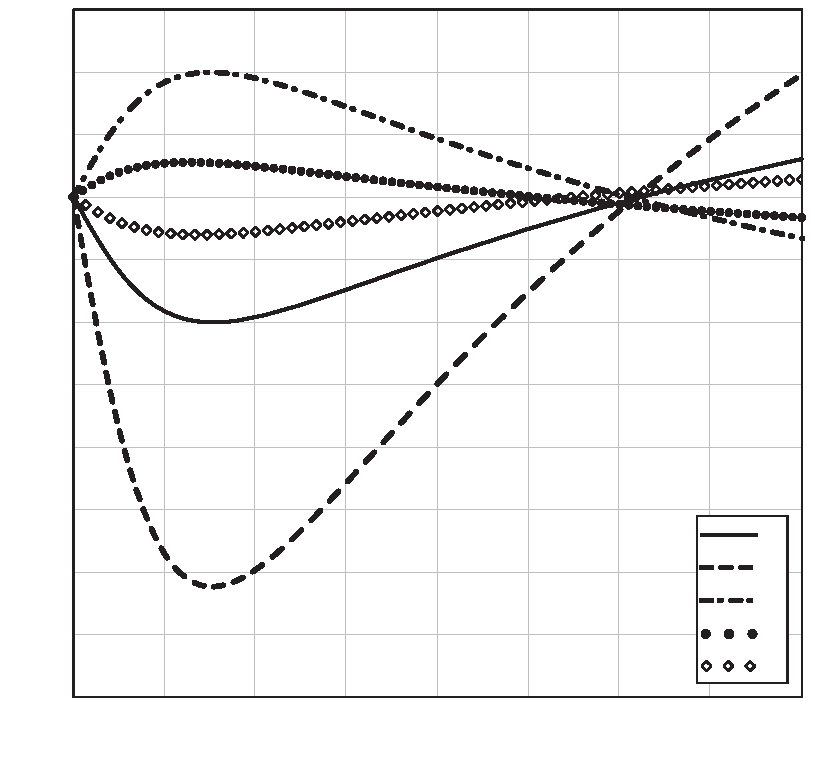
\includegraphics[width=\unitlength]{sigma_ot_h_rus.pdf}}%
        \put(0.08055673,0.15171806){\color[named]{black}\makebox(0,0)[rb]{\smash{$ - $7}}}%
        \put(0.08055673,0.22857968){\color[named]{black}\makebox(0,0)[rb]{\smash{$ - $6}}}%
        \put(0.08055673,0.3054413){\color[named]{black}\makebox(0,0)[rb]{\smash{$ - $5}}}%
        \put(0.08055673,0.38230285){\color[named]{black}\makebox(0,0)[rb]{\smash{$ - $4}}}%
        \put(0.08055673,0.45916447){\color[named]{black}\makebox(0,0)[rb]{\smash{$ - $3}}}%
        \put(0.08055673,0.53602609){\color[named]{black}\makebox(0,0)[rb]{\smash{$ - $2}}}%
        \put(0.08055673,0.61288771){\color[named]{black}\makebox(0,0)[rb]{\smash{$ - $1}}}%
        \put(0.08055673,0.68974934){\color[named]{black}\makebox(0,0)[rb]{\smash{0}}}%
        \put(0.08055673,0.76661096){\color[named]{black}\makebox(0,0)[rb]{\smash{1}}}%
        \put(0.08055673,0.84347258){\color[named]{black}\makebox(0,0)[rb]{\smash{2}}}%
        \put(0.08055673,0.9203342){\color[named]{black}\makebox(0,0)[rb]{\smash{3}}}%
        \put(0.94177486,0.27828351){\color[named]{black}\makebox(0,0)[lb]{\smash{\textsl{1}}}}%
        \put(0.94177486,0.23800802){\color[named]{black}\makebox(0,0)[lb]{\smash{\textsl{2}}}}%
        \put(0.94177486,0.19757881){\color[named]{black}\makebox(0,0)[lb]{\smash{\textsl{3}}}}%
        \put(0.94177486,0.15730331){\color[named]{black}\makebox(0,0)[lb]{\smash{\textsl{4}}}}%
        \put(0.08992072,0.05199177){\color[named]{black}\makebox(0,0)[lb]{\smash{0}}}%
        \put(0.19056419,0.05199177){\color[named]{black}\makebox(0,0)[lb]{\smash{0,5}}}%
        \put(0.31327655,0.05199177){\color[named]{black}\makebox(0,0)[lb]{\smash{1}}}%
        \put(0.4123701,0.05199177){\color[named]{black}\makebox(0,0)[lb]{\smash{1,5}}}%
        \put(0.5368076,0.05199177){\color[named]{black}\makebox(0,0)[lb]{\smash{2}}}%
        \put(0.63734594,0.05199177){\color[named]{black}\makebox(0,0)[lb]{\smash{2,5}}}%
        \put(0.76046997,0.05199177){\color[named]{black}\makebox(0,0)[lb]{\smash{3}}}%
        \put(0.86026396,0.05199177){\color[named]{black}\makebox(0,0)[lb]{\smash{3,5}}}%
        \put(0.98330909,0.05199177){\color[named]{black}\makebox(0,0)[lb]{\smash{4}}}%
        \put(0.53839145,-0.00000007){\color[named]{black}\makebox(0,0)[b]{\smash{$ H $}}}%
        \put(0.01490498,0.51027967){\color[named]{black}\rotatebox{90}{\makebox(0,0)[b]{\smash{$\sigma_x^T$, МПа}}}}%
        \put(0.08055673,0.07793062){\color[named]{black}\makebox(0,0)[rb]{\smash{\textsl{$-$}8}}}%
        \put(0.94177486,0.11631029){\color[named]{black}\makebox(0,0)[lb]{\smash{\textsl{5}}}}%
      \end{picture}%
    \endgroup%

    \caption{Расчётные остаточные напряжения на свободной поверхности кремния в зависимости от отношения $ H $ толщины стекла к толщине кремния для рабочей температуры $T_w$~=~20~{\textdegree}C и температуры соединения $ T_b $ =~350~{\textdegree}C:}
    \label{fig:sigma_ot_h_rus}
    \textsl{1} "--- Corning 7740,  \textsl{2} "--- Schott Borofloat 33,  \textsl{3} "--- ЛК5,  \textsl{4} "--- Hoya~SD-2, \textsl{5}~---~Asahi~SW\nb-YY%
\end{figure}



\begin{table} [!hb]
    \centering%
	\caption{Расчётное значение оптимального отношения толщины стекла
	к~толщине кремния (для неструктурированных материалов)}%
	\label{tab_h0_stekla}% label всегда желательно идти после caption
    \renewcommand{\arraystretch}{1.3}%% Увеличение расстояния между рядами, для улучшения восприятия.
	\def\tabularxcolumn#1{m{#1}}
	\begin{SingleSpace}
	\begin{tabular}{@{}lc}
        \toprule     %%% верхняя линейка
        Марка стекла &
        $H_0$\\
        \midrule
        Corning 7740 &
        3,12\\
        Schott Borofloat 33 &
        3,09\\
        ЛК5 &
        3,05\\
        Asahi SW\nobreakdash-YY &
        2,76\\
        Hoya SD\nobreakdash-2 &
        2,54\\
        \bottomrule %%% нижняя линейка
	\end{tabular}%
	\end{SingleSpace}
\end{table}

Если учитывать температурную зависимость модуля Юнга материалов, то~однозначно говорить о наличии наиболее оптимальной толщины стекла нельзя.
Для определения оптимальной толщины нужно рассматривать каждую конкретную комбинацию стекла и кремния с учётом всех допустимых диапазонов температур соединения и их влияния на напряжения в рабочем диапазоне.
При~этом может быть найден узкий диапазон соотношений толщин стекла и~кремния, удовлетворяющий целям оптимизации.
Для повышения качества оценки в этом случае следует подобрать такую расчётную модель, которая бы~позволила без дополнительных усложнений расчётов учитывать температурную зависимость жёсткости.

\begin{figure}[!htb]
    \centering
    \begingroup%
      \makeatletter%
      \providecommand\color[2][]{%
        \errmessage{(Inkscape) Color is used for the text in Inkscape, but the package 'color.sty' is not loaded}%
        \renewcommand\color[2][]{}%
      }%
      \providecommand\transparent[1]{%
        \errmessage{(Inkscape) Transparency is used (non-zero) for the text in Inkscape, but the package 'transparent.sty' is not loaded}%
        \renewcommand\transparent[1]{}%
      }%
      \providecommand\rotatebox[2]{#2}%
      \ifx\svgwidth\undefined%
        \setlength{\unitlength}{0.75\textwidth}%
        \ifx\svgscale\undefined%
          \relax%
        \else%
          \setlength{\unitlength}{\unitlength * \real{\svgscale}}%
        \fi%
      \else%
        \setlength{\unitlength}{\svgwidth}%
      \fi%
      \global\let\svgwidth\undefined%
      \global\let\svgscale\undefined%
      \makeatother%
      \begin{picture}(1,0.94457378)%
        \put(0,0){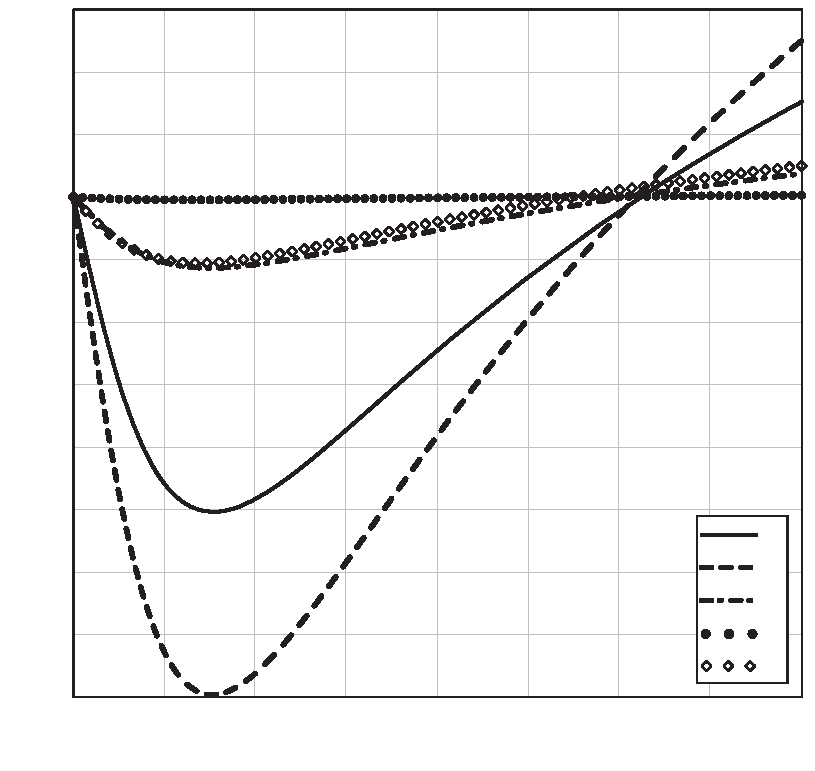
\includegraphics[width=\unitlength]{sigma_ot_h85_rus.pdf}}%
        \put(0.08055675,0.15171806){\color[named]{black}\makebox(0,0)[rb]{\smash{$-$7}}}%
        \put(0.08055675,0.22857969){\color[named]{black}\makebox(0,0)[rb]{\smash{$-$6}}}%
        \put(0.08055675,0.30544124){\color[named]{black}\makebox(0,0)[rb]{\smash{$-$5}}}%
        \put(0.08055675,0.38230295){\color[named]{black}\makebox(0,0)[rb]{\smash{$-$4}}}%
        \put(0.08055675,0.45916457){\color[named]{black}\makebox(0,0)[rb]{\smash{$-$3}}}%
        \put(0.08055675,0.5360262){\color[named]{black}\makebox(0,0)[rb]{\smash{$-$2}}}%
        \put(0.08055675,0.61288783){\color[named]{black}\makebox(0,0)[rb]{\smash{$-$1}}}%
        \put(0.08055675,0.68974946){\color[named]{black}\makebox(0,0)[rb]{\smash{0}}}%
        \put(0.08055675,0.76661108){\color[named]{black}\makebox(0,0)[rb]{\smash{1}}}%
        \put(0.08055675,0.84347271){\color[named]{black}\makebox(0,0)[rb]{\smash{2}}}%
        \put(0.08055675,0.92033434){\color[named]{black}\makebox(0,0)[rb]{\smash{3}}}%
        \put(0.94177492,0.27828353){\color[named]{black}\makebox(0,0)[lb]{\smash{\textsl{1}}}}%
        \put(0.94177492,0.23800803){\color[named]{black}\makebox(0,0)[lb]{\smash{\textsl{2}}}}%
        \put(0.94177492,0.19757882){\color[named]{black}\makebox(0,0)[lb]{\smash{\textsl{3}}}}%
        \put(0.94177492,0.15730332){\color[named]{black}\makebox(0,0)[lb]{\smash{\textsl{4}}}}%
        \put(0.08992074,0.05199178){\color[named]{black}\makebox(0,0)[lb]{\smash{0}}}%
        \put(0.19056421,0.05199178){\color[named]{black}\makebox(0,0)[lb]{\smash{0,5}}}%
        \put(0.31327658,0.05199178){\color[named]{black}\makebox(0,0)[lb]{\smash{1}}}%
        \put(0.41237014,0.05199178){\color[named]{black}\makebox(0,0)[lb]{\smash{1,5}}}%
        \put(0.53680764,0.05199178){\color[named]{black}\makebox(0,0)[lb]{\smash{2}}}%
        \put(0.63734607,0.05199178){\color[named]{black}\makebox(0,0)[lb]{\smash{2,5}}}%
        \put(0.76047002,0.05199178){\color[named]{black}\makebox(0,0)[lb]{\smash{3}}}%
        \put(0.86026402,0.05199178){\color[named]{black}\makebox(0,0)[lb]{\smash{3,5}}}%
        \put(0.98330916,0.05199178){\color[named]{black}\makebox(0,0)[lb]{\smash{4}}}%
        \put(0.53839149,-0.00000007){\color[named]{black}\makebox(0,0)[b]{\smash{$ H $}}}%
        \put(0.01490501,0.51027978){\color[named]{black}\rotatebox{90}{\makebox(0,0)[b]{\smash{$\sigma_x^T$, МПа}}}}%
        \put(0.08055675,0.07793062){\color[named]{black}\makebox(0,0)[rb]{\smash{$-$8}}}%
        \put(0.94177492,0.1163103){\color[named]{black}\makebox(0,0)[lb]{\smash{\textsl{5}}}}%
      \end{picture}%
    \endgroup%

    \caption{Расчётные остаточные напряжения на свободной поверхности кремния в зависимости от отношения $ H $ толщины стекла к толщине кремния для случая рабочей температуры $T_w$~=~85~{\textdegree}C и температуры соединения $T_b=$~350~{\textdegree}C:}
    \label{fig:sigma_ot_h85_rus}
    \textsl{1} "--- Corning 7740,  \textsl{2} "--- Schott Borofloat 33,  \textsl{3} "--- ЛК5,  \textsl{4} "--- Hoya~SD-2,  \textsl{5}~---~Asahi~SW\nb-YY%
\end{figure}

\subsection[Оценка напряжений в сборках стекло---кремний---стекло]{Оценка напряжений в сборках стекло"--~кремний"--~стекло}

На Рисунке~\ref{fig:sigma_z_gsg_lk5} представлен график распределения остаточных напряжений в сборке при рабочей температуре 20~{\textdegree}C (температура соединения 310~{\textdegree}C), рассчитанный по модели многослойного композиционного материала для случая трёхслойной модели стекло"--~кремний"--~стекло. Марка стекла, использованная в расчёте "--- ЛК5. За плоскость отсчёта координаты по оси z взята срединная плоскость пластины кремния. Толщина пластины кремния равна 0,46~мм, толщина пластин стекла равна 0,6~мм. В симметричных структурах, как, например, стекло-кремний-стекло, соединённых при единой температуре, согласно применённой модели напряжения постоянны по толщине слоёв. Причиной тому являются допущения применяемой модели расчёта.

\begin{figure}[!htb]
    \centering
    \begingroup%
     \makeatletter%
      \providecommand\color[2][]{%
        \errmessage{(Inkscape) Color is used for the text in Inkscape, but the package 'color.sty' is not loaded}%
        \renewcommand\color[2][]{}%
      }%
      \providecommand\transparent[1]{%
        \errmessage{(Inkscape) Transparency is used (non-zero) for the text in Inkscape, but the package 'transparent.sty' is not loaded}%
        \renewcommand\transparent[1]{}%
      }%
      \providecommand\rotatebox[2]{#2}%
      \ifx\svgwidth\undefined%
        \setlength{\unitlength}{0.5\textwidth}%
        \ifx\svgscale\undefined%
          \relax%
        \else%
          \setlength{\unitlength}{\unitlength * \real{\svgscale}}%
        \fi%
      \else%
        \setlength{\unitlength}{\svgwidth}%
      \fi%
      \global\let\svgwidth\undefined%
      \global\let\svgscale\undefined%
      \makeatother%
      \begin{picture}(1,0.79291385)%
        \put(0,0){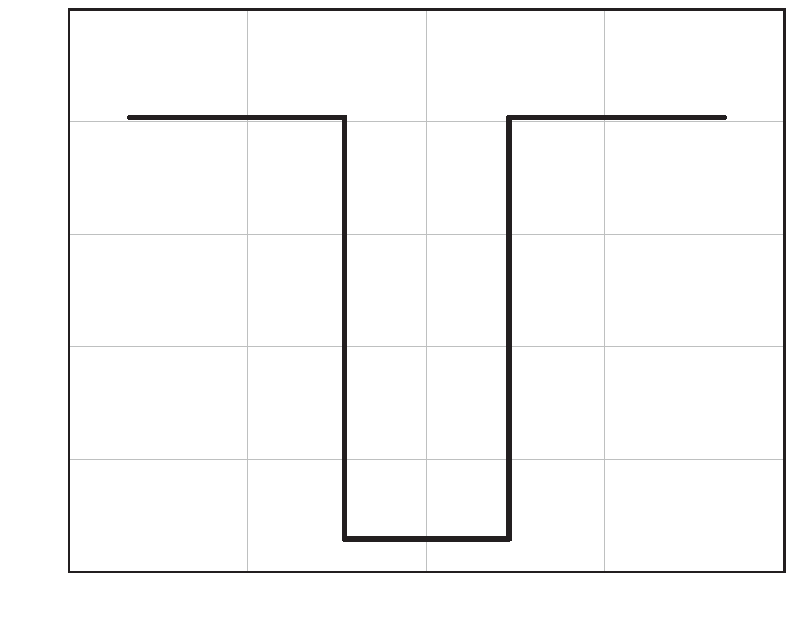
\includegraphics[width=\unitlength]{sigma_z_gsg_lk5.pdf}}%
        \put(0.11408864,0.04336622){\color[named]{black}\makebox(0,0)[rb]{\smash{$-$1}}}%
        \put(0.34892102,0.04336622){\color[named]{black}\makebox(0,0)[rb]{\smash{$-$0,5}}}%
        \put(0.54767302,0.04336622){\color[named]{black}\makebox(0,0)[rb]{\smash{0}}}%
        \put(0.79909406,0.04336622){\color[named]{black}\makebox(0,0)[rb]{\smash{0,5}}}%
        \put(1.0044296,0.04336622){\color[named]{black}\makebox(0,0)[rb]{\smash{1}}}%
        \put(0.07054353,0.07167086){\color[named]{black}\makebox(0,0)[rb]{\smash{$-$5}}}%
        \put(0.07054353,0.20852634){\color[named]{black}\makebox(0,0)[rb]{\smash{$-$4}}}%
        \put(0.07054353,0.34849261){\color[named]{black}\makebox(0,0)[rb]{\smash{$-$2}}}%
        \put(0.07054353,0.48845887){\color[named]{black}\makebox(0,0)[rb]{\smash{0}}}%
        \put(0.07054353,0.62842514){\color[named]{black}\makebox(0,0)[rb]{\smash{2}}}%
        \put(0.07054353,0.7683914){\color[named]{black}\makebox(0,0)[rb]{\smash{4}}}%
        \put(-0.05,0.43130823){\color[named]{black}\rotatebox{90}{\makebox(0,0)[b]{\smash{$\sigma_x^T$, МПа}}}}%
        \put(0.53103509,0.00604198){\color[named]{black}\makebox(0,0)[b]{\smash{$z$, мм}}}%
      \end{picture}%
    \endgroup%

    \caption{Расчётный график распределения остаточных напряжений при рабочей температуре 20~{\textdegree}C (температура соединения 310~{\textdegree}C) в сборке стекло-кремний-стекло, где кремний толщиной 0,46 мм и стекло ЛК5 толщиной 0,6 мм}
    \label{fig:sigma_z_gsg_lk5}
\end{figure}

\section{Моделирование методом конечных элементов}
На основе исходных данных по свойствам материалов, описанных
в подразделе \ref{chap_source_data}, было проведено моделирование
методом конечных элементов. Использовалось программное обеспечение
CoventorWare Turbo 2012, которое в своей расчётной части опирается
на универсальную систему конечно-элементного анализа Abaqus 6.9.
Эти результаты и особенности моделирования можно распространить
на~прочие программы и~комплексы конечно-элементного моделирования.

\subsection{Задание температурной зависимости температурного коэффициента линейного расширения в~программах конечно-элементного моделирования}

Согласно инструкции для пользователя CoventorWare Turbo 2012 температурную
зависимость истинного температурного
коэффициента линейного расширения необходимо задавать в интегральной форме
вместо дифференциальной, приводимой в большинстве литературных источников,
а~также в~данной работе. Для такой формы представления важно знать пределы
интегрирования, в первую очередь температуру начала интегрирования. Для случая
анодной посадки это будет температура соединения \(T_b\).

Приведение записи ТКЛР в дифференциальной форме к записи в интегральной форме
производится согласно следующей формуле:
\begin{equation}
    \alpha^\mathrm{int}(T_w, T_b) =
    \int\limits_{T_b}^{T_w}
    \frac{1}{T_w-T_b}
    \alpha^\mathrm{dif}(T)\:\mathrm{d}T
\end{equation}

После такого преобразования зависимость ТКЛР, представленная
в~дифференциальной форме полиномом вида \eqref{eq:polynom_sample}, будет
выражаться полиномом того же порядка вида
\begin{multline}
    \alpha^\mathrm{int}(T_w, T_b) =
    \left(a + \frac{b}{2} \cdot T_b + \frac{c}{3} \cdot T_b^2 + \frac{d}{4} \cdot T_b^3 + \frac{e}{5} \cdot T_b^4\right)
    + \\ +
    \left(\frac{b}{2} + \frac{c}{3} \cdot T_b + \frac{d}{4} \cdot T_b^2 + \frac{e}{5} \cdot T_b^3\right) \cdot T_w
    + % \\ +
    \left(\frac{c}{3}+\frac{d}{4} \cdot T_b + \frac{e}{5} \cdot T_b^2\right) \cdot T_w^2
    + \\ +
    \left(\frac{d}{4} + \frac{e}{5} \cdot T_b\right) \cdot T_w^3 +
    \frac{e}{5} \cdot T_w^4
\end{multline}

Автоматизация преобразования полиномов возможна
при помощи следующей программы на языке \verb|R|:
\begin{Verb}
cteIntFormCoef <-
  function(coeforig = c(0, 1),
           temperature0 = 273.15) {
    a <- as.numeric(coeforig)
    coefresult <- a
    la <- length(a)
    for (i in la:1) {
      if (i == la)
        coefresult[i] <- a[i] / i
      if (i != la)
        coefresult[i] <- a[i] / i + coefresult[i + 1] * temperature0
    }
    coefresult
  }
\end{Verb}

\subsection{Результаты моделирования}

На Рисунке~\ref{fig:stressX_distrib} показан результат моделирования конечными
элементами распределения напряжений в соединённых пластинах кремния и стекла.
Использовалась модель из двух соединённых пластин диаметром 100 мм:
кремний толщиной 460 мкм и стекло толщиной 600 мкм.
ТКЛР материалов модели устанавливались с использованием возможности задать
температуру, при которой в~материале отсутствуют напряжения.
Эта температура задавалась равной температуре соединения $T_b$.
Граничное условие температуры моделируемых объёмов задавалось равным рабочей температуре $T_w$.

\begin{figure}[!hbt]
    \centering
    \ifdefmacro{\tikzsetnextfilename}{\tikzsetnextfilename{stressX_distrib}}{}%
    % Created by tikzDevice version 0.10.1 on 2016-09-27 23:29:32
% !TEX encoding = UTF-8 Unicode
\begin{tikzpicture}[x=1pt,y=1pt]
\definecolor{fillColor}{RGB}{255,255,255}
\path[use as bounding box,fill=fillColor] (0,0) rectangle (284.53,170.72);
\begin{scope}
\path[clip] (  0.00,  0.00) rectangle (284.53,170.72);
\definecolor{drawColor}{RGB}{255,255,255}

\path[draw=drawColor,line width= 0.6pt,line join=round,line cap=round,fill=fillColor] (  0.00,  0.00) rectangle (284.53,170.72);
\end{scope}
\begin{scope}
\path[clip] ( 40.77, 32.43) rectangle (284.53,170.72);
\definecolor{fillColor}{RGB}{255,255,255}

\path[fill=fillColor] ( 40.77, 32.43) rectangle (284.53,170.72);
\definecolor{drawColor}{gray}{0.98}

\path[draw=drawColor,line width= 0.6pt,line join=round] ( 40.77, 54.61) --
	(284.53, 54.61);

\path[draw=drawColor,line width= 0.6pt,line join=round] ( 40.77, 95.11) --
	(284.53, 95.11);

\path[draw=drawColor,line width= 0.6pt,line join=round] ( 40.77,135.61) --
	(284.53,135.61);

\path[draw=drawColor,line width= 0.6pt,line join=round] ( 53.94, 32.43) --
	( 53.94,170.72);

\path[draw=drawColor,line width= 0.6pt,line join=round] (116.65, 32.43) --
	(116.65,170.72);

\path[draw=drawColor,line width= 0.6pt,line join=round] (179.37, 32.43) --
	(179.37,170.72);

\path[draw=drawColor,line width= 0.6pt,line join=round] (242.09, 32.43) --
	(242.09,170.72);
\definecolor{drawColor}{gray}{0.90}

\path[draw=drawColor,line width= 0.2pt,line join=round] ( 40.77, 34.36) --
	(284.53, 34.36);

\path[draw=drawColor,line width= 0.2pt,line join=round] ( 40.77, 74.86) --
	(284.53, 74.86);

\path[draw=drawColor,line width= 0.2pt,line join=round] ( 40.77,115.36) --
	(284.53,115.36);

\path[draw=drawColor,line width= 0.2pt,line join=round] ( 40.77,155.87) --
	(284.53,155.87);

\path[draw=drawColor,line width= 0.2pt,line join=round] ( 85.30, 32.43) --
	( 85.30,170.72);

\path[draw=drawColor,line width= 0.2pt,line join=round] (148.01, 32.43) --
	(148.01,170.72);

\path[draw=drawColor,line width= 0.2pt,line join=round] (210.73, 32.43) --
	(210.73,170.72);

\path[draw=drawColor,line width= 0.2pt,line join=round] (273.45, 32.43) --
	(273.45,170.72);
\definecolor{drawColor}{RGB}{0,0,0}

\path[draw=drawColor,line width= 1.3pt,line join=round] ( 51.85,157.39) --
	( 99.93, 98.07) --
	(148.01, 38.72) --
	(148.01,164.43) --
	(160.56,157.29) --
	(173.10,150.15) --
	(185.64,143.00) --
	(198.19,135.86) --
	(210.73,128.71) --
	(223.27,121.56) --
	(235.82,114.42) --
	(248.36,107.27) --
	(260.90,100.12) --
	(273.45, 92.97);

\path[draw=drawColor,line width= 0.9pt,line join=round,line cap=round] ( 40.77, 32.43) rectangle (284.53,170.72);
\end{scope}
\begin{scope}
\path[clip] (  0.00,  0.00) rectangle (284.53,170.72);
\definecolor{drawColor}{RGB}{0,0,0}

\node[text=drawColor,anchor=base east,inner sep=0pt, outer sep=0pt, scale=  1.00] at ( 35.37, 29.40) {\(-4\)};

\node[text=drawColor,anchor=base east,inner sep=0pt, outer sep=0pt, scale=  1.00] at ( 35.37, 69.90) {\(-2\)};

\node[text=drawColor,anchor=base east,inner sep=0pt, outer sep=0pt, scale=  1.00] at ( 35.37,110.40) {\(0\)};

\node[text=drawColor,anchor=base east,inner sep=0pt, outer sep=0pt, scale=  1.00] at ( 35.37,150.91) {\(2\)};
\end{scope}
\begin{scope}
\path[clip] (  0.00,  0.00) rectangle (284.53,170.72);
\definecolor{drawColor}{RGB}{0,0,0}

\path[draw=drawColor,line width= 0.6pt,line join=round] ( 37.77, 34.36) --
	( 40.77, 34.36);

\path[draw=drawColor,line width= 0.6pt,line join=round] ( 37.77, 74.86) --
	( 40.77, 74.86);

\path[draw=drawColor,line width= 0.6pt,line join=round] ( 37.77,115.36) --
	( 40.77,115.36);

\path[draw=drawColor,line width= 0.6pt,line join=round] ( 37.77,155.87) --
	( 40.77,155.87);
\end{scope}
\begin{scope}
\path[clip] (  0.00,  0.00) rectangle (284.53,170.72);
\definecolor{drawColor}{RGB}{0,0,0}

\path[draw=drawColor,line width= 0.6pt,line join=round] ( 85.30, 29.43) --
	( 85.30, 32.43);

\path[draw=drawColor,line width= 0.6pt,line join=round] (148.01, 29.43) --
	(148.01, 32.43);

\path[draw=drawColor,line width= 0.6pt,line join=round] (210.73, 29.43) --
	(210.73, 32.43);

\path[draw=drawColor,line width= 0.6pt,line join=round] (273.45, 29.43) --
	(273.45, 32.43);
\end{scope}
\begin{scope}
\path[clip] (  0.00,  0.00) rectangle (284.53,170.72);
\definecolor{drawColor}{RGB}{0,0,0}

\node[text=drawColor,anchor=base,inner sep=0pt, outer sep=0pt, scale=  1.00] at ( 85.30, 17.12) {\(-300\)};

\node[text=drawColor,anchor=base,inner sep=0pt, outer sep=0pt, scale=  1.00] at (148.01, 17.12) {\(0\)};

\node[text=drawColor,anchor=base,inner sep=0pt, outer sep=0pt, scale=  1.00] at (210.73, 17.12) {\(300\)};

\node[text=drawColor,anchor=base,inner sep=0pt, outer sep=0pt, scale=  1.00] at (273.45, 17.12) {\(600\)};
\end{scope}
\begin{scope}
\path[clip] (  0.00,  0.00) rectangle (284.53,170.72);
\definecolor{drawColor}{RGB}{0,0,0}

\node[text=drawColor,anchor=base,inner sep=0pt, outer sep=0pt, scale=  1.00] at (162.65,  2.40) {\(z\), мкм};
\end{scope}
\begin{scope}
\path[clip] (  0.00,  0.00) rectangle (284.53,170.72);
\definecolor{drawColor}{RGB}{0,0,0}

\node[text=drawColor,rotate= 90.00,anchor=base,inner sep=0pt, outer sep=0pt, scale=  1.00] at ( 12.32,101.57) {\(\sigma_x^T\), МПа};
\end{scope}
\end{tikzpicture}
%

    \caption{Распределение остаточных напряжений
    при $T_w$ = 20~{\textdegree}C  в~сборке
    кремния толщиной 460 мкм и стекла ЛК5 толщиной 600 мкм,
    соединёнными при температуре $T_b$ = 300~{\textdegree}C, смоделированное
    в~программе конечно-элементного моделирования}
    \label{fig:stressX_distrib}
\end{figure}

Моделирование методом конечных элементов в комплексе для моделирования МЭМС
Coventorware Turbo подтвердило форму эпюр расчётных напряжений.

На Рисунках~\ref{fig:si_membrane_bonded_3d}
и~\ref{fig:si_membrane_third_inv_stress} показаны результаты  моделирования
конечными элементами сборки кремниевого элемента размерами
4\(\,\times\,\)4\(\,\times\,\)0,46~мм с структурированным элементом толщиной 50~мкм
и стеклянного элемента размерами
4\(\,\times\,\)4\(\,\times\,\)0,6~мм. Площадь области соединения со стеклом
составляет половину от площади поверхности стеклянного элемента. Температура
проведения смоделированного соединения 300~{\textdegree}C. Марка стекла "---
ЛК5.

Видно, что в данном случае также существует оптимальная толщина стекла,
описанная в подразделе~\ref{chap_optim_glass_thickness}, минимизирующая
остаточные напряжения на поверхности кремния. Отношение оптимальной толщины
стекла к~толщине кремния в данной модели примерно в два раза меньше, чем
представлено ранее на Рисунке~\ref{fig:glass_stress_multilayer_ot_h_tw} на
странице~\pageref{fig:glass_stress_multilayer_ot_h_tw}, поскольку площадь соединения с
поверхностью стекла в два раза меньше, чем было бы в случае отсутствия
структуры, сформированной вытравливанием кремния.

\begin{figure}[!hb]
    \centering
    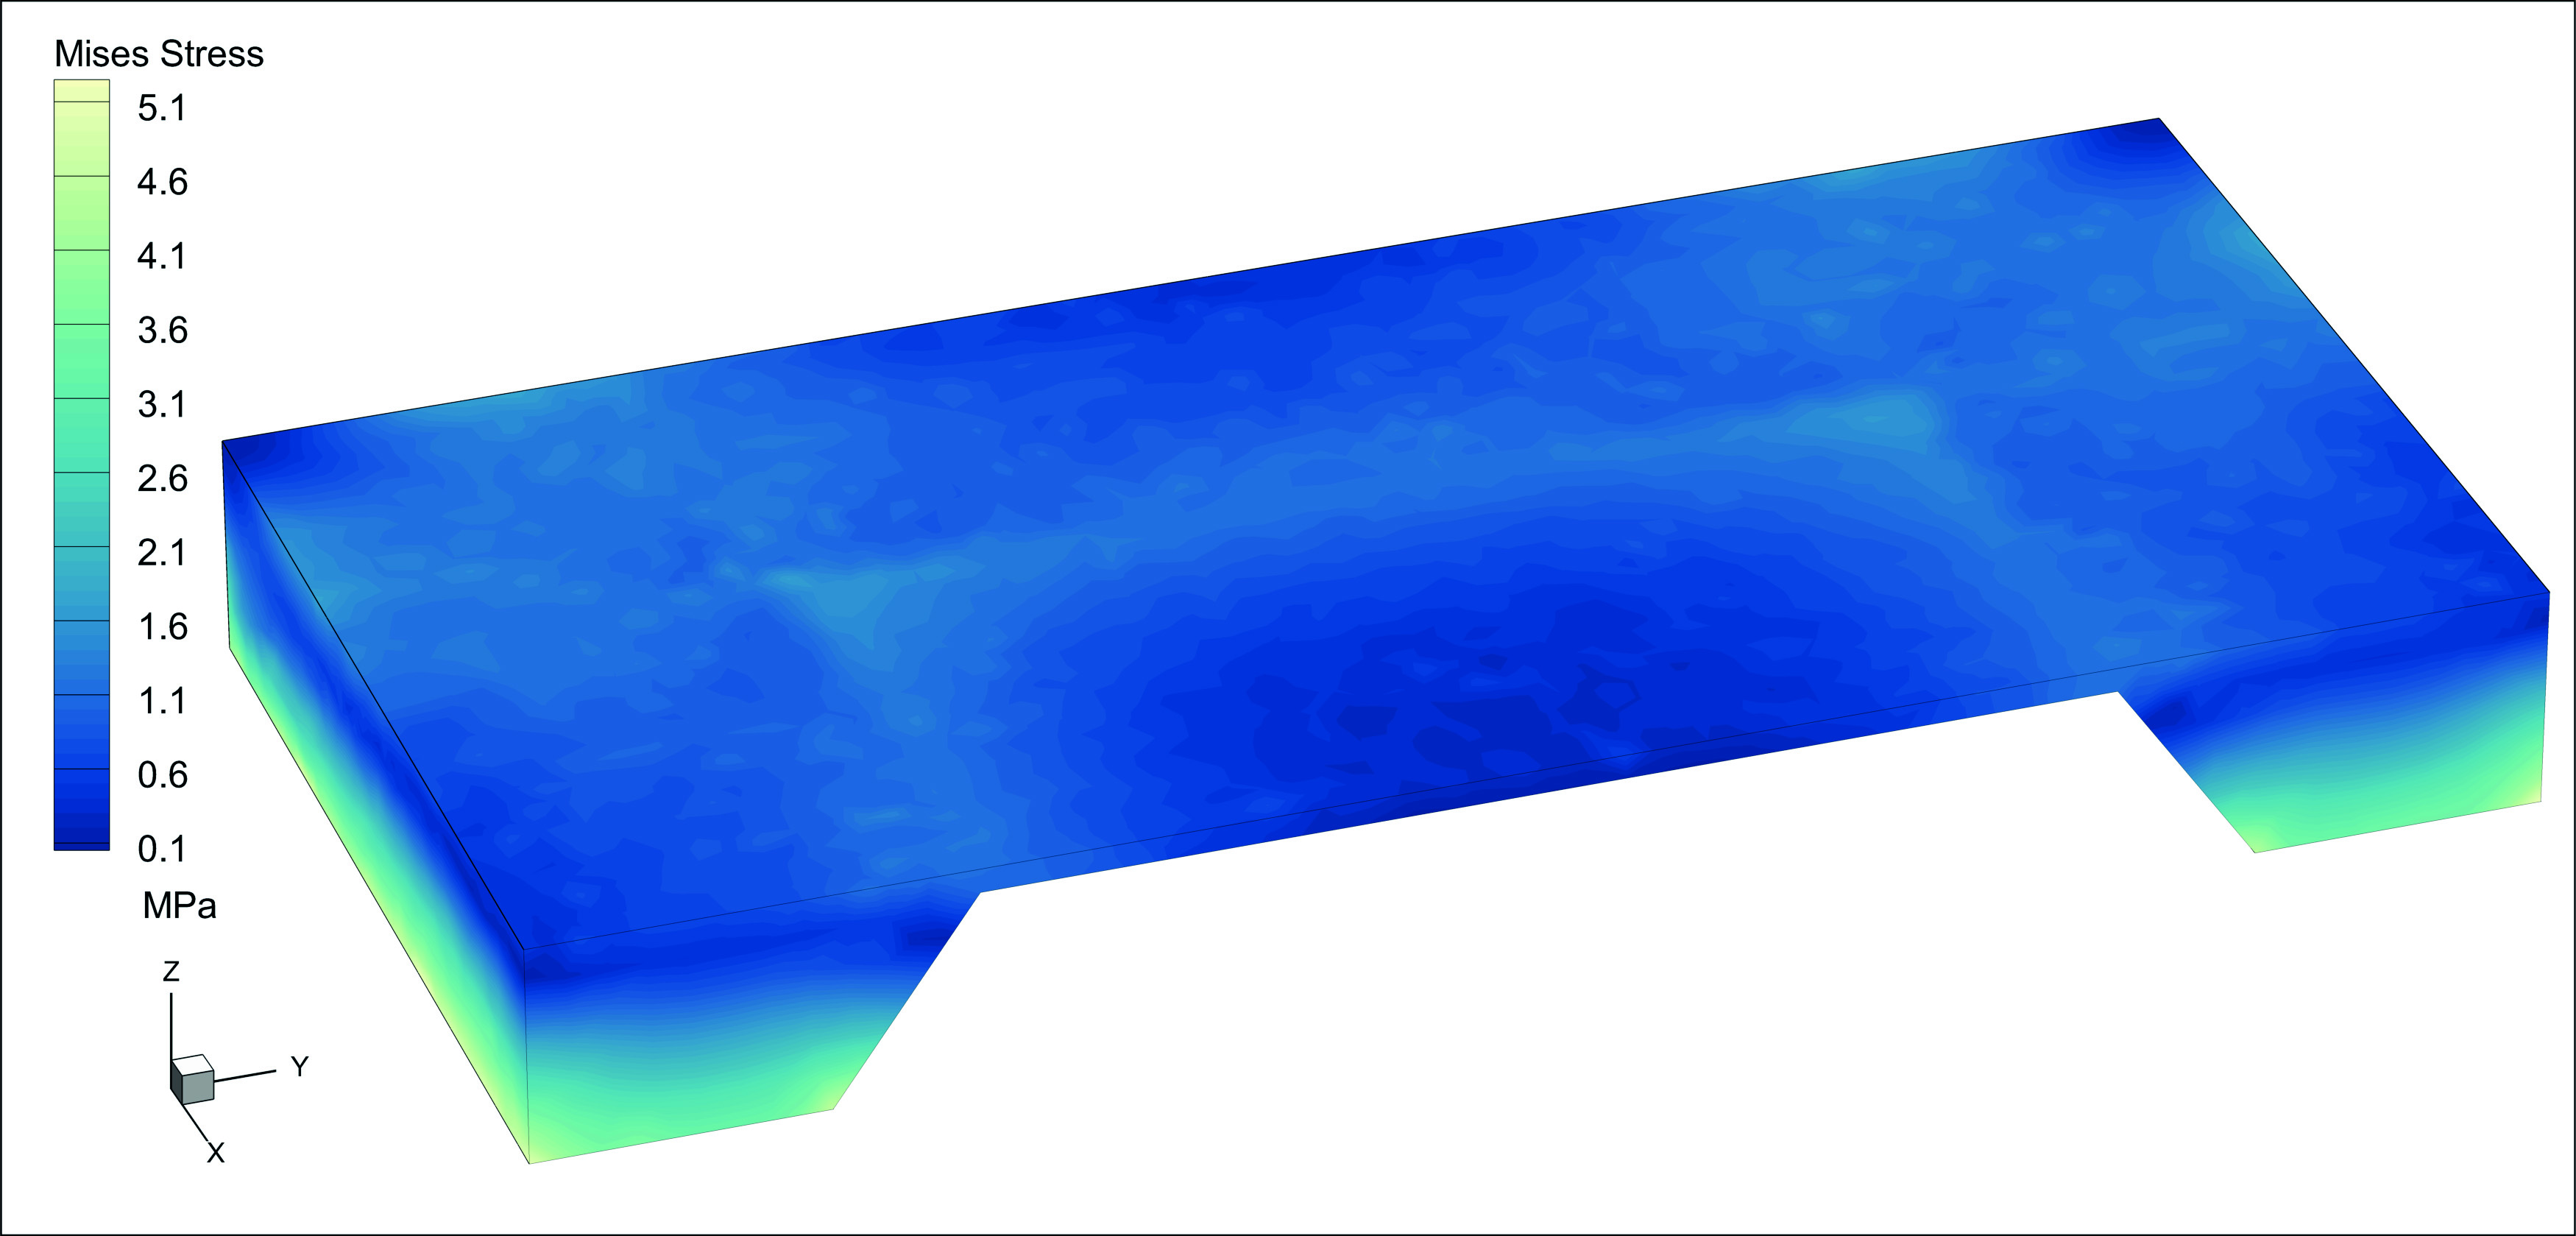
\includegraphics[height=0.2\textheight]{b300chip_lk5_st460gt460mask0,5mem50_stress@20+gtcoef_step4arb.jpg}\par%
    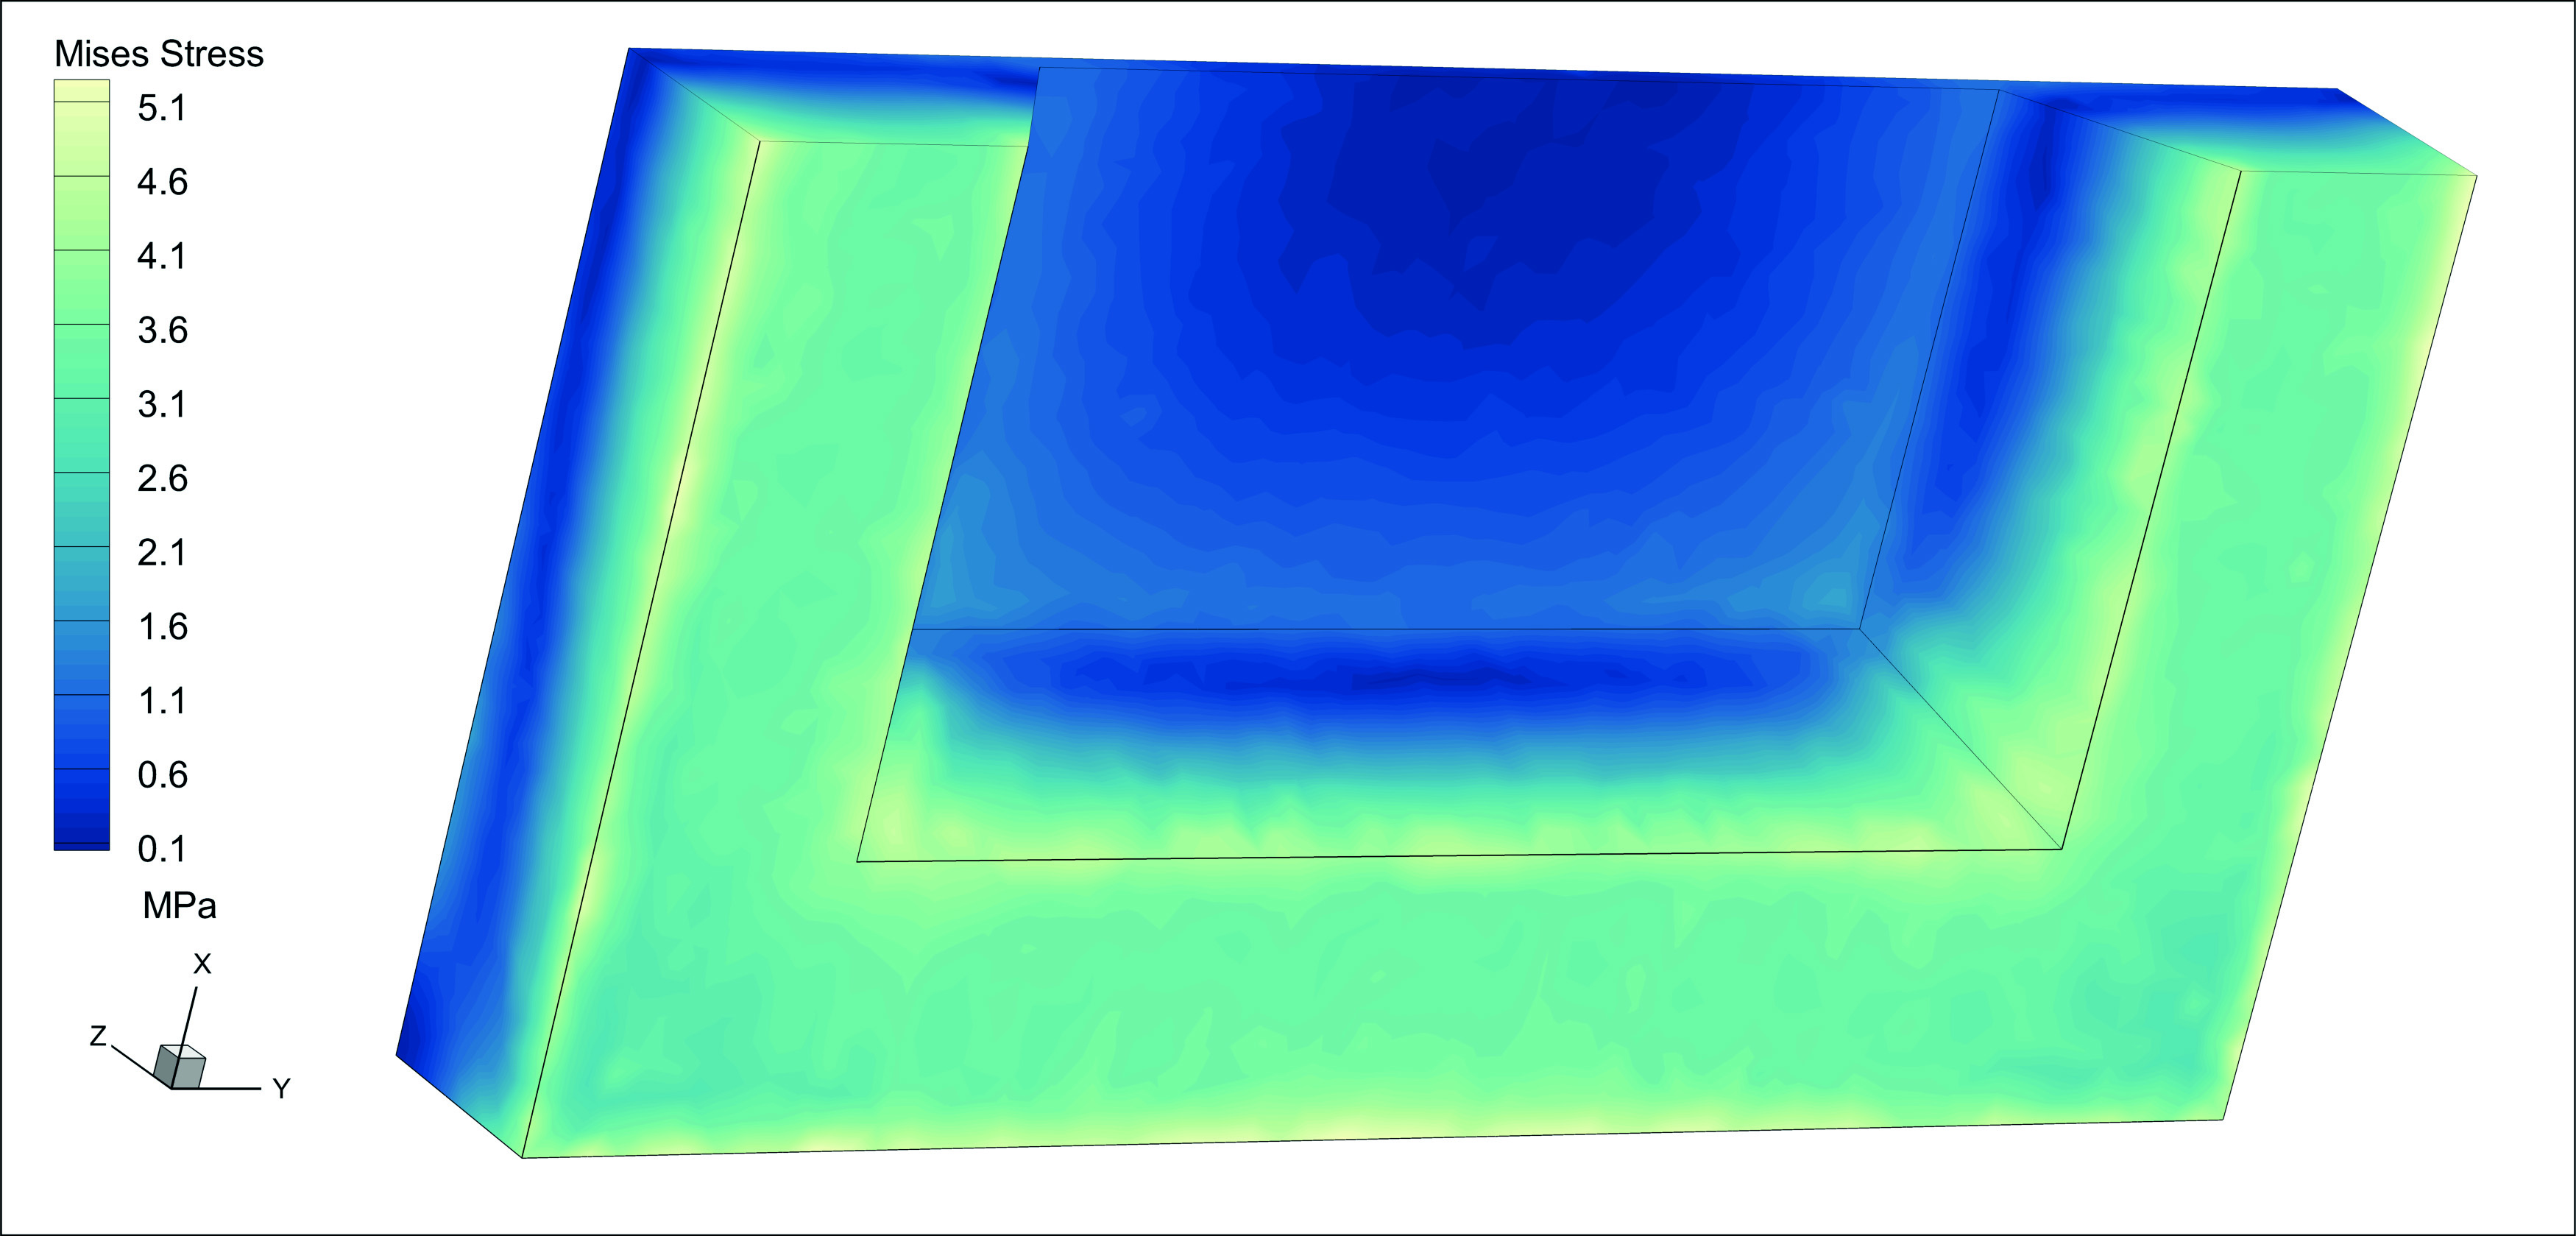
\includegraphics[height=0.2\textheight]{b300chip_lk5_st460gt460mask0,5mem50_stress@20+gtcoef_step4xy.jpg}%

    \caption{Смоделированная картина распределения напряжений
    в~структурированном кремнии после анодной посадки на стекло ЛК5}
    \label{fig:si_membrane_bonded_3d}
\end{figure}

\begin{figure}[!hb]
    \hspace{1.5em}%
    \ifdefmacro{\tikzsetnextfilename}{\tikzsetnextfilename{si_membrane_third_inv_stress}}{}%
    \begin{tikzpicture}[x=1pt,y=1pt]
\definecolor{fillColor}{RGB}{255,255,255}
\path[use as bounding box,fill=fillColor] (0,0) rectangle (426.79,256.07);
\begin{scope}
\path[clip] (  0.00,  0.00) rectangle (426.79,256.07);
\definecolor{drawColor}{RGB}{255,255,255}

\path[draw=drawColor,line width= 0.6pt,line join=round,line cap=round,fill=fillColor] (  0.00,  0.00) rectangle (426.79,256.07);
\end{scope}
\begin{scope}
\path[clip] ( 36.22, 32.43) rectangle (426.79,242.11);
\definecolor{fillColor}{RGB}{255,255,255}

\path[fill=fillColor] ( 36.22, 32.43) rectangle (426.79,242.11);
\definecolor{drawColor}{gray}{0.98}

\path[draw=drawColor,line width= 0.6pt,line join=round] ( 36.22, 64.93) --
	(426.79, 64.93);

\path[draw=drawColor,line width= 0.6pt,line join=round] ( 36.22,132.24) --
	(426.79,132.24);

\path[draw=drawColor,line width= 0.6pt,line join=round] ( 36.22,199.55) --
	(426.79,199.55);

\path[draw=drawColor,line width= 0.6pt,line join=round] ( 73.00, 32.43) --
	( 73.00,242.11);

\path[draw=drawColor,line width= 0.6pt,line join=round] (104.70, 32.43) --
	(104.70,242.11);

\path[draw=drawColor,line width= 0.6pt,line join=round] (136.40, 32.43) --
	(136.40,242.11);

\path[draw=drawColor,line width= 0.6pt,line join=round] (187.12, 32.43) --
	(187.12,242.11);

\path[draw=drawColor,line width= 0.6pt,line join=round] (250.53, 32.43) --
	(250.53,242.11);

\path[draw=drawColor,line width= 0.6pt,line join=round] (313.93, 32.43) --
	(313.93,242.11);

\path[draw=drawColor,line width= 0.6pt,line join=round] (377.34, 32.43) --
	(377.34,242.11);
\definecolor{drawColor}{gray}{0.90}

\path[draw=drawColor,line width= 0.2pt,line join=round] ( 36.22, 98.59) --
	(426.79, 98.59);

\path[draw=drawColor,line width= 0.2pt,line join=round] ( 36.22,165.90) --
	(426.79,165.90);

\path[draw=drawColor,line width= 0.2pt,line join=round] ( 36.22,233.21) --
	(426.79,233.21);

\path[draw=drawColor,line width= 0.2pt,line join=round] ( 53.98, 32.43) --
	( 53.98,242.11);

\path[draw=drawColor,line width= 0.2pt,line join=round] ( 92.02, 32.43) --
	( 92.02,242.11);

\path[draw=drawColor,line width= 0.2pt,line join=round] (117.38, 32.43) --
	(117.38,242.11);

\path[draw=drawColor,line width= 0.2pt,line join=round] (155.42, 32.43) --
	(155.42,242.11);

\path[draw=drawColor,line width= 0.2pt,line join=round] (218.83, 32.43) --
	(218.83,242.11);

\path[draw=drawColor,line width= 0.2pt,line join=round] (282.23, 32.43) --
	(282.23,242.11);

\path[draw=drawColor,line width= 0.2pt,line join=round] (345.63, 32.43) --
	(345.63,242.11);

\path[draw=drawColor,line width= 0.2pt,line join=round] (409.04, 32.43) --
	(409.04,242.11);
\definecolor{drawColor}{RGB}{0,0,0}

\path[draw=drawColor,line width= 1.4pt,dash pattern=on 4pt off 4pt ,line join=round] ( 53.98, 41.96) --
	( 86.95, 64.32) --
	( 92.02, 70.56) --
	(104.70, 87.28) --
	(117.38,100.68) --
	(123.72,109.64) --
	(168.10,155.99) --
	(180.78,165.96) --
	(193.47,174.76) --
	(206.15,182.50) --
	(218.83,189.32) --
	(282.23,212.97) --
	(409.04,232.58);

\path[draw=drawColor,line width= 1.4pt,line join=round] ( 53.98, 79.84) --
	( 86.95, 87.25) --
	( 92.02, 89.32) --
	(104.70, 94.86) --
	(117.38, 99.29) --
	(123.72,102.27) --
	(168.10,117.61) --
	(180.78,120.92) --
	(193.47,123.83) --
	(206.15,126.40) --
	(218.83,128.66) --
	(282.23,136.48) --
	(409.04,142.99);

\path[draw=drawColor,line width= 1.4pt,dash pattern=on 1pt off 3pt on 4pt off 3pt ,line join=round] ( 53.98, 97.60) --
	( 86.95, 97.99) --
	( 92.02, 98.10) --
	(104.70, 98.39) --
	(117.38, 98.62) --
	(123.72, 98.78) --
	(168.10, 99.59) --
	(180.78, 99.76) --
	(193.47, 99.91) --
	(206.15,100.05) --
	(218.83,100.17) --
	(282.23,100.58) --
	(409.04,100.92);

\path[draw=drawColor,line width= 0.9pt,line join=round,line cap=round] ( 36.22, 32.43) rectangle (426.79,242.11);
\end{scope}
\begin{scope}
\path[clip] (  0.00,  0.00) rectangle (426.79,256.07);
\definecolor{drawColor}{RGB}{0,0,0}

\node[text=drawColor,anchor=base east,inner sep=0pt, outer sep=0pt, scale=  1.00] at ( 30.82, 93.63) {0};

\node[text=drawColor,anchor=base east,inner sep=0pt, outer sep=0pt, scale=  1.00] at ( 30.82,160.94) {5};

\node[text=drawColor,anchor=base east,inner sep=0pt, outer sep=0pt, scale=  1.00] at ( 30.82,228.25) {10};
\end{scope}
\begin{scope}
\path[clip] (  0.00,  0.00) rectangle (426.79,256.07);
\definecolor{drawColor}{RGB}{0,0,0}

\path[draw=drawColor,line width= 0.6pt,line join=round] ( 33.22, 98.59) --
	( 36.22, 98.59);

\path[draw=drawColor,line width= 0.6pt,line join=round] ( 33.22,165.90) --
	( 36.22,165.90);

\path[draw=drawColor,line width= 0.6pt,line join=round] ( 33.22,233.21) --
	( 36.22,233.21);
\end{scope}
\begin{scope}
\path[clip] (  0.00,  0.00) rectangle (426.79,256.07);
\definecolor{drawColor}{RGB}{0,0,0}

\path[draw=drawColor,line width= 0.6pt,line join=round] ( 53.98, 29.43) --
	( 53.98, 32.43);

\path[draw=drawColor,line width= 0.6pt,line join=round] ( 92.02, 29.43) --
	( 92.02, 32.43);

\path[draw=drawColor,line width= 0.6pt,line join=round] (117.38, 29.43) --
	(117.38, 32.43);

\path[draw=drawColor,line width= 0.6pt,line join=round] (155.42, 29.43) --
	(155.42, 32.43);

\path[draw=drawColor,line width= 0.6pt,line join=round] (218.83, 29.43) --
	(218.83, 32.43);

\path[draw=drawColor,line width= 0.6pt,line join=round] (282.23, 29.43) --
	(282.23, 32.43);

\path[draw=drawColor,line width= 0.6pt,line join=round] (345.63, 29.43) --
	(345.63, 32.43);

\path[draw=drawColor,line width= 0.6pt,line join=round] (409.04, 29.43) --
	(409.04, 32.43);
\end{scope}
\begin{scope}
\path[clip] (  0.00,  0.00) rectangle (426.79,256.07);
\definecolor{drawColor}{RGB}{0,0,0}

\node[text=drawColor,anchor=base,inner sep=0pt, outer sep=0pt, scale=  1.00] at ( 53.98, 17.12) {200};

\node[text=drawColor,anchor=base,inner sep=0pt, outer sep=0pt, scale=  1.00] at ( 92.02, 17.12) {500};

\node[text=drawColor,anchor=base,inner sep=0pt, outer sep=0pt, scale=  1.00] at (117.38, 17.12) {700};

\node[text=drawColor,anchor=base,inner sep=0pt, outer sep=0pt, scale=  1.00] at (155.42, 17.12) {1000};

\node[text=drawColor,anchor=base,inner sep=0pt, outer sep=0pt, scale=  1.00] at (218.83, 17.12) {1500};

\node[text=drawColor,anchor=base,inner sep=0pt, outer sep=0pt, scale=  1.00] at (282.23, 17.12) {2000};

\node[text=drawColor,anchor=base,inner sep=0pt, outer sep=0pt, scale=  1.00] at (345.63, 17.12) {2500};

\node[text=drawColor,anchor=base,inner sep=0pt, outer sep=0pt, scale=  1.00] at (409.04, 17.12) {3000};
\end{scope}
\begin{scope}
\path[clip] (  0.00,  0.00) rectangle (426.79,256.07);
\definecolor{drawColor}{RGB}{0,0,0}

\node[text=drawColor,anchor=base,inner sep=0pt, outer sep=0pt, scale=  1.00] at (231.51,  2.40) {Толщина стекла, мкм};
\end{scope}
\begin{scope}
\path[clip] (  0.00,  0.00) rectangle (426.79,256.07);
\definecolor{drawColor}{RGB}{0,0,0}

\node[text=drawColor,rotate= 90.00,anchor=base,inner sep=0pt, outer sep=0pt, scale=  1.00] at ( 12.32,137.27) {Напряжение, МПа};
\end{scope}
\begin{scope}
\path[clip] (  0.00,  0.00) rectangle (426.79,256.07);
\definecolor{drawColor}{RGB}{0,0,0}
\definecolor{fillColor}{RGB}{255,255,255}

\path[draw=drawColor,line width= 0.6pt,line join=round,line cap=round,fill=fillColor] ( 44.04,173.93) rectangle (164.60,237.92);
\end{scope}
\begin{scope}
\path[clip] (  0.00,  0.00) rectangle (426.79,256.07);
\definecolor{drawColor}{RGB}{0,0,0}

\node[text=drawColor,anchor=base west,inner sep=0pt, outer sep=0pt, scale=  1.00] at ( 48.30,223.73) {Tемпература, \({}^\circ\)C:\hspace*{0.8em}};
\end{scope}
\begin{scope}
\path[clip] (  0.00,  0.00) rectangle (426.79,256.07);
\definecolor{drawColor}{RGB}{255,255,255}
\definecolor{fillColor}{RGB}{255,255,255}

\path[draw=drawColor,line width= 0.6pt,line join=round,line cap=round,fill=fillColor] ( 48.30,205.18) rectangle ( 82.03,218.67);
\end{scope}
\begin{scope}
\path[clip] (  0.00,  0.00) rectangle (426.79,256.07);
\definecolor{drawColor}{RGB}{0,0,0}

\path[draw=drawColor,line width= 1.4pt,dash pattern=on 4pt off 4pt ,line join=round] ( 51.68,211.93) -- ( 78.66,211.93);
\end{scope}
\begin{scope}
\path[clip] (  0.00,  0.00) rectangle (426.79,256.07);
\definecolor{drawColor}{RGB}{255,255,255}
\definecolor{fillColor}{RGB}{255,255,255}

\path[draw=drawColor,line width= 0.6pt,line join=round,line cap=round,fill=fillColor] ( 48.30,191.69) rectangle ( 82.03,205.18);
\end{scope}
\begin{scope}
\path[clip] (  0.00,  0.00) rectangle (426.79,256.07);
\definecolor{drawColor}{RGB}{0,0,0}

\path[draw=drawColor,line width= 1.4pt,line join=round] ( 51.68,198.44) -- ( 78.66,198.44);
\end{scope}
\begin{scope}
\path[clip] (  0.00,  0.00) rectangle (426.79,256.07);
\definecolor{drawColor}{RGB}{255,255,255}
\definecolor{fillColor}{RGB}{255,255,255}

\path[draw=drawColor,line width= 0.6pt,line join=round,line cap=round,fill=fillColor] ( 48.30,178.20) rectangle ( 82.03,191.69);
\end{scope}
\begin{scope}
\path[clip] (  0.00,  0.00) rectangle (426.79,256.07);
\definecolor{drawColor}{RGB}{0,0,0}

\path[draw=drawColor,line width= 1.4pt,dash pattern=on 1pt off 3pt on 4pt off 3pt ,line join=round] ( 51.68,184.95) -- ( 78.66,184.95);
\end{scope}
\begin{scope}
\path[clip] (  0.00,  0.00) rectangle (426.79,256.07);
\definecolor{drawColor}{RGB}{0,0,0}

\node[text=drawColor,anchor=base east,inner sep=0pt, outer sep=0pt, scale=  1.00] at (109.47,206.97) {\(-\)60};
\end{scope}
\begin{scope}
\path[clip] (  0.00,  0.00) rectangle (426.79,256.07);
\definecolor{drawColor}{RGB}{0,0,0}

\node[text=drawColor,anchor=base east,inner sep=0pt, outer sep=0pt, scale=  1.00] at (109.47,193.48) {20};
\end{scope}
\begin{scope}
\path[clip] (  0.00,  0.00) rectangle (426.79,256.07);
\definecolor{drawColor}{RGB}{0,0,0}

\node[text=drawColor,anchor=base east,inner sep=0pt, outer sep=0pt, scale=  1.00] at (109.47,179.99) {85};
\end{scope}
\begin{scope}
\path[clip] (  0.00,  0.00) rectangle (426.79,256.07);
\definecolor{drawColor}{RGB}{0,0,0}

\node[text=drawColor,anchor=base,inner sep=0pt, outer sep=0pt, scale=  1.00] at (231.51,245.53) {Третий инвариант тензора девиатора напряжений};
\end{scope}
\end{tikzpicture}
%

    \caption{Смоделированная оценка остаточных напряжений на~открытой
    поверхности структурированного кремния для различных толщин стекла ЛК5 при нескольких
    рабочих температурах}
    % рисунков
    \label{fig:si_membrane_third_inv_stress}
\end{figure}

\section{Методика оценки остаточных напряжений, вызванных неоднородностью теплового расширения кремния и стекла}
Рассмотренные марки стекла разными источниками рекомендованы
к~соединению с кремнием. Тем не менее представленная оценка напряжений
показывает значительные отличия в результатах такого соединения.
Не стоит ограничиваться выбором конкретной
марки стекла лишь на основе сходства средних значений коэффициентов
расширения с кремнием в рабочем диапазоне температур.
Следует получить
зависимость истинных значений ТКЛР рассматриваемых кандидатур стёкол
от~температуры в диапазоне от нижней границы рабочего диапазона
конечного прибора до верхней температуры, допустимой технологическим
процессом соединения кремния со стеклом. Затем нужно проанализировать
её совместно с~аналогичной зависимостью для кремния, чтобы
определиться с маркой стекла и режимом проведения процесса соединения.

Исходя из данных о ТКЛР применяемых стекла и кремния на основании вышеописанной последовательности расчётов можно определить значения остаточных напряжений при рабочей температуре $T_w$ в деталях, соединённых при температуре $T_b$.
Проведя предварительный расчёт, можно спланировать процесс соединения, обеспечивающий минимальные остаточные напряжения или же выдерживающий их в определённых пределах.
Также, зная температуру, при которой провели соединение деталей, можно оценить характер изменения остаточных напряжений в рабочем диапазоне температур получаемого изделия.
В связи со сложностью описанной методики расчёта рекомендуется проводить его при помощи ЭВМ.

\section{Выводы по главе 3}
\begin{enumerate}
    \item Предлагается применять модель двух тонких слоёв и модель
    многослойного композиционного материала с~использованием температурной зависимости
    истинных значений
    ТКЛР материалов. Их применение также облегчает
    подготовку параметров конечно-элементных моделей и расчётов.
    \item Расчёты с применением средних ТКЛР и истинных ТКЛР приводят
    к кардинально различающимся выводам. Результаты, полученные с~использованием
    температурной зависимости истинных значений ТКЛР материалов, подтверждаются
    экспериментальными исследованиями других авторов.
     
    \item На основании проведённых расчётов можно заключить, что для
    снижения остаточных напряжений в результате процесса анодной
    посадки в~кремнии на~глубинах до~100~мкм необходимо согласовывать
    толщины стекла и~кремния.
    \item Для формирования на~кремниевой поверхности сборки
    не~подвергавшегося объёмной микрообработке кремния со~стеклом
    минимальных остаточных напряжений во всём рабочем диапазоне
    температур необходимо выбирать толщину стекла пропорционально
    толщине кремния. Для алюмосиликатных стёкол (SD\nb-2, SW\nb-YY)
    толщина стекла должна быть примерно в 2,5---2,8 раза больше
    толщины кремния. Для боросиликатных стёкол (7740, ЛК5, Borofloat~33)
    толщина стекла должна быть примерно в 3 раза больше толщины
    кремния.
    \item Проиллюстрировано, что идея «снижение температуры
    сращивания снижает остаточные напряжения» верна лишь для определённых марок
    стекла или даже для определённых партий стекла, поскольку зависимость ТКЛР от
    температуры может отличаться от~партии к~партии. Например, снижение температуры
    соединения кремния со~стеклом ЛК5 лишь повышает сжимающие напряжения в кремнии
    (согласно модели двух тонких слоёв).
\end{enumerate}
